\documentclass{article}

%%%%%%%%%%%%%%%%%%%%%%%%%%%%%%%%%%%%%%%%%%%%%%%%%%%%%%%%%%%%%%%%%%%%%%%%%%%%%%%%
% PREAMBLE
%%%%%%%%%%%%%%%%%%%%%%%%%%%%%%%%%%%%%%%%%%%%%%%%%%%%%%%%%%%%%%%%%%%%%%%%%%%%%%%%

%===============================================================================
% Encoding and language
%===============================================================================
\usepackage[T1]{fontenc}
\usepackage[utf8]{inputenc}
\usepackage[english]{babel}

%===============================================================================
% Core text, layout, and typography
%===============================================================================
\usepackage{microtype}
\usepackage{setspace}
\usepackage{lscape}
\usepackage{float}

%===============================================================================
% Mathematics and theorem environments
%===============================================================================
\usepackage{amsmath}
\usepackage{amssymb}
\usepackage{mathtools}
\usepackage{amsthm}
\usepackage{bm}

%===============================================================================
% Tables and arrays
%===============================================================================
\usepackage{makecell}
\usepackage{booktabs}
\usepackage{longtable}
\usepackage{multirow}
\usepackage{array}
\usepackage{tabularx}
\usepackage{siunitx}

\sisetup{
  round-mode = places,
  round-precision = 2,
  detect-all
}

% \newcolumntype{C}{>{\centering\arraybackslash}X}

%===============================================================================
% Figures and captions
%===============================================================================
\usepackage{graphicx}
% \usepackage{subfigure}
\usepackage{subcaption}

%===============================================================================
% Lists, boxes, and utilities
%===============================================================================
\usepackage{enumitem}
\usepackage{tcolorbox}
\usepackage{dashrule}
\usepackage{etoolbox}
\usepackage{lipsum}
\usepackage{pifont}

\tcbuselibrary{breakable}
\tcbuselibrary{skins,breakable}

%===============================================================================
% Color and links
%===============================================================================
\usepackage[dvipsnames]{xcolor}
\usepackage{hyperref}
\usepackage[capitalize,noabbrev]{cleveref}

\definecolor{Flagging}{HTML}{D97C7C}
\definecolor{Counts}{HTML}{8BB3E6}
\definecolor{Extraction}{HTML}{8FD3B0}
\definecolor{linkgrey}{RGB}{90,90,90}

\definecolor{OliveGreenDark}{HTML}{556B2F}
\definecolor{RedDark}{HTML}{8B1A1A}
\definecolor{flagred}{RGB}{214,39,40}
\definecolor{flagblue}{RGB}{31,119,180}
\definecolor{flaggreen}{RGB}{44,160,44}

\usepackage{xcolor}
\definecolor{myred}{RGB}{200,0,0}

%===============================================================================
% TOC and appendix handling
%===============================================================================
\usepackage{etoc}
\usepackage[toc,page,header]{appendix}
% \usepackage{minitoc}

% Make the "Part I" text invisible
\renewcommand{\thepart}{}
\renewcommand{\partname}{}

\usepackage{enumitem}

%===============================================================================
% Code, todos, and annotations
%===============================================================================
\usepackage[textsize=tiny]{todonotes}

\usepackage{listings}
\lstset{
    basicstyle=\ttfamily\footnotesize,
    breaklines=true,
    breakatwhitespace=true,
    columns=fullflexible
}

\usepackage{minted}

%===============================================================================
% ICML style
%===============================================================================
% Appendix TOC HACK: Save the TOC command before ICML kills it
\let\oldaddcontentsline\addcontentsline

\usepackage[preprint]{icml2026}
\let\addcontentsline\oldaddcontentsline

%===============================================================================
% Project/status macros
%===============================================================================
\newcommand{\published}{\textcolor{OliveGreen!75}{\Large$\bullet$}}
\newcommand{\preprint}{\textcolor{SpringGreen!75}{\Large$\bullet$}}
\newcommand{\extractionphase}{\textcolor{YellowOrange!75}{\Large$\bullet$}}
\newcommand{\notstarted}{\textcolor{Bittersweet!75}{\Large$\bullet$}}

\newcommand{\deflagging}{\textcolor{Flagging}{\Large$\bullet$}}
\newcommand{\decounts}{\textcolor{Counts}{\Large$\bullet$}}
\newcommand{\deextraction}{\textcolor{Extraction}{\Large$\bullet$}}

\newcommand{\bestM}[1]{\textbf{#1}}       % Best model per row (Black Bold)
\newcommand{\secondM}[1]{\underline{#1}}  % Second-best model per row (Underline)
\newcommand{\highP}[1]{{\color{OliveGreen}#1}} % Highest pathogen value per column
\newcommand{\lowP}[1]{{\color{red!70!black}#1}} % Lowest pathogen value per column

\newcommand{\SP}[1]{\textcolor{magenta}{[Shrey: #1]}}
\newcommand{\ROK}[1]{\textcolor{orange}{[Ryan: #1]}}
\newcommand{\ES}[1]{\textcolor{purple}{[Liza: #1]}}

% Coloured tick / cross symbols
\newcommand{\IN}{\textcolor{OliveGreenDark}{\textbf{\checkmark}}}
\newcommand{\EX}{\textcolor{RedDark}{\textbf{\texttimes}}}

% Macro for main project name
\newcommand{\name}{AgentSLR}

\newcommand{\dashtext}[2][\linewidth]{%
  \par\medskip
  \noindent
  \makebox[#1]{%
    \hdashrule{0.45\linewidth}{0.4pt}{3pt 3pt}%
    \hspace{0.6em}%
    \textit{#2}%
    \hspace{0.6em}%
    \hdashrule{0.45\linewidth}{0.4pt}{3pt 3pt}%
  }%
  \medskip\par
}

% Attempt to make hyperref and algorithmic work together better:
\providecommand{\theHalgorithm}{\arabic{algorithm}}

\newcommand{\myred}[1]{\textcolor{myred}{#1}}

%%%%%%%%%%%%%%%%%%%%%%%%%%%%%%%%%%%%%%%%%%%%%%%%%%%%%%%%%%%%%%%%%%%%%%%%%%%%%%%%
% THEOREMS
%%%%%%%%%%%%%%%%%%%%%%%%%%%%%%%%%%%%%%%%%%%%%%%%%%%%%%%%%%%%%%%%%%%%%%%%%%%%%%%%

\theoremstyle{plain}
\newtheorem{theorem}{Theorem}[section]
\newtheorem{proposition}[theorem]{Proposition}
\newtheorem{lemma}[theorem]{Lemma}
\newtheorem{corollary}[theorem]{Corollary}

\theoremstyle{definition}
\newtheorem{definition}[theorem]{Definition}
\newtheorem{assumption}[theorem]{Assumption}

\theoremstyle{remark}
\newtheorem{remark}[theorem]{Remark}

%%%%%%%%%%%%%%%%%%%%%%%%%%%%%%%%%%%%%%%%%%%%%%%%%%%%%%%%%%%%%%%%%%%%%%%%%%%%%%%%
% ICML TITLE BLOCK
%%%%%%%%%%%%%%%%%%%%%%%%%%%%%%%%%%%%%%%%%%%%%%%%%%%%%%%%%%%%%%%%%%%%%%%%%%%%%%%%

\icmltitlerunning{Automating Systematic Literature Reviews in Epidemiology with Agentic AI}

\makeatletter
\def\printAffiliationsAndNotice{%
  \global\icml@noticeprintedtrue%
  {\let\thefootnote\relax
   \footnotetext{%
     \hspace*{-\footnotesep}%
     \textsuperscript{*}Equal contribution.\\
     Correspondence to:
     \texttt{shreyansh.padarha@oii.ox.ac.uk, adam.mahdi@oii.ox.ac.uk}.%
   }%
  }%
}
\makeatother

%%%%%%%%%%%%%%%%%%%%%%%%%%%%%%%%%%%%%%%%%%%%%%%%%%%%%%%%%%%%%%%%%%%%%%%%%%%%%%%%
% DOCUMENT
%%%%%%%%%%%%%%%%%%%%%%%%%%%%%%%%%%%%%%%%%%%%%%%%%%%%%%%%%%%%%%%%%%%%%%%%%%%%%%%%

\begin{document}

%%%%%%%%%%%%%%%%%%%%%%%%%%%%%%%%%%%%%%%%%%%%%%%%%%%%%%%%%%%%%%%%%%%%%%%%%%%%%%%%
% TITLE
%%%%%%%%%%%%%%%%%%%%%%%%%%%%%%%%%%%%%%%%%%%%%%%%%%%%%%%%%%%%%%%%%%%%%%%%%%%%%%%%

\twocolumn[
\icmltitle{
AgentSLR: Automating Systematic Literature Reviews\\ in Epidemiology with Agentic AI
}

\icmlsetsymbol{equal}{*}

\begin{icmlauthorlist}

\icmlauthor{Shreyansh Padarha}{equal,ox}
\icmlauthor{Ryan Othniel Kearns}{equal,ox}
\icmlauthor{Tristan Naidoo}{sph}
\icmlauthor{Lingyi Yang}{nott}
\icmlauthor{\L{}ukasz Borchmann}{snow}
\icmlauthor{Piotr B\l{}aszczyk}{ind}
\icmlauthor{Christian Morgenstern}{sph}
\icmlauthor{Ruth McCabe}{sph}
\icmlauthor{Sangeeta Bhatia}{sph}
\icmlauthor{Philip H. Torr}{ox}\\
\icmlauthor{Jakob Foerster}{ox}
\icmlauthor{Scott A. Hale}{ox}
\icmlauthor{Thomas Rawson}{ox}
\icmlauthor{Anne Cori}{sph}
\icmlauthor{Elizaveta Semenova}{sph}
\icmlauthor{Adam Mahdi}{ox}
\end{icmlauthorlist}

\icmlcorrespondingauthor{Shreyansh Padarha}{shreyansh.padarha@oii.ox.ac.uk}
\icmlcorrespondingauthor{Adam Mahdi}{adam.mahdi@oii.ox.ac.uk}

\icmlkeywords{AI for Science, Agents, LLMs, Systematic Reviews, Epidemiology}

\icmlaffiliation{ox}{University of Oxford}
\icmlaffiliation{sph}{School of Public Health, Imperial College London}
\icmlaffiliation{nott}{University of Nottingham}
\icmlaffiliation{snow}{Snowflake AI Research}
\icmlaffiliation{ind}{Independent}

\begin{center}
{
\textsuperscript{1}University of Oxford \quad
\textsuperscript{2}Imperial College London \quad \\ 
\textsuperscript{3}University of Nottingham \quad
\textsuperscript{4}Snowflake AI Research \quad
\textsuperscript{5}Independent \quad
}
\end{center}

\vskip 0.2in

\begin{center}
\href{https://oxrml.com/agent-slr}{\color{linkgrey}\raisebox{-0.2\height}{
\includegraphics[height=12pt]{figures/icons/website.png}}\hspace{8pt}\texttt{oxrml.com/agent-slr}}
\quad\quad
\href{https://huggingface.co/datasets/OxRML/AgentSLR}{\color{linkgrey}\raisebox{-0.2\height}{
\includegraphics[height=12pt]{figures/icons/dataset.png}}\hspace{8pt}\texttt{OxRML/AgentSLR}}
\quad\quad
\href{https://github.com/OxRML/AgentSLR}{\color{linkgrey}\raisebox{-0.2\height}{
\includegraphics[height=12pt]{figures/icons/code.png}}\hspace{8pt}\texttt{OxRML/AgentSLR}}
\end{center}

\vskip 0.2in
]

\printAffiliationsAndNotice

%%%%%%%%%%%%%%%%%%%%%%%%%%%%%%%%%%%%%%%%%%%%%%%%%%%%%%%%%%%%%%%%%%%%%%%%%%%%%%%%
% TABLE OF CONTENTS HACK
%%%%%%%%%%%%%%%%%%%%%%%%%%%%%%%%%%%%%%%%%%%%%%%%%%%%%%%%%%%%%%%%%%%%%%%%%%%%%%%%

% Appendix TOC Hack: Table of contents (hidden but recorded)
\setcounter{tocdepth}{3}
\etocsettocstyle{}{}
\etocsetnexttocdepth{-2}
\tableofcontents

%%%%%%%%%%%%%%%%%%%%%%%%%%%%%%%%%%%%%%%%%%%%%%%%%%%%%%%%%%%%%%%%%%%%%%%%%%%%%%%%
% MAIN TEXT
%%%%%%%%%%%%%%%%%%%%%%%%%%%%%%%%%%%%%%%%%%%%%%%%%%%%%%%%%%%%%%%%%%%%%%%%%%%%%%%%

\begin{abstract}
Systematic literature reviews are essential for synthesizing scientific evidence but are costly, difficult to scale and time-intensive, creating bottlenecks for evidence-based policy. We study whether large language models can automate the complete systematic review workflow, from article retrieval, article screening, data extraction to report synthesis. Applied to epidemiological reviews of nine WHO-designated priority pathogens and validated against expert-curated ground truth, our open-source agentic pipeline (\name{}) achieves performance comparable to human researchers while reducing review time from approximately 7 weeks to 20 hours (a 58$\times$ speed-up). Our comparison of five frontier models reveals that performance on SLR is driven less by model size or inference cost than by each model's distinctive capabilities. Through human-in-the-loop validation, we identify key failure modes. Our results demonstrate that agentic AI can substantially accelerate scientific evidence synthesis in specialised domains. 
\end{abstract}

\section{Introduction}

% \begin{figure}[t!]
%     \centering
%     \includegraphics[width=\linewidth]{figures/pipeline/ai4science_ideal_process.pdf}
%     \caption{\textbf{AgentSLR follows a co-design process grounded in domain expert practice.} In-domain experts (epidemiologists) execute established review routines to produce expert-curated ground-truth artefacts. AI researchers consult domain experts to identify workflow bottlenecks and develop agentic routines. Resultant AI-generated artefacts are validated against ground truth and through structured assessment by the original annotators.}
%     \label{fig:placeholder}
% \end{figure}

% Wide shot:
Modern AI systems, powered by large language models (LLMs), demonstrate the ability to answer expert-level scientific questions \cite{reinGPQAGraduatelevelGoogleproof2024}, support extended reasoning tasks \cite{kwaMeasuringAIAbility2025}, interpret scientific figures \cite{robertsSciFIBenchBenchmarkingLarge2024} and generate code for research problems \cite{tianSciCodeResearchCoding2024a}. These advances suggest that LLMs might be able to automate complex, multi-stage scientific workflows that currently require substantial human expert effort \cite{wangScientificDiscoveryAge2023, zhang2025exploring, lu2024aiscientist}. Systematic literature reviews (SLRs)---comprehensive syntheses that require the retrieval, screening, extraction and analysis of up to thousands of scientific articles---represent a challenging test case \cite{zahaviHowLargeLanguage2025}. The benefits of such automation are significant, as traditional SLR workflows are resource‑intensive, taking on average 67 weeks \citep{borah2017analysis, michelson2019significant} and \$141,000 in labour to complete \citep{michelson2019significant}.

% Niche:
Empirical studies of LLM-assisted scientific evidence-based workflows, akin to SLRs, suggest that LLMs can reduce the workload of title and abstract screening \citep{oami2024performance}. However, their non-trivial false positive and false negative rates and their sensitivity to prompt choice indicate that careful agent design is preferable to end-to-end automation. Beyond screening, LLM failures relevant to scientific use have been documented previously: when summarising research articles, models often overgeneralise conclusions, risking summaries that omit scope-limiting details \citep{peters2025generalization}. These risks can compound in multi-stage agentic pipelines, where large-scale evaluations of multi-agent LLM systems report frequent orchestration and verification failures \citep{pan2025multiagent}.
% Long-context evaluations further show degraded use of information when key evidence appears mid-context, motivating retrieval-aware designs for long inputs \citep{liu2024lost}. 

\begin{figure*}[t!]
\centering
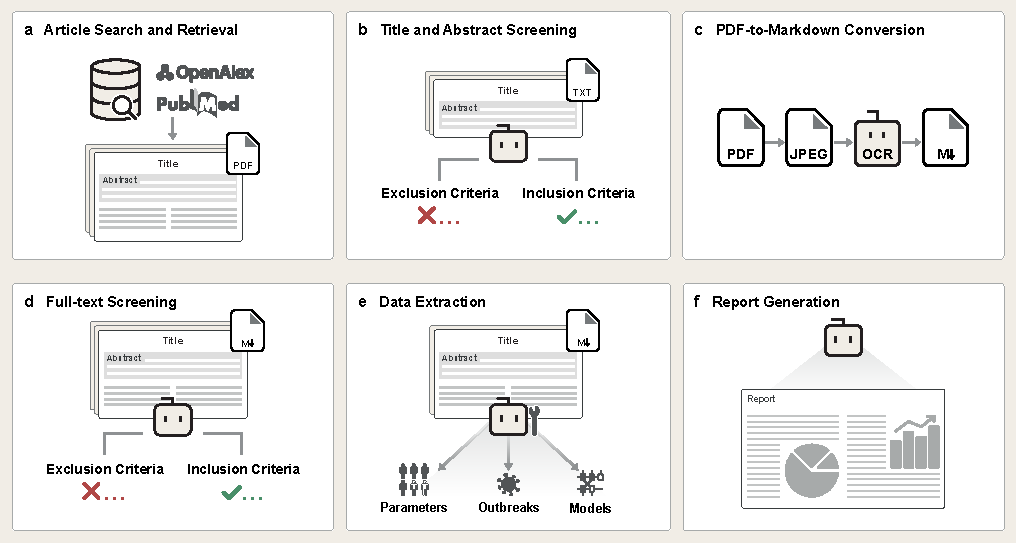
\includegraphics[width=\linewidth]{figures/flashfig_hero.pdf}
\caption{{\bf End-to-end agentic pipeline (\name) for automated systematic literature reviews}. The pipeline demonstrates a complete automation of the systematic review workflow in epidemiology, using open-source modular components. (a) \textit{Article Search and Retrieval} queries bibliographic databases with domain-specific Boolean searches and obtains PDF from open-access sources. (b) \textit{Title and Abstract Screening} applies language reasoning models to filter articles using expert-designed inclusion/exclusion criteria. (c) \textit{PDF-to-Markdown Conversion} uses an image-to-text OCR model to convert PDFs to machine-readable Markdown. (d) \textit{Full-text Screening} applies stricter filtering criteria than (b). (e) \textit{Data Extraction} employs multi-stage tool-calling with schema validation to extract structured epidemiological data (parameters, models, outbreaks). (f) \textit{Report Generation} synthesises extracted data through programmatic descriptive generation followed by iterative LRM self-refinement (writing, critique and evidence grounding). For more details see Section~\ref{sec:pipeline}.} 
\label{fig:flashfig}
\end{figure*}

% Gap:
To ground these issues in a real scientific workflow, we focus on infectious disease epidemiology as an application domain. SLRs in epidemiology often require standardised extraction of a wide range of key parameters such as the basic reproduction number, serial interval, and case-fatality ratio across diverse study designs and data representations---a task made more challenging by substantial heterogeneity in methodologies and reporting structures \citep{he2020estimation,WARD2026100882}.  We therefore select epidemiology to establish the technical feasibility of automating evidence synthesis in a specialised scientific domain. 

\vspace{1em}

% Contributions:
Our contributions are summarised as follows:
\begin{itemize}

\item We introduce \textbf{\name{}}, a fully \textit{open-source, end-to-end agentic pipeline} that uses language reasoning models (LRMs) to automate real-world systematic reviews, including article retrieval, screening, tool-based data extraction, and living systematic review generation. 

% \footnote{Code available in Supplementary Materials.}

\item We apply \name{} to epidemiology, evaluating against expert ground truth data from SLRs on WHO-designated priority pathogens. 
We demonstrate that agentic LRM systems can achieve comparable outputs to humans while processing articles $58$ times faster.

\item We validate \name{}'s extracted outputs with manual annotation by human expert epidemiologists. Annotators judge extractions to be largely accurate ($79.8\%$ average) and suggest the system would play a useful collaborative role in their review process.

\item We conduct model ablations across five frontier reasoning models (\texttt{gpt-oss-120b, GPT-5.2, Kimi-K2.5, GLM-4.7, DeepSeek-V3.2}), 
analysing the performance-to-cost trade-off across pipeline stages and identifying where model choice most impacts systematic review automation.
\end{itemize}



\section{\name{} Pipeline}\label{sec:pipeline}
We present \name{}, an end-to-end open-source AI pipeline designed to automate and streamline systematic literature reviews. It is comprised of six stages (Figure~\ref{fig:flashfig}): article retrieval, abstract and full-text screening, OCR-based PDF to markdown conversion, structured data extraction using tools and report generation. 
% The complete process runs autonomously, with human involvement during post-hoc evaluations.

%---------------------------------------------------
\subsection{Article Search and Retrieval}\label{sec:search}
\name{} queries three bibliographic databases (OpenAlex, PubMed, and Europe PMC) using domain-specific Boolean search strategies covering seven core epidemiological domains. %including transmission dynamics, disease severity, temporal parameters, and transmission heterogeneity. 
Retrieved records are first deduplicated using identifier and bibliographic metadata-based matching, then full texts are automatically retrieved from open-access sources. 
% A cascading PDF retrieval workflow follows, first enriching records with additional identifiers and then sequentially querying multiple prioritised open-access sources. 
The download pipeline incorporates caching, streaming and file validation, parallel execution and checkpointing. Full details are provided in Appendix~\ref{app:search_queries}.


%---------------------------------------------------
\subsection{Title and Abstract Screening}
Initial screening is conducted using titles and abstracts based on predefined inclusion and exclusion criteria (Appendix~\ref{app:article_screening_prompts_criteria}). We use large language reasoning models (LRMs), which enable inference-time scaling without fine-tuning on limited prior studies. Following the ScreenPrompt methodology \citep{ottoSRPromptPaper}, we structure screening with five components: study objectives, inclusion/exclusion criteria, chain-of-thought reasoning instructions, article abstract and structured output format. 

%---------------------------------------------------
\subsection{PDF-to-Markdown Conversion}\label{sec:pdf_to_markdown_conversion}
% Downloaded PDFs are converted to structured Markdown using the Mistral OCR API. 
Each downloaded PDF is rendered page-by-page into high-resolution images, then processed with an OCR model to recover text while preserving document hierarchy, equations (LaTeX), and tables (HTML). The process produces one Markdown file per article.
%---------------------------------------------------
\subsection{Full-text Screening}
Converted articles undergo full-text screening using an LRM with a prompt structure analogous to abstract screening but with stricter criteria, requiring extractable quantitative epidemiological parameters (e.g. transmission rates, incubation periods and severity outcomes) while excluding literature reviews, meta-analyses, and case studies describing fewer than 10 infected individuals. We provide the full criteria and prompts in Appendix~\ref{app:article_screening_prompts_criteri_fulltext}.

%---------------------------------------------------
\subsection{Data Extraction}\label{sec:data_extraction}
We extract structured data for three categories---epidemiological parameters, transmission models and concluded outbreaks---using a multi-stage, schema-constrained framework. Extraction is carried out by an agentic LRM with specialised tool calls to enforce field-level constraints and ensure structured outputs, mimicing human annotators extracting relevant data from articles by filling in survey forms.

For each data category, the pipeline first conducts \textit{presence flagging} to identify articles containing relevant data, followed by targeted extraction using parameter-specific, model-specific, or outbreak-specific tool calls for validated outputs. For epidemiological parameters, extraction also involves population tagging (e.g. age groups, geographic locations and clinical severity), which enables subsequent aggregation of parameter estimates into summary statistics across population contexts. Complete schemas, tool definitions and validation rules are provided in \Cref{app:data_extraction_details}.


\subsection{Report Generation}
Extracted data are converted into a structured review through a multi-stage process. Descriptive statistics are computed and visualised alongside standardised figures and evidence tables with an accompanying content manifest. An LRM generates an initial narrative synthesis, which then undergoes iterative self-refinement loops ($K=5$). Each iteration consists of a rubric-based critique assessing clarity, completeness and traceability, followed by targeted revision. During each revision, the model receives the complete evidence packet and is instructed to ensure all claims are either explicitly supported by the extracted data (figures, tables, and statistics) or clearly marked as interpretation, removing any statements that cannot be verified. The full process is detailed in \Cref{app:report_generation_methods}.


\begin{table}[t!]
\centering
\footnotesize
\caption{\textbf{Total research articles processed for creating priority pathogen SLRs.} \textbf{PERG} indicates the total article count retrieved from \texttt{epireview} (R package) after deduplication; \textbf{\name{}} indicates articles downloaded after \name{}'s Article Search and Retrieval stage; \textbf{Matched} indicates their intersection. The coloured symbols represent the progress of PERG's SLRs per priority-pathogen: published \published{}, conducting data extraction \extractionphase{}, and yet to begin screening \notstarted{}, as of March 2026.}
\setlength{\tabcolsep}{3pt}
\renewcommand{\arraystretch}{1.1}
\label{tab:article_count_summary_ours_pergs}
\begin{tabular}{lrrr}
\toprule
\textbf{Pathogen} & \textbf{PERG\textsuperscript{*}} & \textbf{\name{}} & \textbf{Matched} \\
\midrule
\published{} Marburg virus & 2,593 & 6,501 & 762 (29.4\%) \\
\published{} Ebola virus & 11,605 & 23,226 & 3,938 (33.9\%) \\
\published{} Lassa fever & 2,131 & 6,514 & 647 (30.4\%) \\
\published{} SARS-CoV-1 & 12,280 & 7,540 & 1,967 (16.0\%) \\
\published{} Zika virus & 10,510 & 3,103 & 2,128 (20.2\%) \\
\extractionphase{} MERS-CoV & 19,656 & 23,204 & 5,675 (28.9\%) \\
\extractionphase{} Nipah virus & 1,458 & 5,103 & 664 (45.5\%) \\
\notstarted{} Rift Valley fever virus & -- & 6,810 & -- \\
\notstarted{}  CCHF virus & -- & 3,478 & -- \\
\midrule
\textbf{Total}$^{\dagger}$ & 60,233 & 75,191 & 15,781 (26.2\%) \\
\bottomrule
\end{tabular}
% \vspace{0.5pt}
\par{\scriptsize
\textsuperscript{*}Articles post deduplication and empty abstract removal. \\
$^{\dagger}$Excludes Rift Valley fever virus and CCHF virus article counts.}
\end{table}



\section{Methods}

\subsection{Data}
\label{sec:methods_data}
For evaluation against ground truth, we used SLRs from the Pathogen Epidemiology Review Group (PERG) and their corresponding data made available through the \texttt{epireview} and \texttt{priority-pathogen} R packages \cite{naidooEpireviewToolsUpdate2025, nashPrioritypathogens2026}. PERG is conducting SLRs for nine ``priority pathogens'' identified by the WHO as having high epidemic or pandemic potential \cite{worldhealthorganizationPathogensPrioritizationScientific2024}. The group has published five peer-reviewed SLRs \cite{cuomo-dannenburgMarburgVirusDisease2024, doohanLassaFeverOutbreaks2024, nashEbolaVirusDisease2024, morgensternSevereAcuteRespiratory2025,mccain2026systematic} and two more (MERS and Nipah) are in the data extraction phase. For these seven pathogens, approximately $26.2\%$ of the articles considered by PERG were available under open-access licensing through the bibliographic databases we queried (\Cref{tab:article_count_summary_ours_pergs}). We evaluated each \name{} stage with all pathogen data available, meaning the first seven are evaluated for screening, and four (Ebola, Lassa, SARS, and Zika) are evaluated for data extraction. After correspondence with PERG, we chose to exclude Marburg due to inconsistencies in data format, and MERS and Nipah because PERG's extraction phase is still in progress.



\subsection{Models}
% We implemented \name{} with OpenAI's open-weight \texttt{gpt-oss-120b} model \cite{openai2025gptoss120bgptoss20bmodel}. Note that the pipeline is extensible to any model accessed via API. \texttt{gpt-oss-120b} has a context length of 131,072 tokens; articles require approximately 32,000 input tokens, and the remaining $\sim$100,000 are frequently fully used for prompt input, reasoning and tool calling. We host the model with \texttt{vllm} \cite{kwon2023efficient} using 2 NVIDIA H200 GPUs. Tool calls are schematised through the OpenAI Responses API using the Harmony Response Format.

\name{} is implemented to be compatible with both open- and closed-weight models, with tool calls and requests schematised through OpenAI's Responses and Chat Completions APIs. Unless otherwise stated, we evaluated OpenAI's open-weight \texttt{gpt-oss-120b} reasoning model for all primary results in \Cref{sec:pipeline_experimental_results} \citep{openai2025gptoss120bgptoss20bmodel}. To assess the robustness and generalisability of the pipeline across model families, we conducted ablations using OpenAI's \texttt{GPT-5.2}, Moonshot AI's \texttt{Kimi K2.5}, Z.AI's \texttt{GLM-4.7}, and DeepSeek's \texttt{DeepSeek-V3.2}. Attempts to evaluate Claude Opus 4.5 and Sonnet 4.5 resulted in streaming refusals.\footnote{We experience this refusal problem with all Claude models above version 4.0 (See \href{https://platform.claude.com/docs/en/test-and-evaluate/strengthen-guardrails/handle-streaming-refusals}{Documentation} from Anthropic). Potential causes and implications are discussed in \Cref{sec:discussion}.} All models had reasoning set to high where possible, with a maximum generation limit of 64K tokens per pass. Open-source models were hosted with \texttt{vllm} \cite{kwon2023efficient} on a NVIDIA H200 cluster node.

For the PDF-to-Markdown conversion stage, we used the \texttt{mistral-ocr-2512} API endpoint \cite{mistralaiMistralOCR32025}, a state-of-the-art OCR model well-suited to scanned documents with complex mathematical and tabular content. For reproducibility, \name{} is also configured to run with open-weight OCR models available on HuggingFace. 
% We further conduct ablations for OCR quality using DeepSeek-OCR \cite{wei2025deepseekocrcontextsopticalcompression}.
% Swapping this component yields minimal downstream differences, as we demonstrate with full ablation results in Appendix~\ref{app:xyz}.


\begin{figure}[t]
\centering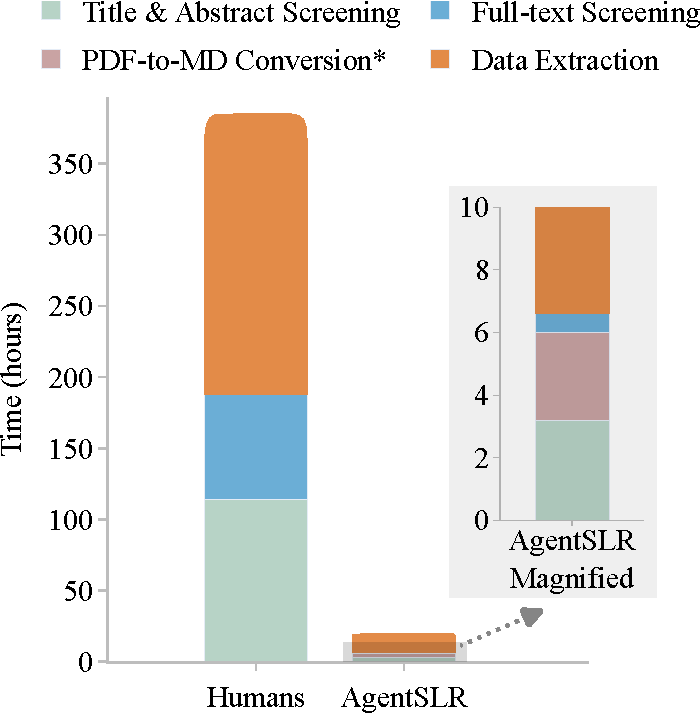
\includegraphics[width=0.375\textwidth]{figures/pipeline_stats/timeline_stats_vertical.pdf}
\caption{\textbf{Human vs. \name{} SLR completion time.} \name{} (with  \texttt{GPT-OSS-120B}) completes the end-to-end workflow in $20$ hours versus $385$ hours taken for manual-conducted reviews ({$19.3\times$} speed-up). Running continuously, this corresponds to less than 1 day ($0.83$) versus $48.1$ human workdays (assuming 8-hour days), yielding {$58\times$} calendar-time savings. Of \name{}'s run-time: data extraction accounts for $13.4$ hours ($67\%$), title and abstract screening for $3.2$ hours ($16\%$), PDF-to-MD conversion for $2.8$ hours ($14\%$), and full-text screening under $1$ hour. Times shown reflect processing of $9,132$ articles at abstract screening, $1,102$ at full-text screening and $395$ at data extraction. Report generation ($\leq$ $5$ minutes per pathogen) has been omitted. For more information, see Appendix~\ref{app:pipeline_statistics}.} \label{fig:time_comparison}
    \label{fig:time_comparison}
\end{figure}

\subsection{Metrics}

\paragraph{Pipeline runtime.} We evaluated \name{} first in terms of time efficiency relative to human annotators (\Cref{sec:full_pipeline_statistics}). We recorded the total wall-clock time to complete the first five pipeline stages and compare this time to self-reported estimates by human experts per stage. The final stage -- producing a final SLR for peer review -- does not admit a reliable time estimate, as it includes deliberations over meta-analysis outside the scope of \name{}, so we omitted this stage from our comparison.

%------------------------------
\paragraph{Individual pipeline stage evaluations.} To assess pipeline quality, we validated against expert annotations on four priority pathogens: Ebola, Lassa, SARS and Zika. 
We designed stage-level evaluations for each of abstract screening, full-text screening and data extraction. To isolate stage-level performance from compounding errors, each evaluation used ground-truth inputs for all previous stages.

Each of the two article screening stages is framed as a binary classification task, so we considered classification metrics (precision, recall, and $F_1$) against ground-truth screening decisions. Because the screening task is highly imbalanced, with far more excluded than included articles, we report these metrics and prioritise recall: false inclusions are easier to rectify at later pipeline stages, whereas missing articles cannot be corrected. For data extraction, quantifying agreement with ground-truth annotations is less straightforward. Each article may contain arbitrarily many extractions, and individual extractions may differ across many metadata fields. For a holistic account of \name's performance, we designed three evaluation measures. \textit{Flagging} assesses how reliably our pipeline identifies relevant parameter classes, models and outbreaks within an article. \textit{Count} measures agreement in the number of extracted items per article. \textit{Extraction} measures field-level accuracy by computing bipartite matches between our extractions and ground-truth extractions that maximise overall similarity. \Cref{app:additional_evaluation_details} provides formal definitions of the evaluation metrics and outlines pre-processing steps.
%------------------------------


\begin{figure*}[t!]
    \centering
    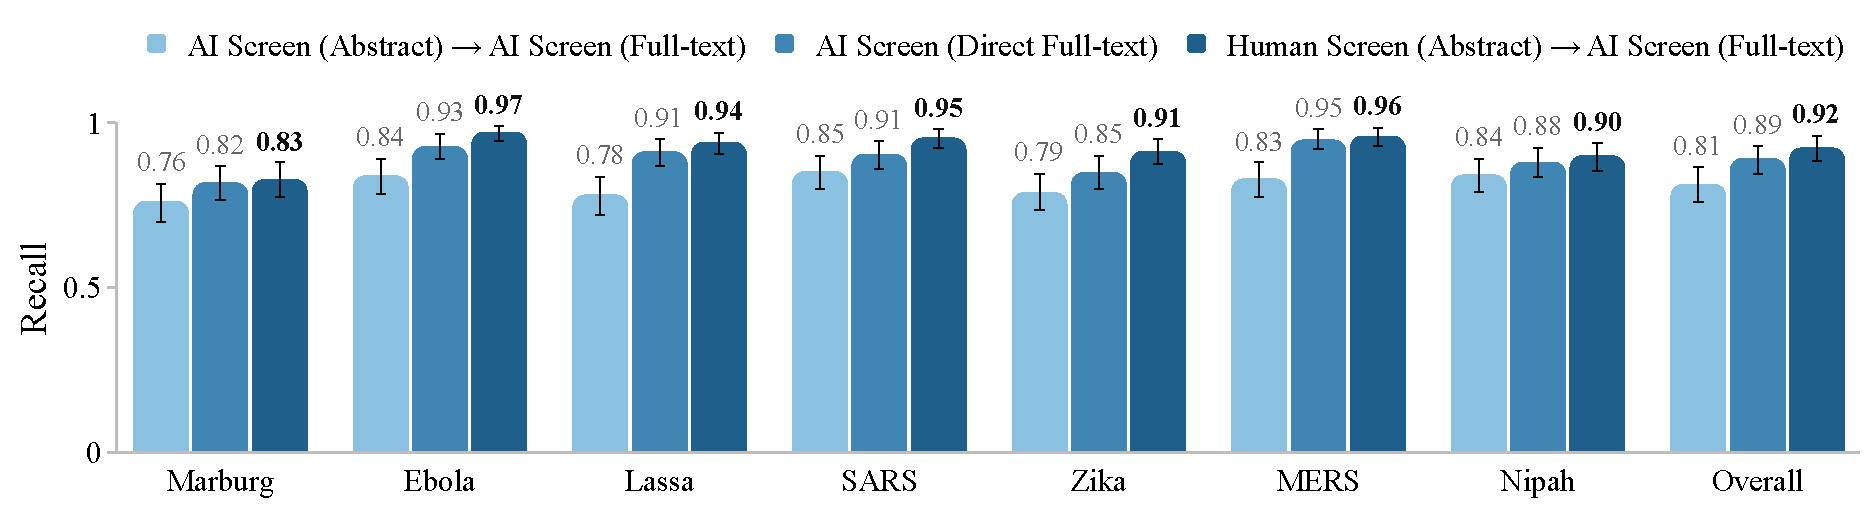
\includegraphics[width=1\linewidth]{figures/results/article_screening_recall.pdf}
    \caption{\textbf{Recall of article screening strategies across pathogens.} Two ablation screening strategies (human-conditioned, direct full-text) with \name{} (\texttt{GPT-OSS-120B}) offer better recall (or `fetch rate') than performing traditional AI-based two stage screening, with bootstrapped confidence intervals (95\% C.I.; 10{,}000 resamples) between the two ablations overlapping across most pathogens. Full article screening metrics along with individual title \& abstract stage screening results are reported in \Cref{app:extended_results_article_screening}.}
    \label{fig:fulltext_recall_barchart}
\end{figure*}

\paragraph{Human expert validation.}\label{sec:human_expert_validation_methods} Ground-truth screening decisions and annotations provide clear standards for recall---they allow us to check whether \name{} retrieves all relevant data. However, with respect to precision, it is ambiguous whether additional extractions represent genuine false positives or were instead missed by human annotators due to cognitive bandwidth constraints.

To supplement our individual stage evaluations, we conducted an additional validation with six expert epidemiologists. Each expert was assigned a random subset of extracted data for parameters, models or outbreaks, along with the corresponding markdown articles, and asked to grade extraction correctness using a survey. Survey questions included a yes/no question on the overall relevance of the extraction, yes/no questions for individual field correctness, and a holistic rating of \name{}'s capability for the task. For field-level correctness, we grouped fields by category (e.g. temporal features or population context) and reported normalised accuracy to assign equal importance to each group. Overall system capability was measured through ratings ranging between $1$ and $7$, where $1$ means total incompetence at the task, $4$ is the threshold for a useful tool under human supervision, and $7$ means completely competent and autonomous. System capability was rated for each extraction, providing a distribution of scores. \Cref{app:human_expert_validation} describes the survey design and implementation.



%%%%%%%%%%%%%%%%%%%%%%%%%%%%
% Results
%%%%%%%%%%%%%%%%%%%%%%%%%%%%%
\section{Results}\label{sec:pipeline_experimental_results}

\subsection{Full Pipeline Statistics}\label{sec:full_pipeline_statistics}
We demonstrate the base functionality of \name{} by running our pipeline for all nine priority pathogens using \texttt{gpt-oss-120b}. \name{} completes each report with an average wall clock time of $20$ hours, processing $9,132$ articles at title/abstract screening, $1,102$ at full-text screening and $395$ at data extraction.\footnote{We consider articles processed at each stage based on average across pathogens. See \cref{app:perg_pipeline} for more details.} \Cref{app:report_writeup} explains the report generation process in detail. \Cref{fig:time_comparison} shows the time comparison to human expert estimates, where \name{}'s runtime ($\le$ 1 day) represents a $19.3$-times efficiency gain over the corresponding human processes ($385$ hours).  Since \name{} runs continually, our runtime equates to a 
$58$-times reduction in calendar days (assuming $8$-hour workdays for 
humans). For full-text screening in particular, \name{} is $118$ times faster than humans, reducing a $4$-minute average down to below $2$ seconds per article.  The average cost of running \name{} per SLR varies by model and deployment: for example, self-hosting \texttt{gpt-oss-120b} on two Nvidia H200 GPUs costs approximately USD\$137,\footnote{This cost estimate includes OCR PDF-to-markdown conversion using \texttt{mistral-ocr-2512}.} while using the OpenRouter API reduces the cost to USD\$50 with higher latency as a trade-off. \Cref{app:pipeline_statistics_costs} provides detailed comparisons across models and services.

% Assuming USD\$2.50 per H200 per hour (2 GPUs) plus USD\$36.60 for OCR ($1,102$ articles $\times$ $16.7$ pages at USD\$2 per 1,000 pages via Mistral OCR 3), we estimate a total cost of USD\$137.00 per report for \texttt{gpt-oss-120b}. Costs for ablation models via both H200 and OpenRouter API are provided in Appendix~\ref{app:pipeline_statistics}.}

%, includes \myred{$X$}, and extracts \myred{$X$} data points. This process produces nine novel reports on the evidence base for each pathogen, which we provide in \myred{Appendix X}. \Cref{app:pipeline_statistics} presents further runtime statistics broken down by pathogen and pipeline stage.

%%%%%%%%%%%%%%%%%%%%%%%%%%%%%%%%%%%%%%%%%%%%%%%
% Results — Evaluation Against Ground-truth
%%%%%%%%%%%%%%%%%%%%%%%%%%%%%%%%%%%%%%%%%%%

\subsection{Evaluation Against Ground-truth}\label{sec:PERG_data_evaluation}



\begin{figure*}[t!]
    \centering
    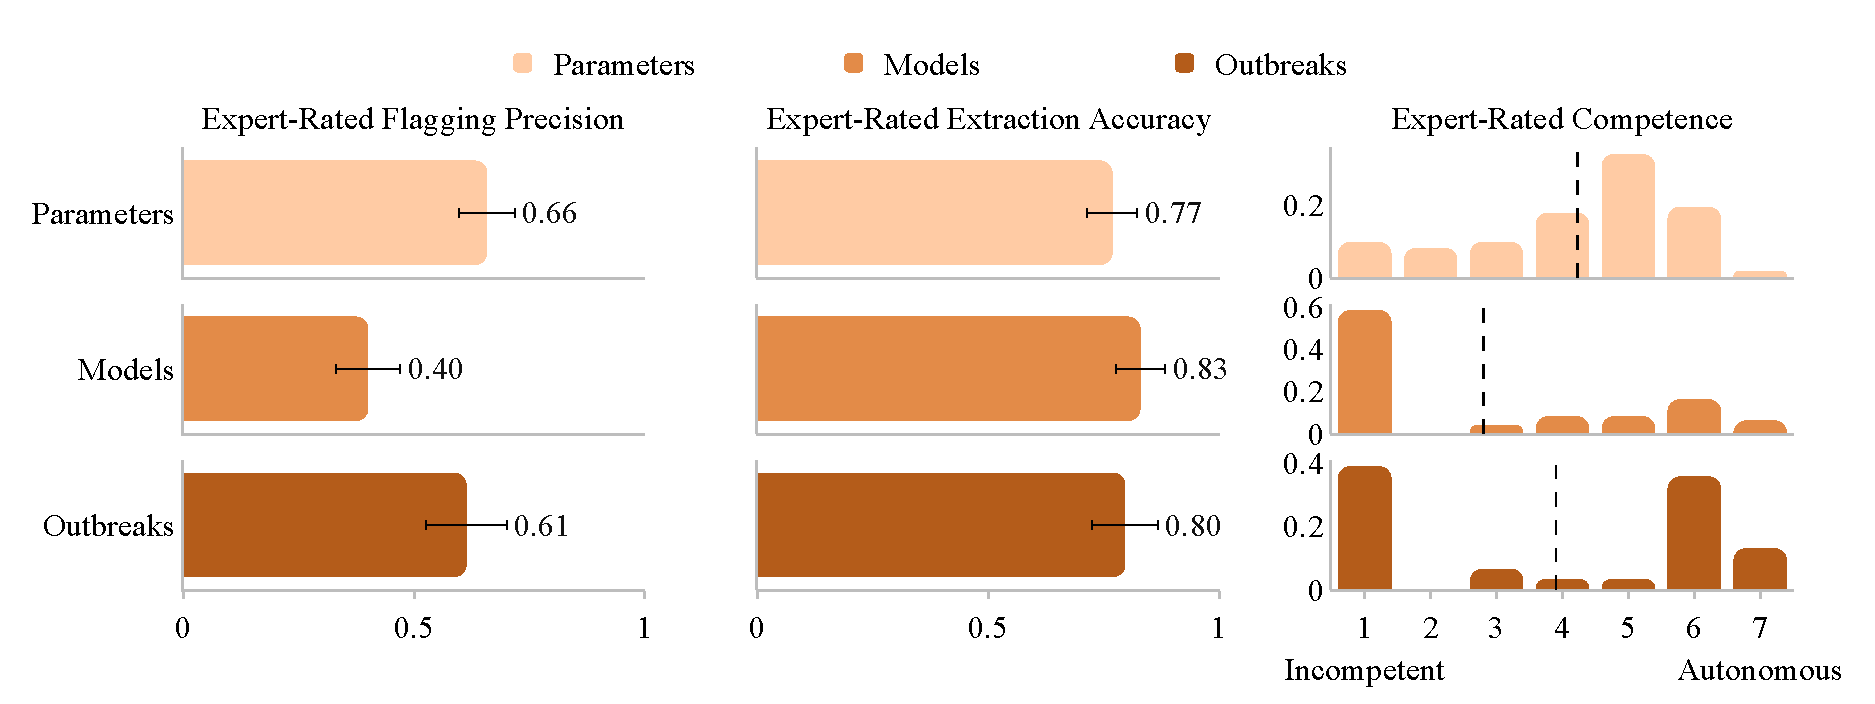
\includegraphics[width=\linewidth]{figures/results/expert_survey.pdf}
    \caption{\textbf{Human expert evaluation of data extraction quality across stages.} We report expert-rated flagging precision, field-level extraction accuracy, and perceived \name{} (\texttt{gpt-oss-120b}) competence for parameter, model, and outbreak extractions, aggregated across six epidemiologists. Error bars denote standard errors, and dashed lines indicate mean competence ratings ($4.2$ for parameters, $2.8$ for models, and $3.9$ for outbreaks).}
    \label{fig:expert_validation_results}
\end{figure*}

%%




\begin{figure*}[t]
    \centering
    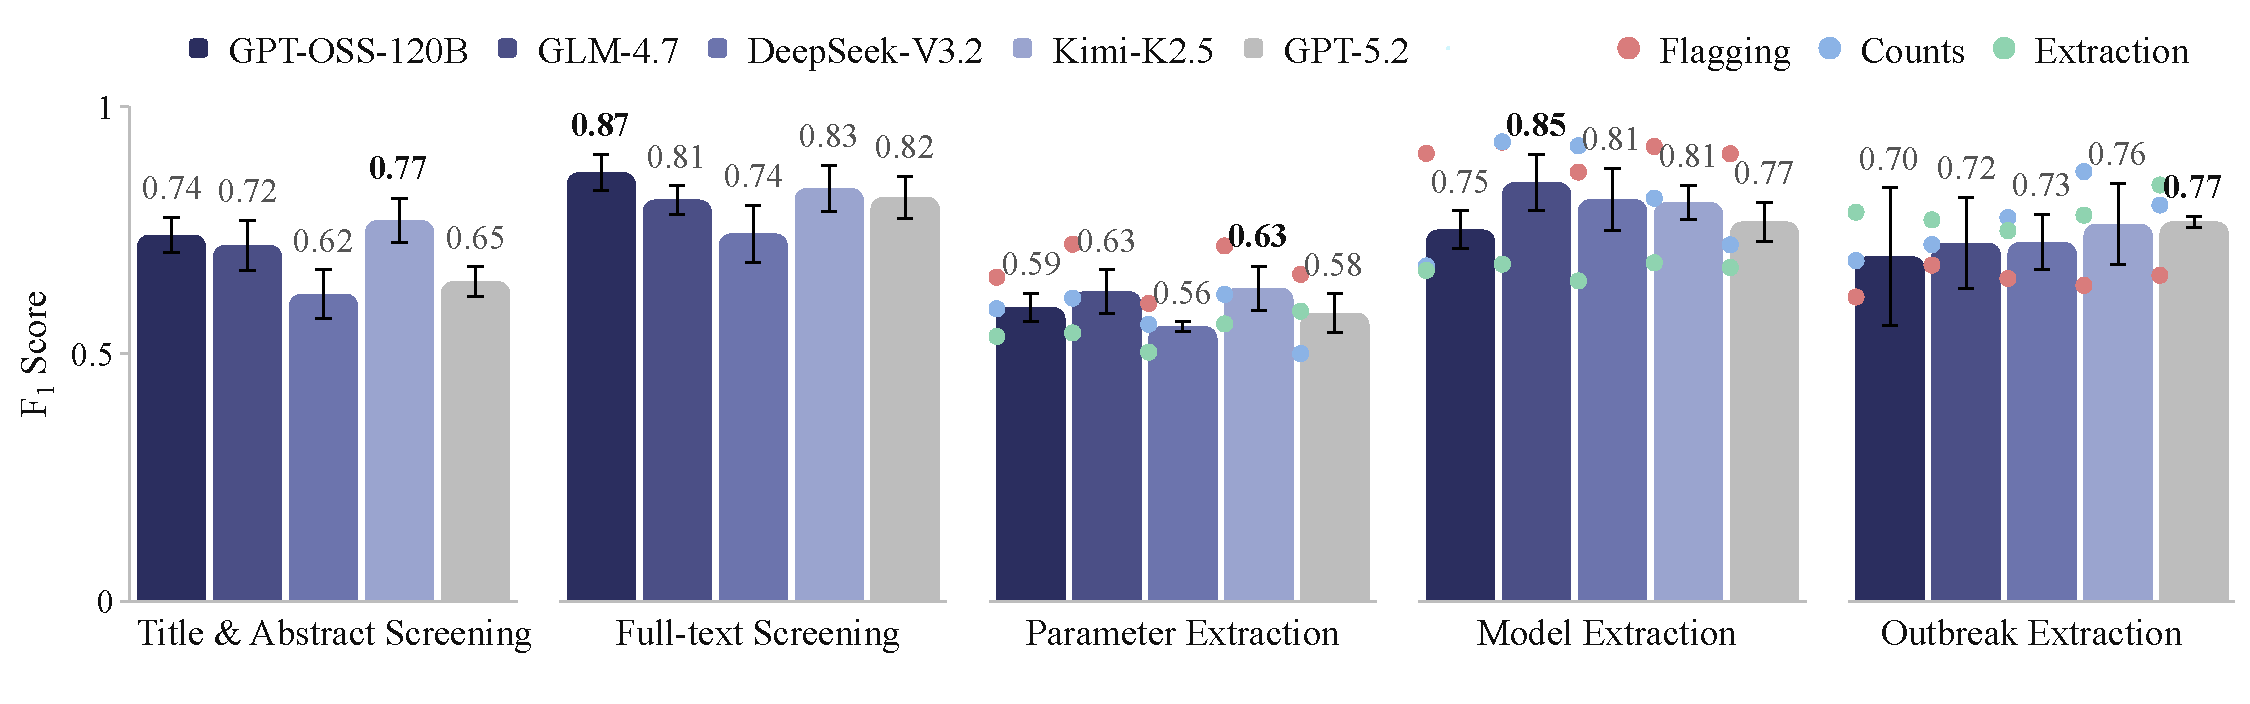
\includegraphics[width=\textwidth]{figures/ablation/model_ablations.pdf}
    \caption{\textbf{Model ablation results with \name{} across all pipeline stages.} Macro F1 is reported for five client models, evaluated separately for each pathogen. Averages are computed over the pathogens evaluated at each stage, following ground-truth availability described in Section~\ref{sec:methods_data}. Error bars indicate one standard deviation across pathogens. For the three data extraction panels, coloured dots show the macro F1 of the Flagging \deflagging{}, Counts \decounts{}, and Extraction \deextraction{} sub-tasks, plotted to the left of each bar. No single model dominates across all stages: \texttt{Kimi-K2.5} and \texttt{gpt-oss-120b} lead screening, while extraction leaders vary by data type. Full pathogen-wise metrics are provided in Appendix~\ref{app:model_ablations}.}
    \label{fig:model_ablation}
\end{figure*}


%%%%%%%%%%%%%%%%%%%%%%%%%%%%%%%%%%%%%%%%%%%%%%%%%%%%
% Evaluation Against Ground-truth — Article Screening
%%%%%%%%%%%%%%%%%%%%%%%%%%%%%%%%%%%%%%%%%%%%%%%%%%%%
\paragraph{Article screening.}
\Cref{fig:fulltext_recall_barchart} compares three article screening strategies tested across the seven evaluated pathogens. Under the default two-stage screening pipeline, \name{} achieves a recall of $0.81$ against ground-truth screening decisions. To contextualise this performance, we consider two ablations. First, we condition full-text screening on ground-truth (human) abstract screening decisions, which improves recall to $0.92$. Second, we omit abstract screening and process all full-texts directly, which improves recall to $0.89$. Both trends are consistent across pathogens (\Cref{fig:fulltext_recall_barchart}). Direct full-text screening thus improves recall over the two-stage pipeline without human involvement, though at a $2.3\times$ increase in screening runtime ($9.55$ vs $4.16$ hours) and a corresponding rise in OCR costs (USD\$36.6 vs USD\$303.2).

\paragraph{Data extraction.}
\Cref{tab:data_extraction_metrics} presents our evaluation results for parameter, model and outbreak extraction. We report average classification measures (precision, recall and $F_1$) for each of our Flagging, Count and Extraction metrics. Across all data types, flagging achieves the highest average $F_1$ ($0.75$), with performance declining progressively through counting ($0.65$) and extraction ($0.63$), reflecting the compounding difficulty of each successive pipeline stage.
See \Cref{app:data_extraction_extended} for complete disaggregated results across all data subtypes, pathogens and individual fields.

%\paragraph{Parameter Extraction} 
\name{} displays high recall ($0.92$) but moderate precision ($0.51$) for parameter class flagging. For parameter extraction counts, this trend reverses, suggesting that the agent identifies many parameter classes as potentially relevant, yet exercises more discretion when producing structured extractions. At the field level, performance is moderate across all pathogens. \name{} achieves near-perfect accuracy for method extraction and for specific uncertainty fields (notably single-type uncertainty), while value fields and population context prove considerably more challenging (See \cref{tab:parameters_detailed_metrics}). 

%\paragraph{Model Extraction} 
\name's model extraction achieves strong flagging performance, with high recall ($0.91$) and precision ($0.90$). This high recall carries through to model counts ($0.99$), indicating that nearly all models from the ground truth data are recovered, albeit with lower precision for counting ($0.52$). At the field level, model extraction attains a precision of $0.63$ and recall of $0.74$: core structural characteristics (model type, stochastic vs.\ deterministic and code availability) are extracted reliably, while complex multi-value fields such as assumptions, interventions and transmission routes remain more challenging (See \cref{tab:models_detailed_metrics} for the complete results).



\begin{table}[b!]
\centering
\caption{\textbf{Evaluation metrics for data extraction stage (averaged across pathogens with $\pm$ deviation).} Results for \name{} (\texttt{gpt-oss-120b}) are reported separately for \textit{Flagging}, \textit{Count}, and \textit{Extraction}, measuring presence identification, quantity accuracy, and value accuracy, respectively. Flagging achieves the strongest performance ($F_1 = 0.75$), followed by counting and extraction. For disaggregated metrics, see \Cref{app:data_extraction_extended}.}
\label{tab:data_extraction_metrics}
\footnotesize
\setlength{\tabcolsep}{3.5pt}
\renewcommand{\arraystretch}{0.97}
\begin{tabular}{lccc}
\toprule
\textbf{Data Type} & \textbf{Precision} & \textbf{Recall} & \textbf{$F_1$ Score} \\
\midrule
\multicolumn{4}{l}{\textbf{Parameters}} \\
\quad \deflagging{} Flagging   & 0.51 ($\pm$ 0.07) & 0.92 ($\pm$ 0.06) & 0.66 ($\pm$ 0.06) \\
\quad \decounts{} Count      & 0.83 ($\pm$ 0.10) & 0.47 ($\pm$ 0.09) & 0.59 ($\pm$ 0.07) \\
\quad \deextraction{} Extraction & 0.52 ($\pm$ 0.03) & 0.57 ($\pm$ 0.04) & 0.54 ($\pm$ 0.02) \\

\midrule

\multicolumn{4}{l}{\textbf{Models}} \\
\quad \deflagging{} Flagging   & 0.90 ($\pm$ 0.04) & 0.91 ($\pm$ 0.05) & 0.91 ($\pm$ 0.04) \\
\quad \decounts{} Count      & 0.52 ($\pm$ 0.05) & 0.99 ($\pm$ 0.01) & 0.68 ($\pm$ 0.04) \\
\quad \deextraction{} Extraction & 0.63 ($\pm$ 0.04) & 0.74 ($\pm$ 0.02) & 0.67 ($\pm$ 0.03) \\

\midrule

\multicolumn{4}{l}{\textbf{Outbreaks}} \\
\quad \deflagging{} Flagging   & 0.63 ($\pm$ 0.06) & 0.76 ($\pm$ 0.05) & 0.61 ($\pm$ 0.09) \\
\quad \decounts{} Count      & 0.66 ($\pm$ 0.17) & 0.72 ($\pm$ 0.28) & 0.69 ($\pm$ 0.22) \\
\quad \deextraction{} Extraction & 0.85 ($\pm$ 0.00) & 0.76 ($\pm$ 0.02) & 0.79 ($\pm$ 0.01) \\

\midrule

\multicolumn{4}{l}{\textbf{Average (across data types)}} \\
\quad \deflagging{} Flagging   & 0.70 ($\pm$ 0.05) & 0.88 ($\pm$ 0.04) & 0.75 ($\pm$ 0.06) \\
\quad \decounts{} Count      & 0.67 ($\pm$ 0.09) & 0.73 ($\pm$ 0.06) & 0.65 ($\pm$ 0.06) \\
\quad \deextraction{} Extraction & 0.62 ($\pm$ 0.07) & 0.67 ($\pm$ 0.03) & 0.63 ($\pm$ 0.05) \\

\bottomrule
\end{tabular}
\end{table}


%\paragraph{Outbreak Extraction} 
We evaluate outbreak extraction only for Lassa and Zika due to a lack of human annotation for Ebola and SARS. Article flagging shows moderate performance across both pathogens (precision $0.63$, recall $0.76$), and outbreak counting shows high variance ($\pm 0.28$ for recall) driven by pathogen-level differences. Despite this, field-level extraction is robust: outbreak extraction achieves the highest precision ($0.85$) amongst all data types, with particular strength in temporal features and case burden (See \cref{tab:outbreak_detailed_metrics}).

%%%%%%%%%$%%%%%$%%%%%%%%%$%%%%%%%%%$%%%%%%%%%$%%%%%%%%%$
% OLD Formatting — Data Extraction Table (ICML Submission
%%%%%%%%%%%%%%%$%%%%%%%%%$%%%%%%%%%$%%%%%%%%%$%%%%%%%%%$


%%%%%%%%%%%%% Table with new (corrected) Param extraction values %%%%%%%%%%%%
% \begin{table*}[t]
%     \centering
%     \caption{\textbf{Evaluation metrics for data extraction stage of \name{} pipeline (with \texttt{gpt-oss-120b}).} \textit{Flagging} validates how well the model identifies the presence of individual data components (epidemiological parameters, transmission models and concluded outbreaks) in each article. \textit{Count} validates the accuracy of extracted quantities, ensuring whether the model correctly identifies the number of data components per article. \textit{Extraction} validates the accuracy of specific values extracted from articles, grouped along data component lines.}
%     \label{tab:data_extraction_metrics}
%     \begin{footnotesize}
%     \begin{tabular}{ll|ccc|ccc|ccc}
%         \toprule
%         \bf \multirow{2}{*}{Data type} & \bf \multirow{2}{*}{Pathogen} & \multicolumn{3}{c|}{\textbf{Flagging}} & \multicolumn{3}{c|}{\textbf{Count}} & \multicolumn{3}{c}{\textbf{Extraction}} \\
%          & & $P$ & $R$ & $F_1$ & $P$ & $R$ & $F_1$ & $P$ & $R$ & $F_1$ \\
%          \midrule
%          \multirow{5}{*}{Parameters} & Lassa & 0.557 & 0.982 & 0.711 & 1.000 & 0.346 & 0.514 & 0.578 & 0.535 & 0.551 \\
%         & Ebola & 0.596 & 0.917 & 0.722 & 0.794 & 0.470 & 0.590 & 0.485 & 0.539 & 0.501 \\
%         & SARS & 0.500 & 0.815 & 0.620 & 0.804 & 0.610 & 0.694 & 0.514 & 0.633 & 0.558 \\
%         & Zika & 0.403 & 0.957 & 0.567 & 0.720 & 0.468 & 0.567 & 0.515 & 0.574 & 0.531 \\
%          \cmidrule{2-11}
%          & Average & 0.514 & 0.918 & \multicolumn{1}{c|}{0.655} &  0.829 & 0.473 & \multicolumn{1}{c|}{0.591} & 0.523 & 0.570 & 0.535 \\
%          \midrule
%          \multirow{5}{*}{Models} & Lassa & 0.909 & 1.000 & 0.952 & 0.600 & 1.000 & 0.750 & 0.687 & 0.699 & 0.690 \\
%          & Ebola & 0.876 & 0.952 & 0.912 & 0.500 & 1.000 & 0.667 & 0.606 & 0.680 & 0.636 \\
%          & SARS & 0.841 & 0.841 & 0.841 & 0.486 & 0.971 & 0.648 & 0.610 & 0.683 & 0.638 \\
%          & Zika & 0.785 & 0.911 & 0.843 & 0.483 & 0.977 & 0.646 & 0.683 & 0.753 & 0.706 \\
%          \cmidrule{2-11}
%          & Average & 0.853 & 0.926 & 0.887 & 0.517 & 0.987 & 0.678 & 0.647 & 0.704 & 0.668 \\
%          \midrule
%          \multirow{3}{*}{Outbreaks} & Lassa & 0.690 & 0.816 & 0.705 & 0.833 & 1.000 & 0.909 & 0.864 & 0.740 & 0.778 \\
%          & Zika & 0.576 & 0.713 & 0.525 & 0.489 & 0.449 & 0.468 & 0.870 & 0.780 & 0.812 \\
%          \cmidrule{2-11}
%          & Average & 0.633 & 0.765 & 0.615 & 0.661 & 0.724 & 0.689 & 0.867 & 0.760 & 0.795 \\
%           \midrule
%           \bf Average & & 0.644 & 0.905 & 0.718 & 0.649 & 0.757 & 0.664 & 0.720 & 0.723 & 0.710 \\
%           \bottomrule
%     \end{tabular}
%     \end{footnotesize}
% \end{table*}


%%%%%%%%%%%%% Table with original (official ICML submission) Param extraction values %%%%%%%%%%%%

% \newcolumntype{C}{>{\centering\arraybackslash}X}




% \begin{table*}[t]
% \footnotesize
%     \centering
%     \caption{\textbf{Evaluation metrics for data extraction stage of \name{} pipeline.} \textit{Flagging} validates how well the model identifies the presence of individual data components (epidemiological parameters, transmission models and concluded outbreaks) in each article. \textit{Count} validates the accuracy of extracted quantities, ensuring whether the model correctly identifies the number of data components per article. \textit{Extraction} validates the accuracy of specific values extracted from articles, grouped along data component lines.\SP{Add Table is specific to gpt-oss-120b}}
%     \label{tab:data_extraction_metrics}
%     %\scriptsize
%     \begin{tabularx}{0.95\textwidth}{ll|CCC|CCC|CCC}
%         \toprule
%         \bf \multirow{2}{*}{Data type} & \bf \multirow{2}{*}{Pathogen} & \multicolumn{3}{c|}{\textbf{Flagging}} & \multicolumn{3}{c|}{\textbf{Count}} & \multicolumn{3}{c}{\textbf{Extraction}} \\
%          & & $P$ & $R$ & $F_1$ & $P$ & $R$ & $F_1$ & $P$ & $R$ & $F_1$ \\
%          \midrule
%          \multirow{5}{*}{Parameters} & Lassa & 0.438 & 0.955 & 0.600 & 0.800 & 0.545 & 0.649 & 0.594 & 0.655 & 0.615 \\
%                                      & Ebola & 0.510 & 0.958 & 0.665 & 0.798 & 0.538 & 0.643 & 0.581 & 0.604 & 0.583 \\
%                                      & SARS  & 0.463 & 0.954 & 0.623 & 0.909 & 0.667 & 0.769 & 0.548 & 0.655 & 0.573 \\
%                                      & Zika  & 0.352 & 0.949 & 0.514 & 0.596 & 0.418 & 0.491 & 0.519 & 0.581 & 0.541 \\
%          \cmidrule{2-11}
%          & Average & 0.441 & 0.954 & \multicolumn{1}{c|}{0.601} & 0.776 & 0.542 & \multicolumn{1}{c|}{0.638} & 0.561 & 0.624 & 0.578 \\
%          \midrule
%          \multirow{5}{*}{Models} & Lassa & 0.909 & 1.000 & 0.952 & 0.600 & 1.000 & 0.750 & 0.687 & 0.699 & 0.690 \\
%          & Ebola & 0.876 & 0.952 & 0.912 & 0.500 & 1.000 & 0.667 & 0.606 & 0.680 & 0.636 \\
%          & SARS & 0.841 & 0.841 & 0.841 & 0.486 & 0.971 & 0.648 & 0.610 & 0.683 & 0.638 \\
%          & Zika & 0.785 & 0.911 & 0.843 & 0.483 & 0.977 & 0.646 & 0.683 & 0.753 & 0.706 \\
%          \cmidrule{2-11}
%          & Average & 0.853 & 0.926 & 0.887 & 0.517 & 0.987 & 0.678 & 0.647 & 0.704 & 0.668 \\
%          \midrule
%          \multirow{3}{*}{Outbreaks} & Lassa & 0.690 & 0.816 & 0.705 & 0.833 & 1.000 & 0.909 & 0.864 & 0.740 & 0.778 \\
%          & Zika & 0.576 & 0.713 & 0.525 & 0.489 & 0.449 & 0.468 & 0.870 & 0.780 & 0.812 \\
%          \cmidrule{2-11}
%          & Average & 0.633 & 0.765 & 0.615 & 0.661 & 0.724 & 0.689 & 0.867 & 0.760 & 0.795 \\
%           \midrule
%           \bf Average & & 0.644 & 0.905 & 0.718 & 0.649 & 0.757 & 0.664 & 0.720 & 0.723 & 0.710 \\
%           \bottomrule
%     \end{tabularx}
% \end{table*}
\subsection{Human Expert Validation}\label{sec:human_expert_validation}

\paragraph{Quantitative survey statistics.}
\Cref{fig:expert_validation_results}
displays results from the human expert validations on \name{} (\texttt{gpt-oss-120b}) described in \Cref{sec:human_expert_validation_methods}.
Extraction Accuracy reports the average rate of field-level correctness conditional on the extraction being correctly flagged as relevant. In contrast, Expert-Rated Competence is assessed for every case, including incorrect flaggings.
\textit{Flagging Precision} reports the proportion of \name{} extractions judged relevant by experts and is higher for parameters ($0.66$) and outbreaks ($0.61$) than for models ($0.40$). \textit{Extraction Accuracy} reports the average rate of field-level correctness. All extraction types achieve expert-rated correctness comparable to or exceeding the precision of our automated Extraction evaluation in \Cref{sec:PERG_data_evaluation} ($0.77$ for parameters; $0.83$ for models; $0.80$ for outbreaks). Finally, average \textit{Expert-Rated Competence} is $4.2$ for parameters, $2.8$ for models, and $3.9$ for outbreaks.

\paragraph{Qualitative impressions.}
Based on survey feedback from six expert epidemiologists, \name{} was consistently reported to improve efficiency compared to fully manual extractions. Although false positives occur, these are typically easy to identify and remove, resulting in a net reduction in effort. Extraction difficulty varies across papers due to differences in complexity and reporting style, and in rare cases the system may increase effort in situations that are similarly challenging for human reviewers. Once an extraction is produced, individual fields are straightforward to validate, whereas multi-select fields pose more difficulty. Common errors arise from insufficient contextual information, limited use of document structure and cross-extraction constraints, and failures to infer fields apparent to human annotators when information is implicit. Additionally, the system struggles to understand provenance, occasionally mixing up newly reported findings with information cited from prior work.

% Expanded version of the above
%The system improves extraction efficiency compared to fully manual extractions. While it produces false positives, these are typically easy to identify and remove, preserving an overall net reduction in effort. Extraction difficulty varies by paper due to differences in complexity and reporting style, and in rare cases the system may increase effort in situations that are similarly non-trivial for human reviewers. An additional challenge arises from overlapping terminology within the field, including shared terms and units, which the system struggles to differentiate; extractions often appear to be driven by keyword presence rather than holistic reasoning.

%Once an extraction is produced, individual fields are straightforward to validate, whereas multi-select fields are more challenging. Errors arise from multiple sources. Insufficient global parameter context can cause fields to be populated in isolation without fully accounting for interdependencies, resulting in logically implausible extractions. Limited incorporation of document structure and weak enforcement of distinctness across extractions can lead to information being conflated across records. In addition, the system may fail to infer fields that are apparent to human annotators when such information is not stated explicitly in the text. Separately, weak restriction of provenance can cause newly reported findings to be mixed with information cited from prior work.



\section{Model Ablations}\label{sec:model_ablations}
To contextualise the performance of \texttt{gpt-oss-120b}, we ran \name{} with four additional frontier LRMs, conducting ground-truth evaluations for each stage. We find variation in performance across stages with no clear best model (\cref{fig:model_ablation}). \texttt{Kimi-K2.5} and \texttt{gpt-oss-120b} perform best at the article screening stages, with the former excelling in title \& abstract screening ($F_1 = 0.77$) and the latter in full-text screening($F_1 = 0.63$). All models struggle with parameter extraction, with the highest performance again achieved by \texttt{Kimi-K2.5} ($F_1 = 0.87$). \texttt{GLM-4.7} performs well specifically for extracting models, while \texttt{GPT-5.2} stands out when extracting outbreaks. \texttt{DeepSeek-V3.2} exhibits the most variable performance across stages. It is the worst-performing model by some margin during article screening, but becomes competitive during the extraction phase where it is enabled with function calling, most evidently in model and outbreak extraction.

The smallest model by size, \texttt{gpt-oss-120b}, performs within $4.5$ percentage points of the best model across all stages. The next smallest model, \texttt{GLM-4.7}, is nearly $3$ times larger at $358$ billion parameters. % (spread: $-3$, $+3$, $-4$, $-10$, $-7$).
Excluding outbreak extraction, where results are aggregated only across Zika and Lassa, \texttt{gpt-oss-120b} also exhibits one of the lowest variances across pathogens. The weaker outbreak extraction performance is driven by Zika ($F_1 = 0.60$), where \texttt{gpt-oss-120b} struggles consistently across stages. We suspect this performance to be due to greater domain overlap and multi-pathogen co-occurrence, as Lassa outbreak extraction remains strong ($F_1 = 0.80$). 

\begin{figure}[t!]
    \centering
    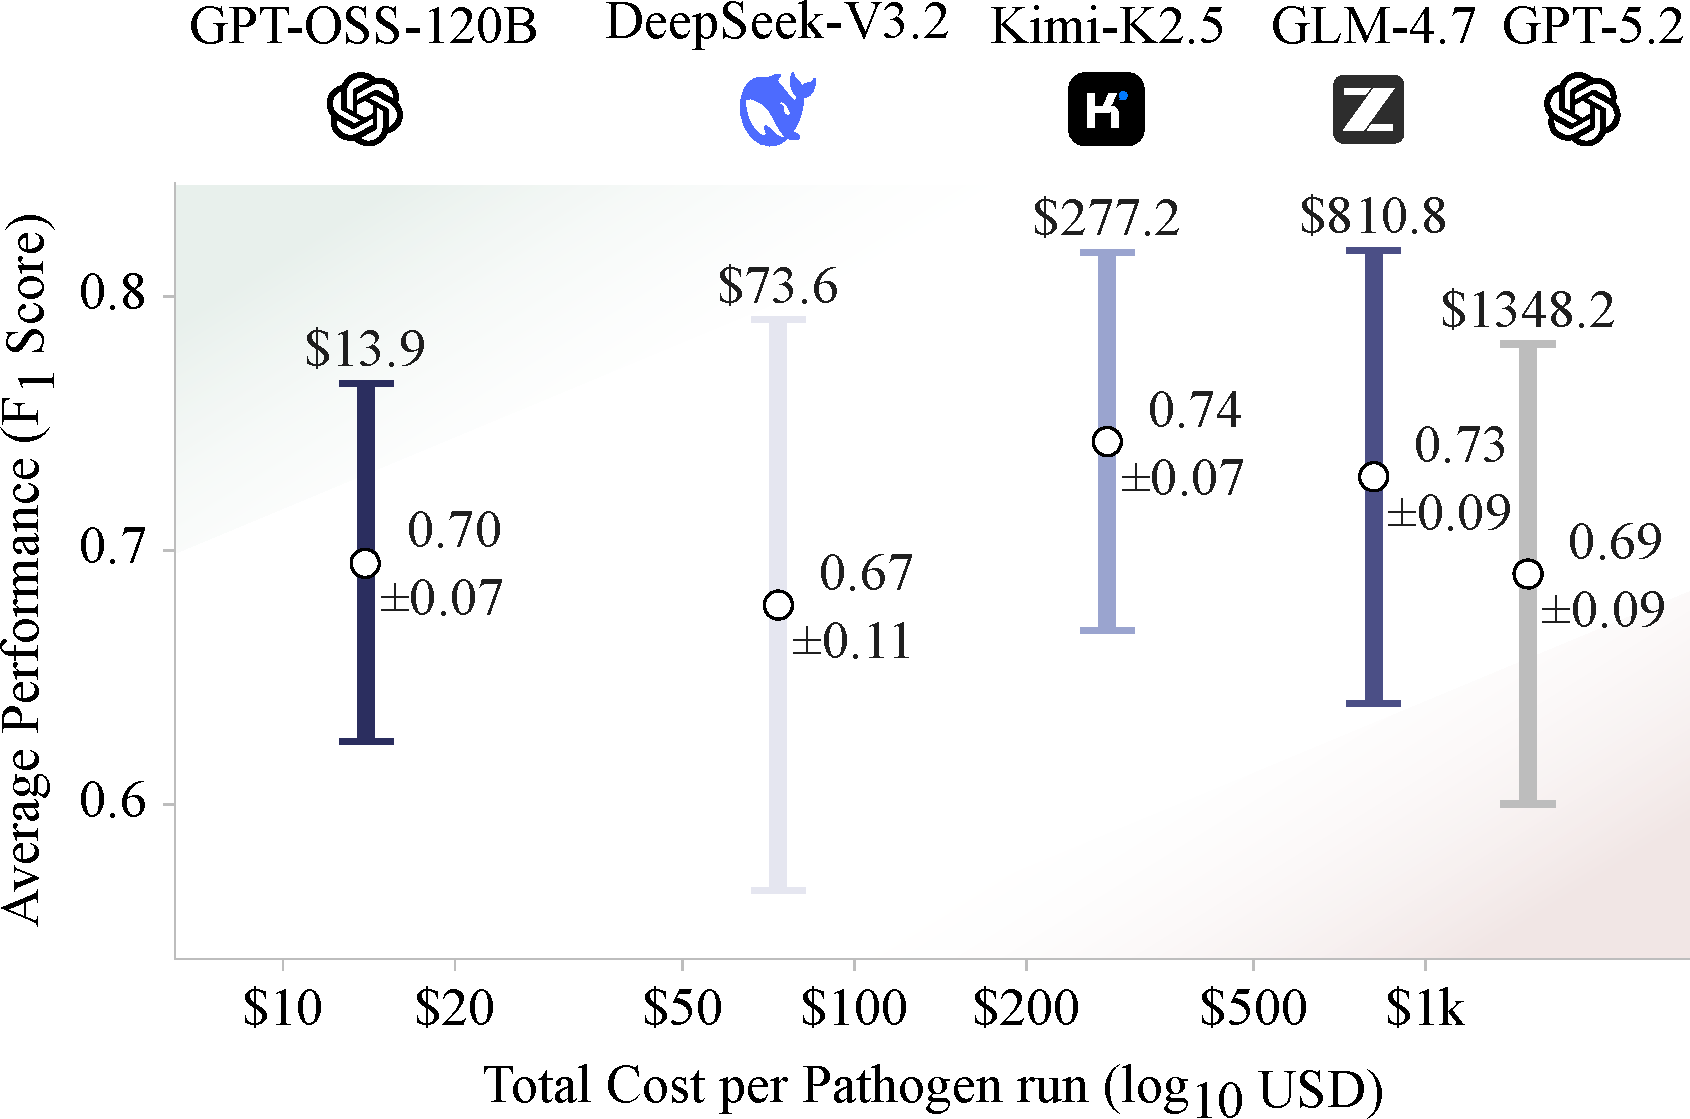
\includegraphics[width=\linewidth]{figures/ablation/cost_vs_accuracy_edited.pdf}
    \caption{\textbf{Comparing total cost against average performance for an \name{} pathogen run.} Each point shows a model's average macro $F_1$ across all \name{} pipeline stages plotted against its estimated total cost per pathogen run (USD, $\log_{10}$ scale), with vertical bars indicating one standard deviation in $F_1$ across stages. Costs are estimated from mean per-article token usage across a funnel of $9{,}132$ articles at abstract screening down to $395$ at data extraction (see \cref{fig:time_comparison} counts), multiplied by OpenRouter and OpenAI API pricing; full details in \cref{app:pipeline_statistics_costs}. We find that higher cost does not consistently correspond to higher performance.}
    \label{fig:cost_vs_performance}
\end{figure}


Consistent with \cref{tab:data_extraction_metrics}, models find the successive data extraction sub-tasks progressively harder: Flagging typically outperforms both Counts and Extraction. Outbreaks remain the exception to this trend, consistently across models, with precision notably lower for Flagging. Outbreak events are typically reported once but repeated across many papers as disease background. Across all extraction stages, the gap between the best and worst performing models is also considerably narrower than in the screening stages, suggesting that tool use during extraction may offset differences in base model capabilities.

\label{sec:cost_performance}


We further contextualise the model ablations by cost\footnote{All costs reported are in USD at the time of our experiment.} and aggregated performance across the full \name{} pipeline (\cref{fig:cost_vs_performance}). Higher cost and larger models do not consistently yield higher performance. \texttt{gpt-oss-120b} achieves competitive average performance ($F_1 = 0.70$) at the lowest total cost (\$13.9), over $96$ times cheaper than \texttt{GPT-5.2} (\$1,348). Despite being OpenAI's flagship closed-source model, \texttt{GPT-5.2} yields a lower average $F_1$ of $0.69$. More broadly, the best-performing model, \texttt{Kimi-K2.5} ($F_1 = 0.74$), sits in the mid-cost range (\$277), while \texttt{GLM-4.7} incurs the second-highest cost (\$811) for a comparable average $F_1$ of $0.73$. Variance across stages is also non-trivial for all models (ranging from $\pm 0.07$ to $\pm 0.11$), reflecting the uneven difficulty of pipeline stages as discussed above.

The substantial cost differences across models stem primarily from divergent per-article token usage, particularly at the parameter extraction stage. For example, \texttt{GPT-5.2} produces \num{91.1}K output tokens per article compared to \texttt{DeepSeek-V3.2}'s \num{3.0}K. Parameter extraction dominates overall compute; full per-stage token and cost breakdowns are reported in \cref{app:pipeline_statistics_costs} (Table~\ref{tab:token_usage_by_stage} and Figure~\ref{fig:tokens_costs_articles_split}). Taken together with the stage-level capability differences observed in \cref{sec:model_ablations}, these results suggest that the choice of LRM for \name{} involves a nuanced cost-performance trade-off, with no single model uniformly dominating across both dimensions.


\section{Discussion}

\label{sec:discussion}
% \subsection{Principal Findings}

\subsection{Key Takeaways}

% \name{} is capable of automating each stage of the SLR process for epidemiology, achieving significant time and cost reductions as well as respectable alignment with human-expert annotations. For review stages with clear time estimates, our pipeline demonstrates a $19.3$ times reduction in time, from $48.1$ human-annotator work days down to $0.83$ calendar days of wall-clock time for our full pipeline. Notably, \name{} can screen full-text articles $118$ times faster than human reviewers.


% Across article screening stages, \name{} shows recall comparable with human experts when run autonomously ($0.89$), which improves to $0.92$ when full-text screening is conditioned on human abstract review. We notice an intuitive trade-off when skipping abstract screening for direct full-text screening: recall improves ($0.81$ to $0.89$) but precision suffers ($0.75$ to $0.68$). Conditioning on human abstract review improved precision to $0.83$, giving competitive overall classification performance ($F_1 = 0.87$).


% For data extraction, \name{} shows overall consistency with ground truth, but exhibits weaknesses in specific areas. Parameters are flagged imprecisely, and the full count of extractions is often underestimated. Model counts are similarly imprecise. Nevertheless,  nearly all relevant parameters are recalled ($0.88$ average, across all data types), and where we do extract, values are precise for a subset of fields.


% Our pipeline's strengths in data extraction are more encouraging in light of our expert validation survey. Experts graded our extraction accuracy as higher than our precision on ground-truth data ($0.80$ on average, a $18.8$ percentage-point increase), suggesting that exact-match to human annotations underestimates pipeline ability. Most notably, experts rated \name{}'s extraction competence around $4$ for both parameters ($4.22$) and outbreaks ($3.90$). In the survey, a score of $4$ indicated ``the system identifies some things but struggles with edge cases; I could use it with moderate supervision / secondary screening.'' Qualitative impressions from these experts also suggest that providing \name{} extractions could improve their annotation efficiency in most cases.

% Model ablations confirm that the headline screening and extraction patterns observed with \texttt{gpt-oss-120b} are not artefacts of a single model. Across all five models, abstract-stage screening $F1$ ranges from 0.62 to 0.77, with rankings shifting at full-text screening as models respond differently to the stricter quantitative inclusion criteria. Parameter extraction remains the universal performance ceiling, with no model exceeding an average $F1$ of 0.63, suggesting this limitation is structural to the task rather than specific to any model. The performance--cost analysis in Figure~\ref{fig:cost_vs_performance} further shows that open-weight models (\texttt{gpt-oss-120b}, \texttt{Kimi-K2.5}, \texttt{GLM-4.7}) offer competitive or superior performance to the closed-source \texttt{} at substantially lower cost, which has practical implications for large-scale deployment and version control.

%\paragraph{\name{} achieves orders-of-magnitude efficiency gains while maintaining coverage.}
\name{} achieves orders-of-magnitude efficiency gains while maintaining coverage. Our pipeline reduces active review time by a factor of $19.3$, from $385$ human labour hours to $20$ hours, with full-text screening running $118$ times faster than a human reviewer. These gains change the feasibility calculus for evidence synthesis on large, rapidly evolving corpora, with particular relevance where literature growth outpaces reviewer capacity \citep{bergstrom2026screening} or where timely synthesis is operationally critical \citep{orton2011use, clarke2017evidence}.



%\paragraph{Screening precision-recall trade-offs are predictable and practically manageable.} 
At the article screening stage, our trade-offs across ablations are predictable and practically manageable. Abstract screening is the primary labour bottleneck in systematic review production. With each paper taking minutes to process \citep{wallace2010semi}, direct full-text screening is operationally infeasible for human teams. Our autonomous two-stage screening achieves a recall of $0.81$, and skipping abstract screening to process full-texts directly improves recall to $0.89$ at a $2.3\times$ runtime increase. Conditioning on human abstract screening further improves recall to $0.92$ and precision to $0.83$. The precision penalty of direct full-text screening (from $0.75$ to $0.68$) is acceptable in practice, as false inclusions are correctable downstream while false exclusions are not. Furthermore, human abstract triage risks discarding articles whose abstracts under-report relevance, a limitation our direct full-text screening avoids entirely. The choice of screening configuration is therefore a tractable trade-off between resource cost and exclusion risk.

%\paragraph{Parameter extraction is a structural ceiling, not a model-specific weakness.} 
At the data extraction stage, and for parameter extraction in particular, our results indicate a structural ceiling due to task complexity instead of any model-specific weaknesses. Across all five models tested, no model exceeds $F_1 = 0.63$ for parameter extraction, and the spread between best and worst performers narrows markedly relative to screening. Performance degrades predictably from flagging ($F_1 = 0.75$) through counting ($0.65$) to field-level extraction ($0.63$). This convergence under structured tool-calling suggests the bottleneck is task ambiguity and reporting heterogeneity across papers rather than raw model capability. For instance, a paper may present a central estimate and spread in a table without labelling them as mean $\pm$ uncertainty, leaving both humans and models to infer the statistic. This unavoidable limitation has direct implications for where future engineering effort is best directed.




% This convergence under structured tool-calling suggests the bottleneck is task ambiguity and reporting heterogeneity across papers rather than raw model capability, with direct implications for where future engineering effort is best directed.



% \paragraph{Expert validation reveals that ground-truth comparison may underestimate AI utility.} --> I like this
%\paragraph{Exact-match evaluation underestimates real-world extraction utility.}
Finally, our expert validation suggests that exact-match, ground-truth evaluation underestimates \name{}'s real-world utility.
Experts rated field-level extraction accuracy at $0.80$ on average, $18.8$ percentage points above our automated precision scores. Parameter and outbreak extraction competence were rated $4.22$ and $3.90$ on a $1$--$7$ scale, where $4$ denotes a system usable under moderate supervision. Qualitative feedback consistently indicated that \name{} extractions reduce net annotation effort by providing a correctable starting point. %, with false positives straightforward to identify and remove.
Exact-match evaluation against a single annotation set is therefore a conservative lower bound on operational utility.


\subsection{Implications}

% This paper presents a feasibility study of automating SLRs in epidemiology, a challenging and context-rich scientific domain. Our results indicate that, while \name{} lacks the contextual understanding and domain expertise to fully automate an epidemiological SLR, tools like these can already deliver substantial efficiency gains within human-led review processes. Human-in-the-loop processes seem effective for both article screening and data extraction.

% For article screening, manual review limits SLR scalability \citep{polanin2019best}, and full-text retrieval and processing requires substantially more resources than abstract-only triage \citep{clark2020full}. PERG reports their abstract screening to take a fraction of the time required for full-text. Given our strong classification performance in this setting, \name{} is well-suited to expedite full-text screening after human reviewers have filtered articles based on abstracts.

% For data extraction, human experts report improved efficiency when provided with \name{}'s outputs. Though imperfect, \name{} extracts practically useful data. Our high recall is particularly important in this setting, as experts find false positives easy to identify and remove during validation. Overall, our findings suggest that \name{} could be deployed for preliminary extraction tasks at significant time and cost reductions to human review efforts.

% With appropriate human supervision, \name{}'s end-to-end capabilities could support the rapid generation of preliminary ``living'' reviews. The careful development and adoption of such systems could considerably enhance our insight into large corpora of epidemiological literature, strengthening our disease monitoring abilities and pandemic preparedness.


%\paragraph{Human-in-the-loop deployment is the appropriate mode for automated SLR tools.}
Human-in-the-loop deployment is the appropriate mode for automated SLR tools like \name{}. While \name{} lacks the contextual understanding to fully automate an epidemiological SLR, it delivers substantial efficiency gains within human-led processes. Manual review limits SLR scalability \citep{polanin2019best}, and full-text processing requires substantially more resources than abstract-only triage \citep{clark2020full}. Given our strong classification performance, \name{} is well-suited to expedite full-text screening after human abstract filtering. For data extraction, high recall ensures that relevant evidence persists for human validation, and experts report improved efficiency when provided with \name{}'s outputs. By reducing the per-update burden that makes continuous curation infeasible, these capabilities could enable living systematic reviews for timely pandemic preparedness.

In evaluating \name{}, we found error structure to matter just as much as error rate. Precision and recall figures describe average behaviour, but downstream consequences depend on error structure. Missing articles at random widens confidence intervals; missing articles of a particular study design or publication period introduces systematic bias. Consistent underperformance where studies report parameters implicitly (rather than in structured tables), or \texttt{gpt-oss-120b}'s weaker performance across Zika papers, suggest some failure modes may be systematic. Systematic failure modes warrant explicit characterisation before high-stakes deployment. Explicit error-structure analysis that distinguishes random from systematic failures remains an important future direction.



%\paragraph{Open-weight models offer a viable foundation for scientific SLR deployment.}
Our results also suggest that current open-weight models offer a viable foundation for scientific SLR deployment. Within our evaluation, open-weight models achieve performance comparable to closed-source frontier models while operating at substantially lower cost: \texttt{gpt-oss-120b} achieves similar performance ($F_1 = 0.70$) at over $96\times$ lower cost than \texttt{GPT-5.2} ($F_1 = 0.69$), while \texttt{Kimi-K2.5} achieves the best overall performance ($F_1 = 0.74$) at a mid-range cost. Beyond cost, open-weight models permit version pinning and local deployment, properties that matter for long-running living reviews where reproducibility is a scientific requirement.

%\paragraph{Broad content restrictions from closed-source providers pose a risk for critical scientific applications.} 
In addition, we encountered broad content restrictions from closed-source providers, which pose a risk for critical scientific applications. Attempts to evaluate \name{} using Claude Opus 4.5 and Sonnet 4.5 resulted in consistent streaming refusals, which we attribute to content filters triggered by epidemiological terminology being likened to bioweapons.\footnote{See the \href{https://support.claude.com/en/articles/12449294-understanding-sonnet-4-5-s-api-safety-filters}{Anthropic documentation} on Sonnet~4.5 API safety filters.} While such caution is understandable in consumer deployments, restrictions applied too broadly can render entire model families unavailable for legitimate public-health research, reinforcing the case for open-weight alternatives for both reproducibility and operational continuity.

%\paragraph{Error structure matters as much as error rate.} 


\subsection{Future Work}

% This feasibility study suggests many exciting directions for future work. Most urgently, a proper human uplift study can be conducted to more robustly quantify the time savings and efficacy of a human-in-the-loop implementation. We are prototyping a human-in-loop annotation tool, explained in \Cref{appendix:annotation_tool}. This can be improved to production-grade and provided to epidemiologists conducting future SLRs. Human uplift is most compelling in the case of unknown or understudied diseases with serious epidemic potential \cite{Mehand2018_WHO_RnD_Blueprint_review}, or on priority pathogens considered too time-consuming for thorough review, like COVID-19. More generally, while \name{}'s implementation leans heavily on epidemiological domain knowledge, the framework it provides for SLR automation is extensible. Future work could explore \name{}'s generalisation to additional scientific fields, across the medical, social, and physical sciences, through further feasibility studies.

This feasibility study suggests many exciting directions for future work. Most urgently, a proper human uplift study can be conducted to more robustly quantify the time savings and efficacy of a human-in-the-loop implementation. We are prototyping a human-in-loop annotation tool, explained in \Cref{appendix:annotation_tool}, to be improved to production-grade and provided to epidemiologists conducting future SLRs. Human uplift is most compelling in the case of unknown or understudied diseases with serious epidemic potential \citep{Mehand2018_WHO_RnD_Blueprint_review}, or on priority pathogens where literature volume outpaces reviewer capacity, like COVID-19.

More generally, while \name{}'s implementation relies heavily on epidemiological domain knowledge, the framework it provides for SLR automation is extensible: future work could explore generalisation to additional scientific fields across the medical, social, and physical sciences, and investigate whether models can participate in defining their own extraction tools as domain knowledge shifts. Our ablations showed that different models excel at different stages, suggesting that heterogeneous multi-agent configurations routing sub-tasks to models with complementary capability profiles could improve overall pipeline performance.


%%%%%%%%%%%%%%%%%%%
% 
%
%
% Discuss about open-source vs closed-source models, looking at Anthropic's policy blocking our requests, assuming its for bioweaopons because the word `zika exists`. For critical domains, can this be a problem ?
% Generalisation of \name{} to other areas of Science [hand coded-logic, vs maybe having the model define the tools itself, and we did actually go in a co-improvement phase with experts and AI, but this was not quanitfied.]
%%%%%%%%%%%%%%%%%%%
\section{Related Work}
The human cost of conducting SLRs is concentrated in manual retrieval, screening, and evidence structuring~\citep{page2021prisma,marshall2019toward}. Early automation targeted study identification through machine-learned classifiers such as the Cochrane RCT Classifier~\citep{thomas2021machine}, and active-learning tools for screening \citep{gates2018technologyAbstrackr,przybyla2018prioritising, chai2021research} and risk-of-bias assessment \citep{gates2018technologyRobotReviewer}.
%, van2021open

Recent work with LLMs shows that prompt templates can transfer screening logic across title, abstract and full-text stages without task-specific fine-tuning, achieving high sensitivity and specificity in multiple systematic reviews~\citep{ottoSRPromptPaper,homiar2025development}. However, performance remains sensitive to class imbalance, prompt formulation and evolving eligibility criteria~\citep{khraisha2024can,syriani2024screening}. For data extraction, LLMs perform well on constrained schemas but degrade on complex fields, with human-incorporated LLM workflows generally outperforming LLM-only approaches~\citep{gartlehner2024data,mahmoudi2025critical,lai2025language}.

Building on these stage-specific advances, recent work has shifted towards end-to-end SLR pipelines that couple retrieval, screening, extraction and synthesis under agentic orchestration \citep{scherbakov2025emergence}. Some systems reproduce and update Cochrane-style intervention reviews by coordinating screening and extraction, but relies on proprietary models and evaluate performance using LLM-as-a-judge with post-hoc ``corrected'' labels \citep{ottosrCao2025automation}. Others emphasise full-text processing with traceable provenance and expert validation interfaces \citep{parkinson2025metabeeai} but do not fully automate upstream search and initial screening. Consequently, existing systems remain either proprietary or not targeted to WHO-designated priority pathogens.

\section{Limitations}
% In this paper, we utilise expert validation and evaluate our pipeline on real-world, heterogeneous, and largely unstructured sources. Nevertheless, several limitations remain. Our analysis is restricted to open-access articles indexed in the queried bibliographic sources. As a result, the pipeline matched only around 26\% of the articles in our ground-truth dataset.
% In addition, the pipeline adopts the same exclusion choices, e.g. English-only screening. Therefore non-English evidence and certain study types are systematically omitted, potentially biasing the pool of articles.

% To prioritise recall, we instructed the LLM to err on the side of caution. For example, parameter-class flagging achieves high recall, but at the cost of a lower precision, indicating that downstream human filtering would still be required.

% Our work focuses on automating retrieval, screening, and structured extraction. We do not evaluate deliberation-heavy steps such as meta-analysis and final review writing.
% To improve controllability, \name{} is intentionally constrained into staged prompts and schema-validated tool calls, but it does not fully exercise broader agentic behaviours like iteratively resolving retrieval failures.

% Finally, the system depends on non-trivial infrastructure, including LLMs with long-context capabilities and OCR for PDF-to-Markdown processing. At scale, deployment is further constrained by compute availability, context limits, and reliance on external services, which affects accessibility and reproducibility.
% To prioritise accessibility, we used mainly open-weight models and therefore do not benchmark against proprietary alternatives.

We note several limitations in our study design that point to promising future directions for research. First, our data coverage is limited. Our analysis is restricted to open-access articles, matching only around $26\%$ of the ground-truth dataset. English-only screening further excludes certain studies, potentially introducing corpus-level bias where multilingual literature carries material epidemiological signal.%\footnote{The restriction to monolingual (English) corpora is shared with PERG's own methodology and is therefore not specific to \name{}.}

%\paragraph{Precision-recall design choices.} 
Second, our evaluation metrics our opinionated and possibly not correct for all use cases. To prioritise recall, we instruct the LRM to err on the side of inclusion. Parameter-class flagging achieves high recall ($0.92$) at the cost of low precision ($0.51$), meaning downstream human filtering remains necessary. As extracted fields and values feed directly into evidence-based policy recommendations, imprecision is an important practical concern.

%\paragraph{Agency and tool co-design.}
Third, our stage-specific orchestration limits the agentic ability of our system. \name{} is intentionally constrained into staged prompts and schema-validated tool calls, and does not fully exercise broader agentic behaviours such as iteratively resolving retrieval failures or defining its own extraction schemas in response to novel study designs. We co-developed and validated extraction tools with human experts but did not formally quantify this process.

%\paragraph{Evidence synthesis.} 
Fourth, our coverage of the complete evidence synthesis process is incomplete. Our work covers retrieval, screening, and structured extraction; we do not evaluate deliberation-heavy steps such as meta-analysis or final review writing. The report generation stage produces narrative synthesis without inferential statistics. Whether models can correctly specify and fit statistical models (such as generalised logistic regression across stratified parameter subtypes) and produce interpretations genuinely grounded in thousands of collected data points, rather than relying on surface-level fluency, remains an open and important question.

%\paragraph{Infrastructure and reproducibility.} 
Finally, we note limitations around infrastructure access that affect the community's ability to reproduce our results. \name{} depends on LRMs with long-context capabilities and OCR for PDF-to-Markdown processing. At scale, deployment is conditioned on compute availability, context window limits, and reliance on external services. To prioritise reproducibility, we evaluated primarily open-weight models alongside \texttt{GPT-5.2}. More broadly, progress towards smaller and more efficient models is a precondition for equitable access to AI-assisted scientific synthesis, without which such capabilities may concentrate within institutions with privileged access to frontier compute.
\section{Conclusion}
In this work, we present \name{}, an agentic framework for systematic reviews that automates  systematic reviews across retrieval, screening and structured extraction for priority pathogens in epidemiology in a reproducible pipeline. Our evaluation demonstrated that strategic  design choices in screening and full-text processing materially affect recall and cost, and that conditioning stages on high-quality signals can improve reliability while preserving scalability. 
We validated the approach in the critical setting of priority pathogen epidemiology, a setting requiring context-sensitive scientific expertise with stringent coverage requirements. Overall, \name{} provides a practical foundation for deploying LLM-assisted evidence synthesis with clearer trade-offs, stronger auditability and pathways for domain adaptation.
\clearpage

\section*{Acknowledgement}
S.P. and A.M. are supported in part by the Engineering and Physical Sciences Research Council (EPSRC) under Grant EP/X028909/1 and Oxford Internet Institute’s Research Programme funded by the Dieter Schwarz Foundation. R.O.K. is supported by the Clarendon Scholarship and the Jesus College Old Members’ Scholarship. E.S. acknowledges support in part from the AI2050 program at Schmidt Sciences (Grant No. G-22-64476). E.S. and A.C. acknowledge that this study is funded by the National Institute for Health Research (NIHR) Health Protection Research Unit in Health Analytics \& Modelling (NIHR207404), a partnership between UK Health Security Agency (UKHSA), London School of Hygiene \& Tropical Medicine, and Imperial College of Science, Technology, \& Medicine. The views expressed are those of the author(s) and not necessarily those of the NIHR, UKHSA, or the Department of Health and Social Care. The authors thank Saverio Trioni for helpful conversations. The authors would like to thank the Pathogen Epidemiology Review Group (PERG), School of Public Health, Imperial College London, for their support and eagerness to contribute to this project.

% \section*{Impact Statement}

% This paper presents work whose goal is to advance the field of Machine Learning. There are many potential societal consequences of our work, particularly in the context of public health and scientific evidence synthesis. By demonstrating the feasibility of automating substantial components of systematic literature reviews in epidemiology, this work has the potential to significantly reduce the time and cost required to synthesise scientific evidence. Such efficiency gains may enable faster translation of research findings into policy and practice, support the maintenance of ``living" reviews, and improve preparedness and response during public health emergencies.

% Automated evidence synthesis systems are not without risks. Errors, biases, or omissions introduced during retrieval, screening, or extraction could propagate into downstream analyses and decision-making if not carefully managed. To mitigate these risks, our system is explicitly designed for human-in-the-loop use, prioritising high recall, structured outputs, and transparent validation over full autonomy. We do not advocate replacing expert judgment, but rather augmenting expert workflows to reduce manual burden while preserving accountability.
% Our emphasis on open-weight models, schema-constrained extraction, and explicit evaluation is intended to support responsible development and scrutiny. We believe that, when carefully designed and supported by human-in-the-loop, such tools can meaningfully enhance scientific practice while maintaining the rigour and trust essential to public health research.

%%%%%%%%%%%%%%%%%%%%%%%%%%%%%%%%%%%%%%%%%%%%%%%%%%%%%%%%%%%%%%%%%%%%%%%%%%%%%%%%
% REFERENCES
%%%%%%%%%%%%%%%%%%%%%%%%%%%%%%%%%%%%%%%%%%%%%%%%%%%%%%%%%%%%%%%%%%%%%%%%%%%%%%%%

% \bibliography{references}
\bibliographystyle{icml2026}

% CVPR 2026 Paper Template; see https://github.com/cvpr-org/author-kit

\documentclass[10pt,twocolumn,letterpaper]{article}

%%%%%%%%% PAPER TYPE  - PLEASE UPDATE FOR FINAL VERSION
% \usepackage{cvpr}              % To produce the CAMERA-READY version
% \usepackage[review]{cvpr}      % To produce the REVIEW version
\usepackage[pagenumbers]{cvpr} % To force page numbers, e.g. for an arXiv version
\usepackage{makecell}
\usepackage[table]{xcolor}
% Import additional packages in the preamble file, before hyperref
\input{preamble}
\usepackage{multirow}
\usepackage{stfloats}
\usepackage{bm}
\usepackage{pifont}
\usepackage{graphicx}
\usepackage{bbding}
\usepackage{tabularx}
\usepackage{booktabs}

% It is strongly recommended to use hyperref, especially for the review version.
% hyperref with option pagebackref eases the reviewers' job.
% Please disable hyperref *only* if you encounter grave issues, 
% e.g. with the file validation for the camera-ready version.
%
% If you comment hyperref and then uncomment it, you should delete *.aux before re-running LaTeX.
% (Or just hit 'q' on the first LaTeX run, let it finish, and you should be clear).
\definecolor{cvprblue}{rgb}{0.21,0.49,0.74}
\usepackage[pagebackref,breaklinks,colorlinks,allcolors=cvprblue]{hyperref}
\newcommand{\cm}[1]{\textcolor{black}{#1}}
\newcommand{\ql}[1]{\textcolor{black}{#1}}
\newcommand{\dz}[1]{\textcolor{black}{#1}}
\newcommand{\newtxt}[1]{\textcolor{black}{#1}}
\newcommand{\lxt}[1]{{\color{black}(xiangtai: {#1})}}
%%%%%%%%% PAPER ID  - PLEASE UPDATE
\def\paperID{} % *** Enter the Paper ID here
\def\confName{CVPR}
\def\confYear{2026}

%%%%%%%%% TITLE - PLEASE UPDATE
\title{SegviGen: Repurposing 3D Generative Model for Part Segmentation}

%%%%%%%%% AUTHORS - PLEASE UPDATE
\author{
    Lin Li\textsuperscript{1,2}\footnotemark[1] \quad
    Haoran Feng\textsuperscript{3}\footnotemark[1] \quad
    Zehuan Huang\textsuperscript{1}\footnotemark[2] \quad
    Haohua Chen\textsuperscript{1} \quad
    Wenbo Nie\textsuperscript{1} \quad
    Shaohua Hou\textsuperscript{1} \\
    \vspace{0.5em}{
    Keqing Fan\textsuperscript{1} \quad
    Pan Hu\textsuperscript{1} \quad
    Sheng Wang\textsuperscript{4} \quad
    Buyu Li\textsuperscript{4} \quad
    Lu Sheng\textsuperscript{1 \Envelope}} \\
    \vspace{0.5em}{\textsuperscript{1}Beihang University \quad
    \textsuperscript{2}Renmin University of China \quad
    \textsuperscript{3}Tsinghua University \quad
    \textsuperscript{4}OriginArk} \\
    {
    Project page: \url{https://fenghora.github.io/SegviGen-Page/}
    }
}

% \author{First Author\\
% Institution1\\
% Institution1 address\\
% {\tt\small firstauthor@i1.org}
% % For a paper whose authors are all at the same institution,
% % omit the following lines up until the closing ``}''.
% % Additional authors and addresses can be added with ``\and'',
% % just like the second author.
% % To save space, use either the email address or home page, not both
% \and
% Second Author\\
% Institution2\\
% First line of institution2 address\\
% {\tt\small secondauthor@i2.org}
% }

\begin{document}

\twocolumn[
    \maketitle
    \vspace{-1.5em}
    \begin{center}
\centering

\includegraphics[width=\linewidth]{img/teaser_2k.png}
\captionof{figure}{\textit{SegviGen} enables diverse and accurate 3D part segmentation by leveraging priors from large-scale 3D generative models. With substantially less training data, it produces high-fidelity segmentation results with sharp part boundaries and strong generalization across object categories.}

\label{fig:teaser}
\end{center}
    \bigbreak
]

\maketitle

\let\thefootnote\relax\footnotetext{
$^*$ Equal contribution \hspace{5pt}
$^\dagger$ Project lead \hspace{5pt} 
\ding{41} Corresponding author
}

\begin{abstract}
We introduce \textit{SegviGen}, a framework that repurposes native 3D generative models for 3D part segmentation. 
%
Existing pipelines either lift strong 2D priors into 3D via distillation or multi-view mask aggregation, 
%
often suffering from cross-view inconsistency and blurred boundaries, 
%
or explore native 3D discriminative segmentation, 
%
which typically requires large-scale annotated 3D data and substantial training resources.
%
In contrast, \textit{SegviGen} leverages the structured priors encoded in pretrained 3D generative model to induce segmentation through distinctive part colorization, establishing a novel and efficient framework for part segmentation.
%
Specifically, \textit{SegviGen} encodes a 3D asset and predicts part-indicative colors on active voxels of a geometry-aligned reconstruction. 
%
It supports interactive part segmentation, full segmentation, and full segmentation with 2D guidance in a unified framework.
%
% Extensive experiments show that \textit{SegviGen} outperforms prior state of the art by approximately 40\% on interactive part segmentation and 15\% on full segmentation, while using only 0.32\% of the training data.
Extensive experiments show that \textbf{\textit{SegviGen} improves over the prior state of the art by 40\% on interactive part segmentation and by 15\% on full segmentation, while using only 0.32\% of the labeled training data.}
%
It demonstrates that pretrained 3D generative priors transfer effectively to 3D part segmentation, enabling strong performance with limited supervision.
\end{abstract}    
% teaser % lin
% 3D 打印视频
% 渲染视频
\section{Introduction}

Part segmentation provides explicit part-level structures of 3D assets, serving as a core primitive for 3D content creation pipelines and offering fundamental 3D perception capabilities for spatial intelligence.
%
It enables a wide range of downstream applications, including part-level editing, animation rigging, and industrial uses such as 3D printing.
%
However, existing methods often fall short in segmentation quality, producing erroneous regions and imprecise boundaries that limit their practical usability.


To this end, one line of work attempts to transfer the comprehensive 2D segmentation priors to 3D via 2D-to-3D lifting.
%
Methods such as SAMPart3D~\cite{sampart3d} optimize 3D segmentation via 2D-to-3D distillation, 
but incur substantial computational and time overhead, and often yield blurry boundaries.
%
In parallel, another set of methods~\cite{segment3d,pointsam,geosam2} applies SAM~\cite{sam,sam2,sam3} to obtain 2D masks of multi-view projected images, which are then back-projected and fused into 3D masks.
%
However, these multi-view pipelines incur substantial runtime overhead, are sensitive to view coverage, and the back-projection and fusion step often introduces cross-view inconsistencies and imprecise boundaries.

% su du kuai
Recently, another line of work~\cite{p3sam,partsam} moves toward native 3D part segmentation so as to remedy the inherent shortcomings of the aforementioned methods that leverage 2D segmentation priors.
%
These methods predict segmentation parts directly in the native 3D space, explicitly enforce semantic and structural consistency, and are more efficient at inference.
%
However, it is a typical requirement to collect large-scale training datasets with curated 3D part annotations, 
where fine-grained annotations are costly and inconsistent across sources in granularity, hierarchy, and boundary definitions.


%
% 总结，2D的问题，mismatch，3D的问题，然后本质promising是纯三维，41行，我们发现能够物体结构，外观这里，分割，prior
% Overall, existing approaches face a fundamental trade-off between annotation and training cost and the structural artifacts caused by lifting 2D cues into 3D.
% %
% We attribute these artifacts to the inherent mismatch between 2D priors and native 3D structure,
% %
% motivating us to instead exploit a native 3D structural prior in place of lifted 2D cues.
In summary, the first line of methods suffers from a mismatch between 2D priors and 3D structure, while the second relies on costly training from scratch.
%
Therefore, a more promising approach is to leverage a prior model that encodes both 3D structure and texture to perform segmentation.
%
In particular, 3D generative models trained on large-scale unannotated 3D textured assets internalize rich part-level structure and texture patterns, providing a strong 3D prior over geometry and appearance. 
%
Such priors encourage part segmentation with sharper boundaries, while reducing reliance on dense part annotations and extensive task-specific training.
%
This motivates us to ask:
\textit{How can 3D generative priors be effectively transferred to part-level 3D segmentation to improve quality and data efficiency?}


Motivated by this perspective, we propose \textit{SegviGen}, a generative framework for 3D part segmentation that leverages the rich 3D structural and textural knowledge encoded in large-scale 3D generative models.
%
Specifically, we formulate part segmentation as a colorization task that fully exploits the capacity of 3D generative models.
%
\textit{SegviGen} encodes the input 3D asset into a latent representation and uses it, together with the task embedding and query points, to condition the denoising process.
%
The model is trained to predict part-indicative colors, along with reconstructing the underlying geometry.
%
This formulation naturally accommodates additional conditioning signals, enabling \textit{SegviGen} to flexibly support interactive part segmentation, full segmentation, and 2D segmentation map–guided full segmentation under a unified architecture. 
%
Notably, while the first two tasks are common settings, 2D segmentation map–guided full segmentation is uniquely enabled by \textit{SegviGen}, supporting arbitrary part granularity and more precise segmentation that is critical for industrial applications.
% 写清楚哪几个setting


Qualitative and quantitative results show that \textit{SegviGen} consistently surpasses the prior state of the art, P3-SAM~\cite{p3sam}, while using only 0.32\% of the labeled training data. % 写清楚啥方法。
%
On interactive part segmentation, it achieves the best performance across all metrics on PartObjaverse-Tiny~\cite{partobjaverse_tiny} and PartNeXT~\cite{partnext}, with a 40\% gain in IoU@1, an important metric that reflects the model’s single-click accuracy. 
% 体现这个指标的挑战性 
%
On full segmentation without guidance, \textit{SegviGen} outperforms the best baseline by 15\% in overall IoU, averaged across datasets.
%
Our main contributions are summarized as follows:
\begin{itemize}[leftmargin=*, topsep=2pt, itemsep=1pt, parsep=0pt, partopsep=0pt]
    \item We propose \textit{SegviGen}, a unified multi-task framework for 3D part segmentation that effectively exploits the structural and textural priors encoded in pretrained 3D generative models, enabling accurate and efficient segmentation.
    \item We reformulate 3D segmentation as part-wise colorization, where \textit{SegviGen} predicts the colors of actiave voxel as part labels in a single generative process.
    \item Extensive experiments show that \textit{SegviGen} outperforms the prior state of the art by 40\% on interactive part segmentation and 15\% on full segmentation, using only 0.32\% of the labeled training data, highlighting the effectiveness of transferring 3D generative priors to part segmentation.
\end{itemize}


\section{Related Work}

\subsection{3D Part Segmentation}
% \paragraph{3D Part Segmentation}
% Traditional 3D part segmentation
Traditional 3D part segmentation is typically cast as supervised semantic labeling on points or faces, using fixed part taxonomies provided by curated 3D segmentation datasets~\cite{partnet,3dmeshsegmentation,scannet,pointnet}.
%
Concretely, these methods~\cite{pointnet,pointtransformerv2,pointtransformerv3,pointpromptraining,meshcnn,meshtransformer} typically combine a 3D feature encoder with a segmentation head to predict dataset-specific part IDs.
%
However, the closed-world nature of both the label space and the training data limits generalization, making it difficult to transfer to unseen object categories or arbitrary, non-canonical part decompositions.


To alleviate this generalization bottleneck, recent works exploit 2D foundation models as transferable priors~\cite{clip,glip,sam,sam2,dino,dinov2} for 3D part segmentation.
%
A common strategy adopts a render-and-lift pipeline: it segments multi-view renderings with promptable 2D models and then projects and fuses the masks back onto the 3D surface~\cite{segmentanymesh,sam3d,sampro3d,partslip++,zerops}.
%
Despite being straightforward, this pipeline is often limited by incomplete view coverage and cross-view inconsistencies, which can lead to imprecise or blurred part boundaries after 2D-to-3D aggregation. 
%
Another line leverages distillation or feature projection to supervise 3D predictors with transferred 2D representations or pseudo-labels~\cite{partdistill,3dpartsegvia2dfea}; 
%
however, it still inherits the 2D--3D domain gap and multi-view alignment issues, and typically entails longer optimization and training cycles.


Recognizing the scalability and reliability issues of 2D-to-3D lifting, recent studies have shifted toward native feed-forward 3D segmentation that predicts masks directly on 3D representations at inference time.
%
Representative efforts for open-world part segmentation include training queryable 3D predictors with automatically curated supervision~\cite{find3d}, 
learning continuous part-aware 3D feature fields for direct decomposition~\cite{partfield}, 
and prompt-guided 3D mask prediction models~\cite{pointsam}, 
with more recent large-scale native 3D part segmentation models such as P3-SAM~\cite{p3sam} and PartSAM~\cite{partsam} further scaling training on millions of shape--part pairs. 
%
Despite encouraging progress, 
these native 3D approaches are fundamentally bottlenecked by the availability of large-scale, high-quality 3D part annotations, 
and the inconsistency of part taxonomies and granularity across datasets often introduces supervision mismatch, ultimately weakening cross-domain generalization.


\begin{figure*}
  \centering
  
\includegraphics[width=\linewidth]{img/pipeline.pdf}
  \caption{
  Pipeline of \textit{SegviGen}. 
  %
  We reformulate 3D part segmentation as a conditional colorization task. 
  %
  During training, given a 3D mesh and its part-color ground truth, we encode both with a pretrained 3D VAE, add noise to the ground-truth latent, and then concatenate the geometry latent, noisy color latent, and point-condition tokens to form the final latent input.
  %
  Conditioned on the sampled timestep and a task embedding, the multi-task flow transformer predicts the noise residual for flow-matching training.
  }
  \label{fig:pipeline}
\end{figure*}

% \paragraph{3D Generative Model} 
\subsection{3D Generative Model}
The rapid progress of diffusion-based generative models~\cite{ho2020ddpm,song2020ddim}, together with the emergence of large-scale, high-quality 3D data collections~\cite{deitke2023objaverse,deitke2024objaversexl}, has catalyzed a wave of 3D generative methods~\cite{liu2024one2345,liu2023syncdreamer,long2024wonder3d,hong2023lrm,tang2025lgm,huang2024epidiff,zhang2024clay,wu2024unique3d,li2024craftsman,wen2024ouroboros3d,xu2024instantmesh,voleti2025sv3d,wang2024crm,liu2024one2345++,wu2024direct3d,zhao2024michelangelo,roessle2024l3dg,wu2024blockfusion,meng2024lt3sd,liu2024part123,dong2025tela,chen2024meshxlneuralcoordinatefield,chen2024meshanythingartistcreatedmeshgeneration,wang2024llamameshunifying3dmesh,hao2024meshtronhighfidelityartistlike3d,he2024neurallightrigunlockingaccurate,gao2025meshartgeneratingarticulatedmeshes,zhao2025deepmeshautoregressiveartistmeshcreation,wei2025octgptoctreebasedmultiscaleautoregressive,li2025step1x3dhighfidelitycontrollablegeneration,ye2025shapellmomninativemultimodalllm}.
A prevalent route builds 3D assets through a 2D-to-3D pipeline: models first synthesize multi-view imagery and subsequently reconstruct the 3D geometry and appearance from these views
~\cite{liu2023syncdreamer,long2024wonder3d,tang2025lgm,wen2024ouroboros3d,xu2024instantmesh,wang2024crm,voleti2025sv3d,huang2024mvadapter,qu2025deocc1to33ddeocclusionsingle,huang2025stereogsmultiviewstereovision}, yet view-to-view discrepancies in the synthesized images can propagate and degrade the final 3D quality.

In contrast, a growing family of native 3D generative models learns directly in 3D latent spaces, typically pairing a variational autoencoder~\cite{kingma2013vae} with a diffusion transformer (DiT)~\cite{peebles2023dit} to perform denoising over compact latents
~\cite{zhang2024clay,li2024craftsman,wu2024direct3d,zhao2024michelangelo,li2025triposg,chen2025ultra3defficienthighfidelity3d,dong2025morecontextuallatents3d,zhao2025assemblerscalable3dassembly,tang2025efficientpartlevel3dobject,lin2025partcrafterstructured3dmesh,wu2025dipodualstateimagescontrolled,wu2025direct3ds2gigascale3dgeneration,li2025triposghighfidelity3dshape,trellis,li2025craftsman3dhighfidelitymeshgeneration,trellis2}.
By learning to generate in a compact yet expressive 3D latent space, these models encode rich structural and texture knowledge across large-scale 3D assets, providing a strong transferable prior for downstream 3D part segmentation.
In particular, TRELLIS2~\cite{trellis2} introduces a field-free structured latent via an omni-voxel sparse voxel representation (O-Voxel) that jointly models geometry and appearance, enabling efficient generation with sharp, high-frequency textures that better preserve fine-grained part boundaries for 3D segmentation.
\section{Methodology}

We propose \textit{SegviGen}, a unified multi-task framework for 3D part segmentation that supports three practical settings: interactive part-segmentation, full segmentation, and full segmentation with 2D guidance.
%
To leverage the prior knowledge encoded in a pretrained 3D generative model, we cast 3D segmentation as a colorization problem.
%
Specifically, we encode the input 3D asset into a compact latent that conditions generation, and optionally augment it with user interactions or a 2D segmentation map.
%
Conditioned on these inputs, the model reconstructs the 3D asset while predicting colors for active voxels in the structured 3D representation, where each color corresponds to an individual part, yielding the final segmentation.
%
Below, we begin by describing the underlying 3D generative model (Sec.~\ref{sec:3d_generative_model}), followed by our task reformulation (Sec.~\ref{sec:task_define}), and then detail the overall pipeline (Sec.~\ref{sec:pipeline}).


\subsection{Preliminary: Structured 3D Generative Model}
\label{sec:3d_generative_model}

Recent work~\cite{trellis2} organizes each textured 3D asset into a sparse set of active voxels on a regular grid, where every active voxel stores geometry and texture features aligned in 3D.
%.
This formulation leverages a flexible dual-grid construction to robustly handle arbitrary topology while encoding physically-based material attributes jointly with geometry for faithful appearance modeling.
%
Given the sparse omni-voxel representation, a Sparse Compression VAE (SC-VAE) maps each voxelized asset feature tensor $\mathbf{x}$ to a compact structured latent $\mathbf{z}_1=E_{\phi}(\mathbf{x})$ and reconstructs it via $\hat{\mathbf{x}}=D_{\theta}(\mathbf{z}_1)$, yielding an expressive yet highly compressed 3D latent space.
%
On top of these latents, a conditional flow-matching generator learns a time-dependent vector field $\mathbf{v}_{\psi}(\mathbf{z}_t,t,\mathbf{c})$ under conditioning $\mathbf{c}$ by matching the constant velocity along linear interpolants:
\begin{equation}
\mathbf{z}_0\sim\mathcal{N}(\mathbf{0},\mathbf{I}),\quad t\sim\mathcal{U}(0,1),\quad \mathbf{z}_t=(1-t)\mathbf{z}_0+t\mathbf{z}_1,
\end{equation}
\begin{equation}
\mathcal{L}_{\mathrm{cfm}}
=\mathbb{E}\Big[\big\|\mathbf{v}_{\psi}(\mathbf{z}_t,t,\mathbf{c})-(\mathbf{z}_1-\mathbf{z}_0)\big\|_2^2\Big].
\end{equation}
%
This latent generative pipeline enables efficient synthesis of geometry- and texture-consistent 3D assets, 
and the resulting structured latents capture rich joint statistics of shape and appearance, providing a strong transferable prior for fine-grained 3D part segmentation.


\subsection{Task Reformulation and I/O Representation}
\label{sec:task_define}

We reformulate 3D part segmentation as a color prediction problem in a structured 3D representation.
%
This choice matches our base 3D generative model~\cite{trellis2}, which jointly parameterizes geometry together with appearance attributes such as color, material properties, and roughness in a unified representation.
%
To maximize reuse of the pretrained generative prior, 
we avoid introducing an additional segmentation-specific attribute channel, which would increase modeling and optimization complexity, and instead express segmentation targets directly in color space, the most visually intuitive attribute.
We consider three task settings with consistent input and output formats.

%
\textbf{Interactive part-segmentation} is formulated as binary part extraction: given 3D points indicating a target part, we supervise the model to color the selected part in white and the remaining regions in black.
%
\textbf{Full segmentation} targets multi-part decomposition: we assign each part a distinct color from a randomly sampled color palette and supervise voxel colors accordingly.
%
Importantly, correctness is defined up to a permutation of colors within each object; any one-to-one assignment between predicted colors and parts is considered valid.
%
To reduce sensitivity to particular color choices, we use $K{=}10$ independently sampled palettes per shape, providing multiple colorizations for the same underlying partition.
%
\textbf{Full segmentation with 2D guidance} additionally conditions the model on a rendered 2D segmentation map: we first colorize the 3D parts and render the corresponding 2D segmentation map, and we then train the model to generate 3D voxel colors that are consistent with the color assignments in the 2D guidance.
%
Overall, this formulation preserves a unified model interface across settings, enabling a consistent architecture and training pipeline.


\subsection{Unified Multi-Task 3D Part Segmentation}
\label{sec:pipeline}

\paragraph{Overall framework.}
To fully leverage pretrained 3D generative models, we cast 3D part segmentation as a conditional part-wise colorization task in 3D latent space.
%
Given an input asset $X$, a pretrained 3D VAE encoder $E(\cdot)$ produces a encoded latent $z = E(X)$, 
which helps specify the active voxel support and anchors generation to the underlying shape.
%
For each task, we construct a part-wise colorized target and encode it into the same latent space to obtain $y$, following the task-specific scheme in Sec.~\ref{sec:task_define}.
%
We then sample $\epsilon \sim \mathcal{N}(0,I)$ and $t\sim\mathcal{U}(0,1)$ to form a noisy interpolation
\begin{equation}
y_t \;=\; (1-t)\,y \;+\; t\,\epsilon .
\end{equation}
%
A pretrained DiT-based backbone is fine-tuned to predict the noise residual conditioned on the noisy input $y_t$, the geometry latent $z$, the task condition $C$, and a learned task embedding $e_{\tau}$:
\begin{equation}
\hat{v}_\theta \;=\; f_\theta\!\left(y_t,\, z,\, C,\, e_{\tau},\, t\right).
\end{equation}
%
Training follows the conditional flow-matching objective
\begin{equation}
\mathcal{L}(\theta)
\;=\;
\mathbb{E}_{X,\tau,t,\epsilon}\Big[
w(t)\,\big\| \hat{v}_\theta \;-\; (\epsilon - y) \big\|_2^2
\Big],
\end{equation}
where $w(t)$ is an optional timestep weighting.



\begin{figure*}
  \centering
  
\includegraphics[width=\linewidth]{img/comparison_point.pdf}
  \caption{
  Interactive part-segmentation results. 
  %
  We compare \textit{SegviGen} with existing representative baselines, including Point-SAM~\cite{pointsam} and P3-SAM~\cite{p3sam}. 
  %
  In the figure, yellow points denote user clicks, while the predicted target part is highlighted in red.
  %
  Leveraging priors from pretrained 3D generative models, \textit{SegviGen} achieves more accurate results with sharper boundaries than prior methods, while requiring substantially less training data.
  }
  \label{fig:comparison_point}
\end{figure*}


\paragraph{Condition Injection.}
We adopt task-specific conditioning designs while maintaining a unified interface across settings.
%
For interactive segmentation, user clicks in the UI provide an efficient and intuitive form of guidance.
%
In our framework, each click is encoded as a sparse point token comprising its 3D coordinates and an associated feature vector.
%
Since the 3D coordinates are already effectively encoded by RoPE within the attention layers, 
%
we omit the additional learnable input-level positional embedding used in prior designs~\cite{p3sam}.
%
Instead, all points share the same learnable feature vector $Q$ , which serves as the point token during both training and inference.
%
Given point coordinates $\mathbf{u}=\{u_i\}_{i=1}^{m}$ with $u_i\in\mathbb{R}^3$, we form point-condition tokens
\begin{equation}
Q \;=\; \big[\; \mathbf{q}(u_1),\ldots,\mathbf{q}(u_m) \;\big], 
\quad
\mathbf{q}(u_i) \;=\; \big[\, u_i \,;\, \mathbf{e}_p \,\big],
\end{equation}
where $\mathbf{e}_p$ is a shared learnable feature appended to every point token.
%
Conditioned on $Q$, the denoising model is instantiated as
\begin{equation}
\hat{v}_{\theta} \;=\; f_{\theta}\!\left(y_t,\, z,\, Q,\, e_{\tau},\, t\right).
\end{equation}
%
When the number of points is fewer than $10$, we pad the point tokens to a length of $10$
using zero coordinates and zero features.
%
To preserve a single unified model, we keep this interface for full segmentation and 2D-guided full segmentation by providing $10$ padded tokens with all-zero coordinates and features.


For full segmentation with 2D guidance, we additionally provide a user-specified 2D segmentation colorization as guidance, allowing direct control over the desired part granularity and label palette.
%
The guidance image is encoded into a sequence of conditioning tokens injected via cross-attention:
\begin{equation}
p \;=\; g_{\phi}(I_{\text{guide}}),
\end{equation}
where $g_{\phi}(\cdot)$ denotes an image encoder.
%
In this setting, denoising is conditioned on both the padded point-token interface $Q_{0}$ and the image guidance tokens $p$:
\begin{equation}
\hat{v}_{\theta} \;=\; f_{\theta}\!\left(y_t,\, z,\, (Q_{0},\, p),\, e_{\tau},\, t\right).
\end{equation}

\paragraph{Task Embedding.}
To improve multi-task generalization within a single model, task identity is encoded as a continuous embedding and injected alongside the timestep signal.
%
Let $\tau\in\{1,\dots,T\}$ denote the task index.
%
A sinusoidal encoding is first computed from $\tau$,
\begin{equation}
s_{\tau} \;=\; \mathrm{PE}(\tau)\in\mathbb{R}^{d_f},
\end{equation}
where $\mathrm{PE}(\cdot)$ follows the standard sinusoidal scheme.
%
A lightweight MLP then maps $s_{\tau}$ to the task embedding
\begin{equation}
e_{\tau} \;=\; \mathrm{MLP}_{\psi}(s_{\tau}) \in \mathbb{R}^{d}.
\end{equation}
In parallel, the timestep $t$ is embedded as $e_t\in\mathbb{R}^{d}$.
The final modulation vector used by DiT backbone is obtained by additive fusion,
\begin{equation}
m \;=\; e_t \;+\; e_{\tau},
\qquad
\hat{v}_{\theta} \;=\; f_{\theta}\!\left(y_t,\, z,\, C,\, m\right),
\end{equation}
where $m$ conditions the adaptive layers to jointly encode diffusion progress and task semantics.
%
During training, samples from different tasks are interleaved and supervised with their corresponding $\tau$, 
encouraging the shared backbone to learn task-discriminative behaviors while preserving a unified parameterization.











\section{Experiments}
\subsection{Setting}
% \paragraph{Implementation Details.}


\begin{table*}[t]
\small
\centering
% \setlength{\tabcolsep}{4pt}
\caption{Comparison of interactive part segmentation performance. We report IoU at different numbers of clicks, compared with Point-SAM~\cite{pointsam} and P3-SAM~\cite{p3sam} on PartObjaverse-Tiny~\cite{partobjaverse_tiny} and PartNeXT~\cite{partnext}.}
\label{tab:click_segmentation}
\begin{tabular}{l|ccccc ccccc}
\toprule
\multirow{2}{*}{Method}
& \multicolumn{5}{c}{PartObjaverse-Tiny}
& \multicolumn{5}{c}{PartNeXT} \\
\cmidrule(lr){2-6}\cmidrule(lr){7-11}
& IoU@1 & IoU@3 & IoU@5 & IoU@7 & IoU@10
& IoU@1 & IoU@3 & IoU@5 & IoU@7 & IoU@10 \\
\midrule
Point-SAM~\cite{pointsam} & 24.87 & 48.99 & 59.67 & 64.33 & 67.99 & 23.90 & 47.50 & 56.71 & 61.23 & 65.04 \\
P3-SAM~\cite{p3sam}       & 33.04 & 50.57 & 53.78 & 54.74 & 55.51 & 35.61 & 51.26 & 52.03 & 52.61 & 53.81 \\
\textbf{SegviGen}         & \textbf{42.49} & \textbf{61.14} & \textbf{67.53} & \textbf{71.50} & \textbf{75.02}
                          & \textbf{54.86} & \textbf{71.15} & \textbf{78.11} & \textbf{79.96} & \textbf{82.73} \\
\bottomrule
\end{tabular}
\end{table*}


\begin{figure*}[t]
  \centering
  
\includegraphics[width=\linewidth]{img/comparison_full.pdf}
  \caption{
    Full segmentation results. 
    %
    We compare \textit{SegviGen} against a broad set of prior methods, where different colors indicate different segmented parts. 
    %
    From the results, \textit{SegviGen} achieves high-accuracy full segmentation with sharp part boundaries using only 3D input. 
    %
    When 2D guidance is provided, it further allows explicit control over granularity and labels, enabling controllable, ultra-fine-grained 3D part parsing.
  }
  \label{fig:comparison_full}
\end{figure*}

\noindent \textbf{Implementation Details.}
%
We adopt Trellis.2~\cite{trellis2} as our base model, which is a 3D generative framework with a native and compact structured latent representation. 
%
For all experiments, the Tex-SLAT flow model is trainable, while the remaining SC-VAE is kept frozen.
%
We adopt the AdamW optimizer~\cite{adamw} with a learning rate of $1\times10^{-4}$. All experiments are conducted on 8 NVIDIA A800 GPUs, and the model is trained for  8 hours.
%
Unless otherwise specified, the segmentation results shown in this paper are produced with 12-step inference.

\noindent \textbf{Datasets.} % \paragraph{Datasets.}
For training, we use the PartVerse dataset~\cite{copartpartverse}, which contains 12k objects with a total of approximately 91k annotated parts.
%
For evaluation, we use PartObjaverse-Tiny~\cite{sampart3d}, which contains 200 textured mesh objects, and a 300-object textured-mesh subset of PartNeXT~\cite{partnext}.


\noindent \textbf{Baselines.}
We compared our model's performance on full segmentation between P3-SAM~\cite{p3sam}, Find3D~\cite{find3d}, SAMPart3D~\cite{sampart3d}, Partfield~\cite{partfield}.
P3-SAM is a native 3D point-promptable part segmenter with multiple mask heads and an IoU predictor. It can be run automatically by sampling prompt points and merging redundant masks with NMS.
Find3D targets open-world, language-queryable parts by auto-labeling rendered multi-view images with SAM and a VLM, projecting them back to 3D, and training a transformer to produce per-point features aligned to a CLIP-like embedding space for cosine-similarity querying.
SAMPart3D and PartField both learn part-aware 3D features from multi-view SAM masks and obtain parts via feature clustering.

For interactive part segmentation, we compared our model against P3-SAM~\cite{p3sam} and Point-SAM~\cite{pointsam}, where Point-SAM adapts the SAM prompt-and-mask paradigm to point clouds and is trained with SAM-generated pseudo masks.

\noindent \textbf{Metrics.}
To evaluate the interactive segmentation, we sample 10 positive points for each part, then measure the average IOU between the predicted masks for all clicks of all parts and their corresponding ground truth masks. \textbf{IoU@N} stands for IoU score in \textbf{N} foreground clicks.
The evaluation metric for full segmentation is the same method in previous work~\cite{p3sam,partfield}, using IoU to measure the accuracy of overall mask predictions. 
% 1. Setting

% 1.1 Implementation details
% 1.2 Baselines
% 1.3 Metrics
\subsection{Main Results}
\subsubsection{Interactive Part-Segmentation}

We evaluate interactive part segmentation on two benchmarks: PartObjaverse-Tiny~\cite{partobjaverse_tiny} and PartNeXT~\cite{partnext}.
%
We benchmark against two state-of-the-art native 3D methods: Point-SAM~\cite{pointsam}, which is specialized for point cloud segmentation, and P3-SAM~\cite{p3sam}. The quantitative results are summarized in Table~\ref{tab:click_segmentation}.

As shown in Table~\ref{tab:click_segmentation}, \textit{SegviGen} consistently outperforms all baselines by a significant margin across all interaction rounds. Notably, our method demonstrates exceptional efficiency in the \textit{few-shot} interaction setting. In the most challenging $1$-click scenario (IoU@1), \textit{SegviGen} achieves \textbf{42.49\%} on PartObjaverse-Tiny and \textbf{54.86\%} on PartNext, surpassing the Point-SAM by approximately \textbf{17.6\%} and \textbf{31.0\%}, respectively. This indicates that our generative framework possesses a much stronger initial understanding of 3D part structures compared to discriminative approaches, allowing it to infer complete part geometries from minimal user guidance.

Furthermore, as the number of user clicks increases from 1 to 10, \textit{SegviGen} exhibits a steady and robust performance gain. On the PartNext dataset, our method reaches an IoU of \textbf{82.73\%} at 10 clicks, significantly higher than Point-SAM (65.04\%) and P3-SAM (53.81\%). This demonstrates that our model effectively incorporates user feedback to refine boundaries and resolve ambiguities.

\subsubsection{Full Segmentation}

We evaluate the full segmentation capability of \textit{SegviGen} in two distinct settings:
(1) Using purely native 3D representation.
%
(2) Incorporating with 2D guidance. 
%
Quantitative comparisons with state-of-the-art methods, including Find3D~\cite{find3d}, SAMPart3D~\cite{sampart3d}, PartField~\cite{partfield}, and P3-SAM~\cite{p3sam}, are presented in Table~\ref{tab:auto_segmentation}.
Qualitative results are shown in \ref{fig:comparison_full}.

\noindent \textbf{Without 2D Guidance.}
In this setting, \textit{SegviGen} performs segmentation solely based on the structural and appearance priors learned during pretraining, without access to any external 2D segmentation maps. The model is prompted to generate part-indicative colors directly from the latent 3D representation.
As shown in Table~\ref{tab:auto_segmentation}, our method demonstrates superior generalization, particularly on PartNext. \textit{SegviGen} achieves an IoU of \textbf{55.40\%}, significantly outperforming PartField (41.50\%) and SAMPart3D (29.62\%)
While SAMPart3D performs well on the smaller PartObjaverse-Tiny dataset (59.05\%), its performance collapses on PartNext. In contrast, \textit{SegviGen} maintains robust performance (50.64\% on PartObjaverse-Tiny).

\noindent \textbf{With 2D Guidance.}
To further unleash the potential of \textit{SegviGen}, we introduce a 2D-guided mode where the model is conditioned on a single-view 2D segmentation map (rendered via nvdiffrast or derived from a 2D segmenter). This setting combines the rich semantic cues of 2D foundation models with the geometric consistency of our 3D generative framework.
Incorporating this lightweight 2D prior yields substantial performance gains. As shown in Table~\ref{tab:auto_segmentation}, \textit{SegviGen} (w. 2D Map) achieves new state-of-the-art results on both datasets, reaching \textbf{62.98\%} on PartObjaverse-Tiny and \textbf{71.53\%} on PartNext.



\begin{table}[t]
\small
  \centering
  \caption{Quantitative results (IoU) for full segmentation. “w. 2D Map” denotes the setting with 2D segmentation-map guidance.}
  \label{tab:auto_segmentation}
  % \setlength{\tabcolsep}{8pt}
  \begin{tabular}{l|rr}
    \toprule
    Method & PartObjaverse-Tiny & PartNext~ \\
    \midrule
    Find3D~\cite{find3d}            & 15.62 & 19.04 \\
    SAMPart3D~\cite{sampart3d}        & 59.05 & 29.62 \\
    PartField~\cite{partfield}       & 51.72 & 41.50 \\
    P3-SAM~\cite{p3sam}            & 45.36 & 31.94 \\
    \hline
    \textbf{SegviGen} & 50.64 & 55.40 \\
    \textbf{SegviGen (w. 2D Map)} & \textbf{62.98} & \textbf{71.53} \\
    \bottomrule
  \end{tabular}
\end{table}

\begin{figure*}
  \centering
  \includegraphics[width=0.92\linewidth]{img/more_results_ours.png}
  \caption{More qualitative segmentation results of our \textit{SegviGen}.}
  \label{fig:more_results_ours}
\end{figure*}

\begin{figure*}
  \centering
  
\includegraphics[width=0.92\linewidth]{img/more_apps_edit.pdf}
  \caption{
    Interactive 3D editing results with \textit{SegviGen} and \textit{VoxHammer}~\cite{voxhammer}.
    \textit{SegviGen} provides precise part segmentation to facilitate downstream editing models. 
    The target region to be edited is indicated by green points.
    It demonstrates the practical utility of \textit{SegviGen} in downstream 3D editing pipelines.
    }
  \label{fig:more_apps_edit}
\end{figure*}

% 表，图
\subsection{Ablation Studies and Analysis}
\subsubsection{Point Embedding Mechanism}
To investigate the optimal representation point prompt within our framework, we conducted an ablation study on the point embedding mechanism, comparing two distinct strategies:

\noindent \textbf{Explicit Coordinate Encoding.} 
In this setting, spatial coordinates are explicitly injected into the feature space. We utilize a frequency-based positional encoding scheme to map continuous 3D coordinates into high-dimensional embeddings, which will fuse with learnable semantic vectors. Consequently, the input features explicitly encapsulate both absolute spatial information and semantic category.

\noindent \textbf{Label-based Semantic Embedding.}
In this setting, the feature vectors serve solely as semantic indicators without explicitly encoding geometric values. A shared learnable embedding vector is assigned to all foreground points. The spatial information is preserved implicitly via the coordinate indices of the SparseTensor, relying on the sparse backbone's intrinsic ability to process spatial locality.

\begin{table}[t]
\small
  \centering
  \caption{Ablation study on point embedding mechanisms. We compare the performance of Explicit Coordinate Encoding and Label-based Semantic Embedding under varying numbers of clicks on PartObjaverse~\cite{partobjaverse_tiny}.}
  \label{tab:ablation_embedding}
  \setlength{\tabcolsep}{3.5pt}
  \begin{tabular}{l|ccccc}
    \toprule
    Method & IoU@1 & IoU@3 & IoU@5 & IoU@7 & IoU@10 \\
    \midrule
    Explicit Coord & 41.75 & 60.19 & 67.43 & 71.61 & 75.40 \\
    Label-based    & \textbf{42.49} & \textbf{61.14} & 67.53 & 71.50 & 75.02 \\
    \bottomrule
  \end{tabular}
\end{table}

\begin{table}[t]
\small
    \centering
    \caption{Effect of sampling steps on segmentation performance. We choose 12 steps as a practical trade-off between accuracy and efficiency.}
    \label{tab:steps_analysis}
    \setlength{\tabcolsep}{4pt}
    \begin{tabular}{l|cccccc}
    \toprule
    Steps & IoU@1 & IoU@3 & IoU@5 & IoU@7 & IoU@10 & Time \\
    \midrule
    1 & 42.90 & 59.98 & 65.86 & 69.50 & 72.85 & 0.44s \\
    4 & \textbf{44.51} & 60.40 & 66.65 & 70.64 & 73.58 & 1.02s \\
    8 & 44.21 & 61.14 & 67.64 & 71.14 & 74.49 & 1.81s \\
    12 & 42.49 & 61.14 & 67.53 & 71.50 & \textbf{75.02} & 2.63s \\
    25 & 43.82 & \textbf{61.67} & \textbf{68.30} & \textbf{71.87} & 74.99 & 5.12s \\
    \bottomrule
    \end{tabular}
\end{table}

Quantitative results demonstrate a distinct trend in the performance of point embedding mechanisms. As shown in Table \ref{tab:ablation_embedding}, the Label-based Semantic Embedding achieves slightly higher IoU scores when the number of clicks is limited (e.g., at 1 click). However, as the number of interactions increases, the Explicit Coordinate Encoding method consistently outperforms the Label-based approach, particularly in the later stages (e.g., 10 clicks).
We attribute this phenomenon to the nature of the embeddings: while label-based embeddings are sufficient for sparse guidance, explicit positional encodings provide a finer granularity of spatial differentiation. This capability becomes increasingly critical when processing a larger set of points, allowing the model to better resolve complex geometric details from multiple user constraints.


% 3.1 Point embedding 机制

\subsubsection{Number of Denoising Steps at Inference}

We analyze the impact of sampling steps on segmentation performance in Table \ref{tab:steps_analysis}. Due to the trajectory property of the flow model, we observe a great performance even with one step. Performance improves as steps increase, but gains begin to saturate over 8 steps. Although 25 steps offer marginal improvements, the inference latency nearly doubles compared to 12 steps. Thus we adopt 12 steps as the optimal balance between high-quality results and computational efficiency.


\section{Conclusion}

This paper introduces \textit{SegviGen}, a framework that repurposes pretrained 3D generative models for 3D part segmentation. 
%
In contrast to 2D-to-3D lifting methods that often suffer from cross-view inconsistency and blurred boundaries, 
and native 3D discriminative approaches that require large-scale part annotations and heavy training, 
\textit{SegviGen} transfers generative priors to deliver accurate and globally coherent segmentations with limited supervision. 
%
It reformulates segmentation as part-wise colorization, jointly reconstructing geometry and predicting part-indicative colors, 
and supports multiple task settings via flexible conditioning. 
%
Experiments on interactive and full segmentation benchmarks show consistent improvements over prior methods, underscoring the effectiveness and data efficiency of 3D generative priors for 3D part segmentation.

\begin{figure*}[t]
  \centering

  % Row 1
  \begin{minipage}[t]{0.49\linewidth}
    \centering
    
\includegraphics[width=\linewidth]{img/w1.png}\\[-0.2em]
    % {\small (a)}
  \end{minipage}
  \hspace{0.01\linewidth}
  \begin{minipage}[t]{0.49\linewidth}
    \centering
    
\includegraphics[width=\linewidth]{img/w2.png}\\[-0.2em]
    % {\small (b)}
  \end{minipage}

  \vspace{0.01\linewidth}

  % Row 2
  \begin{minipage}[t]{0.49\linewidth}
    \centering
    
\includegraphics[width=\linewidth]{img/w3.png}\\[-0.2em]
    % {\small (c)}
  \end{minipage}
  \hspace{0.01\linewidth}
  \begin{minipage}[t]{0.49\linewidth}
    \centering
    
\includegraphics[width=\linewidth]{img/w4.png}\\[-0.2em]
    % {\small (d)}
  \end{minipage}

  \caption{Interactive demo. Users specify clicks on the 3D asset to perform interactive part segmentation, and can adjust visualization settings.}
  \label{fig:web_screenshot}
\end{figure*}

\begin{figure*}
  \centering
  
\includegraphics[width=\linewidth]{img/comparison_more_result_v2.pdf}
  \caption{More qualitative comparisons for full segmentation.}
  \label{fig:comparison_more_result}
\end{figure*}

{
    \small
    \bibliographystyle{ieeenat_fullname}
    \bibliography{main}
}

% WARNING: do not forget to delete the supplementary pages from your submission 
% \input{sec/X_suppl}
% {
%     \small
%     \bibliographystyle{ieeenat_fullname}
%     \bibliography{main}
% }

\end{document}

%%%%%%%%%%%%%%%%%%%%%%%%%%%%%%%%%%%%%%%%%%%%%%%%%%%%%%%%%%%%%%%%%%%%%%%%%%%%%%%%
% APPENDIX
%%%%%%%%%%%%%%%%%%%%%%%%%%%%%%%%%%%%%%%%%%%%%%%%%%%%%%%%%%%%%%%%%%%%%%%%%%%%%%%%

\clearpage
\appendix
\onecolumn

% Appendix TOC Hack
% Suppress "Part" prefix for appendix
\renewcommand{\partname}{}
\renewcommand{\thepart}{}
\part{Appendix} % LB: Required for the hack to work

\etocsettocstyle{\setlength{\parskip}{0pt}}{}
\etocsetnexttocdepth{2}
\localtableofcontents

\clearpage

\section{Article Search and Retrieval}\label{app:search_queries}

This section details the search query construction, database-specific adaptations, and PDF retrieval strategy used for article acquisition across priority pathogens in the \name~pipeline. Following the Pathogen Epidemiology Review Group (PERG) methodology\footnote{\url{https://github.com/mrc-ide/priority-pathogens/wiki/Search-terms}}, we developed a standardised base query structure that captures core epidemiological domains including transmission dynamics, disease severity, temporal parameters, transmission heterogeneity, and evolutionary characteristics.

Different bibliographic databases support different search capabilities, requiring tailored query implementations. We maintain two versions of each pathogen query: one for PubMed and Europe PMC (which support wildcard truncation operators using \texttt{*}), and another for OpenAlex (which requires fully expanded term variants).

\subsection{Base Search Query (PubMed and Europe PMC)}

The base query for PubMed and Europe PMC uses Boolean operators with truncation symbols to capture morphological term variations:

\begin{lstlisting}[basicstyle=\small\ttfamily, breaklines=true, backgroundcolor=\color{gray!10}]
[PATHOGEN_IDENTIFIER] AND (
    (transmissi* OR epidemiolog*) OR 
    (model* NOT imag*) OR 
    (severity OR "case fatality ratio*" OR CFR OR "case fatality rate*" 
        OR "mortality rate*" OR "attack rate*") OR 
    ("infectious period*" OR "serial interval*" OR "incubation period*" 
        OR "generation time*" OR "generation interval*" OR "latent period*" 
        OR latency) OR 
    (heterogeneit* OR superspread* OR "super spread*" OR super-spread* 
        OR overdispersion OR overdispersed OR over-dispersion OR over-dispersed 
        OR "over dispersion" OR "over dispersed") OR 
    (infectivity OR infectiousness OR "growth rate*" OR "reproduction number*" 
        OR "reproductive number*" OR R0 OR "reproduction ratio*" 
        OR "reproductive rate*") OR 
    ("pre-existing immunity" OR serological OR serology OR serosurvey*) OR 
    (evolution* OR mutation* OR substitution*) OR 
    (outbreak* OR cluster* OR epidemic*) OR 
    ("risk factor*")
    [ADDITIONAL_TERMS]
) [EXCLUSION_CRITERIA]
\end{lstlisting}

\subsection{OpenAlex Adapted Queries}

Because the OpenAlex API does not support wildcard operators\footnote{\url{https://docs.openalex.org/how-to-use-the-api/get-lists-of-entities/search-entities}} and strips these characters during query processing, we expanded all truncated terms into their common morphological variants:

\begin{lstlisting}[basicstyle=\small\ttfamily, breaklines=true, backgroundcolor=\color{gray!10}]
[PATHOGEN_IDENTIFIER] AND (
    (transmission OR transmissibility OR transmissible OR transmitted 
        OR transmitting OR transmit OR epidemiology OR epidemiological 
        OR epidemiologic) OR 
    (model OR models OR modeling OR modelling OR modeled OR modelled 
        NOT (image OR images OR imaging)) OR 
    (severity OR "case fatality ratio" OR "case fatality ratios" OR CFR 
        OR "case fatality rate" OR "case fatality rates" OR "mortality rate" 
        OR "mortality rates" OR "attack rate" OR "attack rates") OR 
    ("infectious period" OR "infectious periods" OR "serial interval" 
        OR "serial intervals" OR "incubation period" OR "incubation periods" 
        OR "generation time" OR "generation interval" OR "generation intervals" 
        OR "latent period" OR "latent periods" OR latency) OR 
    (heterogeneity OR heterogeneous OR superspread OR superspreader 
        OR superspreaders OR superspreading OR "super spread" 
        OR "super spreader" OR "super spreaders" OR "super spreading" 
        OR overdispersion OR overdispersed OR "over dispersion" 
        OR "over dispersed") OR 
    (infectivity OR infectiousness OR "growth rate" OR "growth rates" 
        OR "reproduction number" OR "reproduction numbers" 
        OR "reproductive number" OR "reproductive numbers" OR R0 
        OR "reproduction ratio" OR "reproduction ratios" 
        OR "reproductive rate" OR "reproductive rates" 
        OR "basic reproduction number") OR 
    ("pre-existing immunity" OR serological OR serology OR serosurvey 
        OR serosurveys OR seroprevalence OR serosurveillance) OR 
    (evolution OR evolutionary OR evolving OR evolved OR mutation 
        OR mutations OR mutant OR mutants OR mutate OR mutated 
        OR substitution OR substitutions) OR 
    (outbreak OR outbreaks OR cluster OR clusters OR clustering 
        OR epidemic OR epidemics OR pandemic OR pandemics) OR 
    ("risk factor" OR "risk factors")
    [ADDITIONAL_TERMS]
) [EXCLUSION_CRITERIA]
\end{lstlisting}

\subsection{Pathogen-Specific Query Modifications}

Table~\ref{tab:search_queries} summarises the pathogen-specific modifications applied across all database implementations. Most pathogens require only customised identifiers to ensure relevant literature retrieval. However, the queries for SARS explicitly exclude COVID-19 literature to prevent cross-contamination with SARS-CoV-2 studies. Similarly, queries for Zika include vector-specific epidemiological parameters (extrinsic incubation period, vector competence) that are essential for capturing mosquito-borne transmission dynamics. For Rift Valley fever, Crimean-Congo hemorrhagic fever (CCHF) and MERS, we incorporated additional virus-specific identifiers and spelling variants to enhance retrieval comprehensiveness. Despite these modifications, all databases share consistent pathogen identifiers and exclusion criteria, differing only in their use of wildcard forms (PubMed/Europe PMC) versus expanded term variants (OpenAlex).

\begin{table*}[h]
\footnotesize
\caption{\textbf{Pathogen-specific modifications to the standardised search query}. All databases share consistent pathogen identifiers and exclusion criteria; PubMed/Europe PMC use wildcard forms while OpenAlex uses expanded variants.}
\label{tab:search_queries}
\begin{center}
\begin{tabular}{lp{5cm}p{3.2cm}p{3.5cm}}
\toprule
\textbf{Pathogen} & \textbf{\texttt{PATHOGEN\_IDENTIFIER}} & \textbf{\texttt{ADDITIONAL\_TERMS}} & \textbf{\texttt{EXCLUSION\_CRITERIA}} \\
\midrule
Marburg virus & Marburg virus & --- & --- \\
Ebola virus & Ebola & --- & --- \\
Lassa virus & Lassa & --- & --- \\
SARS-CoV-1 & SARS OR SARS-CoV-1 OR ``Severe acute respiratory syndrome" & --- & NOT (COVID-19 OR SARS-CoV-2) \\
Zika virus & zika & OR (``extrinsic incubation period" OR ``EIP" OR ``vector competence" OR ``vectorial capacity")\textsuperscript{†} & --- \\
Nipah virus & Nipah & --- & --- \\
MERS-CoV & MERS OR MERS-CoV OR ``Middle East respiratory syndrome" OR ``Middle East Respiratory Syndrome Coronavirus"\textsuperscript{‡} & --- & --- \\
Rift Valley fever virus & ``Rift valley fever" OR RVF OR ``Rift Valley Fever Virus" OR RVFV\textsuperscript{‡} & --- & --- \\
CCHF virus & ``Crimean Congo haemorrhagic fever" OR ``Crimean-Congo hemorrhagic fever" OR CCHF OR ``CCHF virus" OR CCHFV\textsuperscript{‡} & --- & --- \\
\bottomrule
\end{tabular}
\end{center}
\vspace{-2mm}
{\small \textsuperscript{†}Vector-specific terms capture mosquito transmission parameters unique to arboviral epidemiology.}\\
{\small \textsuperscript{‡}Expanded identifiers include alternative spellings (American/British English), virus-specific nomenclature, and common abbreviations for comprehensive coverage.}
\end{table*}

\subsection{Metadata Extraction and Deduplication}

We extract bibliographic metadata from each database as summarised in Table~\ref{tab:metadata_fields}. OpenAlex provides direct PDF URLs and internal work identifiers, PubMed supplies standardised medical literature identifiers (PMID: PubMed ID; PMCID: PubMed Central ID), and Europe PMC offers full-text availability metadata. The Digital Object Identifier (DOI) serves as a persistent identifier across databases.

We implement a hierarchical five-level deduplication strategy:

\begin{enumerate}
\item \textbf{DOI-based}: Normalised DOI strings (case-insensitive, URL prefixes stripped);
\item \textbf{PMID-based}: Numeric PMID extraction and normalisation;
\item \textbf{PMCID-based}: Normalised PMC identifiers (uppercase, ``PMC'' prefix standardised);
\item \textbf{OpenAlex ID-based}: Internal OpenAlex work identifiers;
\item \textbf{Title-year combination}: Normalised title strings (lowercase, alphanumeric only) paired with publication year.
\end{enumerate}

When duplicate records are detected, identifier fields (DOI, PMID, PMCID, OpenAlex ID, URLs) preserve all non-null values while narrative fields (title, abstract, journal) retain the first non-null value. Source provenance is marked as ``Both" when records appear in multiple databases.

\begin{table}[h]
\centering
\footnotesize
\begin{minipage}{0.48\textwidth}
    \centering
    \caption{\textbf{Metadata fields extracted during article search.} PMID: PubMed ID; PMCID: PubMed Central ID; DOI: Digital Object Identifier.}
    \label{tab:metadata_fields}
    \begin{footnotesize}
    \begin{tabular}{ll}
    \toprule
    \textbf{Field} & \textbf{Description} \\
    \midrule
    article\_id & Generated unique identifier \\
    source & Database origin \\
    pmid & PubMed Identifier \\
    pmcid & PubMed Central Identifier \\
    doi & Digital Object Identifier \\
    title & Article title \\
    authors & Semicolon-delimited author list \\
    journal & Publication venue \\
    year & Publication year \\
    abstract & Article abstract \\
    url & Canonical article URL \\
    openalex\_id & OpenAlex work identifier \\
    openalex\_pdf\_url & Direct PDF link from OpenAlex \\
    pathogen & Target pathogen \\
    query & Search query used \\
    harvested\_at & ISO 8601 timestamp \\
    \bottomrule
    \end{tabular}
    \end{footnotesize}
\end{minipage}
\hfill
\begin{minipage}{0.48\textwidth}
    \centering
    \caption{\textbf{Additional fields populated during PDF retrieval attempts.}}
    \label{tab:download_fields}
    \begin{footnotesize}
    \begin{tabular}{ll}
    \toprule
    \textbf{Field} & \textbf{Description} \\
    \midrule
    downloaded & Boolean success flag \\
    downloaded\_path & Filesystem path to PDF \\
    download\_source & Source that provided PDF \\
    download\_attempted\_at & ISO 8601 timestamp \\
    download\_error & Error messages from attempts \\
    \bottomrule
    \end{tabular}
    \end{footnotesize}
\end{minipage}
\end{table}

\subsection{PDF Retrieval}\label{app:article_download}

We attempt PDF downloads through multiple open access sources using a cascading retrieval strategy. Before attempting downloads, available identifiers (PMID, PMCID, DOI) are cross-referenced using NCBI's PMC ID Converter API\footnote{\url{https://www.ncbi.nlm.nih.gov/pmc/tools/id-converter-api/}} to maximise source compatibility. The system then attempts downloads from up to four sources in priority order (Table~\ref{tab:download_sources}), stopping at the first successful retrieval.

\subsubsection{Implementation Details}

Downloads employ HTTP streaming to temporary files with 64~KB chunks and validate each file through two stages: (1) magic byte verification (\texttt{\%PDF} header), and (2) content inspection for HTML access denial pages. Files exceeding 500~MB or failing validation are immediately discarded. Thread-pool parallelism with 16 workers processes downloads concurrently while respecting per-source rate limits. In-memory caches keyed by normalised identifiers store both successful PDF URLs and negative markers to eliminate redundant API calls. Progress is checkpointed every 50 records for crash recovery.

Successfully validated PDFs are saved with standardised filenames following identifier priority (PMID $\rightarrow$ PMCID $\rightarrow$ DOI hash $\rightarrow$ title hash). Metadata is augmented with download provenance including source, timestamp, and error diagnostics.

\begin{table}[t]
\centering
\caption{\textbf{PDF retrieval sources in cascading priority order.} Sources are queried sequentially until success or exhaustion. Identifier cross-referencing via NCBI PMC ID Converter API precedes all download attempts (10 req/s, cached).}
\label{tab:download_sources}
\begin{small}
\begin{tabular}{clcc}
\toprule
\textbf{Priority} & \textbf{Source \& Endpoint} & \textbf{Rate Limit} & \textbf{Cached} \\
\midrule
1 & \textbf{OpenAlex Direct PDF URL} & 30 req/s & No \\
  & \quad Metadata field \texttt{openalex\_pdf\_url} & & \\
\midrule
2 & \textbf{Europe PMC Fulltext API} & 20 req/s & Yes \\
  & \quad \texttt{ebi.ac.uk/europepmc/webservices/rest/search} & & \\
\midrule
3 & \textbf{Unpaywall API} & 50 req/s & Yes \\
  & \quad \texttt{api.unpaywall.org/v2/\{DOI\}?email=\{EMAIL\}} & & \\
\midrule
4 & \textbf{OpenAlex DOI Lookup} & 30 req/s & Yes \\
  & \quad \texttt{api.openalex.org/works/https://doi.org/\{DOI\}} & & \\
\bottomrule
\end{tabular}
\end{small}
\end{table}

\subsection{Final Quality Control}

After retrieval, we applied deduplication and quality filtering that removes: records lacking abstracts, duplicate article IDs, duplicate DOIs (retaining first occurrence) and records with file validation failures.


\clearpage
%%%%%%%%%%%%%%%%%%%%%%%%%%%%%%%%%%%%%%%%%%%%%%%%%%%
\section{Article Screening Criteria and Prompts}
\label{app:study_objectives}
\label{app:article_screening_prompts_criteri_fulltext}

\label{app:article_screening_prompts_criteria}
Following article search and retrieval, the articles are screened for relevance to the study. The screening is conducted on abstracts, and then on full-text articles. We present the study objectives, inclusion and exclusion criteria, along with the detailed prompts used to screen for relevant priority pathogen articles. We take inspiration from \cite{ottoSRPromptPaper}, and their ScreenPrompt structure to build our article screening prompts. 
The prompts follow a structured format: basic instruction, study objectives, inclusion/exclusion criteria, article content, and chain-of-thought screening instructions with parsable output request.

% \subsection{Study objectives}

\begin{tcolorbox}[
    enhanced,
    colback=orange!5,
    colframe=orange!20,
    boxrule=0pt,
    leftrule=3pt,
    arc=0pt,
    left=6pt, right=6pt, top=2pt, bottom=2pt
]
{\small
{\textbf{\textcolor{orange!70!black}{Study Objectives}}}

\smallskip

This systematic review aims to collate transmission and modelling parameters for \texttt{\{pathogen\_name\}}. The review seeks to:

\begin{enumerate}[leftmargin=*, itemsep=-3pt, topsep=2pt]
    \item Provide estimates of key infectious disease metrics (reproduction number, CFR, generation time, serial interval, incubation period, etc.)
    \item Document historical outbreak characteristics (size, location, duration, deaths)
    \item Identify mathematical/statistical models of transmission
    \item Collate risk factors for infection, severe disease, and death
    \item Summarize seroprevalence data
    \item Support infectious disease modelling and outbreak response efforts
\end{enumerate}
}

\vspace{2pt}
{\small
This information enables effective outbreak preparedness, resource targeting, and mathematical modelling for nowcasting and forecasting of \texttt{\{pathogen\_name\}}.}
\end{tcolorbox}

% Next we give the inclusion and exclusion criteria for the abstract and full-text screening.

\begin{tcolorbox}[
    enhanced,
    colback=green!5,
    colframe=green!20,
    boxrule=0pt,
    leftrule=3pt,
    arc=0pt,
    left=6pt, right=6pt, top=4pt, bottom=4pt
]

{\small
{\textbf{\textcolor{green!60!black}{Inclusion Criteria}}}

{ALL must be met:}

\begin{enumerate}[leftmargin=*, itemsep=-3pt, topsep=2pt]
    \item {Pathogen:} Must be about \texttt{\{pathogen\_name\}}
    
    \item {Language:} English only
    
    \item {Study type:} Peer-reviewed, original research (note systematic reviews/meta-analyses for special consideration)
    
    \item {Population:} Human subjects (animal studies acceptable if reporting EITHER: (a) transmission parameters: $R_0$, $R_t$, $R_e$, $r$, growth rate, mutation rate, OR (b) vector parameters: extrinsic incubation period, vector reproduction numbers, vector competence, mosquito delays)
    
    \item {Content:} Must contain AT LEAST ONE of:
    \begin{enumerate}[label=(\alph*), leftmargin=*, itemsep=-1pt]
        \item Quantitative details of concluded/ongoing human outbreak (size, year, location, duration, spatial scale)
        \item Mathematical or statistical model of disease transmission
        \item Measures/estimates of transmission parameters: $R$, $R_0$, $R_t$, $r$, $R_e$, growth rate, doubling time
        \item Measures/estimates of timing parameters: generation time, serial interval, incubation period, latent period, infectious period
        \item Measures/estimates of severity: CFR, IFR, hospitalization rate, mortality rate, attack rate
        \item Measures/estimates of genetic evolution: mutation rate, substitution rate, evolutionary rate
        \item Measures of overdispersion or superspreading ($k$ parameter, transmission heterogeneity)
        \item Seroprevalence data or serological surveys
        \item Risk factors for infection, severe disease, death, or hospitalization (with statistical measures)
        \item Measures/estimates of vector parameters: extrinsic incubation period (EIP), mosquito reproduction numbers, vector competence, mosquito delays, or relative transmission contributions (human-to-human vs vector-borne/zoonotic)
    \end{enumerate}


\dashtext{Full-text only}
    
    % \item[\textcolor{blue!60}{$\bm{+}$}]
    \item
    % \colorbox{blue!8}
    % {\parbox{0.88\linewidth}
    % {
    {Data Extraction Requirement:} Must contain extractable mathematical models, transmission models, or quantitative parameter estimates (with values or ranges) for disease modeling. This includes: reproduction numbers, transmission rates, incubation periods, case fatality ratios, model structures, intervention effects, or other modeling parameters. Articles without extractable quantitative parameters or models should be excluded.
% }}
\end{enumerate}}
\end{tcolorbox}

% \vspace{6pt}



% \vspace{3pt}
% {\small\textit{Note:} Criteria marked with \textcolor{blue!60}{$\bm{+}$} and blue highlighting are additional criteria applied only during full-text screening.}

% \clearpage

% \subsection{Abstract screening prompt}


\vspace{8pt}

\newpage

%%% ABSTRACT SCREENING PROMPT %%%
\begin{tcolorbox}[
    enhanced,
    breakable,
    colback=white,
    colframe=blue!30,
    boxrule=0.8pt,
    arc=2pt,
    left=0pt, right=0pt, top=0pt, bottom=0pt,
    title={\small\textbf{Title \& Abstract Screening Prompt}},
    fonttitle=\sffamily,
    coltitle=blue!70!black,
    colbacktitle=blue!15,
    attach boxed title to top left={yshift=-2mm, xshift=4mm},
    boxed title style={boxrule=0.5pt, arc=1pt}
]

\begin{tcolorbox}[
    enhanced,
    colback=gray!5,
    colframe=gray!20,
    boxrule=0pt,
    leftrule=3pt,
    arc=0pt,
    left=6pt, right=6pt, top=4pt, bottom=4pt
]
    % {\small\textbf{\textcolor{gray!70!black}{Basic instruction}}}
    
    \vspace{4pt}
    {\small{You are an expert epidemiologist screening abstracts for a systematic review on the target pathogen.}}
    

\end{tcolorbox}


% Study Objectives partition
\begin{tcolorbox}[
    enhanced,
    colback=orange!5,
    colframe=orange!20,
    boxrule=0pt,
    leftrule=3pt,
    arc=0pt,
    left=6pt, right=6pt, top=4pt, bottom=4pt
]
{\small\textbf{\textcolor{orange!70!black}{Study Objectives}}}

\vspace{4pt}
{\small\textit{[See Study Objectives above]}}
\end{tcolorbox}

\begin{tcolorbox}[
    enhanced,
    colback=gray!5,
    colframe=gray!20,
    boxrule=0pt,
    leftrule=3pt,
    arc=0pt,
    left=6pt, right=6pt, top=4pt, bottom=4pt
]
{\small\textbf{\textcolor{gray!70!black}{Screening Criteria}}}

{\small
\vspace{4pt}
The following is an excerpt of 2 sets of criteria. A study is considered included if it meets ALL inclusion criteria. If a study meets ANY exclusion criteria, it should be excluded. Here are the 2 sets of criteria:}

% Inclusion Criteria partition
\begin{tcolorbox}[
    enhanced,
    colback=green!5,
    colframe=green!20,
    boxrule=0pt,
    leftrule=3pt,
    arc=0pt,
    left=6pt, right=6pt, top=4pt, bottom=4pt
]

{\small\textbf{\textcolor{green!60!black}{Inclusion Criteria}}}

\vspace{2pt}
{\small\textit{[See Inclusion Criteria 1--5 above]}}
\end{tcolorbox}

% Exclusion Criteria partition
\begin{tcolorbox}[
    enhanced,
    colback=red!5,
    colframe=red!20,
    boxrule=0pt,
    leftrule=3pt,
    arc=0pt,
    left=6pt, right=6pt, top=4pt, bottom=4pt
]
{\small\textbf{\textcolor{red!60!black}{Exclusion Criteria}}}

\vspace{2pt}
{\small
{Exclude if ANY apply:}
\begin{enumerate}
    [leftmargin=*, itemsep=0pt, topsep=4pt]
    \item Pathogen: Not about \texttt{\{pathogen\_name\}} (excludes studies on other pathogens)
    \item Language: Non-English
    \item Publication type: Conference proceedings, abstract-only, posters, correspondence
    \item Study design: \textit{In-vitro} studies only (no human or animal component)
    \item Study design: Solely animal studies AND animal studies that do not report transmission parameters ($R_0$, $R_t$, $R_e$, $r$, growth rate, mutation rate)
    \item {Outbreak type:} Accidental laboratory outbreaks (not natural disease transmission)
\end{enumerate}
}
\end{tcolorbox}

\end{tcolorbox}

% Abstract Input partition
\begin{tcolorbox}[
    enhanced,
    colback=gray!5,
    colframe=gray!20,
    boxrule=0pt,
    leftrule=3pt,
    arc=0pt,
    left=6pt, right=6pt, top=4pt, bottom=4pt
]
{\small\textbf{\textcolor{gray!70!black}{Abstract (To Screen)}}}

\vspace{4pt}
{\small\ttfamily
Title: \{\{title\}\}\\[2pt]
Abstract: \{\{abstract\}\}
}
\end{tcolorbox}

% Screening Instructions partition
\begin{tcolorbox}[
    enhanced,
    colback=gray!5,
    colframe=gray!20,
    boxrule=0pt,
    leftrule=3pt,
    arc=0pt,
    left=6pt, right=6pt, top=4pt, bottom=4pt
]
{\small\textbf{\textcolor{gray!70!black}{Screening Instructions}}}

\vspace{4pt}
{\small
We now assess whether the paper should be included in the systematic review by evaluating it against each and every predefined inclusion and exclusion criterion. First, we will reflect on how we will decide whether a paper should be included or excluded. Then, we will think step by step for each criterion, giving reasons for why they are met or not met.

\vspace{4pt}
Studies that may not fully align with the primary focus of our inclusion criteria but provide data or insights potentially relevant to our review deserve thoughtful consideration. Given the nature of abstracts as concise summaries of comprehensive research, some degree of interpretation is necessary.

\vspace{4pt}
Our aim should be to inclusively screen abstracts, ensuring broad coverage of pertinent studies while filtering out those that are clearly irrelevant.

\vspace{4pt}
We will conclude by outputting (on the very last line) \texttt{<decision>EXCLUDE</decision>} if the paper warrants exclusion, or \texttt{<decision>INCLUDE</decision>} if inclusion is advised or uncertainty persists.
}
\end{tcolorbox}

\end{tcolorbox}

%\vspace{12pt}
%\subsection{Full-text Screening Prompt}

\newpage
Finally, the articles that pass the abstract screening have their full text screened as follows.

%%% FULL-TEXT SCREENING PROMPT %%%
\begin{tcolorbox}[
    enhanced,
    breakable,
    colback=white,
    colframe=blue!30,
    boxrule=0.8pt,
    arc=2pt,
    left=0pt, right=0pt, top=0pt, bottom=0pt,
    title={\small\textbf{Full-Text Screening Prompt}},
    fonttitle=\sffamily,
    coltitle=blue!70!black,
    colbacktitle=blue!15,
    attach boxed title to top left={yshift=-2mm, xshift=4mm},
    boxed title style={boxrule=0.5pt, arc=1pt}
]


\begin{tcolorbox}[
    enhanced,
    colback=gray!5,
    colframe=gray!20,
    boxrule=0pt,
    leftrule=3pt,
    arc=0pt,
    left=6pt, right=6pt, top=4pt, bottom=4pt
]
    % {\small\textbf{\textcolor{gray!70!black}{Basic instruction}}}
    
    \vspace{4pt}
    {\small{You are an expert epidemiologist screening abstracts for a systematic review on the target pathogen.}}
    

\end{tcolorbox}

% Study Objectives partition
\begin{tcolorbox}[
    enhanced,
    colback=orange!5,
    colframe=orange!20,
    boxrule=0pt,
    leftrule=3pt,
    arc=0pt,
    left=6pt, right=6pt, top=4pt, bottom=4pt
]
{\small\textbf{\textcolor{orange!70!black}{Study Objectives}}}

\vspace{4pt}
{\small\textit{[See Study Objectives above]}}
\end{tcolorbox}

\begin{tcolorbox}[
    enhanced,
    colback=gray!5,
    colframe=gray!20,
    boxrule=0pt,
    leftrule=3pt,
    arc=0pt,
    left=6pt, right=6pt, top=4pt, bottom=4pt
]
{\small\textbf{\textcolor{gray!70!black}{Screening Criteria}}}

{\small
\vspace{4pt}
The following is an excerpt of 2 sets of criteria. A study is considered included if it meets ALL inclusion criteria. If a study meets ANY exclusion criteria, it should be excluded. Here are the 2 sets of criteria:}

% Inclusion Criteria partition
\begin{tcolorbox}[
    enhanced,
    colback=green!5,
    colframe=green!20,
    boxrule=0pt,
    leftrule=3pt,
    arc=0pt,
    left=6pt, right=6pt, top=4pt, bottom=4pt
]
{\small\textbf{\textcolor{green!60!black}{Inclusion Criteria}}}

\vspace{2pt}
{\small\textit{[See Inclusion Criteria 1--6 above, including full-text criterion]}}
\end{tcolorbox}

% Exclusion Criteria partition
\begin{tcolorbox}[
    enhanced,
    colback=red!5,
    colframe=red!20,
    boxrule=0pt,
    leftrule=3pt,
    arc=0pt,
    left=6pt, right=6pt, top=4pt, bottom=4pt
]
{\small\textbf{\textcolor{red!60!black}{Exclusion Criteria}} 

{Exclude if ANY apply:}

\vspace{2pt}
{\small
\begin{enumerate}
[leftmargin=*, itemsep=0pt, topsep=4pt]
    \item Not about \texttt{\{pathogen\_name\}} (excludes other pathogens)
    \item Non-English language
    \item Conference proceedings, abstract-only, posters, correspondence, Literature reviews, meta-analyses
    \item \textit{In-vitro} studies only (no human or animal component)
    \item Animal studies without transmission parameters ($R_0$, $R_t$, $R_e$, $r$, growth rate, mutation rate) or solely animal studies.
\item{\parbox{0.88\linewidth}{Case studies/reports with $<$10 human cases}}
    \item Accidental laboratory outbreaks
\end{enumerate}
}}
\end{tcolorbox}
\end{tcolorbox}

% Full-text Input partition
\begin{tcolorbox}[
    enhanced,
    colback=gray!5,
    colframe=gray!20,
    boxrule=0pt,
    leftrule=3pt,
    arc=0pt,
    left=6pt, right=6pt, top=4pt, bottom=4pt
]
{\small\textbf{\textcolor{gray!70!black}{Full-Text Article (To Screen)}}}

\vspace{4pt}
{\small\ttfamily
Title: \{\{title\}\}\\[2pt]
Full Text: \{\{fulltext\}\}
}
\end{tcolorbox}

% Screening Instructions partition
\begin{tcolorbox}[
    enhanced,
    colback=gray!5,
    colframe=gray!20,
    boxrule=0pt,
    leftrule=3pt,
    arc=0pt,
    left=6pt, right=6pt, top=4pt, bottom=4pt
]
{\small\textbf{\textcolor{gray!70!black}{Screening Instructions}}}

\vspace{4pt}
{\small
We now assess whether the paper should be included in the systematic review by evaluating it against each and every predefined inclusion and exclusion criterion. First, we will reflect on how we will decide whether a paper should be included or excluded. Then, we will think step by step for each criterion, giving reasons for why they are met or not met.

\vspace{4pt}
\textbf{Critically evaluate:} Does this paper contain extractable quantitative data, models, or parameters relevant to disease transmission and outbreak response? This is essential for inclusion.

\vspace{4pt}
We will conclude by outputting (on the very last line) \texttt{<decision>EXCLUDE</decision>} if the paper warrants exclusion, or \texttt{<decision>INCLUDE</decision>} if inclusion is advised or uncertainty persists.
}
\end{tcolorbox}

\end{tcolorbox}

\newpage

\section{Agentic Data Extraction Process}
\label{app:data_extraction_details}

After screening, the finalised pool of relevant articles underwent rigorous data extraction. This extraction stage employs a structured tool-calling framework to extract three categories of data: epidemiological parameters, transmission models and outbreak data from full-text articles. Each category followed a multi-stage workflow with validation on each tool output.

% (Figure~\ref{fig:data_extraction_flowchart})

% \begin{figure}[h]
%     \centering
%     \includegraphics[width=\linewidth]{figures/pipeline/data_extraction_flowchart_box.pdf}
%     \caption{\textbf{Data extraction flowchart showing screening and extraction workflows for epidemiological parameters, outbreak data, and transmission models. }Each extraction category follows a multi-stage pipeline with specialised validation: parameter extraction includes excerpt isolation and population stratification before aggregation; outbreak and model extraction proceed from screening directly to structured value extraction with characteristic tagging.}
%     \label{fig:data_extraction_flowchart}
% \end{figure}

% \clearpage

\subsection{Parameters}\label{app:parameters_extended_extraction_process}

\paragraph{Valid Epidemiological Parameters for Extraction}
Epidemiological parameters are quantitative summaries of how an infection behaves in a population, such as its rate of spread, the delays between key stages of infection, the infection and fatality rates, and risk factors across demographic groups. We used PERG's data entry tool, a REDCap survey, as the reference list of epidemiological quantities that human reviewers would extract from the literature.\footnote{\url{https://redcap.imperial.ac.uk/surveys/?s=CEX3YKW8W47NMFA4}} This gave a fixed catalogue of 47 \textit{parameter types} that cover mutation processes, transmission intensity, delay distributions in humans and mosquitoes, severity, seroprevalence, and risk factors. These higher-order groupings are labelled \textit{parameter classes}, and \name{} defines data extraction criteria at the parameter class-level. \Cref{tab:perg_parameter_types} lists all parameter types targeted by our pipeline, together with brief definitions that match the guidance given to human experts.

\begin{footnotesize}
\begin{longtable}
{p{0.32\textwidth}p{0.18\textwidth}p{.45\textwidth}}
    \caption{\textbf{Valid parameters for extraction, according to PERG's process.}}
    \label{tab:perg_parameter_types}\\
        \toprule
        \bf Parameter type & \bf Parameter class & \bf Description \\\midrule
        Attack rate & Attack rate & Proportion of a population that becomes infected during an outbreak. \\
        \addlinespace
        Secondary attack rate & Attack rate & Proportion of contacts of a primary case who become infected. \\
        \addlinespace
        Doubling time & Doubling time & Time required for the number of infections to double. \\
        \addlinespace
        Growth rate & Growth rate & Exponential rate at which new infections increase over time. \\
        \addlinespace
        Evolutionary rate & Mutations & Rate of genetic change in a population over time, typically substitutions per site per year. \\
        \addlinespace
        Mutation rate & Mutations & Frequency at which new genetic mutations arise per site per replication cycle. \\
        \addlinespace
        Substitution rate & Mutations & Speed at which mutations become fixed in a population’s genome. \\
        \addlinespace
        Generation time & Human delay & Average interval between infection in a case and infection in a secondary case. \\
        \addlinespace
        Serial interval & Human delay & Time between symptom onset in a primary and secondary case. \\
        \addlinespace
        Latent period & Human delay & Time from infection to becoming infectious. \\
        \addlinespace
        Incubation period & Human delay & Time from infection to symptom onset. \\
        \addlinespace
        Infectious period & Human delay & Duration during which an infected person can transmit the pathogen. \\
        \addlinespace
        Time in care & Human delay & Average duration of hospitalisation or clinical care. \\
        \addlinespace
        Symptom onset $\rightarrow$ admission to care & Human delay & Time from symptom onset to hospital or clinical admission. \\
        \addlinespace
        Symptom onset $\rightarrow$ discharge / recovery & Human delay & Time from symptom onset to recovery or discharge. \\
        \addlinespace
        Symptom onset $\rightarrow$ death & Human delay & Time from symptom onset to death. \\
        \addlinespace
        Admission $\rightarrow$ discharge / recovery & Human delay & Time from hospital admission to recovery or discharge. \\
        \addlinespace
        Admission $\rightarrow$ death & Human delay & Time from hospital admission to death. \\
        \addlinespace
        Other human delay & Human delay & Other reported delays related to human infection or response. \\
        \addlinespace
        Overdispersion & Overdispersion & Measure of variation in the distribution of individual infectiousness. \\
        \addlinespace
        Human-to-human & Relative contribution & Proportion of total transmission attributable to human-to-human spread. \\
        \addlinespace
        Zoonotic-to-human & Relative contribution & Proportion of total transmission from animal or vector sources to humans. \\
        \addlinespace
        Basic (R0) & Reproduction number & Average number of secondary cases from one case in a fully susceptible population. \\
        \addlinespace
        Effective (Re) & Reproduction number & Average number of secondary cases in a population with partial immunity or interventions. \\
        \addlinespace
        Case fatality rate (CFR) & Severity & Proportion of diagnosed cases that result in death. \\
        \addlinespace
        Infection fatality rate (IFR) & Severity & Proportion of all infections (symptomatic and asymptomatic) that result in death. \\
        \addlinespace
        Proportion of symptomatic cases & Severity & Proportion of infections that develop symptoms. \\
        \addlinespace
        IgM & Seroprevalence & Proportion of individuals with detectable IgM antibodies, indicating recent infection. \\
        \addlinespace
        IgG & Seroprevalence & Proportion of individuals with IgG antibodies, indicating past infection or immunity. \\
        \addlinespace
        PRNT & Seroprevalence & Proportion with neutralising antibodies detected by plaque reduction neutralization test. \\
        \addlinespace
        HAI/HI & Seroprevalence & Proportion with antibodies detected by hemagglutination inhibition assay. \\
        \addlinespace
        IFA & Seroprevalence & Proportion with antibodies detected by immunofluorescence assay. \\
        \addlinespace
        Unspecified & Seroprevalence & Seroprevalence reported without specifying assay type. \\
        \addlinespace
        Risk factors & Risk factors & Host, environmental, or behavioural characteristics associated with infection risk. \\
    \bottomrule
\end{longtable}
\end{footnotesize}

% \begin{figure*}
%     \centering
%     \includegraphics[width=0.7\linewidth]{figures/pipeline/parameter_extraction_flowchart.pdf}
%     \caption{Parameter extraction flowchart showing the five-stage pipeline: (1) binary screening to identify parameter presence, (2) excerpt extraction to isolate relevant text spans, (3) structured value extraction with uncertainty quantification, (4) population characteristic tagging for stratification, and (5) conditional aggregation across comparable population strata.}
%     \label{fig:parameter_extraction_flowchart}
% \end{figure*}

\paragraph{Multi-Stage Parameter Extraction Pipeline}
Parameter extraction utilises a five-step workflow that mirrors how a careful human reader would process scientific articles. Starting from full-text contents, we identify relevant estimates in the text, extract them into a standardised format, and collect relevant metadata about population context and parameter uncertainty.

For our first step, we ask a reasoning language model with tool calling (in our implementation, \texttt{gpt-oss-120b}) to ``screen'' each article for each parameter class. The reasoning model is provided with a tool to extract (potentially discontiguous) quotations from the source text that relate to the parameter class. We provide specific details for each parameter class as displayed in \cref{tab:parameter_class_screening_details}, which are copied quotations from the parameter extraction documentation from the \texttt{priority-pathogens} codebase \cite{nashPrioritypathogens2026}, accessible at \href{https://github.com/mrc-ide/priority-pathogens/wiki/Parameter-Data}{https://github.com/mrc-ide/priority-pathogens/wiki/Parameter-Data}.

% N.B. do not edit the Screening Details column for language -- these represent prompts we send to the LLM and are part of the experimental methodology

\begin{footnotesize}
\begin{longtable}{p{0.2\textwidth}p{0.75\textwidth}}
    \caption{\textbf{Screening details for each parameter class.} This is inputted into the {``Parameter Class Screening Details''} section of the \textcolor{blue!70!black}{\textbf{\sffamily{Parameter Screening Prompt}}} below.} \\
        \toprule
        \bf Parameter Class & \bf Screening Details \\
        \midrule
        Attack rate & The attack rate is the proportion of an at-risk population contracting the disease during a specified time interval. It is often reported as a percentage or rate, e.g. 52 people per 10,000 people. \\
        \addlinespace

        Growth rate & The epidemic growth rate is a key metric that reflects how quickly the number of infections is changing day by day in a population. It is a time-dependent measure, usually expressed as a percentage or a rate per unit of time (e.g. per day), and is crucial for monitoring the speed and trajectory of an outbreak. \\
        \addlinespace

        Human delay & These parameters all refer to time intervals in the natural history of infection of the host. \\
        \addlinespace

        Mutation rate & Mutation rates, like substitution rate or evolutionary rate, describe the speed at which genetic changes accumulate in a population. \\
        \addlinespace

        Relative contribution & This parameter is intended for pathogens (e.g. MERS) where there is both human to human (h2h) and animal to human (a2h) transmission, and aims to capture the relative magnitude of these two routes of infections in humans. We expect these to be proportions or percentages. E.g. a study might estimate 60\% of infections in humans to be from h2h infection. \\
        \addlinespace

        Reproduction number & We are extracting either the basic reproduction number R0 or the effective reproduction number Re. \\
        \addlinespace

        Risk factors & We are extracting general information about risk factors in the included papers. We are extracting both univariate (naive) and multivariate (adjusted) risk factors, even if they are both available. \\
        \addlinespace

        Seroprevalence & These parameters refer to estimations of seroprevalence in the paper. This may also be referred to as antibody prevalence. These parameters will all be expressed in a proportion or percentage of the population. \\
        \addlinespace

        Severity & Severity refers to either the case fatality ratio or the infection fatality ratio. The case fatality ratio is the proportion of cases who end up dying of the disease. Note this depends on the case definition used, as the denominator is people identified as ``cases''. The infection fatality ratio is the proportion of infections who end up dying of the disease. \\
        \bottomrule
    \label{tab:parameter_class_screening_details}
\end{longtable}
\end{footnotesize}

The model is also provided with the study objectives from \cref{app:study_objectives} and instructed to only extract parameters ``estimated from or fitted to actual data''. If no relevant information is found, the model is told to refrain from calling the tool. The full prompt for this step is templatised as follows:

%%% TEXT EXTRACTION PROMPT %%%
\begin{tcolorbox}[
    enhanced,
    breakable,
    colback=white,
    colframe=blue!30,
    boxrule=0.8pt,
    arc=2pt,
    left=0pt, right=0pt, top=0pt, bottom=0pt,
    title={\small\textbf{Parameter Screening Prompt}},
    fonttitle=\sffamily,
    coltitle=blue!70!black,
    colbacktitle=blue!15,
    attach boxed title to top left={yshift=-2mm, xshift=4mm},
    boxed title style={boxrule=0.5pt, arc=1pt}
]

% Basic Instruction
\begin{tcolorbox}[
    enhanced,
    colback=gray!5,
    colframe=gray!20,
    boxrule=0pt,
    leftrule=3pt,
    arc=0pt,
    left=6pt, right=6pt, top=4pt, bottom=4pt
]
% {\small\textbf{\textcolor{gray!70!black}{Basic Instruction}}}

\vspace{2pt}
{\small{You are an expert epidemiologist extracting epidemiological parameters from scientific articles. You will be provided with the processed text of a scientific article. Your task is to extract information about epidemiological parameters according to the provided schema.}}
\end{tcolorbox}

% Study Objectives
\begin{tcolorbox}[
    enhanced,
    colback=orange!5,
    colframe=orange!20,
    boxrule=0pt,
    leftrule=3pt,
    arc=0pt,
    left=6pt, right=6pt, top=4pt, bottom=4pt
]
{\small\textbf{\textcolor{orange!60!black}{Study Objectives}}}

\vspace{2pt}
{\small
% \textbf{Study Objectives}

\textit{See study objectives in \cref{app:study_objectives}.}}
\end{tcolorbox}

% Summary Extraction Task Definition
\begin{tcolorbox}[
    enhanced,
    colback=gray!5,
    colframe=gray!20,
    boxrule=0pt,
    leftrule=3pt,
    arc=0pt,
    left=6pt, right=6pt, top=4pt, bottom=4pt
]
{\small\textbf{\textcolor{gray!60!black}{Summary Extraction Task Definition}}}

\vspace{2pt}
{
\small
% \textbf{Summary extraction task}

For your first task, you will be provided with the full text of a scientific article and a specific type of parameter. We are only extracting parameters that are estimated from or fitted to actual data. For transmission models, if it is only a theoretical model and they have just chosen parameters from other studies/randomly, then please don’t extract these.

\vspace{1em}

Your task is to scan the provided text and determine whether this article estimates any parameters of the provided type. If it does, you must use the provided tool to extract relevant summaries from the text about this parameter. If the article makes no mention of the parameter, simply do not call the tool.

\vspace{1em}

If there are multiple pieces of information about the same parameter, return them as separate list items. You will need to call the tool multiple times if there are multiple separate parameter estimates of the provided type.

\vspace{1em}

In future steps, we will be using the provided summaries to extract structured information about the parameter, including:
\begin{enumerate}[label=(\alph*), leftmargin=*, itemsep=-3pt]
    \item The estimated value
    \item Uncertainty intervals
    \item Sample study population
\end{enumerate}

Please make sure your summaries provide all of this information if it is provided. Please be thorough: err on the side of extracting more information rather than less.

}
\end{tcolorbox}

% Full-text Input partition
\begin{tcolorbox}[
    enhanced,
    colback=gray!5,
    colframe=gray!20,
    boxrule=0pt,
    leftrule=3pt,
    arc=0pt,
    left=6pt, right=6pt, top=4pt, bottom=4pt
]
{\small\textbf{\textcolor{gray!70!black}{Parameter Class Screening Details}}}

\vspace{2pt}
{\small\textit{
See the details provided for each parameter class in \cref{tab:parameter_class_screening_details}.
}}
\end{tcolorbox}

% Screening Instructions partition
\begin{tcolorbox}[
    enhanced,
    colback=gray!5,
    colframe=gray!20,
    boxrule=0pt,
    leftrule=3pt,
    arc=0pt,
    left=6pt, right=6pt, top=4pt, bottom=4pt
]
{\small\textbf{\textcolor{gray!70!black}{Full Text}}}

\vspace{2pt}
{\small\ttfamily
Title: \{\{title\}\}\\[2pt]
Full Text: \{\{fulltext\}\}
}
\end{tcolorbox}

\end{tcolorbox}

% The tool is provided to the language model in JSON schema format, like so:

% \begin{minted}[breaklines, fontsize=\small, bgcolor={gray!10}]{json}
% \begin{lstlisting}[language=json]
% {
%     "type": "function",
%     "name": "extract_parameter_summaries",
%     "description": "Extract summaries about parameter estimates found in the input text.",
%     "parameters": {
%         "type": "object",
%         "properties": {
%             "summaries": {
%                 "type": "array",
%                 "items": {
%                     "type": "object",
%                     "properties": {
%                         "value_info": {
%                             "type": "string",
%                             "description": "Information about the value of the parameter, including units and uncertainty bounds."
%                         },
%                         "population_info": {
%                             "type": "string",
%                             "description": "Information about the study population of the parameter. This must include demographic details such as age, sex, and sample size, as well as the location where the study was conducted, if provided."
%                         }
%                     },
%                     "required": ["value_info", "population_info"]
%                 },
%                 "description": "A list of summaries about parameter estimates found in the input text."
%             }
%         },
%         "required": ["summaries"]
%     }
% }
% \end{lstlisting}

Our next steps are executed for each value of the \texttt{summaries} array returned by the model's tool call. We prompt the model in a new context, omitting the full text, to focus the model on the relevant text snippets from \texttt{summaries} and to save both inference time and API cost. If no relevant parameters are identified for a given article, \texttt{summaries} will be empty, and the extraction process will terminate.

Otherwise, we move to our second step, value extraction. At this step, the model utilises the \texttt{value\_info} of the parameter to extract structured information about its value and uncertainty bounds. As before, we provide instructions for using the tool for each parameter class. These are listed below:

% \begin{tcolorbox}[
%     enhanced,
%     breakable,
%     colback=white,
%     colframe=black!30,
%     boxrule=0.8pt,
%     arc=2pt,
%     left=0pt, right=0pt, top=0pt, bottom=0pt,
%     title={\small\textbf{Value Extraction Details}},
%     fonttitle=\sffamily,
%     coltitle=black!70!black,
%     colbacktitle=black!15,
%     attach boxed title to top left={yshift=-2mm, xshift=4mm},
%     boxed title style={boxrule=0.5pt, arc=1pt}
% ]

\begin{tcolorbox}[
    enhanced,
    breakable,
    enforce breakable,
    colback=violet!5,
    colframe=violet!20,
    boxrule=0pt,
    leftrule=3pt,
    arc=0pt,
    left=6pt, right=6pt, top=4pt, bottom=4pt
]
{\small\textbf{\textcolor{violet!60!black}{Value Extraction Details for Attack rate}}}

\vspace{2pt}
{\small
If the attack rate is reported as a percentage, extract the percentage in the \texttt{value} field and set \texttt{unit} to \texttt{percentage}. If the attack rate is reported as a rate, extract the numerator in the \texttt{value} field and set \texttt{rate\_denominator} to the denominator of the rate.

Please extract attack rates as written in the paper.
}
\end{tcolorbox}

\begin{tcolorbox}[
    enhanced,
    breakable,
    enforce breakable,
    colback=violet!5,
    colframe=violet!20,
    boxrule=0pt,
    leftrule=3pt,
    arc=0pt,
    left=6pt, right=6pt, top=4pt, bottom=4pt
]
{\small\textbf{\textcolor{violet!60!black}{Value Extraction Details for Growth rate}}}

\vspace{2pt}
{\small
Please extract growth rates from the paper. Populate the \texttt{value} field with a numerical value as it is specified in the paper. If the paper provides a percentage value like $33\%$, record this value as \texttt{0.33}. Populate the \texttt{unit} field with one of the provided units according to the tool schema.
}
\end{tcolorbox}

\begin{tcolorbox}[
    enhanced,
    breakable,
    enforce breakable,
    colback=violet!5,
    colframe=violet!20,
    boxrule=0pt,
    leftrule=3pt,
    arc=0pt,
    left=6pt, right=6pt, top=4pt, bottom=4pt
]
{\small\textbf{\textcolor{violet!60!black}{Value Extraction Details for Human delay}}}

\vspace{2pt}
{\small
\textbf{Delay type}

The \texttt{delay\_type} field records the specific type of time interval. It can take one of the following values:
\begin{itemize}[leftmargin=*, itemsep=-3pt]
    \item \texttt{generation\_time}: The generation time is the time interval between infector exposure to infection and infectee exposure to infection. It may be used in reproduction number estimation, but given the difficulties in its observation, it may be replaced by the serial interval (see below).
    \item \texttt{serial\_interval}: The serial interval is the time interval between infector symptom onset and infectee symptom onset. It is frequently used in reproduction number estimation, as a substitute for the generation time.
    \item \texttt{latent\_period}: The latent period is the time interval between exposure to infection and becoming infectious. It is sometimes used interchangeably with the incubation period (see below). It may also be referred to as the latency period or the pre-infectious period.
    \item \texttt{incubation\_period}: The incubation period is the time interval between exposure to infection and symptom onset. It often coincides with the latent period, but may be shorter (symptom onset before infectiousness, e.g. SARS) or longer (infectiousness before symptom onset, e.g. Covid-19). It may also be referred to as the intrinsic incubation period (in the context of vector-borne diseases) or a subclinical infection.
    \item \texttt{infectious\_period}: The infectious period is the time interval during which the host remains infectious. It directly follows the latent period (see above). It may also be referred to as the infective period, the contagious period, the transmission period or the communicability period.
    \item \texttt{time\_in\_care}: The time in care is the time interval between admission to care and discharge from care or death. Unless there is a delay in receiving care, it directly follows the time from symptom to careseeking. It may vary according to health outcome and is typically highly skewed. It may also be referred to as the length of stay (LOS).
\end{itemize}

Human delays other than the six listed above may also be reported, for example the time from symptom onset to recovery, symptom onset to death, time from seeking care to admission to care etc. We allow \texttt{delay\_type} to take on one of these other time interval values:
\begin{itemize}[leftmargin=*, itemsep=-3pt]
    \item \texttt{admission\_\_to\_\_death}
    \item \texttt{admission\_\_to\_\_discharge\_or\_recovery}
    \item \texttt{symptom\_onset\_\_to\_\_admission}
    \item \texttt{symptom\_onset\_\_to\_\_death}
    \item \texttt{symptom\_onset\_\_to\_\_discharge\_or\_recovery}
\end{itemize}

In the case that \textit{none} of the above values apply to a human delay parameter you have found, set \texttt{delay\_type = 'other'} and record the type of delay in the \texttt{delay\_type\_note} field.

\vspace{1em}

\textbf{Value and unit}

Use the \texttt{value} and \texttt{unit} fields to record the parameter estimate (e.g. $x$ hours, days, weeks, or other).
}
\end{tcolorbox}

\begin{tcolorbox}[
    enhanced,
    breakable,
    enforce breakable,
    colback=violet!5,
    colframe=violet!20,
    boxrule=0pt,
    leftrule=3pt,
    arc=0pt,
    left=6pt, right=6pt, top=4pt, bottom=4pt
]
{\small\textbf{\textcolor{violet!60!black}{Value Extraction Details for Mutation rate}}}

\vspace{2pt}
{\small
For this task, we extract parameters estimated from pathogen genetic sequences. If no parameters were derived from genetic sequences, then this section can be skipped \textit{even if sequencing was performed and reported}.

\vspace{1em}

\texttt{substitution\_rate}, \texttt{evolutionary\_rate}, and \texttt{mutation\_rate} are different \texttt{parameter\_type} values for describing the speed at which genetic changes accumulate in a population. When selecting the \texttt{parameter\_type}, choose the value type and units based on the wording used by the authors in the article. If there are multiple terms used for the same measure (e.g. substitution rate is used in the text, evolutionary rate is used in the table), choose either the most frequently used term or default to \texttt{substitution\_rate} (if the units are substitutions per site per year). These values are often in the supplemental material. So if genetic sequences or phylogenetic analyses are presented, check the supplement. We are not extracting parameters associated with selection pressure or synonymous/nonsynonymous mutations, unless based on data or methodological limitations they have only been able to calculate substitution rate from nonsynonymous mutations (in that case specify this in the `Gene' field, similar to \textit{in vitro} experiments - see next bullet point). If substitution rates are calculated for subgroups (e.g. `clades,' `strains,' `branches', etc), report the global estimate and indicate disaggregated data is available in the Parameter Disaggregation section.

\vspace{1em}

As always, the \texttt{unit} value is very important for these parameters. The most common unit is \texttt{substitutions\_per\_site\_per\_year}. If units are not clear or they do not match the available options in the drop-down menu, set to \texttt{unspecified}.

\vspace{1em}

Fill the \texttt{genome\_site} field with the portion of the pathogen's genome used to estimate any extracted parameters (e.g. reproduction number, growth rate, substitution rate). This can be a gene, a gene segment, a codon position, or a more generic description (e.g. `whole genome' or `intergenic positions'). If parameter values are independently estimated for different portions of the genome, please enter each on a separate parameter value form. If a mutation rate is estimated by \textit{in vitro} experiments of recombinant variants (for example, measuring the rate of mutation in an inserted gene, such as green fluorescent protein [GFP]), enter the name of the inserted gene used, even though this gene might not be naturally occurring in the virus's genome. In addition, they may measure different types of mutations (SNPs vs indels) during \textit{in vitro} experiments. If this is the case, enter the type of mutation used to calculate the rate (ex. GFP-SNP, to signify that SNP mutations in the GFP gene were used to calculate the mutation rate).
}
\end{tcolorbox}

\begin{tcolorbox}[
    enhanced,
    breakable,
    enforce breakable,
    colback=violet!5,
    colframe=violet!20,
    boxrule=0pt,
    leftrule=3pt,
    arc=0pt,
    left=6pt, right=6pt, top=4pt, bottom=4pt
]
{\small\textbf{\textcolor{violet!60!black}{Value Extraction Details for Severity}}}

\vspace{2pt}
{\small
\begin{itemize}
    \item \texttt{parameter\_type} -- we extract case fatality ratios (CFR), infection fatality ratios (IFR), and the proportion of cases that are symptomatic and asymptomatic.
    \begin{itemize}
        \item Case fatality ratio (\texttt{CFR}) -- the proportion of cases who end up dying of the disease. Note this depends on the case definition used, as the denominator is people identified as ``cases''. All CFRs should be extracted, even when a subset of the population is selected (e.g. severe cases); make sure to describe the population denominator in the context and notes.
        \item Infection fatality ratio (\texttt{IFR}) -- the proportion of infections who end up dying of the disease (harder to calculate but less context dependent).
        \item Symptomatic proportion of infections -- the proportion of total infections that are symptomatic.
        \item Asymptomatic proportion of infections -- the proportion of total infections that are asymptomatic.
    \end{itemize}
    \item Parameter value -- we don't do any calculation ourselves i.e. if a paper quotes number of deaths and number of cases, but not a CFR, we don't calculate the CFR.
    \item Ratio/prevalence values -- please extract the \texttt{numerator} and \texttt{denominator} that generate the severity ratio. In line with the rule of 3, only extract the numerator and denominator of the central CFR value, even if disaggregated numerators and denominators are available. If there is no central value, do not extract any numerator or denominator. If the numerator and denominator are presented, but the percentage severity is not, extract the numerator, denominator and context, but leave the central value blank.
    \item \texttt{method} -- we extract information about the method used to calculate CFR (or IFR), mainly whether it is:
    \begin{itemize}
        \item a ``\texttt{naive}'' method, i.e. percentage mortality which computes total deaths divided by total cases (or infections); this is wrong because there may be many cases or infections who do not have final status information, so the naive estimate is typically an underestimate of true CFR (or IFR).
        \item an \texttt{adjusted} method, which somehow accounts for infections or cases with unknown final status (e.g. calculates deaths / (deaths + recoveries) or does something more fancy).
        \item an \texttt{unknown} method.
    \end{itemize}
    \item \texttt{value\_type}: mean, median, shape, etc. Please note that it may be the case that multiple measures of central tendency are provided, especially when the entire distribution of a parameter is presented. To avoid extracting multiple measures of centrality for the same parameter and to avoid bias, only one parameter \texttt{value\_type} can be extracted. Central parameter types are prioritised based on the available uncertainty types in the following way:
    \begin{itemize}
        \item When SD/variance/CIs are available: extract \texttt{mean}.
        \item Else when only IQR/CrIs are available: extract \texttt{median}.
        \item If \texttt{mode} is presented, this should be prioritised \textit{after} the \texttt{mean} or \texttt{median}.
        \item If Weibull distribution parameters are presented: prioritise extraction of the \texttt{shape} rather than mean/CIs or median/CrIs. We can get mean/CIs from shape/scale analytically but can only get shape/scale from mean/CIs numerically.
    \end{itemize}
    \item \texttt{statistical\_approach} -- if the central parameter estimates are summarised directly from empirical data, select \texttt{observed\_sample\_statistic}. If the central parameter is estimated using a transmission model, select \texttt{estimated\_model\_parameter}. Due to limited data sources, the Oropouche systematic review \textit{only} was extended to include \texttt{case\_study} data.
\end{itemize}
}
\end{tcolorbox}

% \end{tcolorbox}

The full prompt for the value extraction step is templatised below, incorporating text from both the parameter class screening details and the value extraction details.

%%% VALUE EXTRACTION PROMPT %%%
\begin{tcolorbox}[
    enhanced,
    breakable,
    colback=white,
    colframe=blue!30,
    boxrule=0.8pt,
    arc=2pt,
    left=0pt, right=0pt, top=0pt, bottom=0pt,
    title={\small\textbf{Value Extraction Prompt}},
    fonttitle=\sffamily,
    coltitle=blue!70!black,
    colbacktitle=blue!15,
    attach boxed title to top left={yshift=-2mm, xshift=4mm},
    boxed title style={boxrule=0.5pt, arc=1pt}
]

% Basic Instruction
\begin{tcolorbox}[
    enhanced,
    colback=gray!5,
    colframe=gray!20,
    boxrule=0pt,
    leftrule=3pt,
    arc=0pt,
    left=6pt, right=6pt, top=4pt, bottom=4pt
]
% {\small\textbf{\textcolor{gray!70!black}{Basic Instruction}}}

\vspace{2pt}
{\small{You are an expert epidemiologist extracting epidemiological parameters from scientific articles. You will be provided with the processed text of a scientific article. Your task is to extract information about epidemiological parameters according to the provided schema.}}
\end{tcolorbox}

% Study Objectives
\begin{tcolorbox}[
    enhanced,
    colback=orange!5,
    colframe=orange!20,
    boxrule=0pt,
    leftrule=3pt,
    arc=0pt,
    left=6pt, right=6pt, top=4pt, bottom=4pt
]
{\small\textbf{\textcolor{orange!60!black}{Study Objectives}}}

\vspace{2pt}
{\small
% \textbf{Study Objectives}

\textit{See study objectives in \cref{app:study_objectives}.}}
\end{tcolorbox}

% Summary Extraction Task Definition
\begin{tcolorbox}[
    enhanced,
    colback=gray!5,
    colframe=gray!20,
    boxrule=0pt,
    leftrule=3pt,
    arc=0pt,
    left=6pt, right=6pt, top=4pt, bottom=4pt
]
{\small\textbf{\textcolor{gray!60!black}{Value Extraction Task Definition}}}

\vspace{2pt}
{
\small
\textbf{Value extraction task}

For your next task, you will be provided with excerpts from a scientific article and a specific type of parameter. We are only extracting parameters that are estimated from or fitted to actual data. For transmission models, if it is only a theoretical model and they have just chosen parameters from other studies/randomly, then please don’t extract these.

\vspace{1em}

Scan the provided text and for the requested parameter and return all estimated parameter values using the provided tool. You will need to call the tool multiple times if there are multiple separate estimates.

}
\end{tcolorbox}

% Full-text Input partition
\begin{tcolorbox}[
    enhanced,
    colback=gray!5,
    colframe=gray!20,
    boxrule=0pt,
    leftrule=3pt,
    arc=0pt,
    left=6pt, right=6pt, top=4pt, bottom=4pt
]
{\small\textbf{\textcolor{gray!70!black}{Parameter Class Screening Details}}}

\vspace{2pt}
{\small
\textbf{\{\{\texttt{parameter\_class}\}\}: parameter value extraction}

\vspace{1em}

\{\{\textit{Screening details from \cref{tab:parameter_class_screening_details}}\}\}

\vspace{1em}

\begin{tcolorbox}[
    enhanced,
    breakable,
    enforce breakable,
    colback=violet!5,
    colframe=violet!20,
    boxrule=0pt,
    leftrule=3pt,
    arc=0pt,
    left=6pt, right=6pt, top=4pt, bottom=4pt
]
{\small\textbf{\textcolor{violet!60!black}{Value Extraction Details for \{\texttt{parameter\_class}\}}}

\textit{See the specific details of value extraction above.}
}
\end{tcolorbox}

}
\end{tcolorbox}

\begin{tcolorbox}[
    enhanced,
    colback=gray!5,
    colframe=gray!20,
    boxrule=0pt,
    leftrule=3pt,
    arc=0pt,
    left=6pt, right=6pt, top=4pt, bottom=4pt
]
{\small\textbf{\textcolor{gray!70!black}{Value Excerpts}}}

\vspace{2pt}
{\small
The following are excerpts from the scientific article about parameter value:

\vspace{1em}

\{\{\texttt{value\_info}\}\}

}
\end{tcolorbox}

\end{tcolorbox}

The tool provided to the language model is distinct per parameter class. In \cref{tab:value_extraction_schemas}, we specify the schemas utilised for these tool calls.

\begin{footnotesize}
\begin{longtable}{p{0.15\textwidth}p{0.15\textwidth}p{0.08\textwidth}p{0.23\textwidth}p{0.25\textwidth}}
    \caption{\textbf{Schemas used for value extraction tool calls for each parameter class.} Here ``--'' means that any values of the correct type are allowed.}\label{tab:value_extraction_schemas} \\
        \toprule
        \bf Parameter class & \bf Variable & \bf Type & \bf Allowed values & \bf Description \\
        \midrule
        Attack rate & value & Float & -- & The value of the attack rate. \\
        & unit & Enum & percentage; rate & The unit of the provided attack rate. \\
        & type & Enum & primary; secondary & Whether primary or secondary attack rate. \\
        & rate denominator & Integer; Null & -- & The denominator of the value, if the parameter is provided as a rate. \\
        \addlinespace
        Doubling time & value & Float & -- & The value of the doubling time, in days. \\
        \addlinespace
        Growth rate & value & Float & -- & The value of the growth rate. \\
        & unit & Enum & per hour; per day; per week; per month; per year; other; unspecified & The unit of the provided growth rate. \\
        \addlinespace
        Human delay & value & Float & -- & The value of the human delay parameter. \\
        & delay type & Enum & admission to death; admission to discharge or recovery; generation time; incubation period; infectious period; serial interval; symptom onset to admission; symptom onset to death; symptom onset to discharge or recovery; time in care; other & The specific delay parameter reported. \\
        \addlinespace
        Mutation rate & value & Float & -- & The value of the mutation rate parameter. \\
        & type & Enum & evolutionary rate; mutation rate; substitution rate & The specific mutation rate parameter reported. \\
        & unit & Enum & substitutions per site per year; mutations per genome per generation; percentage; other; unspecified & The unit of the mutation rate parameter value. \\
        & genome site & String & -- & The specific genome site or region associated with the mutation rate value. \\
        \addlinespace
        Overdispersion & value & Float & -- & The value of the overdispersion parameter \\
        & unit & Enum & no units; max number of cases superspreading & The unit of the overdispersion parameter \\
        \addlinespace
        Relative contribution & value & Float & -- & The value of the relative contribution parameter. \\
        & type & Enum & human-to-human; zoonotic-to-human & The type of relative contribution reported. \\

        \addlinespace
        Reproduction number & value & Float & -- & The value of the reproduction number parameter. \\
        & type & Enum & basic R0; effective Re & The type of reproduction number reported. \\
        & transmission & Enum & human; mosquito; unspecified; other & The type of transmission for this reproduction number estimate. \\
        & method & Enum & branching process; growth rate; compartmental model; next generation matrix; empirical; genomic; other & The method used to obtain the reproduction number estimate. \\
        \addlinespace
        Risk factors & name & List[Enum] & age; close contact; breastfeeding; comorbidity; contact with animal; environmental; funeral; hospitalisation; household contact; humidity; non-household contact; occupation; prior immunity to arboviruses; rainfall; sex; social gathering; temperature; other & The name of the risk factor. \\
        & outcome & List[Enum] & death in general population; Guillain Barre Syndrome; infection; low birthweight; microcephaly; miscarriage or stillbirth; other neurological symptoms in general population; premature birth; serology; severe disease in general population; spillover risk; recovery; Zika congenital syndrome or other birth defects; other & The outcome for which the risk factor was evaluated. \\
        & occupation & List[Enum] & abattoir services; correctional facilities; education; funeral and burial services; healthcare; laboratory; livestock and animal herders; public transport; quarantine facilities; veterinary; other; unspecified & If \texttt{name} is set to `occupation', the occupation(s) that correspond(s) most closely to that described in the paper. \\
        & significant & Enum & significant; not significant; unspecified & Whether the risk factor is significant or not. \\
        & adjusted & Enum & adjusted; not adjusted; unspecified & Whether the estimates of the risk factors are adjusted or unadjusted. \\
        \addlinespace
        Seroprevalence & value & Float & -- & The seroprevalence value as a proportion between 0.0 and 1.0. \\
        & parameter type & Enum & IgG; IgM; PRNT; HAI; IFA; unspecified & The type of seroprevalence parameter. \\
        & numerator & Integer; Null & The numerator used to calculate the seroprevalence value. If not provided, set to \texttt{Null}. \\
        & denominator & Integer; Null & The denominator used to calculate the seroprevalence value. If not provided, set to \texttt{Null}. \\

        \addlinespace
        Severity & value & Float & -- & The value of the severity parameter as a proportion between 0.0 and 1.0. \\
        & numerator & Integer; Null & -- & The numerator of the CFR or IFR parameter, if provided. \\
        & denominator & Integer; Null & -- & The denominator of the CFR or IFR parameter, if provided. \\
        & parameter type & Enum & CFR; IFR; proportion of symptomatic cases; proportion of asymptomatic cases & The type of severity parameter reported. \\
        & method & Enum; Null & naive; adjusted; unknown & The method used to calculate the CFR or IFR. \\
        \bottomrule
\end{longtable}
\end{footnotesize}

Following value extraction, all parameters move to our third step: population context extraction. We extract population context with the same prompt and tool for all parameter classes (see below).  

%%% POPULATION CONTEXT PROMPT %%%
\begin{tcolorbox}[
    enhanced,
    breakable,
    colback=white,
    colframe=blue!30,
    boxrule=0.8pt,
    arc=2pt,
    left=0pt, right=0pt, top=0pt, bottom=0pt,
    title={\small\textbf{Population Extraction Prompt}},
    fonttitle=\sffamily,
    coltitle=blue!70!black,
    colbacktitle=blue!15,
    attach boxed title to top left={yshift=-2mm, xshift=4mm},
    boxed title style={boxrule=0.5pt, arc=1pt}
]

% Basic Instruction
\begin{tcolorbox}[
    enhanced,
    colback=gray!5,
    colframe=gray!20,
    boxrule=0pt,
    leftrule=3pt,
    arc=0pt,
    left=6pt, right=6pt, top=4pt, bottom=4pt
]
% {\small\textbf{\textcolor{gray!70!black}{Basic Instruction}}}

\vspace{2pt}
{\small{You are an expert epidemiologist extracting epidemiological parameters from scientific articles. You will be provided with the processed text of a scientific article. Your task is to extract information about epidemiological parameters according to the provided schema.}}
\end{tcolorbox}

% Study Objectives
\begin{tcolorbox}[
    enhanced,
    colback=orange!5,
    colframe=orange!20,
    boxrule=0pt,
    leftrule=3pt,
    arc=0pt,
    left=6pt, right=6pt, top=4pt, bottom=4pt
]
{\small\textbf{\textcolor{orange!60!black}{Study Objectives}}}

\vspace{2pt}
{\small
% \textbf{Study Objectives}

\textit{See study objectives in \cref{app:study_objectives}.}}
\end{tcolorbox}

% Population Extraction Task Definition
\begin{tcolorbox}[
    enhanced,
    colback=gray!5,
    colframe=gray!20,
    boxrule=0pt,
    leftrule=3pt,
    arc=0pt,
    left=6pt, right=6pt, top=4pt, bottom=4pt
]
{\small\textbf{\textcolor{gray!60!black}{Population Extraction Task Definition}}}

\vspace{2pt}
{
\small
% \textbf{Population extraction task}

For your next task, you will be provided with excerpts from a scientific article and an estimated parameter that has been extracted from that article. Your task is to scan the provided text and extract relevant sample population information for the given parameter. You will use the provided tool, which sets the schema you should follow when returning population information.
}
\end{tcolorbox}

\begin{tcolorbox}[
    enhanced,
    colback=gray!5,
    colframe=gray!20,
    boxrule=0pt,
    leftrule=3pt,
    arc=0pt,
    left=6pt, right=6pt, top=4pt, bottom=4pt
]
{\small\textbf{\textcolor{gray!70!black}{Population Excerpts}}}

\vspace{2pt}
{\small
The following are excerpts from the scientific article about parameter population context:

\vspace{1em}

\{\{\texttt{population\_info}\}\}

}
\end{tcolorbox}

\end{tcolorbox}

\newpage
The population tool call is schematised as follows:

\begin{footnotesize}
\begin{longtable}%[H]
    {p{0.22\textwidth}p{0.08\textwidth}p{0.3\textwidth}p{0.28\textwidth}}
    \caption{\textbf{The schema for the population context extraction tool call.}}
    \label{tab:population_tool_call} \\
    %\begin{tabular}
        \toprule
        \bf Variable & \bf Type & \bf Allowed values & \bf Description \\
        \midrule
        population sex & Enum & female; male; both; unspecified & The sex composition of your study population. If you have 99 men and 1 woman you would still put both in this option. \\
        \addlinespace
        
        population sample type & Enum & community based; hospital based; household based; housing estate based; population based; school based; travel based; trade or business based; contact based; mixed settings; other; unspecified & How was the study conducted? \\
        \addlinespace
        population group & Enum & healthcare workers; farmers; outdoor workers; animal workers; butchers; abattoir workers; pregnant women; children; sex workers; people who inject drugs; household contacts of survivors; persons under investigation; general population; persons with symptoms; mixed settings; unspecified; other & Demographic i.e. who was sampled? \\
        \addlinespace
        population sample size & Integer; Null & -- & Number of participants/samples tested etc. \\
        \addlinespace
        population age min & Integer; Null & -- & These must be number fields. If your sample is people over 18 you would put age min = 18 and leave age max blank. \\
        \addlinespace

        population age max & Integer; Null & -- & These must be number fields. If your sample is people over 18 you would put age min = 18 and leave age max blank. \\
        \addlinespace

        population countries & List[String] & -- & Where was the study undertaken? \\
        \addlinespace

        population location & String & -- & Location reported i.e. Kerry Town Ebola Treatment Centre. \\
        \addlinespace

        method moment value & Enum & start outbreak; mid outbreak; end outbreak; post outbreak; endemic; unspecified & When in the outbreak was this study undertaken? \\
        \bottomrule
    %\end{tabular}
\end{longtable}
\end{footnotesize}

\clearpage


For our final step, if we have multiple extractions of the same class for an article, we ask the language model to aggregate parameters that should be reported as ranges over population disaggregations. Our aggregation logic follows PERG's \textit{rule of three}, which specifies certain pathogen-specific conditions for when aggregated reporting is appropriate. These are detailed to the language model in the instruction prompt below, which is provided identically for all parameter classes.

\bigskip

%%% AGGREGATION PROMPT %%%
\begin{tcolorbox}[
    enhanced,
    breakable,
    colback=white,
    colframe=blue!30,
    boxrule=0.8pt,
    arc=2pt,
    left=0pt, right=0pt, top=0pt, bottom=0pt,
    title={\small\textbf{Aggregation Prompt}},
    fonttitle=\sffamily,
    coltitle=blue!70!black,
    colbacktitle=blue!15,
    attach boxed title to top left={yshift=-2mm, xshift=4mm},
    boxed title style={boxrule=0.5pt, arc=1pt}
]

% Basic Instruction
\begin{tcolorbox}[
    enhanced,
    colback=gray!5,
    colframe=gray!20,
    boxrule=0pt,
    leftrule=3pt,
    arc=0pt,
    left=6pt, right=6pt, top=4pt, bottom=4pt
]
% {\small\textbf{\textcolor{blue!70!black}{Basic Instruction}}}

\vspace{2pt}
{\small{You are an expert epidemiologist extracting epidemiological parameters from scientific articles. You will be provided with the processed text of a scientific article. Your task is to extract information about epidemiological parameters according to the provided schema.}}
\end{tcolorbox}

% Study Objectives
\begin{tcolorbox}[
    enhanced,
    colback=orange!5,
    colframe=orange!20,
    boxrule=0pt,
    leftrule=3pt,
    arc=0pt,
    left=6pt, right=6pt, top=4pt, bottom=4pt
]
{\small\textbf{\textcolor{orange!60!black}{Study Objectives}}}

\vspace{2pt}
{\small
% \textbf{Study Objectives}

\textit{See study objectives in \cref{app:study_objectives}.}}
\end{tcolorbox}

% Population Extraction Task Definition
\begin{tcolorbox}[
    enhanced,
    colback=gray!5,
    colframe=gray!20,
    boxrule=0pt,
    leftrule=3pt,
    arc=0pt,
    left=6pt, right=6pt, top=4pt, bottom=4pt
]
{\small\textbf{\textcolor{gray!60!black}{Aggregation Task Definition}}}

\vspace{2pt}
{
\small
\textbf{Aggregation task}

For your next task, you will be provided with a list of parameters already extracted from an epidemiological study. Your task is to provide \textit{aggregations} of these parameter values when suitable.

\vspace{1em}

\textbf{Aggregation context}

Some epidemiological papers have a huge level of parameter disaggregation (e.g. age, sex, location) and so we have established different rules to ease our meta-review process. For non-location-related disaggregations, please remember the \textbf{rule of three}. If there are three or more disaggregations for a parameter, e.g. Rt values for three or more age groups, extract these as a \textbf{range} and specify that disaggregated data is available and what the parameter is disaggregated by.

Each pathogen has different rules on location, which we state here:
\begin{itemize}
    \item marburg; ebola; MERS: Location is included within the rule of three.
    \item lassa; SARS; zika; nipah: Please \textit{do not aggregate} values if the disaggregation is by location as much as possible and do not apply the rule of three for geographic regions down to admin level 2 (sub-regions) of a country. However, please respect the rule of three for estimates by neighborhood for example.
\end{itemize}

If the provided parameters do not contain adequate population information to perform an aggregation, then do not return any aggregated values.

If you decide that an aggregation is necessary, use the provided tool to submit aggregated values according to the tool's schema. Provide the \texttt{lower\_bound} and \texttt{upper\_bound} of the parameter values, and list the types of population disaggregation (like ``age'', ``sex'', etc.) in the \texttt{disaggregated\_by} field. Fill the \texttt{aggregated\_ids} list with all of the \texttt{id}s from the parameters you aggregated.}
\end{tcolorbox}

\begin{tcolorbox}[
    enhanced,
    colback=gray!5,
    colframe=gray!20,
    boxrule=0pt,
    leftrule=3pt,
    arc=0pt,
    left=6pt, right=6pt, top=4pt, bottom=4pt
]
{\small\textbf{\textcolor{gray!70!black}{Extracted parameters}}}

\vspace{2pt}
{\small
\textbf{Extracted parameters}: \{\{\texttt{parameters}\}\}
}
\end{tcolorbox}

\end{tcolorbox}

% The aggregation tool call is presented in JSON syntax format like so:

% \begin{minted}[breaklines, fontsize=\small, bgcolor={gray!10}]{json}
% {
%     "type": "function",
%     "name": "extract_aggregated_parameters",
%     "description": "Aggregate extracted parameters according to population information.",
%     "parameters": {
%         "type": "object",
%         "properties": {
%             "lower_bound": {
%                 "type": "number",
%                 "description": "The lower bound of the aggregated parameter.",
%             },
%             "upper_bound": {
%                 "type": "number",
%                 "description": "The upper bound of the aggregated parameter.",
%             },
%             "disaggregated_by": {
%                 "type": "array",
%                 "items": {
%                     "type": "string"
%                 },
%                 "description": "Description of how the parameter was disaggregated by population characteristics.",
%             },
%             "aggregated_ids": {
%                 "type": "array",
%                 "items": {
%                     "type": "string"
%                 },
%                 "description": "UUIDs of the aggregated parameters.",
%             }
%         },
%         "required": [
%             "lower_bound", "upper_bound", "disaggregated_by", "aggregated_ids"
%         ],
%     },
% }
% \end{minted}

% On top of these excerpts, parameter-specific extractors converted free text into structured JSON outputs. Each parameter class had a dedicated extractor in code (for example the \texttt{SeverityExtractor} for case fatality rate, infection fatality rate, and the proportion of symptomatic or asymptomatic infections), which exposed a tool such as \texttt{extract\_severity\_value}. These tools enforced strict rules, such as: the \texttt{value} field had to be a proportion between 0 and 1, and the optional \texttt{method} field could only take values in \texttt{["naive", "adjusted", "unknown"]}. Invalid combinations were flagged as errors and led to another tool call, giving the model a chance to correct its output before the estimate was accepted.

% Each accepted parameter value was then paired with a population description extracted from nearby text. A separate population tool used a controlled vocabulary for age groups (0--4, 5--17, 18--49, 50--64, 65+, all ages) and flexible fields for geography, clinical characteristics, and time period to produce a population vector describing the group to which the estimate applied. When several estimates within the same article shared compatible population descriptors, an aggregation tool proposed combined summary values while preserving the disaggregated estimates for downstream analysis. All five steps were coordinated by the \texttt{ExtractionRunner} class, which loaded full text data, applied screening decisions, and ran the complete workflow for each requested parameter class while logging all outputs to structured JSONL files.

\clearpage



\subsection{Models}

\paragraph{Valid transmission models for extraction}
Epidemiological transmission models are mathematical frameworks that simulate how infectious diseases spread through populations by mechanistically describing the interactions between infected and susceptible individuals. We extract models that mechanistically represent disease transmission dynamics, excluding purely statistical analyses, regression-based forecasting without transmission mechanisms, and risk factor studies. Table~\ref{tab:model_characteristics} defines the categories of model characteristics extracted in this study, organised into structural properties, epidemiological features, assumptions, intervention categories, and reproducibility indicators.

\begin{footnotesize}
\begin{table}[H]
    \centering
    \caption{\textbf{Model characteristic categories targeted by the extraction pipeline.}}
    \label{tab:model_characteristics}
    \begin{tabular}{p{0.25\textwidth}p{0.65\textwidth}}
        \toprule
        \bf Category & \bf Description \\
        \midrule
        Structural Properties & 
        Model type (compartmental, agent-based, branching process) and compartmental architecture (SIS, SIR, SEIR, etc.). Whether the model is stochastic or deterministic. \\
        
        Epidemiological Features & 
        Primary transmission routes (airborne, direct contact, vector-borne, sexual). Spatial heterogeneity and spillover dynamics from animal reservoirs. \\
        
        Behavioural Assumptions & 
        Mixing patterns (homogeneous or heterogeneous), age-dependent susceptibility, cross-immunity between pathogens, and temporal variation in transmission rates. \\
        
        Theoretical vs. Fitted & 
        Whether the model was fitted to actual data or uses parameters from literature or arbitrary values. \\
        
        Intervention Categories & 
        Control measures evaluated including vaccination, quarantine, vector control, treatment, contact tracing, behaviour changes, and various vector management strategies. \\
        
        Reproducibility Indicators & 
        Code availability, programming language used, data sharing status, and presence of documentation (README). \\
        \bottomrule
    \end{tabular}
\end{table}
\end{footnotesize}

\paragraph{Model extraction schema}
Table~\ref{tab:model_extraction_schema} defines the complete extraction schema with field specifications, data types, allowed values, and descriptions. The schema uses controlled vocabularies to ensure consistency and enable structured analysis of modelling approaches across the literature.

\begin{footnotesize}
\renewcommand{\arraystretch}{1.3}
\begin{longtable}{>{\raggedright\small}p{.19\textwidth}>{\raggedright\small}p{.09\textwidth}>{\raggedright\small}p{.30\textwidth}>{\raggedright\arraybackslash\small}p{.32\textwidth}}
    \caption{\textbf{Model extraction schema with field specifications, data types, allowed values, and descriptions.}}\label{tab:model_extraction_schema} \\
    \toprule
    \bf Field Name & \bf Type & \bf Allowed Values & \bf Description \\
    \midrule
    % \endfirsthead
    
    % \multicolumn{4}{c}%
    % {{\bfseries Table \thetable\ continued from previous page}} \\
    % \toprule
    % \bf Field Name & \bf Type & \bf Allowed Values & \bf Description \\
    % \midrule
    % \endhead
    
    % \midrule
    % \multicolumn{4}{r}{{Continued on next page}} \\
    % \endfoot
    
    % \bottomrule
    % \endlastfoot
    
    model\_type & Enum & Compartmental; Branching process; Agent/Individual based; Other; Unspecified & Primary modeling framework used for transmission dynamics. \\
    \addlinespace
    
    compartmental\_type & Enum & SIS; SIR; SEIR; SEIR-SEI; SAIR-SEI; Not compartmental; Other compartmental & Specific compartmental model architecture if applicable. Use ``Not compartmental'' for non-compartmental models. \\
    \addlinespace
    
    stoch\_deter & Enum; Null & Stochastic; Deterministic & Whether the model is stochastic or deterministic. Only extract if explicitly stated. Null if not specified. \\
    \addlinespace
    
    transmission\_route & List[Enum] & Airborne or close contact; Human to human (direct contact); Human to human (direct non-sexual contact); Vector/Animal to human; Sexual; Unspecified & Primary pathway(s) through which pathogen transmission occurs. Multiple routes can be selected. \\
    \addlinespace
    
    uncertainty\_was\_considered & Boolean; Null & True; False & Whether uncertainty was considered through stochasticity, multiple models, or parameter variation (e.g. sensitivity analyses, Bayesian analysis). Null if not specified. \\
    \addlinespace
    
    spatial\_model & Boolean; Null & True; False & Whether the model explicitly incorporated spatial or geographic heterogeneity. Null if not specified. \\
    \addlinespace
    
    spillover\_included & Boolean; Null & True; False & Whether the model explicitly modelled spillover (e.g. animal reservoir component, contribution to force of infection from zoonosis). Null if not specified. \\
    \addlinespace
    
    assumptions & List[Enum] & Homogeneous mixing; Latent period is same as incubation period; Heterogeneity in transmission rates (between human groups; between groups; between human and vector; over time); Age dependent susceptibility; Cross-immunity between Zika and dengue; Other; Unspecified & Key structural and behavioural assumptions. Should be explicitly described in the paper or clear from model equations. Multiple assumptions can be selected. \\
    \addlinespace
    
    theoretical\_model & Boolean & True; False & Whether the model was NOT fitted to data (parameters from literature or arbitrary values). True if not fitted; False if fitted to actual data. \\
    \addlinespace
    
    interventions\_type & List[Enum] & Vaccination; Quarantine; Vector/Animal control; Treatment; Contact tracing; Hospitals; Treatment centres; Safe burials; Behaviour changes; Wolbachia replacement/suppression; Genetically modified mosquitoes; Mechanical removal of breeding sites; Pesticides/larvicides; Insecticide-treated nets; Indoor residual spraying; Other; Unspecified & Categories of control measures evaluated or incorporated in the model(s). Multiple interventions can be selected. \\
    \addlinespace
    
    code\_available & Boolean & True; False & Whether model implementation code was made publicly available. \\
    \addlinespace
    
    coding\_language & Enum; Null & R; Python; Matlab; Julia; C++; Other & Programming language(s) used for model implementation if code is available. Null if not specified. \\
    \addlinespace
    
    is\_data\_used\_available & Enum; Null & Yes (as an attachment; with a DOI; on Github; on another platform); Not available; Unspecified & Whether input data used for the model was shared and how it was shared. Null if not specified. \\
    \addlinespace
    
    readme\_included & Boolean; Null & True; False & Whether a README or detailed documentation accompanied the code repository. Null if not applicable. \\
    \addlinespace
    
    notes & String; Null & -- & Additional context or notes about the extracted model. Free text field. \\
    \bottomrule
\end{longtable}
\renewcommand{\arraystretch}{1.0}
\end{footnotesize}

\paragraph{Multi-stage model extraction pipeline}
Model extraction employs a two-stage agentic workflow operating on full-text article content. Unlike parameter extraction, which requires fine-grained text excerpting and value parsing, model extraction focuses on identifying the presence of dynamic transmission models and characterising their structural properties using controlled vocabularies.

In the first stage, a binary screening step identifies articles containing dynamic transmission models while excluding purely statistical analyses, regression-based forecasting, and risk factor studies without transmission dynamics (see the ``Model Screening Prompt'' below). The language model returns a simple ``True'' or ``False'' response indicating whether the article contains models suitable for extraction.

For articles passing this screen, the extraction stage deploys a structured tool-calling approach where the language model iteratively invokes an \texttt{extract\_model\_data} function once per distinct model identified in the article (see the ``Model Extraction Prompt'' below). Each tool call populates the standardised schema defined in Table~\ref{tab:model_extraction_schema}.

The schema enforces controlled vocabularies for all fields through strict JSON validation. Multiple-select fields (\texttt{transmission\_route}, \texttt{assumptions}, \texttt{interventions\_type}) accept arrays of values from predefined enumerations, while single-select fields enforce unique values or null for optional characteristics. Validation logic rejects outputs violating vocabulary constraints or logical rules. For example, a non-compartmental \texttt{model\_type} must have \texttt{compartmental\_type} set to ``Not compartmental'', this prompts the model to correct errors before proceeding.

The complete extraction workflow is coordinated by the \texttt{ModelExtractionRunner} class, which loads full-text data, applies screening decisions, manages iterative tool calls with validation feedback, and logs all outputs to structured CSV files.

%%% MODEL SCREENING PROMPT %%%
\begin{tcolorbox}[
    enhanced,
    breakable,
    colback=white,
    colframe=blue!30,
    boxrule=0.8pt,
    arc=2pt,
    left=0pt, right=0pt, top=0pt, bottom=0pt,
    title={\small\textbf{Model Screening Prompt}},
    fonttitle=\sffamily,
    coltitle=blue!70!black,
    colbacktitle=blue!15,
    attach boxed title to top left={yshift=-2mm, xshift=4mm},
    boxed title style={boxrule=0.5pt, arc=1pt}
]

% Basic Instruction
\begin{tcolorbox}[
    enhanced,
    colback=gray!5,
    colframe=gray!20,
    boxrule=0pt,
    leftrule=3pt,
    arc=0pt,
    left=6pt, right=6pt, top=4pt, bottom=4pt
]
% {\small\textbf{\textcolor{orange!70!black}{Basic Instruction}}}

\vspace{2pt}
{\small{You are an epidemiologist specializing in infectious disease modeling. Determine if this article contains dynamic transmission models for infectious disease.}}
\end{tcolorbox}

% Screening Task Definition
\begin{tcolorbox}[
    enhanced,
    colback=gray!5,
    colframe=gray!20,
    boxrule=0pt,
    leftrule=3pt,
    arc=0pt,
    left=6pt, right=6pt, top=4pt, bottom=4pt
]
{\small\textbf{\textcolor{gray!60!black}{Screening Task Definition}}}

\vspace{2pt}
{\small
\textbf{Include (respond ``True''):}
\begin{itemize}[leftmargin=*, itemsep=-3pt]
\item Compartmental models (SIR, SEIR, etc.)
\item Agent-based or individual-based models
\item Branching process models
\item Network transmission models
\end{itemize}

\vspace{4pt}
\textbf{Exclude (respond ``False''):}
\begin{itemize}[leftmargin=*, itemsep=-3pt]
\item Pure statistical/regression analyses
\item Time series forecasting without mechanistic transmission
\item Risk factor analyses without transmission dynamics
\item Seroprevalence studies without modeling
\end{itemize}

\vspace{4pt}
Respond with only ``True'' or ``False''.
}
\end{tcolorbox}

% Full Text
\begin{tcolorbox}[
    enhanced,
    colback=gray!5,
    colframe=gray!20,
    boxrule=0pt,
    leftrule=3pt,
    arc=0pt,
    left=6pt, right=6pt, top=4pt, bottom=4pt
]
{\small\textbf{\textcolor{gray!70!black}{Full Text}}}

\vspace{2pt}
{\small\ttfamily
Title: \{\{title\}\}\\[2pt]
Full Text: \{\{fulltext\}\}
}
\end{tcolorbox}

\end{tcolorbox}

\vspace{-3pt}

\clearpage

%%% MODEL EXTRACTION PROMPT %%%
\begin{tcolorbox}[
    enhanced,
    breakable,
    colback=white,
    colframe=blue!30,
    boxrule=0.8pt,
    arc=2pt,
    left=0pt, right=0pt, top=0pt, bottom=0pt,
    title={\small\textbf{Model Extraction Prompt}},
    fonttitle=\sffamily,
    coltitle=blue!70!black,
    colbacktitle=blue!15,
    attach boxed title to top left={yshift=-2mm, xshift=4mm},
    boxed title style={boxrule=0.5pt, arc=1pt}
]


% Basic Instruction
\begin{tcolorbox}[
    enhanced,
    colback=gray!5,
    colframe=gray!20,
    boxrule=0pt,
    leftrule=3pt,
    arc=0pt,
    left=6pt, right=6pt, top=4pt, bottom=4pt
]
% {\small\textbf{\textcolor{orange!70!black}{Basic Instruction}}}

\vspace{2pt}
{\small{You are an epidemiologist specializing in infectious disease modeling. Extract information about transmission models from scientific articles.}}
\end{tcolorbox}

% Study Objectives
\begin{tcolorbox}[
    enhanced,
    colback=gray!5,
    colframe=gray!20,
    boxrule=0pt,
    leftrule=3pt,
    arc=0pt,
    left=6pt, right=6pt, top=4pt, bottom=4pt
]
{\small\textbf{\textcolor{gray}{Study Objectives}}}

\vspace{2pt}
{\small
\textbf{Study Objectives}

This systematic review collates transmission models, outbreaks and parameters for \{\{pathogen\}\}.
}
\end{tcolorbox}

% Extraction Task Definition
\begin{tcolorbox}[
    enhanced,
    colback=gray!5,
    colframe=gray!20,
    boxrule=0pt,
    leftrule=3pt,
    arc=0pt,
    left=6pt, right=6pt, top=4pt, bottom=4pt
]
{\small\textbf{\textcolor{gray!60!black}{Extraction Task Definition}}}

\vspace{2pt}
{\small
\textbf{Model extraction task}

Extract \textbf{ALL dynamic transmission models} described in the article that were actually used or implemented.

\vspace{6pt}
Do \textbf{not} extract:
\vspace{-4pt}
\begin{itemize}[leftmargin=*, itemsep=-3pt]
\item Models only mentioned as possible alternatives without implementation
\item Regression-only analyses
\item Purely statistical forecasting
\end{itemize}

\vspace{4pt}
\textbf{Tool Calling:}
\vspace{-4pt}
\begin{itemize}[leftmargin=*, itemsep=-3pt]
\item Call \texttt{extract\_model\_data} \textbf{once per model} identified in the article
\item After extracting all model/s, stop calling the tool (no completion call needed)
\end{itemize}

\vspace{4pt}
\textbf{Schema Requirements:}
\vspace{-4pt}
\begin{itemize}[leftmargin=*, itemsep=-3pt]
\item \texttt{transmission\_route}, \texttt{assumptions}, \texttt{interventions\_type} are \textbf{arrays} (multiple-select)
\item All other fields are \textbf{single values} (single-select)
\item Use \texttt{null} for optional single-select fields when not stated
\item Use \texttt{["Unspecified"]} for required arrays when not stated
\end{itemize}
}
\end{tcolorbox}

% Full Text
\begin{tcolorbox}[
    enhanced,
    colback=gray!5,
    colframe=gray!20,
    boxrule=0pt,
    leftrule=3pt,
    arc=0pt,
    left=6pt, right=6pt, top=4pt, bottom=4pt
]
{\small\textbf{\textcolor{gray!70!black}{Full Text}}}

\vspace{2pt}
{\small\ttfamily
Title: \{\{title\}\}\\[2pt]
Full Text: \{\{fulltext\}\}
}
\end{tcolorbox}

\end{tcolorbox}

The language model uses the \texttt{extract\_model\_data()} tool (provided to it) to populate the schema defined in Table~\ref{tab:model_extraction_schema}. The tool enforces strict JSON validation with controlled vocabularies for all fields, rejecting invalid outputs and prompting corrections. The complete tool specification follows standard OpenAI function calling conventions with enum constraints for single-select fields and array validation for multiple-select fields.

\clearpage
\subsection{Outbreaks}

\paragraph{Valid outbreak data for extraction}
Outbreak data capture the epidemiological characteristics of concluded epidemic events, including temporal bounds, geographic scope, transmission sources, case counts stratified by confirmation status, and demographic breakdowns. We extracted outbreak information as stated in articles, without performing additional calculations or inferring missing values.

Following extraction guidelines suggested by PERG,\footnote{\url{https://github.com/mrc-ide/priority-pathogens/wiki/Outbreak-data}} outbreak inclusion criteria varied by pathogen based on reporting completeness and literature volume. For Marburg and Lassa, all reported outbreaks were captured regardless of size. For Zika, only outbreaks with at least 10 confirmed, probable, or suspected cases were extracted, reflecting the assumption that smaller events may not be systematically documented and contribute minimally to population-level immunity estimates. Table~\ref{tab:outbreak_field_descriptions} defines the outbreak characteristics and their meanings in natural language.

\begin{footnotesize}
\begin{longtable}{p{.35\textwidth}p{.65\textwidth}}
\caption{\textbf{Outbreak field descriptions and meanings.}}
\label{tab:outbreak_field_descriptions} \\
\toprule
\bf Outbreak Characteristic & \bf Description \\
\midrule
\endfirsthead
\multicolumn{2}{c}%
{{\bfseries Table \thetable\ continued from previous page}} \\
\toprule
\bf Outbreak Characteristic & \bf Description \\
\midrule
\endhead
\midrule
\multicolumn{2}{r}{{Continued on next page}} \\
\endfoot
\bottomrule
\endlastfoot

Outbreak start day & Day of outbreak onset (1--31). Extracted as stated in paper. \\
Outbreak start month & Month of outbreak onset. Extracted as stated in paper. \\
Outbreak start year & Year of outbreak onset. Extracted as stated in paper. \\
Outbreak end day & Day of outbreak conclusion (1--31). Extracted as stated in paper. \\
Outbreak end month & Month of outbreak conclusion. Extracted as stated in paper. \\
Outbreak end year & Year of outbreak conclusion. Extracted as stated in paper. \\
Outbreak duration (months) & Duration of outbreak in months. ONLY extracted if explicitly stated in paper; not calculated. \\
Outbreak is currently ongoing & Whether outbreak was concluded or ongoing at time of publication. \\
Outbreak country & Country where outbreak occurred, using WHO standard country names. Refers to reporting country rather than infection source for imported cases. \\
Outbreak location & Specific geographic location within country (city, district, province) as written in paper. Multiple locations separated by semicolons. \\
Outbreak location type & Administrative or geographic unit type of outbreak location. \\
Outbreak source & Known or suspected source of outbreak introduction. \\
Mode of detection & Primary method(s) used to identify and confirm cases. \\
Method of case definition & Criteria used to classify cases. Extracted as described in paper. \\
Pre-outbreak baseline & Baseline disease status in affected area prior to outbreak. Rarely reported. \\
Cases confirmed & Number of laboratory-confirmed cases (e.g. via molecular testing). \\
Cases probable & Number of probable cases as defined in paper. Definition may vary across studies. \\
Cases suspected & Number of suspected cases as defined in paper. Definition may vary across studies. \\
Cases unspecified & Number of cases where confirmation status was not specified. \\
Cases asymptomatic & Number of asymptomatic infections as defined in paper. \\
Cases severe & Number of severe cases or hospitalizations as stated in paper. \\
Deaths & Number of deaths attributed to outbreak. \\
Asymptomatic transmission described & Whether article explicitly described or discussed asymptomatic transmission. \\
Population size (geographical area) & Total population of affected geographic area. Rarely reported. \\
Type of cases (sex disaggregation) & Case type for which sex disaggregation was reported. \\
Male cases & Number of cases in males for specified case type. \\
Proportion male cases & Proportion (0.0--1.0) or percentage (0--100) of cases in males. \\
Female cases & Number of cases in females for specified case type. \\
Proportion female cases & Proportion (0.0--1.0) or percentage (0--100) of cases in females. \\
Notes & Additional context or clarifications about outbreak characteristics. \\
\end{longtable}
 
\end{footnotesize}

\paragraph{Outbreak extraction schema}
Table~\ref{tab:outbreak_extraction_schema} defines the complete extraction schema with field specifications, data types, allowed values, and descriptions. The schema uses controlled vocabularies to ensure consistency and enable structured analysis of outbreak characteristics across the literature.

\renewcommand{\arraystretch}{1.3}
\begin{longtable}{>{\raggedright\small}p{.30\textwidth}>{\raggedright\small}p{.12\textwidth}>{\raggedright\small}p{.25\textwidth}>{\raggedright\arraybackslash\small}p{.25\textwidth}}
    \caption{\textbf{Outbreak extraction schema with field specifications, data types, allowed values, and descriptions.}}\label{tab:outbreak_extraction_schema} \\
    \toprule
    \bf Field Name & \bf Type & \bf Allowed Values & \bf Description \\
    \midrule
    \endfirsthead
    
    \multicolumn{4}{c}%
    {\small{\bfseries Table \thetable\ continued from previous page}} \\
    \toprule
    \bf Field Name & \bf Type & \bf Allowed Values & \bf Description \\
    \midrule
    \endhead
    
    \midrule
    \multicolumn{4}{r}{{Continued on next page}} \\
    \endfoot
    
    \bottomrule
    \endlastfoot
    
    outbreak\_start\_day & Integer; Null & 1-31 & Day of outbreak onset. Null if not provided. \\
    \addlinespace
    
    outbreak\_start\_month & String (Enum); Null & Jan, Feb, Mar, Apr, May, Jun, Jul, Aug, Sep, Oct, Nov, Dec & Month of outbreak onset. Null if not provided. \\
    \addlinespace
    
    outbreak\_start\_year & Integer; Null & Integer year & Year of outbreak onset. Null if not provided. \\
    \addlinespace
    
    outbreak\_end\_day & Integer; Null & 1-31 & Day of outbreak conclusion. Null if not provided. \\
    \addlinespace
    
    outbreak\_end\_month & String (Enum); Null & Jan, Feb, Mar, Apr, May, Jun, Jul, Aug, Sep, Oct, Nov, Dec & Month of outbreak conclusion. Null if not provided. \\
    \addlinespace
    
    outbreak\_end\_year & Integer; Null & Integer year & Year of outbreak conclusion. Null if not provided. \\
    \addlinespace
    
    outbreak\_duration\_months & Float; Null & Numeric value & Duration in months. ONLY if explicitly stated; not calculated. Null if not stated. \\
    \addlinespace
    
    outbreak\_is\_currently\_ongoing & Boolean & True; False & Whether outbreak was concluded (False) or ongoing (True) at publication. \\
    \addlinespace
    
    outbreak\_country & String (Enum) & WHO standard country names (195 member states) & Country where outbreak occurred. MUST match WHO standard names. \\
    \addlinespace
    
    outbreak\_location & String; Null & Free text & Specific location within country. Multiple locations separated by semicolons. Null if not provided. \\
    \addlinespace
    
    outbreak\_location\_type & String; Null & Free text (e.g. district, province, county, state, hospital) & Type of administrative or geographic unit. Null if not specified. \\
    \addlinespace
    
    outbreak\_source & String (Enum); Null & Domestic animal; Wild animal; Date palm sap; Unknown; Other & Known or suspected source of outbreak introduction. Null if not provided. \\
    \addlinespace
    
    mode\_of\_detection & String (Enum); Null & Molecular (PCR etc); Symptoms; Confirmed + Suspected; Unspecified & Primary method used to identify and confirm cases. Null if not provided. \\
    \addlinespace
    
    method\_of\_case\_definition & String; Null & Free text & Criteria used to classify cases as described in paper. Null if not provided. \\
    \addlinespace
    
    pre\_outbreak & String (Enum); Null & Disease-free baseline; Endemic equilibrium; Unspecified; Probable & Baseline disease status prior to outbreak. Null if not provided. \\
    \addlinespace
    
    cases\_confirmed & Float; Null & Non-negative numeric & Number of laboratory-confirmed cases. Null if not provided. \\
    \addlinespace
    
    cases\_probable & Float; Null & Non-negative numeric & Number of probable cases. Null if not provided. \\
    \addlinespace
    
    cases\_suspected & Float; Null & Non-negative numeric & Number of suspected cases. Null if not provided. \\
    \addlinespace
    
    cases\_unspecified & Float; Null & Non-negative numeric & Number of cases with unspecified confirmation status. Null if not provided. \\
    \addlinespace
    
    cases\_asymptomatic & Float; Null & Non-negative numeric & Number of asymptomatic infections. Null if not provided. \\
    \addlinespace
    
    cases\_severe & Float; Null & Non-negative numeric & Number of severe cases or hospitalizations. Null if not provided. \\
    \addlinespace
    
    deaths & Float; Null & Non-negative numeric & Number of deaths attributed to outbreak. Null if not provided. \\
    \addlinespace
    
    asymptomatic\_transmission\_described & Boolean & True; False & Whether article explicitly described or discussed asymptomatic transmission. \\
    \addlinespace
    
    population\_size\_geographical\_area & Float; Null & Non-negative numeric & Total population of affected geographic area. Null if not provided. \\
    \addlinespace
    
    type\_cases\_sex\_disagg & String (Enum); Null & Confirmed; Suspected; Other; Unspecified & Case type for which sex disaggregation was reported. Null if not provided. \\
    \addlinespace
    
    male\_cases & Float; Null & Non-negative numeric & Number of male cases for specified case type. Null if not provided. \\
    \addlinespace
    
    prop\_male\_cases & Float; Null & Numeric (0.0-1.0 or 0-100) & Proportion or percentage of cases in males. Null if not provided. \\
    \addlinespace
    
    female\_cases & Float; Null & Non-negative numeric & Number of female cases for specified case type. Null if not provided. \\
    \addlinespace
    
    prop\_female\_cases & Float; Null & Numeric (0.0-1.0 or 0-100) & Proportion or percentage of cases in females. Null if not provided. \\
    \addlinespace
    
    notes & String; Null & Free text & Additional context or clarifications about outbreak characteristics. Null if not needed. \\
    
\end{longtable}
\renewcommand{\arraystretch}{1.0}

\paragraph{Multi-stage outbreak extraction pipeline}
Outbreak extraction employs a two-stage workflow operating on full-text article content. The first stage applies binary screening to identify articles reporting concluded, real-world outbreak events with defined case counts, excluding ongoing outbreaks, modelled scenarios, routine surveillance, and single case reports (see the ``Outbreak Screening Prompt'' below). The language model returns a simple ``True'' or ``False'' response indicating whether the article contains outbreaks suitable for extraction.


For articles passing this screen, the extraction stage deploys a structured tool-calling approach where the language model iteratively invokes an \texttt{extract\_outbreak\_data} function once per distinct outbreak identified in the article (see the ``Outbreak Extraction Prompt'' below). Outbreaks are considered distinct if they differ by location, time period, or both. Each tool call populates the standardised schema defined in Table~\ref{tab:outbreak_extraction_schema}.


The schema enforces controlled vocabularies for categorical fields through strict JSON validation. The required fields must be provided (\texttt{outbreak\_is\_currently\_ongoing}, \texttt{outbreak\_country}, \texttt{asymptomatic\_transmission\_described}), while all other fields accept null values when data are not stated in the article. The \texttt{outbreak\_country} field enforces WHO standard country names, and the \texttt{outbreak\_location} field prohibits commas, requiring semicolon separators for multiple locations to avoid parsing ambiguities. Validation logic rejects outputs violating vocabulary constraints or data type rules, prompting the model to correct errors before proceeding.

The complete extraction workflow is coordinated by the \texttt{OutbreakExtractionRunner} class, which loads full-text data, applies screening decisions, manages iterative tool calls with validation feedback, and logs all outputs to structured JSONL files for downstream analysis.


%%% OUTBREAK SCREENING PROMPT %%%
\begin{tcolorbox}[
    enhanced,
    breakable,
    colback=white,
    colframe=blue!30,
    boxrule=0.8pt,
    arc=2pt,
    left=0pt, right=0pt, top=0pt, bottom=0pt,
    title={\small\textbf{Outbreak Screening Prompt}},
    fonttitle=\sffamily,
    coltitle=blue!70!black,
    colbacktitle=blue!15,
    attach boxed title to top left={yshift=-2mm, xshift=4mm},
    boxed title style={boxrule=0.5pt, arc=1pt}
]

% Basic Instruction
\begin{tcolorbox}[
    enhanced,
    colback=gray!5,
    colframe=gray!20,
    boxrule=0pt,
    leftrule=3pt,
    arc=0pt,
    left=6pt, right=6pt, top=4pt, bottom=4pt
]
% {\small\textbf{\textcolor{orange!70!black}{Basic Instruction}}}

\vspace{2pt}
{\small{You are an epidemiologist conducting systematic review of infectious disease outbreaks. Determine if this article reports concluded, real-world outbreak events with defined case counts.}}
\end{tcolorbox}

% Screening Task Definition
\begin{tcolorbox}[
    enhanced,
    colback=gray!5,
    colframe=gray!20,
    boxrule=0pt,
    leftrule=3pt,
    arc=0pt,
    left=6pt, right=6pt, top=4pt, bottom=4pt
]
{\small\textbf{\textcolor{gray!60!black}{Screening Task Definition}}}

\vspace{2pt}
{\small
\textbf{Include (respond ``True''):}
\vspace{-4pt}
\begin{itemize}[leftmargin=*, itemsep=-3pt]
\item Discrete outbreak events with ALL of: specific location, defined time period, and case counts
\item Outbreak investigations describing a bounded epidemic event
\item Case series (2 or more cases) from a specific outbreak
\end{itemize}

\vspace{4pt}
\textbf{Exclude (respond ``False''):}
\vspace{-4pt}
\begin{itemize}[leftmargin=*, itemsep=-3pt]
\item Ongoing outbreaks at time of publication
\item Modeled, simulated, or forecasted outbreaks
\item Routine surveillance or annual disease burden (e.g., ``X cases per year'')
\item Seroprevalence or risk factor studies without outbreak context
\item Single case reports
\end{itemize}

\vspace{4pt}
\textbf{Key Question:} Can you identify a specific outbreak event (not general disease occurrence) with a start/end period and case count?

\vspace{4pt}
Respond with only ``True'' or ``False''.
}
\end{tcolorbox}

% Full Text
\begin{tcolorbox}[
    enhanced,
    colback=gray!5,
    colframe=gray!20,
    boxrule=0pt,
    leftrule=3pt,
    arc=0pt,
    left=6pt, right=6pt, top=4pt, bottom=4pt
]
{\small\textbf{\textcolor{gray!70!black}{Full Text}}}

\vspace{2pt}
{\small\ttfamily
Title: \{\{title\}\}\\[2pt]
Full Text: \{\{fulltext\}\}
}
\end{tcolorbox}

\end{tcolorbox}

% \clearpage


%%% OUTBREAK EXTRACTION PROMPT %%%

% Extraction Task Definition
\begin{tcolorbox}[
    enhanced,
    colback=blue!5,
    colframe=blue!20,
    boxrule=0pt,
    leftrule=3pt,
    arc=0pt,
    left=6pt, right=6pt, top=4pt, bottom=4pt,
    breakable
]
{\small\textbf{\textcolor{blue!60!black}{Extraction Task Definition}}}

\vspace{2pt}
{\small
\textbf{Outbreak extraction task}

Extract concluded outbreaks with defined case counts from the article. Call \texttt{extract\_outbreak\_data} once for each distinct outbreak (different location, time, or both).

\vspace{6pt}
\textbf{Important Notes:}

We are extracting everything as presented in the paper, even if you think it is an error by the author(s).

Extract data EXACTLY as stated in the paper. Do NOT perform calculations, convert units, or infer missing values.

DO NOT use commas in any field. If you need to separate items within a field, please use a semicolon.

\vspace{6pt}
\textbf{Tool Calling Rules:}
\vspace{-4pt}
\begin{itemize}[leftmargin=*, itemsep=-3pt]
\item Call \texttt{extract\_outbreak\_data} once per distinct outbreak
\item Outbreaks are distinct if they differ by location, time, or both
\item After extracting all outbreaks, stop calling the tool (no completion call needed)
\end{itemize}

\vspace{4pt}
\textbf{Schema Requirements:} Only three fields are required:
\vspace{-4pt}
\begin{itemize}[leftmargin=*, itemsep=-3pt]
\item \texttt{outbreak\_is\_currently\_ongoing}: true or false
\item \texttt{outbreak\_country}: Must be valid WHO country name
\item \texttt{asymptomatic\_transmission\_described}: true or false
\end{itemize}

All other fields: Use null when not stated in the paper.

\vspace{4pt}
\textbf{Extraction Rules:}
\vspace{-4pt}
\begin{itemize}[leftmargin=*, itemsep=-3pt]
\item Only select values that appear in the allowed lists for categorical fields
\item Extract dates as separate components (day, month, year)
\item Do NOT calculate \texttt{outbreak\_duration\_months}; only extract if explicitly stated
\item If you receive a validation error message, correct the tool call and try again
\end{itemize}

\vspace{4pt}
\textbf{Field-Specific Guidance:}

\textbf{Location:}
\begin{itemize}[leftmargin=*, itemsep=-3pt]
\item \texttt{outbreak\_country}: MUST match WHO standard names exactly (e.g., ``United States of America'' not ``USA'', ``Viet Nam'' not ``Vietnam'')
\item \texttt{outbreak\_location}: Extract as written; use semicolons not commas (e.g., ``Lagos; Abuja'')
\end{itemize}

\textbf{Case Counts:} Extract all categories as reported
\vspace{-4pt}
\begin{itemize}[leftmargin=*, itemsep=-3pt]
\item \texttt{cases\_confirmed}: Laboratory-confirmed cases
\item \texttt{cases\_probable}: Probable cases (clinical diagnosis)
\item \texttt{cases\_suspected}: Suspected cases under investigation
\item \texttt{cases\_unspecified}: Cases without clear classification
\item \texttt{cases\_asymptomatic}: Asymptomatic cases identified
\item \texttt{cases\_severe}: Severe cases OR hospitalizations (note if hospitalizations in notes)
\item \texttt{deaths}: Reported deaths
\end{itemize}

\textbf{Mode of Detection:} Select ONE
\begin{itemize}[leftmargin=*, itemsep=-3pt]
\item ``Molecular (PCR etc)'' Laboratory confirmation (PCR, ELISA, culture, etc.)
\item ``Symptoms'': Clinical/syndromic diagnosis only
\item ``Confirmed + Suspected'': Both lab-confirmed and clinical cases
\item ``Unspecified'': Not clearly stated
\end{itemize}

\textbf{Sex Disaggregation:} When provided, extract:
\begin{itemize}[leftmargin=*, itemsep=-3pt]
\item \texttt{male\_cases} / \texttt{female\_cases}: Counts
\item \texttt{prop\_male\_cases} / \texttt{prop\_female\_cases}: Proportion/percentage as reported
\item \texttt{type\_cases\_sex\_disagg}: Which case type is disaggregated (Confirmed/Suspected/Other/Unspecified)
\end{itemize}

\textbf{Pre-Outbreak Baseline:}
\vspace{-4pt}
\begin{itemize}[leftmargin=*, itemsep=-3pt]
\item ``Disease-free baseline'': No previous cases
\item ``Endemic equilibrium'': Disease was endemic
\item ``Probable'': Suggested but not definitive
\item ``Unspecified'': Not discussed
\end{itemize}

\textbf{Dates:} Provide as separate components (day, month, year). Partial dates are acceptable (e.g., only month and year).

\textbf{Duration:} ONLY extract if paper explicitly states duration. Do NOT calculate from dates.

\textbf{Notes:} Use this field for important context, data quality issues, or special circumstances.

\vspace{4pt}
\textbf{Pathogen-Specific Rules:}
\vspace{-4pt}
\begin{itemize}[leftmargin=*, itemsep=-3pt]
\item Zika, RVF: Only extract outbreaks with 10 or more cases
\item Marburg, Lassa, Nipah: Extract all outbreaks
\item OROV: Include even single case reports
\end{itemize}
}
\end{tcolorbox}

\clearpage

\begin{tcolorbox}[
    enhanced,
    breakable,
    colback=white,
    colframe=blue!30,
    boxrule=0.8pt,
    arc=2pt,
    left=0pt, right=0pt, top=0pt, bottom=0pt,
    title={\small\textbf{Outbreak Extraction Prompt}},
    fonttitle=\sffamily,
    coltitle=blue!70!black,
    colbacktitle=blue!15,
    attach boxed title to top left={yshift=-2mm, xshift=4mm},
    boxed title style={boxrule=0.5pt, arc=1pt}
]

% Basic Instruction
\begin{tcolorbox}[
    enhanced,
    colback=gray!5,
    colframe=gray!20,
    boxrule=0pt,
    leftrule=3pt,
    arc=0pt,
    left=6pt, right=6pt, top=4pt, bottom=4pt
]
% {\small\textbf{\textcolor{orange!70!black}{Basic Instruction}}}

\vspace{2pt}
{\small{You are an epidemiologist conducting systematic review of infectious disease outbreaks. Extract structured data about concluded outbreak events from scientific articles.}}
\end{tcolorbox}

% Study Objectives
\begin{tcolorbox}[
    enhanced,
    colback=gray!5,
    colframe=gray!20,
    boxrule=0pt,
    leftrule=3pt,
    arc=0pt,
    left=6pt, right=6pt, top=4pt, bottom=4pt
]
{\small\textbf{\textcolor{gray!60!black}{Study Objectives}}}

% \vspace{2pt}
{\small
% \textbf{Study Objectives}

This systematic review collates transmission models, outbreaks and parameters for \{\{pathogen\}\}.
}
\end{tcolorbox}

\begin{tcolorbox}[
    enhanced,
    colback=blue!5,
    colframe=blue!20,
    boxrule=0pt,
    leftrule=3pt,
    arc=0pt,
    left=6pt, right=6pt, top=4pt, bottom=4pt,
    breakable
]
{\small\textbf{\textcolor{blue!60!black}{Extraction Task Definition}}
\textit{See Extraction Task Definition details above.}
}
\end{tcolorbox}

% Full Text
\begin{tcolorbox}[
    enhanced,
    colback=gray!5,
    colframe=gray!20,
    boxrule=0pt,
    leftrule=3pt,
    arc=0pt,
    left=6pt, right=6pt, top=4pt, bottom=4pt
]

{\small\textbf{\textcolor{gray!70!black}{Full Text}}}

\vspace{2pt}
{\small\ttfamily
Title: \{\{title\}\}\\[2pt]
Full Text: \{\{fulltext\}\}
}
\end{tcolorbox}

\end{tcolorbox}

The language model uses the \texttt{extract\_outbreak\_data()} tool (provided to it) to populate the schema defined in Table~\ref{tab:outbreak_extraction_schema}. The tool enforces strict JSON validation with controlled vocabularies for categorical fields, rejecting invalid outputs and prompting corrections. The complete tool specification follows standard OpenAI function calling conventions with enum constraints for single-select fields and null acceptance for optional fields.

\paragraph{Provenance extraction} 
Following successful extraction of parameters, models, and outbreaks, a provenance stage systematically mapped each extracted value to supporting textual excerpts from the article, ensuring complete traceability and grounding of all characteristics in source material. For each extracted record (parameter estimate, model descriptor, or outbreak summary), the provenance extraction invoked a dedicated tool (\texttt{extract\_parameter\_provenance}, \texttt{extract\_model\_provenance}, or \texttt{extract\_outbreak\_provenance}) that received the complete set of previously extracted characteristics and identified verbatim quotes, equation references, or table citations justifying each value selection. For multi-select fields (e.g. transmission routes, assumptions, interventions in models; multiple locations in outbreaks), each selected option required independent textual support. This additional stage enabled potential validation of extraction quality, provided transparency for subsequent data synthesis, and formed an audit trail linking structured outputs to primary literature, with all provenance traces logged to structured files for downstream analysis.

\clearpage
%%%%%%%%%%%%%%%%%%%%%%%%%%%%%%%%%%%%%%%%%%%%%%%%%%%
\clearpage
\section{Report Generation: Building Systematic Living Reviews}
\label{app:report_generation_methods}

\subsection{Deterministic Report Assembly}
Given a pathogen $p$, we generate human-readable reports directly from the extracted, structured datasets for outbreaks.
The report build aggregates extraction records into descriptive summary tables and figures, then compiles a Markdown draft, and finally renders a PDF. The report build is lightweight relative to retrieval, screening, and extraction and is omitted from our main runtime breakdown (typically $<5$ minutes per pathogen).

\subsubsection*{Inputs and derived artefacts}
\paragraph{Inputs}
Let $\mathcal{D}^{\textsc{O}}_p$ be the set of extracted outbreak records for pathogen $p$ (one row per outbreak entity).
Each record is schema-validated at extraction time (Appendix~\ref{app:data_extraction_details}), so report generation treats the datasets as structured inputs.

\paragraph{Content manifest.}
The manifest stores: pathogen identifier, timestamp, summary statistics (e.g. outbreak counts and geographic coverage), the list of narrative sections, and structured metadata for each figure and table (number, title, caption, path, and row or observation counts). This manifest is later used as part of the evidence packet in the LLM refinement stage (next subsection).


\begin{table}[h]
\centering
\caption{\textbf{Artefact inventory for outbreak report generation (per pathogen $p$).} All artefacts are derived from the extracted outbreak dataset $\mathcal{D}^{\textsc{O}}_p$.}
\label{tab:artifact_inventory_outbreaks}
\footnotesize
\begin{tabular}{p{0.27\linewidth}p{0.38\linewidth}p{0.28\linewidth}}
\toprule
\textbf{Artefact} & \textbf{Path (relative to repo root)} & \textbf{Purpose} \\
\midrule
Outbreak report (Markdown) &
\texttt{writeup/}$p$\texttt{/outbreaks\_writeup.md} &
Human-readable draft with embedded figures and tables. \\
Outbreak report (PDF) &
\texttt{writeup/}$p$\texttt{/outbreaks\_writeup.pdf} &
Portable rendering for sharing and archiving. \\
Figures directory &
\texttt{writeup/}$p$\texttt{/figures/} &
Generated plots referenced by Markdown (e.g., temporal distribution, geographic spread, case counts). \\
Summary tables (embedded) &
(in \texttt{outbreaks\_writeup.md}) &
Count and proportion tables computed from $\mathcal{D}^{\textsc{O}}_p$. \\
Content manifest &
\texttt{writeup/}$p$\texttt{/content\_manifest.json} &
Machine-readable inventory of figures, tables, and dataset statistics. \\
\bottomrule
\end{tabular}
\end{table}

\subsubsection*{Evidence packet construction}
\paragraph{Evidence packet}
For pathogen $p$ and outbreak report type $\textsc{O}$, code constructs an evidence packet
\[
E^{\textsc{O}}_p \;=\; \big(\;\textsc{Stats}^{\textsc{O}}_p,\;\textsc{Figs}^{\textsc{O}}_p,\;\textsc{Tables}^{\textsc{O}}_p,\;W^{\textsc{O},(0)}_p\;\big),
\]
where $\textsc{Stats}^{\textsc{O}}_p$ is a concise text summary of dataset counts and geographic breakdowns, $\textsc{Figs}^{\textsc{O}}_p$ is the required figure list (paths and captions), $\textsc{Tables}^{\textsc{O}}_p$ is the set of tables to be included (as Markdown blocks), and $W^{\textsc{O},(0)}_p$ is the programmatic Markdown draft.
The model is instructed to rely only on $E^{\textsc{O}}_p$ and not to introduce external facts.

\subsection{Evidence grounded narrative refinement}
Report writing proceeds by an LLM revision stage that refines $W^{\textsc{O},(0)}_p$ into a narrative synthesis, while enforcing evidence grounding and artefact presence.

\subsubsection*{Self-refinement loop and non-negotiable checks}
\paragraph{Grounding and asset checks (non-negotiable).}
Two constraints are enforced for every refined version:
\begin{enumerate}[leftmargin=*, itemsep=-2pt]
    \item \textbf{Asset presence:} every required figure path from the manifest must appear at least once as a Markdown image line.
    \item \textbf{Table preservation:} every table provided in the evidence packet must be present, with values unchanged (reformatting is allowed).
\end{enumerate}
If either constraint is violated, we deterministically append missing figures or tables verbatim at the end of the Markdown so the final PDF always renders with the full artefact set.

\paragraph{Minimal formalisation}
Let $W^{(0)}$ denote the initial (programmatic) Markdown draft.
Each iteration applies:
\[
\text{critique}(W^{(k-1)}) \rightarrow C^{(k)}, \qquad \text{revise}(W^{(k-1)}, C^{(k)}) \rightarrow W^{(k)}.
\]
This is only a notation convenience: in practice the evidence packet always accompanies both steps, and the critique output is structured JSON used to drive the next revision.

\subsubsection*{Rubric and prompts}
\paragraph{Rubric}
We use an 8-dimension rubric, each scored from 1 (poor) to 5 (excellent). The dimensions are the same for both report types, except for the scope constraint.

\paragraph{Shared dimensions}
\vspace{-4pt}
\begin{enumerate}[leftmargin=*, itemsep=-2pt]
    \item \texttt{data\_fidelity}: descriptive claims match the evidence packet; no invented statistics or outbreak characteristics.
    \item \texttt{figure\_table\_presence}: all required figures and tables appear.
    \item \texttt{traceability}: outside interpretation blocks, claims cite their source as (Figure X), (Table Y), or (Dataset Statistics).
    \item \texttt{clarity}: consistent terminology, clear writing, minimal ambiguity.
    \item \texttt{completeness}: covers the major patterns visible in the available figures and tables.
    \item \texttt{interpretation\_blocks}: interpretation is confined to dedicated blocks and labelled as such.
    \item \texttt{formatting}: valid Markdown and sensible figure layout hints.
\end{enumerate}

\paragraph{Interpretation policy}
Interpretation is allowed only inside blockquotes beginning with \texttt{> AI-Interpretation:}.
Outside those blocks, the narrative must remain descriptive and evidence-linked; no new numbers may be introduced.

%%%%%%%%%%%%%%%%%%%%%%%%%%%%%%%%%%%%%%%%%%%%%%%%%%%
\subsection{Report Generation Prompts}
\label{app:report_generation_prompts_outbreaks}

We present the exact prompts used for outbreak report generation and self-refinement, formatted consistently with the model report prompts.
All prompts are instantiated programmatically by filling placeholders (e.g. \texttt{\{EVIDENCE\_PACKET\}}) at runtime.

% \clearpage

\subsubsection*{Outbreak report prompts}

%%% OUTBREAK REPORT: INITIAL SYNTHESIS %%%
\begin{tcolorbox}[
    enhanced,
    breakable,
    colback=white,
    colframe=blue!30,
    boxrule=0.8pt,
    arc=2pt,
    left=0pt, right=0pt, top=0pt, bottom=0pt,
    title={\small\textbf{Outbreak Report: Initial Synthesis Prompt}},
    fonttitle=\sffamily,
    coltitle=blue!70!black,
    colbacktitle=blue!15,
    attach boxed title to top left={yshift=-2mm, xshift=4mm},
    boxed title style={boxrule=0.5pt, arc=1pt}
]

% Basic Instruction
\begin{tcolorbox}[
    enhanced,
    colback=gray!5,
    colframe=gray!20,
    boxrule=0pt,
    leftrule=3pt,
    arc=0pt,
    left=6pt, right=6pt, top=4pt, bottom=4pt
]
% {\small\textbf{\textcolor{gray!70!black}{Basic Instruction}}}

\vspace{2pt}
{\small{You are a senior epidemiologist editing a living outbreak surveillance review. You are revising a first draft prepared by a research assistant who summarized extracted outbreak records.}}
\end{tcolorbox}

% Method Basis
\begin{tcolorbox}[
    enhanced,
    colback=gray!5,
    colframe=gray!20,
    boxrule=0pt,
    leftrule=3pt,
    arc=0pt,
    left=6pt, right=6pt, top=4pt, bottom=4pt
]
{\small\textbf{\textcolor{gray!60!black}{Method Basis}}}

\vspace{2pt}
{\small
Do not cite external sources; just follow these behaviors:
\begin{itemize}[leftmargin=*, itemsep=-3pt]
    \item Iterative critique→refine loop (Self-Refine).
    \item Rubric-based form-filling evaluation mindset (G-Eval).
    \item Attribution-first revision: every descriptive claim must be attributable to the provided evidence packet (RARR-style editing for attribution).
    \item Living review principles: explicitly describe what is present in the dataset snapshot and what is missing; avoid academic formatting.
\end{itemize}
}
\end{tcolorbox}

% Scope Constraint
\begin{tcolorbox}[
    enhanced,
    colback=gray!5,
    colframe=gray!20,
    boxrule=0pt,
    leftrule=3pt,
    arc=0pt,
    left=6pt, right=6pt, top=4pt, bottom=4pt
]
{\small\textbf{\textcolor{gray!60!black}{Hard Scope Constraint}}}

\vspace{2pt}
{\small
Focus on documented outbreak events and outbreak characteristics. Do not broaden into transmission modelling, pathogen biology, or clinical management beyond what is supported by the outbreak dataset.
}
\end{tcolorbox}

% Truthfulness Constraints
\begin{tcolorbox}[
    enhanced,
    colback=gray!5,
    colframe=gray!20,
    boxrule=0pt,
    leftrule=3pt,
    arc=0pt,
    left=6pt, right=6pt, top=4pt, bottom=4pt
]
{\small\textbf{\textcolor{gray!60!black}{Truthfulness Constraints}}}

\vspace{2pt}
{\small
\begin{itemize}[leftmargin=*, itemsep=-3pt]
    \item Do not invent outbreak characteristics, case counts, geographic locations, or external facts.
    \item Outside of AI-Interpretation blocks, every numeric or categorical claim must be directly supported by the evidence packet and must cite its support as (Figure X), (Table Y), or (Dataset Statistics).
    \item Interpretation is allowed ONLY inside blockquotes starting with: \texttt{> AI-Interpretation:}
    \item Inside AI-Interpretation blocks, you may propose plausible implications for outbreak surveillance and preparedness, but you must label them as hypotheses and you must not introduce new numbers that are not in the evidence packet.
\end{itemize}
}
\end{tcolorbox}

% Figures and Tables Constraints
\begin{tcolorbox}[
    enhanced,
    colback=gray!5,
    colframe=gray!20,
    boxrule=0pt,
    leftrule=3pt,
    arc=0pt,
    left=6pt, right=6pt, top=4pt, bottom=4pt
]
{\small\textbf{\textcolor{gray!60!black}{Figures and Tables Constraints}}}

\vspace{2pt}
{\small
\begin{itemize}[leftmargin=*, itemsep=-3pt]
    \item All figures must appear as markdown images using their existing paths (e.g., \texttt{![Alt](figures/fig1\_...png)}). Placement is free.
    \item Tables must all be present. You may reformat tables, but values must remain identical.
\end{itemize}
}
\end{tcolorbox}

% Formatting Agency
\begin{tcolorbox}[
    enhanced,
    colback=gray!5,
    colframe=gray!20,
    boxrule=0pt,
    leftrule=3pt,
    arc=0pt,
    left=6pt, right=6pt, top=4pt, bottom=4pt
]
{\small\textbf{\textcolor{gray!60!black}{Formatting Agency}}}

\vspace{2pt}
{\small
\begin{itemize}[leftmargin=*, itemsep=-3pt]
    \item You may include an OPTIONAL HTML comment immediately after any figure image line to suggest sizing for PDF rendering.
    \item Format: \texttt{<!-- fig-layout: width\_in=5.5 max\_height\_in=7.5 -->}
    \item If absent, defaults will be used.
\end{itemize}
}
\end{tcolorbox}

% Output Requirements
\begin{tcolorbox}[
    enhanced,
    colback=gray!5,
    colframe=gray!20,
    boxrule=0pt,
    leftrule=3pt,
    arc=0pt,
    left=6pt, right=6pt, top=4pt, bottom=4pt
]
{\small\textbf{\textcolor{gray!60!black}{Output Requirements}}}

\vspace{2pt}
{\small
\begin{itemize}[leftmargin=*, itemsep=-3pt]
    \item Produce a living outbreak surveillance review in Markdown.
    \item Use descriptive, report-like sections rather than academic paper structure.
    \item For each main section, include: (1) Evidence-based description, then (2) one AI-Interpretation blockquote.
\end{itemize}
}
\end{tcolorbox}

% Task Definition
\begin{tcolorbox}[
    enhanced,
    colback=gray!5,
    colframe=gray!20,
    boxrule=0pt,
    leftrule=3pt,
    arc=0pt,
    left=6pt, right=6pt, top=4pt, bottom=4pt
]
{\small\textbf{\textcolor{gray!60!black}{Task Definition}}}

\vspace{2pt}
{\small
Task: Produce Version 1 of the living outbreak surveillance review.
Use the evidence packet below. Maintain honesty and verifiability.

\vspace{1em}

\textbf{Required structure} (you may adapt headings, but keep these concepts):
\begin{enumerate}[label=\arabic*), leftmargin=*, itemsep=-3pt]
    \item Snapshot (dataset size, temporal coverage, geographic scope, what this review represents)
    \item Outbreak temporal distribution (outbreak frequency over time, identification of major epidemic periods)
    \item Geographic distribution and spread patterns (countries affected, spatial clustering, cross-border transmission)
    \item Outbreak size and severity (case counts, fatality rates, outbreak durations)
    \item Detection and reporting patterns (modes of detection, case definitions used, reporting delays if mentioned)
    \item Demographic patterns (sex disaggregation, age patterns if available)
    \item Data quality and gaps (completeness of reporting, missing information, asymptomatic transmission documentation)
    \item Evidence-based recommendations (only tied to observed gaps in outbreak surveillance)
    \item Change log stub (for future updates)
\end{enumerate}
}
\end{tcolorbox}

% Evidence Packet
\begin{tcolorbox}[
    enhanced,
    colback=gray!5,
    colframe=gray!20,
    boxrule=0pt,
    leftrule=3pt,
    arc=0pt,
    left=6pt, right=6pt, top=4pt, bottom=4pt
]
{\small\textbf{\textcolor{gray!70!black}{Evidence Packet}}}

\vspace{2pt}
{\small\ttfamily
\{EVIDENCE\_PACKET\}
}
\end{tcolorbox}

\end{tcolorbox}

\newpage
%%%%%%%%%%%%%%%%%%%%%%%%%%%%%%%%%%%%%%%%%%%%%%%%%%%
%%% OUTBREAK REPORT: CRITIQUE PROMPT %%%
\begin{tcolorbox}[
    enhanced,
    breakable,
    colback=white,
    colframe=blue!30,
    boxrule=0.8pt,
    arc=2pt,
    left=0pt, right=0pt, top=0pt, bottom=0pt,
    title={\small\textbf{Outbreak Report: Critique Prompt}},
    fonttitle=\sffamily,
    coltitle=blue!70!black,
    colbacktitle=blue!15,
    attach boxed title to top left={yshift=-2mm, xshift=4mm},
    boxed title style={boxrule=0.5pt, arc=1pt}
]

% Basic Instruction
\begin{tcolorbox}[
    enhanced,
    colback=gray!5,
    colframe=gray!20,
    boxrule=0pt,
    leftrule=3pt,
    arc=0pt,
    left=6pt, right=6pt, top=4pt, bottom=4pt
]
% {\small\textbf{\textcolor{gray!70!black}{Basic Instruction}}}

\vspace{2pt}
{\small{You are a meticulous scientific editor. Return only valid JSON.}}
\end{tcolorbox}

% Critique Task Definition
\begin{tcolorbox}[
    enhanced,
    colback=gray!5,
    colframe=gray!20,
    boxrule=0pt,
    leftrule=3pt,
    arc=0pt,
    left=6pt, right=6pt, top=4pt, bottom=4pt
]
{\small\textbf{\textcolor{gray!60!black}{Critique Task Definition}}}

\vspace{2pt}
{\small
You are a scientific editor evaluating a living outbreak surveillance review for faithfulness to the provided evidence packet.
Return STRICT JSON only.
}
\end{tcolorbox}

% Evidence Packet Summary
\begin{tcolorbox}[
    enhanced,
    colback=gray!5,
    colframe=gray!20,
    boxrule=0pt,
    leftrule=3pt,
    arc=0pt,
    left=6pt, right=6pt, top=4pt, bottom=4pt
]
{\small\textbf{\textcolor{gray!60!black}{Evidence Packet Summary}}}

\vspace{2pt}
{\small\ttfamily
\{DATASET\_STATISTICS\}
}
\end{tcolorbox}

% Required Figure Paths
\begin{tcolorbox}[
    enhanced,
    colback=gray!5,
    colframe=gray!20,
    boxrule=0pt,
    leftrule=3pt,
    arc=0pt,
    left=6pt, right=6pt, top=4pt, bottom=4pt
]
{\small\textbf{\textcolor{gray!70!black}{Required Figure Paths}}}

\vspace{2pt}
{\small\ttfamily
All of the following must appear at least once:\\[6pt]
\{REQUIRED\_FIGURE\_PATHS\}
}
\end{tcolorbox}

% Report to Critique
\begin{tcolorbox}[
    enhanced,
    colback=gray!5,
    colframe=gray!20,
    boxrule=0pt,
    leftrule=3pt,
    arc=0pt,
    left=6pt, right=6pt, top=4pt, bottom=4pt
]
{\small\textbf{\textcolor{gray!70!black}{Report to Critique}}}

\vspace{2pt}
{\small\ttfamily
\{CURRENT\_REPORT\}
}
\end{tcolorbox}

% Evaluation Dimensions
\begin{tcolorbox}[
    enhanced,
    colback=gray!5,
    colframe=gray!20,
    boxrule=0pt,
    leftrule=3pt,
    arc=0pt,
    left=6pt, right=6pt, top=4pt, bottom=4pt
]
{\small\textbf{\textcolor{gray!60!black}{Evaluation Dimensions}}}

\vspace{2pt}
{\small
Evaluate dimensions (score 1-5). Provide issues and concrete suggestions.

\vspace{1em}

\textbf{Dimensions:}
\begin{enumerate}[label=\arabic*), leftmargin=*, itemsep=-3pt]
    \item \texttt{data\_fidelity}: descriptive claims supported by evidence packet; no invented outbreak characteristics, case counts, or geographic information.
    \item \texttt{outbreak\_focus}: stays centered on documented outbreak events and outbreak surveillance rather than transmission modelling or pathogen biology.
    \item \texttt{figure\_table\_presence}: all required figures present; all tables present.
    \item \texttt{traceability}: outside AI-Interpretation blocks, claims cite support as (Figure X)/(Table Y)/(Dataset Statistics).
    \item \texttt{clarity}: readable, precise, minimal ambiguity, consistent terminology for outbreak characteristics and surveillance metrics.
    \item \texttt{completeness}: covers major patterns in outbreak temporal distribution, geographic spread, and detection practices described by available figures/tables.
    \item \texttt{interpretation\_blocks}: each main section includes a blockquote starting with \texttt{> AI-Interpretation:} and interpretation stays inside it.
    \item \texttt{formatting}: figure layout directives used sensibly where needed; no broken markdown.
\end{enumerate}
}
\end{tcolorbox}

% JSON Response Format
\begin{tcolorbox}[
    enhanced,
    colback=gray!5,
    colframe=gray!20,
    boxrule=0pt,
    leftrule=3pt,
    arc=0pt,
    left=6pt, right=6pt, top=4pt, bottom=4pt
]
{\small\textbf{\textcolor{gray!70!black}{JSON Response Format}}}

\vspace{2pt}
{\small\ttfamily
Return JSON of the form:\\[6pt]
\{\\
\ \ "dimensions": \{\\
\ \ \ \ "data\_fidelity": \{"score": 1-5, "issues": [...], "suggestions": [...]\},\\
\ \ \ \ "outbreak\_focus": \{"score": 1-5, "issues": [...], "suggestions": [...]\},\\
\ \ \ \ "figure\_table\_presence": \{"score": 1-5, "issues": [...], "suggestions": [...]\},\\
\ \ \ \ "traceability": \{"score": 1-5, "issues": [...], "suggestions": [...]\},\\
\ \ \ \ "clarity": \{"score": 1-5, "issues": [...], "suggestions": [...]\},\\
\ \ \ \ "completeness": \{"score": 1-5, "issues": [...], "suggestions": [...]\},\\
\ \ \ \ "interpretation\_blocks": \{"score": 1-5, "issues": [...], "suggestions": [...]\},\\
\ \ \ \ "formatting": \{"score": 1-5, "issues": [...], "suggestions": [...]\}\\
\ \ \},\\
\ \ "priority\_fixes": [...]\\
\}
}
\end{tcolorbox}

\end{tcolorbox}

%%%%%%%%%%%%%%%%%%%%%%%%%%%%%%%%%%%%%%%%%%%%%%%%%%%
%%% OUTBREAK REPORT: REVISION PROMPT %%%
\begin{tcolorbox}[
    enhanced,
    breakable,
    colback=white,
    colframe=blue!30,
    boxrule=0.8pt,
    arc=2pt,
    left=0pt, right=0pt, top=0pt, bottom=0pt,
    title={\small\textbf{Outbreak Report: Revision Prompt}},
    fonttitle=\sffamily,
    coltitle=blue!70!black,
    colbacktitle=blue!15,
    attach boxed title to top left={yshift=-2mm, xshift=4mm},
    boxed title style={boxrule=0.5pt, arc=1pt}
]

% Basic Instruction
\begin{tcolorbox}[
    enhanced,
    colback=gray!5,
    colframe=gray!20,
    boxrule=0pt,
    leftrule=3pt,
    arc=0pt,
    left=6pt, right=6pt, top=4pt, bottom=4pt
]
% {\small\textbf{\textcolor{gray!70!black}{Basic Instruction}}}

\vspace{2pt}
{\small{You are a senior epidemiologist performing an evidence-grounded revision.}}
\end{tcolorbox}

% Revision Constraints
\begin{tcolorbox}[
    enhanced,
    colback=gray!5,
    colframe=gray!20,
    boxrule=0pt,
    leftrule=3pt,
    arc=0pt,
    left=6pt, right=6pt, top=4pt, bottom=4pt
]
{\small\textbf{\textcolor{gray!60!black}{Revision Constraints}}}

\vspace{2pt}
{\small
\begin{itemize}[leftmargin=*, itemsep=-3pt]
    \item Follow an attribution-first editing approach: outside AI-Interpretation blocks, every claim must be supported by the evidence packet.
    \item Keep the document outbreak-focused.
    \item All figures must appear at least once as markdown images with their existing paths.
    \item All tables must be present; you may reformat, but values must not change.
    \item Interpretation is permitted only within blockquotes beginning with \texttt{> AI-Interpretation:}.
    \item You may add optional figure sizing directives as HTML comments immediately after image lines: \texttt{<!-- fig-layout: width\_in=5.5 max\_height\_in=7.5 -->}
\end{itemize}
}
\end{tcolorbox}

% Quality Scores
\begin{tcolorbox}[
    enhanced,
    colback=gray!5,
    colframe=gray!20,
    boxrule=0pt,
    leftrule=3pt,
    arc=0pt,
    left=6pt, right=6pt, top=4pt, bottom=4pt
]
{\small\textbf{\textcolor{gray!60!black}{Quality Scores}}}

\vspace{2pt}
{\small\ttfamily
\{DIMENSION\_SCORES\}
}
\end{tcolorbox}

% Priority Fixes
\begin{tcolorbox}[
    enhanced,
    colback=gray!5,
    colframe=gray!20,
    boxrule=0pt,
    leftrule=3pt,
    arc=0pt,
    left=6pt, right=6pt, top=4pt, bottom=4pt
]
{\small\textbf{\textcolor{gray!70!black}{Priority Fixes}}}

\vspace{2pt}
{\small\ttfamily
\{PRIORITY\_FIXES\}
}
\end{tcolorbox}

% Evidence Packet
\begin{tcolorbox}[
    enhanced,
    colback=gray!5,
    colframe=gray!20,
    boxrule=0pt,
    leftrule=3pt,
    arc=0pt,
    left=6pt, right=6pt, top=4pt, bottom=4pt
]
{\small\textbf{\textcolor{gray!70!black}{Evidence Packet}}}

\vspace{2pt}
{\small\ttfamily
\{EVIDENCE\_PACKET\}
}
\end{tcolorbox}

% Current Report
\begin{tcolorbox}[
    enhanced,
    colback=gray!5,
    colframe=gray!20,
    boxrule=0pt,
    leftrule=3pt,
    arc=0pt,
    left=6pt, right=6pt, top=4pt, bottom=4pt
]
{\small\textbf{\textcolor{gray!70!black}{Current Report}}}

\vspace{2pt}
{\small\ttfamily
\{CURRENT\_REPORT\}
}
\end{tcolorbox}

% Revision Requirements
\begin{tcolorbox}[
    enhanced,
    colback=gray!5,
    colframe=gray!20,
    boxrule=0pt,
    leftrule=3pt,
    arc=0pt,
    left=6pt, right=6pt, top=4pt, bottom=4pt
]
{\small\textbf{\textcolor{gray!60!black}{Revision Requirements}}}

\vspace{2pt}
{\small
\begin{itemize}[leftmargin=*, itemsep=-3pt]
    \item Fix all critique issues.
    \item Ensure each main section has (1) evidence-based description with citations (Figure/Table/Dataset Statistics), then (2) \texttt{> AI-Interpretation:} block.
    \item Remove or relabel any statement not supported by the evidence packet.
    \item Ensure outbreak-only framing (documented outbreak events and surveillance patterns).
    \item Keep document a living surveillance review (descriptive, update-ready), not an academic paper.
\end{itemize}

\vspace{1em}

Return the complete revised Markdown.
}
\end{tcolorbox}

\end{tcolorbox}



\clearpage
\section{Evaluation Constructs}\label{app:additional_evaluation_details}

Following standard perspectives on evaluation design and construct validity in LLM benchmarking~\cite{bean2025measuring}, which emphasise aligning metrics with the underlying phenomenon a benchmark is intended to capture, we build our evaluation around metrics that reflect the specific construct each stage is designed to measure. In particular, our screening metrics target reliable inclusion/exclusion decisions at the article level, while our extraction metrics decompose performance into identifying relevant information, recovering the expected quantity of items, and matching extracted content to reference annotations.

\subsection{Article Screening}

We evaluate screening as a binary article-level decision $y\in\{\IN,\EX\}$ (\IN\ = include; \EX\ = exclude) against the PERG reference label. Let $\mathrm{TP}$ be articles correctly labelled as \IN, $\mathrm{FP}$ be those incorrectly labelled as \IN and $\mathrm{FN}$ be those incorrectly labelled as \EX; then
\[
\mathrm{Precision}=\frac{\mathrm{TP}}{\mathrm{TP}+\mathrm{FP}},\qquad
\mathrm{Recall}=\frac{\mathrm{TP}}{\mathrm{TP}+\mathrm{FN}},\qquad
F_1=\frac{2PR}{P+R},
\]
where $\mathrm{Precision}$ measures the reliability of \IN\ decisions and $\mathrm{Recall}$ measures how well we avoid assigning \EX\ to PERG-\IN\ papers. We report macro-$F_1$ to weight \IN\ and \EX\ performance equally, rather than letting the majority class dominate.

By default, article screening happens in two subsequent stages: first on the abstract and then on the full text. Full-text screening is therefore evaluated with different ablations so we can quantify both the stage-specific and holistic performance. We use three code-defined evaluation configurations for the ablations: (i) \textbf{AI abstract$\rightarrow$AI full-text}, where any abstract \EX\ forces final \EX; (ii) \textbf{Human abstract$\rightarrow$AI full-text} (PERG-conditioned), where any PERG abstract \EX\ forces final \EX; and (iii) \textbf{AI direct full-text}, which evaluates the AI full-text decision without filtering by abstract screening decisions.


\subsection{Data Extraction}\label{app:data_extraction_extended_methods}

\paragraph{Schema validation and data quality} Prior to evaluation, we validated and filtered our ground-truth extractions to ensure that only properly formatted annotations were compared. For fields typed as \texttt{Enum}s in the schemas outlined in \Cref{app:data_extraction_details}, we defined acceptable values based on the PERG REDCap survey schema, which standardises entries through dropdown lists. Other fields provide a multi-select option—these we handled as \texttt{List[Enum]} types in the tool call schemas. We filter any ground-truth extractions where \texttt{Enum}-typed values do not agree with the schema, in order to avoid penalising \name{} for extractions it is not allowed to produce. Because of schema verification applied in the tool-calling stage, \name{} produces no such invalid extractions.

After validation, we aligned articles using shared identifiers, retaining only articles labelled \IN\ by both PERG and \name{}. This intersection matches the ground-truth-labelled data to our article pool (\Cref{tab:article_count_summary_ours_pergs}), and thus avoids counting errors due to paper availability from the article screening stages.

\paragraph{Evaluation Framework} We evaluated extraction performance according to three measures: \textit{Flagging}, \textit{Count}, and \textit{Extraction}. All three measures are operationalised with standard classification metrics, specifically, we define and collect precision and recall for each.

% \textit{\textbf{Flagging}} 

\medskip
\noindent\textbf{Flagging}\enskip measures whether \name{} correctly identifies the relevant data types to extract from each article. This measure considers all $\langle\mathrm{article}, \mathrm{data\_type}\rangle$ pairs, assigning labels with the functions
\begin{subequations}\label{eq:flagging}
\begin{align*}
    y(\langle\mathrm{article}, \mathrm{data\_type}\rangle) &= \begin{cases}
        1 & \text{There is a human extraction of }\mathrm{data\_type}\text{ from }\mathrm{article} \\
        0 & \text{otherwise}
    \end{cases} \\
    \hat{y}(\langle\mathrm{article}, \mathrm{data\_type}\rangle) &= \begin{cases}
        1 & \text{\name{} identifies }\mathrm{data\_type}\text{ as relevant in }\mathrm{article} \\
        0 & \text{otherwise}
    \end{cases}
\end{align*}
\end{subequations}
and calculating precision and recall on these labels as in a standard binary classification task.

\medskip
\noindent\textbf{Count}\enskip measures whether the overall volume of \name{} extractions agrees with those in the ground-truth-labelled data, irrespective of any agreement between the extraction contents. We operationalise this measure using a partial credit scheme: if an article had $n$ models in the reference and our extractor identified $\hat{n}$ models, we counted true positives as correctly matching counts
$$\mathrm{TP} = \min(n, \hat{n}),$$
false positives as excess extractions
$$\mathrm{FP} = \max(0, \hat{n} - n),$$
and false negatives as missed extractions
$$\mathrm{FN} = \max(0, n - \hat{n}).$$
For example, if the reference contained 2 data points but we extracted 5, we would receive credit for the 2 correct extractions ($\mathrm{TP}=2$), be penalised for 3 spurious models ($\mathrm{FP}=3$), and would receive no penalty for missed models ($\mathrm{FN}=0$). We sum all of counts across all common articles and calculate precision and recall as standard.

\medskip
\noindent\textbf{Extractions}\enskip faced a more complex matching challenge: while extractions can be trivially compared by raw count, they consist of many metadata fields, and lack unique identifiers to establish canonical correspondence. Matching every field value exactly is an unreasonably challenging task, and it provides no measure beyond absolute correspondence. To assess the field-level quality of our extractions, we first established optimal one-to-one correspondences between ground truth and \name{} extractions within each article by computing pairwise similarity.

For each extraction pair, we defined a subset of key fields $\mathcal{F}$ from the fields defined in \Cref{app:data_extraction_details} and compared these using normalised weights. The similarity between a true extraction $E$ and an \name{} extraction $\hat{E}$ was computed as
\begin{equation*}
s(E, \hat{E}) = \sum_{k \in \mathcal{F}} w_k \cdot d_k(E[k], \hat{E}[k]),
\end{equation*}
where $w_k$ is the normalized weight for field $k$ (with $\sum_{k \in \mathcal{F}} w_k = 1$) and $d_k$ is the Jaccard similarity between fields in the extractions
\begin{equation*}
d_k(v, \hat{v}) = J(v, \hat{v}) = \dfrac{|v \cap \hat{v}|}{|v \cup \hat{v}|}.
\end{equation*}

We then applied the modified Jonker--Volgenant algorithm~\citep{jonker1987shortest} using SciPy's \texttt{scipy.optimize.linear\_sum\_assignment()}\footnote{\url{https://docs.scipy.org/doc/scipy/reference/generated/scipy.optimize.linear_sum_assignment.html}} function to the cost matrix (cost $= 1 - s$), finding the matching that maximised total similarity. 

\Cref{tab:matching_example} illustrates this optimal bipartite matching on an example. Suppose a single article has two reference models extracted by expert epidemiologists (PERG), while \name{} produces three extractions. Because the sets differ in size, no perfect bijection exists, and the algorithm must leave at least one \name{} extraction unmatched. For explanation purposes we restrict to two fields: \texttt{model\_type}, a single-value field scored by exact match ($\delta_{\mathrm{type}}\in\{0,1\}$), and \texttt{interventions}, a multi-value field scored by Jaccard similarity ($J_{\mathrm{int}} = |v\cap\hat{v}|/|v\cup\hat{v}|$). With equal weights, each pairwise cell reduces to $s_{ij} = 0.5\,\delta_{\mathrm{type}} + 0.5\,J_{\mathrm{int}}$. 

The algorithm correctly recovers both reference correspondences -- achieving total similarity $2.00$ out of a maximum possible $2.00$ -- while the spurious \name{} M$_2$ is left unmatched and counted as a false positive under the Count metric. Crucially, this unmatched extraction incurs a Count penalty only; it does not contaminate field-level Extraction scores, ensuring over-extraction and extraction inaccuracy are penalised independently.

% \begin{table}[h!]
% \centering
% \caption{\textbf{Optimal model matching example for an article with 2 PERG reference models and 3 AI-extracted models.} \textbf{Left:} Field values for each model (simplified to two fields for illustration; the full method used all fields from Table~X with normalized weights). \textbf{Right:} Pairwise similarity matrix. The modified Jonker-Volgenant algorithm~\citep{jonker1987shortest} found the optimal one-to-one matching maximizing total similarity: PERG M$_1$$\leftrightarrow$\name{} M$_1$ (similarity 1.0) and PERG M$_2$$\leftrightarrow$\name{} M$_3$ (similarity 1.0), leaving \name{} M$_2$ unmatched.}
% \label{tab:matching_example}
% \begin{minipage}{0.48\textwidth}
% \centering
% \footnotesize
% \textbf{Model Field Values}
% \vspace{0.1cm}
% \begin{tabular}{lll}
% \toprule
% \textbf{Model} & \textbf{Type} & \textbf{Interventions} \\
% \midrule
% \multicolumn{3}{l}{\textit{PERG Reference}} \\
% PERG M$_1$ & SIR & Vaccination \\
% PERG M$_2$ & SEIR & Quarantine; Vaccination \\
% \midrule
% \multicolumn{3}{l}{\textit{AI-Extracted}} \\
% \name{} M$_1$ & SIR & Vaccination \\
% \name{} M$_2$ & SIR & Treatment \\
% \name{} M$_3$ & SEIR & Quarantine; Vaccination \\
% \bottomrule
% \end{tabular}
% \end{minipage}%
% \hfill
% \begin{minipage}{0.48\textwidth}
% \centering
% \footnotesize
% \textbf{Similarity Matrix $\mathbf{S}$}
% \vspace{0.1cm}
% \begin{tabular}{l|ccc}
% \toprule
%  & \textbf{M$_1$} & \textbf{M$_2$} & \textbf{M$_3$} \\
% \midrule
% \textbf{PERG M$_1$} & 1.00\textsuperscript{a} & 0.50\textsuperscript{b} & 0.25\textsuperscript{c} \\
% \textbf{PERG M$_2$} & 0.25\textsuperscript{d} & 0.00\textsuperscript{e} & 1.00\textsuperscript{f} \\
% \bottomrule
% \end{tabular}
% \vspace{0.25cm}
% \small
% \textbf{Optimal Matching:} \\[0.1cm]
% PERG M$_1$ $\leftrightarrow$ \name{} M$_1$ (sim = 1.00) \\
% PERG M$_2$ $\leftrightarrow$ \name{} M$_3$ (sim = 1.00) \\
% \name{} M$_2$: unmatched (FP) \\
% \vspace{0.1cm}
% \small
% Total similarity: 2.00
% \end{minipage}
% % \vspace{0.3cm}
% \begin{flushleft}
% \small
% \textbf{Similarity calculations} (normalized weights: $w_{\text{type}} = w_{\text{int}} = 0.5$): \\[0.1cm]
% \textsuperscript{a} Type: 1.0; Interventions: $J(\{\text{V}\}, \{\text{V}\}) = 1.0$ $\Rightarrow$ $s_{11} = 0.5(1.0) + 0.5(1.0) = 1.00$. \\[0.05cm]
% \textsuperscript{b} Type: 1.0; Interventions: $J(\{\text{V}\}, \{\text{T}\}) = \frac{0}{2} = 0.0$ $\Rightarrow$ $s_{12} = 0.5(1.0) + 0.5(0.0) = 0.50$. \\[0.05cm]
% \textsuperscript{c} Type: 0.0; Interventions: $J(\{\text{V}\}, \{\text{Q},\text{V}\}) = \frac{1}{2} = 0.5$ $\Rightarrow$ $s_{13} = 0.5(0.0) + 0.5(0.5) = 0.25$. \\[0.05cm]
% \textsuperscript{d} Type: 0.0; Interventions: $J(\{\text{Q},\text{V}\}, \{\text{V}\}) = \frac{1}{2} = 0.5$ $\Rightarrow$ $s_{21} = 0.5(0.0) + 0.5(0.5) = 0.25$. \\[0.05cm]
% \textsuperscript{e} Type: 0.0; Interventions: $J(\{\text{Q},\text{V}\}, \{\text{T}\}) = \frac{0}{3} = 0.0$ $\Rightarrow$ $s_{22} = 0.5(0.0) + 0.5(0.0) = 0.00$. \\[0.05cm]
% \textsuperscript{f} Type: 1.0; Interventions: $J(\{\text{Q},\text{V}\}, \{\text{Q},\text{V}\}) = \frac{2}{2} = 1.0$ $\Rightarrow$ $s_{23} = 0.5(1.0) + 0.5(1.0) = 1.00$. \\[0.05cm]
% {\footnotesize V=Vaccination, Q=Quarantine, T=Treatment; $J(A,B) = |A \cap B|/|A \cup B|$ is Jaccard similarity.}
% \end{flushleft}
% \end{table}

%── packages needed ────────────────────────────────────────────────────────────
% \usepackage{booktabs, colortbl, xcolor, array, tcolorbox, amsmath}
% \tcbuselibrary{skins}


Once optimal correspondences are established, we evaluated each field
within each matched pair to compute field-level precision and recall. For single-value fields, we counted true positives as sets of equal values, false positives as all \name{} values with no or an unequal match, and false negatives as all ground-truth values with no or an unequal match.

For multi-value fields, we defined
\begin{align*}
    \mathrm{TP} &= |v \cap \hat{v}| \\
    \mathrm{FP} &= |\hat{v} \setminus v| \\
    \mathrm{FN} &= |v \setminus \hat{v}|
\end{align*}
where $v\in E$ and $\hat{v}\in\hat{E}$ are sets of values. Aggregating across all matched pairs and articles, we computed precision and recall as standard.



% \subsubsection*{Parameter extraction}

\clearpage

\begin{table}[t!]
\centering
\caption{%
  \textbf{Optimal bipartite matching example: 2 PERG reference models,
  3 \name{}-extracted models.}
  \textbf{(a)}~Input field values (two fields shown for illustration).
  \textbf{(b)}~Pairwise similarity matrix $\mathbf{S}$.
  \textbf{(c)}~Optimal matching; \name{} M$_2$ is unmatched (FP).
  \textbf{(d)}~Per-cell similarity calculations for entries of $\mathbf{S}$.
}
\label{tab:matching_example}

\vspace{0.4cm}

%------------------------------------------------------------
% (a) Field values   |   (b) Matrix + (c) Matching
%------------------------------------------------------------
\begin{center}
  \small\textbf{(a)\;Model Field Values}\\[7pt]
  \footnotesize
  \begin{tabular}{@{}lll@{}}
    \toprule
    \textbf{Model} & \textbf{Type} & \textbf{Interventions}\\
    \midrule
    \multicolumn{3}{@{}l@{}}{\textit{PERG Reference}}\\[2pt]
    \hspace{5pt}PERG M$_1$ & SIR  & Vaccination\\
    \hspace{5pt}PERG M$_2$ & SEIR & Quarantine; Vaccination\\
    \addlinespace[5pt]
    \multicolumn{3}{@{}l@{}}{\textit{AI-Extracted}}\\[2pt]
    \hspace{5pt}\name{} M$_1$ & SIR  & Vaccination\\
    \hspace{5pt}\name{} M$_2$ & SIR  & Treatment\\
    \hspace{5pt}\name{} M$_3$ & SEIR & Quarantine; Vaccination\\
    \bottomrule
  \end{tabular}
\end{center}
\vspace{0.55cm}
\begin{minipage}[t]{0.49\linewidth}
  \centering
  \small\textbf{(b)\;Pairwise Similarity Matrix $\mathbf{S}$}\\[1pt]
  \footnotesize
  \setlength{\abovedisplayskip}{0pt}
  \[
    \mathbf{S}
    \;=\;
    \overset{%
      \begin{array}{@{}ccc@{}}
        \scriptstyle\text{\name{} M}_{1} &
        \scriptstyle\text{\name{} M}_{2} &
        \scriptstyle\text{\name{} M}_{3}
      \end{array}}{%
      \left[\begin{array}{@{\hspace{6pt}}c@{\hspace{10pt}}c@{\hspace{10pt}}c@{\hspace{6pt}}}
        1.00 & 0.50 & 0.25 \\[5pt]
        0.25 & 0.00 & 1.00
      \end{array}\right]}
    \;\begin{array}{@{}l@{}}
        \scriptstyle\leftarrow\;\text{PERG M}_{1}\\[5pt]
        \scriptstyle\leftarrow\;\text{PERG M}_{2}
      \end{array}
  \]
\end{minipage}%
\hfill
\begin{minipage}[t]{0.49\linewidth}
  \centering
  \small\textbf{(c)\;Optimal Matching}\\[6pt]
  \footnotesize
  \begin{tabular}{@{}l@{\hspace{12pt}}r@{}}
    PERG M$_1\;\leftrightarrow\;$\name{} M$_1$ & $s=1.00$\\[2pt]
    PERG M$_2\;\leftrightarrow\;$\name{} M$_3$ & $s=1.00$\\[2pt]
    \name{} M$_2$\;:\;unmatched\quad(FP)        & \multicolumn{1}{c}{---}\\
    \cmidrule(l){2-2}
    Total similarity                             & $2.00$\\
  \end{tabular}
\end{minipage}

\vspace{0.55cm}

%------------------------------------------------------------
% (d) Worked calculations
%------------------------------------------------------------
\begin{center}
\small\textbf{(d)\;Similarity Calculations}
\end{center}
\begin{tcolorbox}[
  enhanced,
  colback=white,
  colframe=white,
  boxrule=0pt,
  arc=2pt,
  left=8pt, right=8pt, top=5pt, bottom=6pt,
  title={
    \normalfont\small
    $s_{ij}
      = \underbrace{0.5\,\delta_{\mathrm{type}}}_{\text{exact match on type}}
      + \underbrace{0.5\,J_{\mathrm{int}}}_{\text{Jaccard on interventions}}$},
  fonttitle=\sffamily\small,
  coltitle=black,
  colbacktitle=gray!14,
  attach boxed title to top center={yshift=-2mm, xshift=4mm},
  boxed title style={boxrule=0.4pt, arc=1pt}
]
\footnotesize
\renewcommand{\arraystretch}{1.35}
\centering
\begin{tabular}{@{\hspace{2pt}}c @{\hspace{10pt}} l @{\hspace{10pt}} l @{\hspace{10pt}} r @{\hspace{2pt}}}
  & \textbf{Type match\;$\delta_{\mathrm{type}}$}
  & \textbf{Jaccard\;$J_{\mathrm{int}}$}
  & $\boldsymbol{s_{ij}}$\\
  \hline
  $\mathbf{S}_{1,1}$ & $\mathbf{SIR = SIR}$:\;1.0
       & $J(\{V\},\{V\})     =1/1=1.0$
       & $\mathbf{1.00}$\\
  $\mathbf{S}_{1,2}$ & $\mathbf{SIR = SIR}$:\;1.0
       & $J(\{V\},\{T\})     =0/2=0.0$
       & $\mathbf{0.50}$\\
  $\mathbf{S}_{1,3}$ & $\mathbf{SIR \neq SEIR}$:\;0.0
       & $J(\{V\},\{Q,V\})   =1/2=0.5$
       & $\mathbf{0.25}$\\
  $\mathbf{S}_{2,1}$ & $\mathbf{SEIR \neq SIR}$:\;0.0
       & $J(\{Q,V\},\{V\})   =1/2=0.5$
       & $\mathbf{0.25}$\\
  $\mathbf{S}_{2,2}$ & $\mathbf{SEIR \neq SIR}$:\;0.0
       & $J(\{Q,V\},\{T\})   =0/3=0.0$
       & $\mathbf{0.00}$\\
  $\mathbf{S}_{2,3}$ & $\mathbf{SEIR = SEIR}$:\;1.0
       & $J(\{Q,V\},\{Q,V\}) =2/2=1.0$
       & $\mathbf{1.00}$\\
\end{tabular}

\vspace{4pt}
{\footnotesize
V\,=\,Vaccination,\enspace Q\,=\,Quarantine,\enspace T\,=\,Treatment;\enspace
$J(A,B) = |A\cap B|\,/\,|A\cup B|$.}
\end{tcolorbox}

\end{table}

\subsubsection*{Data Extraction: Parameters}

Parameter extraction is more varied than model and outbreak extraction. While there is only one $\mathrm{data\_type}$ for each of model and outbreak extraction, parameters are broken down into nine distinct parameter \textit{classes} (listed in \Cref{app:parameters_extended_extraction_process}) each with different fields to extract. Therefore, we resolve nine parameter $\mathrm{data\_type}$s at the level of parameter classes and calculate Flagging and Count metrics for each of these separately.

We defined our key parameter fields as
\begin{align*}
    \mathcal{F} = \{&\texttt{parameter\_class}, \texttt{parameter\_type}, \texttt{value}, \texttt{unit}, \texttt{method}, \texttt{value\_type}, \\& \texttt{statistical\_approach}, \texttt{paired\_uncertainty}, \texttt{single\_type\_uncertainty}, \\
    &\texttt{population\_sex}, \texttt{population\_group}, \texttt{population\_sample\_type}\},
\end{align*}

ensuring that each sub-stage of value extraction, uncertainty extraction, and population context extraction are represented by multiple fields common across parameter classes. We normalise weights $w_k$ so as to make each sub-stage equally important in determining similarity. Fields are grouped as follows:
\vspace{-8pt}
\begin{itemize}[leftmargin=*, itemsep=-3pt]
\item \textit{Categorical fields} (2 fields): parameter class; parameter type;
\item \textit{Value fields} (3 fields): value; unit; method;
\item \textit{Uncertainty fields} (4 fields): value type; statistical approach; single type uncertainty; paired uncertainty;
\item \textit{Population fields} (3 fields): population sex; population group; population sample type.
\end{itemize}

% To evaluate our parameter extraction performance, we compare our extractions to PERG's on the subset of available articles that passed PERG's screening criteria. Say that $S$ is the set of all articles from the Article Search stage (our article search query is identical to PERG's, and so $S = S_\mathrm{PERG} = S_\mathrm{AI}$). If $O\subseteq S$ is the subset of articles available via OpenAlex, and $I_\mathrm{PERG}\subseteq S$ is the subset of articles included through PERG's abstract and full-text screening stages, we take the article subset $A = O\cap I_\mathrm{PERG}$ compare our extractions. We do not consider our own screening decisions for this evaluation—that is, we do not consider our own included subset $I_\mathrm{AI}\subseteq S$—as doing so could propagate compounding errors from articles that we screen incorrectly.

% Given articles $A$, \name~produces a set of extractions $E_\mathrm{AI}$, which we compare to PERG's gold-label extractions $E_\mathrm{PERG}$. Each extraction $e\in E$, for $E = E_\mathrm{AI}\cup E_\mathrm{PERG}$, derives from some article $f(e) = a\in A$ according to an assignment function $f: E\to A$. However, since an article may have any number of extractions, we are not guaranteed that either $f|_{E_\mathrm{AI}}:E_\mathrm{AI}\to A$ or $f|_{E_\mathrm{PERG}}:E_\mathrm{PERG}\to A$ is injective, so we are guaranteed neither $|E_\mathrm{AI}| = |E_\mathrm{PERG}|$ nor any straightforward bijection $E_\mathrm{AI}\leftrightarrow E_\mathrm{PERG}$ to pair extractions for comparison. This prevents us from using simple metrics like precision, recall or accuracy to evaluate our extractions against PERG's.

% To get around this issue, we define a \textit{similarity score} to assign extractions $e\in E_\mathrm{AI}$ to their closest matches $e\in E_\mathrm{PERG}$, if one exists. The similarity score is defined as
% \begin{align*}
%     \mathrm{sim}(e_\mathrm{AI}, e_\mathrm{PERG}) =& \mathbf{1}\big[f(e_\mathrm{AI}) = f(e_\mathrm{PERG})\big]\times\mathbf{1}\big[e_\mathrm{AI}[\mathrm{parameter\_class}] = e_\mathrm{PERG}[\mathrm{parameter\_class}]\big]\times ( \\
%     & \mathbf{1}\big[e_\mathrm{AI}[\mathrm{type}] = e_\mathrm{PERG}[\mathrm{type}]\big] \\
%     ... \\
%     &)
% \end{align*}
% where $\mathbf{1}$ is the indicator function
% \begin{equation*}
%     \mathbf{1}[\mathrm{condition}] = \begin{cases}
%         1 & \mathrm{condition} = \mathrm{True} \\
%         0 & \text{otherwise}
%     \end{cases}
% \end{equation*}

\subsubsection*{Data Extraction: Transmission Models}

% \paragraph{Schema Validation and Data Quality} Prior to evaluation of transmission models, we validated and filtered both the reference (PERG) and \name-extracted datasets to ensure only properly formatted annotations were compared. Each field had predefined valid values based on the current PERG RedCap survey schema,\footnote{\url{https://redcap.imperial.ac.uk/surveys/?s=CEX3YKW8W47NMFA4}}
% \textsuperscript{,}
% \footnote{\url{https://github.com/mrc-ide/priority-pathogens/wiki/Model-data}} which defined standardised vocabularies for epidemiological model annotation. Single-value fields such as \texttt{model\_type} had to contain exactly one value from the allowed set (Compartmental, Branching process, Agent/Individual based, Other, Unspecified), while multi-value fields such as \texttt{transmission\_route}, \texttt{assumptions}, and \texttt{interventions\_type} were validated by splitting on semicolons and verifying each component against the field's checkbox options. Boolean fields (\texttt{theoretical\_model}, \texttt{code\_available}, \texttt{spatial\_model}) accepted standardised values (True, False, 1, 0). 

Table~\ref{tab:filtering_stats} shows the filtering statistics across pathogens: ground-truth datasets had between 3.85\% (Lassa) and 23.14\% (Zika) invalid entries removed.

\begin{table}[h]
\footnotesize
\centering
\caption{\textbf{Validation statistics for PERG reference data and AI-extracted transmission model annotations across four pathogens.} PERG entries contained invalid field values due to manual data entry inconsistencies, while AI-extracted values showed no invalid entries due to structured schema enforcement during extraction.}
\label{tab:filtering_stats}
\begin{tabular}{lcccc}
\toprule
\textbf{Pathogen} & \textbf{PERG Total} & \textbf{PERG Invalid} & \textbf{Invalid (\%)} & \textbf{\name{} Total} \\
\midrule
Lassa & 52 & 2 & 3.85 & 19 \\
Ebola & 294 & 46 & 15.7 & 239 \\
SARS & 112 & 8 & 7.14 & 85 \\
Zika & 229 & 53 & 23.1 & 132 \\
\bottomrule
\end{tabular}
\end{table}

For data extraction for models, we defined our key fields as
\begin{align*}
    \mathcal{F} = \{&\texttt{model\_type}, \texttt{compartmental\_type}, \texttt{stoch\_deter}, \texttt{theoretical\_model},\\ &\texttt{assumptions}, \texttt{interventions\_type}, \texttt{transmission\_route}\}.
\end{align*}

% \paragraph{Evaluation Framework} We evaluated extraction performance at two levels: screening and field-level extraction. Screening measured whether we correctly identified articles containing models (article flagging) and whether we extracted the correct number of models per article (model count). For model count evaluation, we used a partial credit scheme: if an article had $n_{\text{ref}}$ models in the reference and our extractor identified $n_{\text{ext}}$ models, we counted true positive $\text{TP} = \min(n_{\text{ref}}, n_{\text{ext}})$ models as \textit{correctly found}, false positive $\text{FP} = \max(0, n_{\text{ext}} - n_{\text{ref}})$ as \textit{over-extracted}, and false negative $\text{FN} = \max(0, n_{\text{ref}} - n_{\text{ext}})$ as \textit{missed}. For example, if the reference contained 2 models but we extracted 5, we would receive credit for the 2 correct extractions (TP$=2$), be penalised for 3 spurious models (FP$=3$), but would receive no penalty for missed models as all were found (FN$=0$). 

% \subsubsection*{Outbreak extraction evaluation}


\subsubsection*{Data Extraction: Outbreaks}
Table~\ref{tab:outbreak_filtering_stats} shows the filtering statistics across pathogens: PERG datasets had between 0\% (Lassa) and 9.43\% (Zika) invalid entries removed.

\begin{table}[h]
\footnotesize
\centering
\caption{\textbf{Validation statistics for PERG reference data and AI-extracted outbreak annotations across two pathogens.} PERG entries contained invalid field values due to manual data entry inconsistencies, while AI-extracted values showed 0\% invalid entries due to structured schema enforcement during extraction.}
\label{tab:outbreak_filtering_stats}
\begin{tabular}{lcccc}
\toprule
\textbf{Pathogen} & \textbf{PERG Total} & \textbf{PERG Invalid} & \textbf{Invalid (\%)} & \textbf{AI-Extracted Total} \\
\midrule
Lassa & 30 & 0 & 0.00 & 62 \\
Zika & 159 & 15 & 9.43 & 240 \\
\bottomrule
\end{tabular}
\end{table}

For data extraction for outbreaks, we defined our key fields as
\begin{align*}
        \mathcal{F} = \{&\texttt{outbreak\_start\_day}, \texttt{outbreak\_start\_month}, \texttt{outbreak\_start\_year},\\&
        \texttt{outbreak\_end\_day}, \texttt{outbreak\_end\_month}, \texttt{outbreak\_end\_year},\\&
        \texttt{cases\_confirmed}, \texttt{deaths}, \texttt{outbreak\_country}, \texttt{outbreak\_location},\\& \texttt{detection\_mode}, \texttt{pre\_outbreak\_status}\}.
\end{align*}

Weights $w_k$ were determined by the discriminative power of each field $k$ for identifying unique outbreak events. \texttt{outbreak\_country}, \texttt{outbreak\_start\_year}, \texttt{cases\_confirmed}, and \texttt{deaths} received weights of $1.0$, while supporting temporal fields (\texttt{outbreak\_start\_month}, \texttt{outbreak\_end\_year}) received weights of $0.6$--$0.8$, and contextual fields (\texttt{outbreak\_location}, \texttt{mode\_of\_detection}) received weights of $0.5$--$0.7$.

To provide interpretable summaries of extraction performance, we grouped the 17 outbreak fields into four categories based on their epidemiological function:
\vspace{-8pt}
\begin{itemize}[leftmargin=*, itemsep=-3pt]
\item \textit{Temporal Features} (7 fields): outbreak start/end dates (year, month, day) and duration;
\item \textit{Geographic and Spatial Features} (2 fields): outbreak country and specific location;
\item \textit{Case Burden} (5 fields): confirmed, suspected, asymptomatic, and severe case counts, plus deaths;
\item \textit{Epidemiological Context and Metadata} (3 fields): mode of detection, pre-outbreak status, and asymptomatic transmission description.
\end{itemize}





\subsection{Human Expert Validation}\label{app:human_expert_validation}

For human expert validation, we recruited six epidemiologists to complete a series of form submissions to grade \name{}-generated data extractions. Each epidemiologist was onboarded with the expectation to spend up to $10$ hours on the validation process over $1$ to $2$ weeks as their availability permitted. We did not assign experts randomly across parameters, models, and outbreaks—instead, we considered expertise with specific pathogens and familiarity with specific SLR workflows when making assignments. Our assignments resulted in three epidemiologists completing validation solely for parameters, two solely for models, and the final sixth epidemiologist completing validation across all three data modalities.

For each data type in parameters, models, and outbreaks, and for each pathogen in Lassa, Ebola, SARS, and Zika, we sample screened articles randomly without replacement until we generate subsamples guaranteed to exceed the time commitment from each expert. The experts are then instructed to proceed through their assigned extractions in order. Despite normalising for counts across different pathogens, different articles may have varying numbers of extractions, and these extractions may take varying amounts of time to grade. Thus, our experimental setup does not guarantee parity across pathogens or across data types.

Experts are onboarded with a private GitHub repository that contains the Markdown extractions from our OCR model (\Cref{sec:pdf_to_markdown_conversion}), along with Markdown documents rendering the structured data extractions in a readable format. Submissions are collected through Google Forms. Each form proceeds through groups of questions in the same order. Each question contains an optional free-text field for providing context, which we use to collect and synthesise qualitative impressions of the pipeline as well as specific error patterns.

The groups of questions in each form cover the following:
\begin{enumerate}
    \item The expert records the article identifier, pathogen identifier, and the pathogen.
    \item The expert assesses whether the Markdown document has any significant issues that would affect data extraction.
    \item Before looking at the \name{}-extracted data, the expert determines whether there is any relevant data in the article to extract.
    \item The expert rates their particular extraction for overall relevance.
    \item The expert answers a series of yes-or-no questions to validate the accuracy of each extracted field.
    \item The expert grades the overall pipeline competence using a Likert scale rating between $1$ and $7$. We provide these particular descriptions to calibrate the Likert scale:\begin{itemize}
        \item ``1" means ``the system gets nothing right; I couldn't use it to speed up my process at all."
        \item ``4" means ``the system identifies some things but struggles with edge cases; I could use it with moderate supervision / secondary screening."
        \item ``7" means ``the system is perfectly capable of doing all parameter extraction for me."
    \end{itemize}
    \item The expert provides a self-reported estimate of the time they took to complete the survey.
\end{enumerate}

\clearpage

\clearpage
\section{Pipeline Statistics: Data Processed \& Time}\label{app:pipeline_statistics}

\subsection{Runtime Statistics}
\label{runtime_stats}
\subsubsection*{Article counts across SLR stages}
To contextualise runtime estimates for both human and automated pipelines, we first summarise the approximate number of articles processed at each stage of the systematic literature review (SLR). These counts are intended to reflect annotator workload rather than final inclusion totals, and correspond to successive filtering stages commonly used in SLR workflows. In particular, counts decrease substantially between title and abstract screening, full-text screening, and data extraction as relevance criteria are progressively applied.

\begin{table}[H]
\footnotesize
    \centering
    \caption{
    \textbf{Estimated number of articles reviewed by human annotators at PERG across successive stages of each systematic literature review (SLR).}
    Counts for \emph{Title and Abstract Screening} correspond to records remaining after deduplication and exclusion of entries with missing or empty abstract metadata.
    \emph{Full-text Screening} includes articles flagged as potentially relevant during abstract screening and advanced for full-text review.
    \emph{Data Extraction} represents articles deemed suitable for extracting structured, task-relevant evidence.
    All values are estimates intended to reflect annotator workload at each phase rather than finalised inclusion totals.
    }
    \label{tab:perg_slr_article_counts}
    \begin{tabular}{lrrr}
        \toprule
        \bf Pathogen & \bf Title \& Abstract Screening & \bf Full-text Screening & \bf Data Extraction \\
        \midrule
        Ebola   & 11{,}605 & 1{,}674 & 522 \\
        Lassa   & 2{,}131  & 512     & 193 \\
        SARS    & 12{,}280 & 878     & 289 \\
        Zika    & 10{,}510 & 1{,}343 & 574 \\
        \midrule
        Average & 9{,}132 & 1{,}102 & 395 \\
        \bottomrule
    \end{tabular}
\end{table}


\subsubsection*{Runtime estimation methodology}
Using the average article counts from \Cref{tab:perg_slr_article_counts}, we estimate total processing time for both the PERG human SLR workflow and the \name{} automated pipeline. Per-article time estimates for PERG were obtained through consultation with a Research Associate at PERG who routinely contributes to SLR projects. \name{} runtimes were measured directly from pipeline execution logs. All per-article times are converted to hours and multiplied by the average number of articles processed at each stage.

\begin{table}[H]
\footnotesize
\centering
\caption{\textbf{Comparison of average human time investment (PERG) versus automated processing time (\name{}) across systematic literature review stages.}
The table reports average articles processed across the four pathogens (Ebola, Lassa, SARS, Zika), average per-article time (in seconds), and total processing time (in hours), highlighting efficiency gains from automation .\name{} timings are computed using \texttt{gpt-oss-120b} as the underlying model. PDF-to-Markdown conversion is applied to all 9{,}132 retrieved articles to preserve the option of direct full-text screening across the complete corpus.}
\label{tab:perg_vs_\name{}_runtime}

\renewcommand{\arraystretch}{1.15}
\begin{tabular}{l|r|rr|rr}
\toprule
\textbf{Stage} 
& \makecell{\textbf{Articles}\\\textbf{(Avg.)}} 
& \makecell{\textbf{\name{}}\\\textbf{(s/article)}} 
& \makecell{\textbf{PERG}\\\textbf{(s/article)}} 
& \makecell{$\overline{\textbf{\name{}}}$\\\textbf{(Hours)}} 
& \makecell{$\overline{\textbf{PERG}}$\\\textbf{(Hours)}} \\
\midrule
Article Retrieval 
& 9{,}132 
& 0.63 
& 0 
& 1.6 
& 0.00 \\
Title \& Abstract Screening 
& 9{,}132 
& 0.63 
& 45 
& 1.6 
& 114.2 \\
PDF-to-Markdown Conversion 
& 9{,}132 
& 1.1 
& 0 
& 2.8 
& 0.00 \\
Full-text Screening 
& 1{,}102 
& 2.0 
& 240 
& 0.62 
& 73.5 \\
Data Extraction 
& 395 
& 122.1 
& 1{,}800 
& 13.4 
& 197.5 \\
\midrule
\textbf{Total} 
& -- 
& -- 
& -- 
& \textbf{20.0} 
& \textbf{385.1} \\
\bottomrule
\end{tabular}
\end{table}

\subsubsection*{PERG runtime calculations} 
\textbf{Title and abstract screening} at PERG is estimated at $30$ to $60$ seconds per article. Assuming an average of $45$ seconds ($0.0125$ hours) per article and $9{,}132$ articles screened on average, the estimated time is $9{,}132 \times 0.0125 = 114.15$ hours. 

\textbf{Full-text screening} is estimated at $2$ to $6$ minutes per article. Assuming an average of $4$ minutes ($0.066\overline{6}$ hours) per article and $1{,}102$ articles screened on average, the estimated time is $1{,}102 \times 0.066\overline{6} = 73.47$ hours. 

\textbf{Data extraction} is estimated at a median of $30$ minutes ($0.5$ hours) per article. With $395$ articles processed on average, the estimated time is $395 \times 0.5 = 197.50$ hours.


\subsubsection*{\name{} runtime calculations}
\textbf{Article retrieval} in \name{} requires $0.63$ seconds per article. With $9{,}132$ articles retrieved on average, the estimated time is $1.6$ hours.

\textbf{Title and abstract screening} requires $0.63$ seconds per article. With $9{,}132$ articles screened on average, the estimated time is $1.6$ hours.

\textbf{PDF-to-Markdown conversion} requires $1.1$ seconds per article. PDF-to-Markdown conversion is applied to all $9{,}132$ retrieved articles to preserve the option of direct full-text screening across the complete corpus, giving an estimated time of $2.8$ hours. This estimate reflects parallel execution with $14$ concurrent requests, yielding an average processing time of $0.05$ seconds per page and $1.1$ seconds per document. Under sequential execution, the measured processing time increases substantially to an average of $0.95$ seconds per page and $16.47$ seconds per document.

\textbf{Full-text screening} requires $2.0$ seconds per article. With $1{,}102$ articles screened on average, the estimated time is $0.62$ hours.

\textbf{Data extraction} requires $122.1$ seconds per article, comprising outbreak identification, model extraction, and parameter extraction. With $395$ articles processed on average, the estimated time is $13.4$ hours.


\subsection{Token Usage and Operational Cost of \name{}}
\label{app:pipeline_statistics_costs}

\begin{figure*}[h]
    \centering
    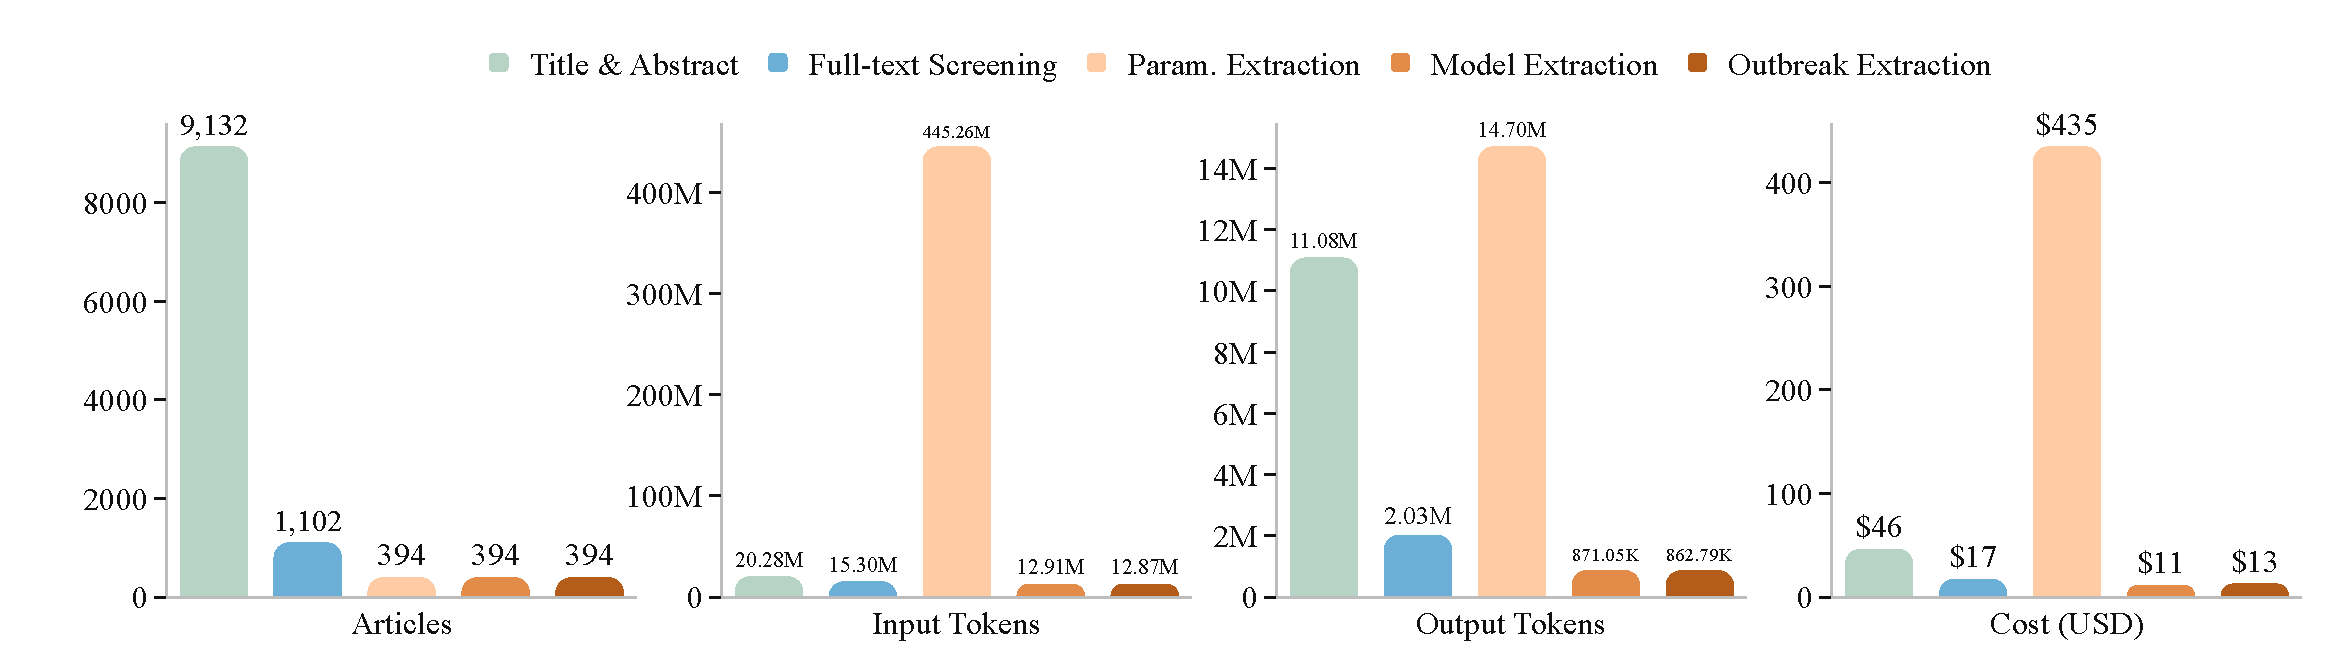
\includegraphics[width=\linewidth]{figures/pipeline_stats/token_articles_cost_by_stage.pdf}
    \caption{
\textbf{Articles processed, scaled token and costs by pipeline stage across models.}
We report the average number of articles reaching each stage, and the corresponding total input tokens, output tokens, and USD cost per stage averaged across models. Token totals are computed by multiplying per article token usage (Table~\ref{tab:token_usage_by_stage}) by the average article counts per stage (Table~\ref{tab:perg_slr_article_counts}).
Parameter extraction dominates overall compute, with substantially higher input and output token totals than other stages.
Title and abstract screening processes the largest volume of articles but contributes comparatively less to total cost.
}
    \label{fig:tokens_costs_articles_split}
\end{figure*}


Using the average article counts reported in Table~\ref{tab:perg_slr_article_counts}, we estimate total token usage and USD cost
across pipeline stages by combining per-article token statistics with model-specific
pricing. Figure~\ref{fig:tokens_costs_articles_split} summarises the resulting
distribution of articles processed, aggregate input tokens, output tokens, and total
cost by stage, averaged across models. Per-article input and output token usage by
stage and model is reported in Table~\ref{tab:token_usage_by_stage}. Total stage costs
are computed by multiplying mean per-article token usage by the average number of
articles reaching each stage, and then applying published per-million-token pricing
for both input and output tokens. All prices used in these calculations are retrieved
directly from the primary API pricing documentation of each model provider at the time
of evaluation.
Under this pricing regime, parameter extraction dominates overall compute and cost due
to substantially higher input and output token volumes, while title and abstract
screening processes the largest number of articles but contributes comparatively
little to total cost. All reported costs reflect managed API usage; alternative cost
estimates could be derived for deployments hosted on dedicated GPU nodes, where pricing
would depend on hardware configuration, utilisation, and amortisation assumptions
rather than per-token billing.

\footnotetext{
\textbf{GPT-OSS-120B:} \url{https://openrouter.ai/openai/gpt-oss-120b}. \\
\textbf{GPT-5.2:} \url{https://developers.openai.com/api/docs/pricing/}. \\
\textbf{DeepSeek-V3.2:} \url{https://api-docs.deepseek.com/quick_start/pricing}. \\
\textbf{Kimi-K2.5:} \url{https://platform.moonshot.ai/docs/pricing/chat}. \\
\textbf{GLM-4.7:} \url{https://docs.z.ai/guides/overview/pricing}.
}

% \SP{A) Mention in main-text the estimated costs are based on OpenRouter B) [Optional] Compute costs if self-hosted open-source models}



\begin{table*}[h]
\centering
\caption{
\textbf{Per article token usage and estimated cost by stage and model.}
We report mean input tokens, output tokens, and USD cost for processing a \textbf{single article} at each stage.
\highP{Green} marks the minimum and \lowP{Red} marks the maximum within each row and subcolumn.
}
\label{tab:token_usage_by_stage}
\setlength{\tabcolsep}{1.3pt}
\renewcommand{\arraystretch}{1.2}
{\footnotesize
\begin{tabular}{l|ccc|ccc|ccc|ccc|ccc}
\toprule
\textbf{Stage} & \multicolumn{3}{c|}{\textbf{GPT-OSS-120B (High)}} & \multicolumn{3}{c|}{\textbf{GPT-5.2 (High)}} & \multicolumn{3}{c|}{\textbf{DeepSeek-V3.2}} & \multicolumn{3}{c|}{\textbf{Kimi-K2.5}} & \multicolumn{3}{c}{\textbf{GLM-4.7}} \\
 & \makecell[c]{Input\\Tok.} & \makecell[c]{Output\\Tok.} & \makecell[c]{Cost\\(USD)} & \makecell[c]{Input\\Tok.} & \makecell[c]{Output\\Tok.} & \makecell[c]{Cost\\(USD)} & \makecell[c]{Input\\Tok.} & \makecell[c]{Output\\Tok.} & \makecell[c]{Cost\\(USD)} & \makecell[c]{Input\\Tok.} & \makecell[c]{Output\\Tok.} & \makecell[c]{Cost\\(USD)} & \makecell[c]{Input\\Tok.} & \makecell[c]{Output\\Tok.} & \makecell[c]{Cost\\(USD)} \\
\midrule
\makecell[l]{Title \& Abstract\\Screening} & \lowP{2.3K} & 1.2K& \highP{$<0.01$} & 2.2K& \highP{0.6K} & \lowP{0.01} & \highP{2.2K} & 0.6K& $<0.01$ & 2.3K& \lowP{2.0K} & $<0.01$ & 2.2K& 1.6K& $<0.01$ \\
\midrule
\makecell[l]{Article Screening\\(AI Conditioned)} & \lowP{16.9K} & 1.1K& \highP{$<0.01$} & 13.1K& 1.4K& \lowP{0.04} & \highP{12.9K} & \highP{0.8K} & $<0.01$ & 13.1K& 2.7K& 0.01 & 13.4K& \lowP{3.1K} & 0.01 \\
\midrule
\makecell[l]{Parameter\\Extraction} & \highP{510.2K} & 19.8K& \highP{0.02} & 961.1K& \lowP{91.1K} & \lowP{2.95} & 523.2K& \highP{3.0K} & 0.14 & 605.5K& 40.0K& 0.48 & \lowP{3050.4K} & 32.7K& 1.90 \\
\midrule
\makecell[l]{Model\\Extraction} & 35.9K& 1.9K& \highP{$<0.01$} & 31.5K& 2.1K& \lowP{0.08} & \lowP{37.2K} & \lowP{3.1K} & 0.01 & \highP{29.3K} & 2.2K& 0.02 & 29.7K& \highP{1.7K} & 0.02 \\
\midrule
\makecell[l]{Outbreak\\Extraction} & \lowP{49.9K} & 2.6K& \highP{$<0.01$} & 32.4K& \lowP{3.5K} & \lowP{0.10} & 26.1K& \highP{0.2K} & $<0.01$ & 29.5K& 2.7K& 0.02 & \highP{25.4K} & 2.0K& 0.01 \\
\midrule
\textbf{Overall} & 615.3K& 26.7K& \highP{0.02} & 1040.4K& \lowP{98.7K} & \lowP{3.20} & \highP{601.6K} & \highP{7.8K} & 0.17 & 679.8K& 49.6K& 0.55 & \lowP{3121.1K} & 41.1K& 1.96 \\
\bottomrule
\end{tabular}
}
\end{table*}
% \begin{itemize}
%     \item https://openrouter.ai/openai/gpt-oss-120b
%     \item https://platform.moonshot.ai/docs/pricing
%     \item https://developers.openai.com/api/docs/pricing/
%     \item https://docs.z.ai/guides/overview/pricing
%     \tem https://api-docs.deepseek.com/quick_start/pricing
% \end{itemize}

% PRICE_IN  = {'GPT-OSS-120B (High)':0.039,'GPT-5.2 (High)':1.75,'DeepSeek-V3.2':0.28,'Kimi-K2.5':0.6,'GLM-4.7':0.6}
% PRICE_OUT = {'GPT-OSS-120B (High)':0.19,'GPT-5.2 (High)':14.0,'DeepSeek-V3.2':0.42,'Kimi-K2.5':3.0,'GLM-4.7':2.2}





\clearpage


\clearpage
\section{Extended  Results}\label{app:pipeline_stage_eval}
This section reports disaggregated results across pathogens and stages for \name{} (\texttt{gpt-oss-120b}), presented in \cref{sec:PERG_data_evaluation}.

\subsection{Article Screening}
\label{app:extended_results_article_screening}

\subsubsection*{Title and Abstract Screening}
Table~\ref{tab:abstract_screening_metrics} summarises title-and-abstract screening performance across seven pathogens, showing moderate overall recall ($0.72$) alongside high precision ($0.79$), for an overall $F_1$ of $0.74$. This pattern suggests the abstract-stage screening is tuned toward specificity, prioritising the rejection of irrelevant studies at the cost of more false negatives. Performance is broadly consistent across pathogens, with the strongest balance for MERS ($F_1$ of $0.78$) and the weakest for Marburg ($F_1$ of $0.69$).


\begin{table}[h]
\centering
\caption{\textbf{Precision, recall, and $F_1$ for title-and-abstract screening across seven pathogens with \name{} (\texttt{gpt-oss-120b}).} Metrics summarise how well the abstract-stage classifier retained studies judged relevant under PERG screening criteria, reported for each pathogen and overall. Overall performance (precision $0.79$, recall $0.72$; $F_1$ $0.74$) reflects a specificity-oriented triage step that prioritises avoiding false inclusions, with lower recall indicating that some relevant studies may require recovery at the full-text stage. $P=\text{precision}$; $R=\text{recall}$; $F_1=\text{F1-Score}$.}
\label{tab:abstract_screening_metrics}
\renewcommand{\arraystretch}{1}
\setlength{\tabcolsep}{8pt}
{\footnotesize
\begin{tabular}{l|ccc}
\toprule
\textbf{Pathogen} & $P$ & $R$ & $F_1$ \\
\midrule
Marburg & 0.80 & 0.64 & 0.69 \\
Ebola & 0.74 & 0.75 & 0.75 \\
Lassa & 0.82 & 0.72 & 0.75 \\
SARS & 0.78 & 0.76 & 0.77 \\
Zika & 0.73 & 0.77 & 0.75 \\
MERS & 0.83 & 0.74 & 0.78 \\
Nipah & 0.84 & 0.66 & 0.70 \\
\midrule
Overall & 0.79 & 0.72 & 0.74 \\
\bottomrule
\end{tabular}
}
\end{table}



\subsubsection*{Full-text Screening}
Table~\ref{tab:fulltext_screening_metrics} compares three full-text screening strategies and highlights a clear precision–recall trade-off. Human abstract $\rightarrow$ AI full-text achieves the strongest overall performance (precision $0.83$, recall $0.92$), while the fully automated two-stage pipeline (AI abstract $\rightarrow$ AI full-text) shows lower recall ($0.81$), consistent with error propagation from abstract gating. Direct AI full-text screening improves recall ($0.89$) but reduces precision ($0.68$), reflecting a recall-maximising approach when abstracts are treated as an information bottleneck.

\begin{table}[h]
\centering
\caption{\textbf{Full-text screening performance on \name{} (\texttt{gpt-oss-120b}) under three operational strategies for identifying relevant articles.} Metrics compare a two-stage AI pipeline (AI abstract$\rightarrow$AI full-text), a mixed workflow (human abstract$\rightarrow$AI full-text), and direct AI full-text screening, reported for each pathogen and overall. Results show the trade-off between recall preservation and precision control: human abstract gating yields the highest overall $F_1$ score ($0.87$), while direct AI full-text maximises recall ($0.89$) at the cost of precision ($0.68$), consistent with abstracts acting as an information bottleneck. $P=\text{precision}$; $R=\text{recall}$; $F_1=\text{F1-Score}$.}
\footnotesize
\label{tab:fulltext_screening_metrics}
\renewcommand{\arraystretch}{1}
\setlength{\tabcolsep}{6pt}
{\footnotesize
\begin{tabular}{l|ccc|ccc|ccc}
\toprule
\multirow{2}{*}{\textbf{Pathogen}}
& \multicolumn{3}{c|}{\makecell{\textbf{AI Screen (Abstract)}\\$\rightarrow$\\\textbf{AI Screen (Full-text)}}}
& \multicolumn{3}{c|}{\makecell{\textbf{Human Screen (Abstract)}\\$\rightarrow$\\\textbf{AI Screen (Full-text)}}}
& \multicolumn{3}{c}{\makecell{~\\\textbf{AI Screen (Direct Full-text)}\\~}} \\
\cline{2-10}
\rule{0pt}{9pt}
& $P$ & $R$ & $F_1$
& $P$ & $R$ & $F_1$
& $P$ & $R$ & $F_1$ \\
\midrule
Marburg & 0.75 & 0.76 & 0.75 & 0.77 & 0.83 & 0.80 & 0.64 & 0.82 & 0.69 \\
Ebola & 0.73 & 0.84 & 0.77 & 0.86 & 0.97 & 0.91 & 0.67 & 0.93 & 0.72 \\
Lassa & 0.79 & 0.78 & 0.78 & 0.83 & 0.94 & 0.88 & 0.71 & 0.91 & 0.77 \\
SARS & 0.71 & 0.85 & 0.76 & 0.80 & 0.95 & 0.86 & 0.64 & 0.91 & 0.68 \\
Zika & 0.66 & 0.79 & 0.69 & 0.81 & 0.91 & 0.85 & 0.64 & 0.85 & 0.67 \\
MERS & 0.76 & 0.83 & 0.79 & 0.83 & 0.96 & 0.88 & 0.69 & 0.95 & 0.76 \\
Nipah & 0.87 & 0.84 & 0.85 & 0.89 & 0.90 & 0.90 & 0.74 & 0.88 & 0.79 \\
\midrule
Overall & 0.75 & 0.81 & 0.77 & 0.83 & 0.92 & 0.87 & 0.68 & 0.89 & 0.73 \\
\bottomrule
\end{tabular}
}
\end{table}


\clearpage












\subsection{Data Extraction}\label{app:data_extraction_extended}
In this section, we provide complete disaggregated results for our data extraction evaluations comparing \name{} extractions against our ground-truth-labelled datasets. The ground-truth-labelled datasets are provided open-source from the Pathogen Epidemiology Review Group, available through the R \texttt{epireview} package or on GitHub at \href{https://github.com/mrc-ide/epireview/tree/main/inst/extdata}{https://github.com/mrc-ide/epireview/tree/main/inst/extdata}.

As of March 2026, owing to PERG's continual progress through SLRs on nine priority pathogens, ground-truth extraction data is available in a standardised format for four pathogens: Lassa, Ebola, SARS, and Zika. For each pathogen, we evaluate classification measures for each of the \textit{Flagging}, \textit{Count}, and \textit{Extraction} metrics defined formally in \Cref{app:data_extraction_extended_methods}.

\subsubsection*{Parameters}

\Cref{tab:parameters_extended_flagging_count} presents the results for parameter extraction Flagging and Count metrics. These results are used to produce the aggregate data presented in the main body text (\Cref{tab:data_extraction_metrics} in \Cref{sec:pipeline_experimental_results}). For flagging relevant parameters, \name{} performs consistently across all pathogens with high recall ($0.92$ average), though precision is lower and more variable ($0.51$ average). The results suggest that while \name{} is able to identify nearly all relevant extractions, this coverage comes at the cost of many false positive flags that may propagate errors to later sub-stages. In terms of overall parameter extraction counts, the performance flips in favour of precision ($0.83$) now at the expense of lower recall ($0.47$). The discrepancy with parameter flagging performance is understandable, as \name{} is capable of disregarding flagged parameters when provided with the option for structured extraction via tool calls. Our data suggests that when \name{} produces a final extraction, this extraction is likely correct, however the system often fails to produce all required extractions according to ground-truth data. An article may have multiple extractions of the same parameter class, and in these cases \name{} can underestimate the number of extractions required.

\begin{table}[h]

\centering
\caption{\textbf{Flagging and Count classification metrics for parameter extraction with \name{} (\texttt{gpt-oss-120b}).} $P=\text{precision}$; $R=\text{recall}$; $F_1=\text{F1-Score}$.}
\label{tab:parameters_extended_flagging_count}
\renewcommand{\arraystretch}{1}
{\footnotesize
\begin{tabular}{l|cccccccccccc}
\toprule
\bf Metric & \multicolumn{3}{c}{\textbf{Lassa}} & \multicolumn{3}{c}{\textbf{Ebola}} & \multicolumn{3}{c}{\textbf{SARS}} & \multicolumn{3}{c}{\textbf{Zika}} \\
 & $P$ & $R$ & $F_1$ & $P$ & $R$ & $F_1$ & $P$ & $R$ & $F_1$ & $P$ & $R$ & $F_1$ \\
\midrule
\bf Flagging & 0.56 &
0.98 &
0.71 &
0.60 &
0.92 &
0.72 &
0.50 &
0.81 &
0.62 &
0.40 &
0.96 &
0.57 \\
\midrule
\bf Count & 1.00 &
0.35 &
0.51 &
0.79 &
0.47 &
0.59 &
0.80 &
0.61 &
0.69 &
0.72 &
0.47 &
0.57 \\
\bottomrule
\end{tabular}
}
\end{table}


\begin{table}[h]
\setlength{\tabcolsep}{3pt}
\centering
\caption{\textbf{Field-level precision, recall, and $F_1$ for Extraction on parameters with \name{} (\texttt{gpt-oss-120b}).} \textit{Group} corresponds to the sub-stage of parameter extraction where the field is collected. The final row shows averages across all fields. $P=\text{precision}$; $R=\text{recall}$; $F_1=\text{F1-Score}$.}
\label{tab:parameters_detailed_metrics}
\renewcommand{\arraystretch}{1}
{\footnotesize
\begin{tabular}{ll|ccc|ccc|ccc|ccc}
\toprule
\bf Group & \bf Field & \multicolumn{3}{c}{\textbf{Lassa}} & \multicolumn{3}{c}{\textbf{Ebola}} & \multicolumn{3}{c}{\textbf{SARS}} & \multicolumn{3}{c}{\textbf{Zika}} \\
 & & $P$ & $R$ & $F_1$ & $P$ & $R$ & $F_1$ & $P$ & $R$ & $F_1$ & $P$ & $R$ & $F_1$ \\
\midrule
\multirow{4}{*}{\textbf{Value}} & value & 0.22 & 0.22 & 0.22 & 0.20 & 0.20 & 0.20 & 0.23 & 0.23 & 0.23 & 0.14 & 0.14 & 0.14 \\
 & unit & 0.50 & 0.43 & 0.46 & 0.62 & 0.35 & 0.44 & 0.69 & 0.61 & 0.65 & 0.65 & 0.43 & 0.52 \\
 & method & 1.00 & 0.89 & 0.94 & 0.48 & 0.78 & 0.59 & 0.76 & 0.83 & 0.79 & 0.86 & 0.80 & 0.83 \\
\cmidrule{2-14}
 & Average & 0.57 & 0.51 & 0.54 & 0.44 & 0.44 & 0.41 & 0.56 & 0.56 & 0.56 & 0.55 & 0.46 & 0.50 \\
\midrule
\multirow{5}{*}{\textbf{Uncertainty}} & value type & 0.38 & 0.43 & 0.40 & 0.30 & 0.33 & 0.32 & 0.35 & 0.57 & 0.43 & 0.12 & 0.22 & 0.16 \\
 & statistical approach & -- & -- & -- & -- & -- & -- & -- & -- & -- & 0.44 & 0.66 & 0.53 \\
 & single type uncertainty & 1.00 & 1.00 & 1.00 & 0.98 & 0.94 & 0.96 & 0.81 & 0.95 & 0.88 & 0.97 & 0.99 & 0.98 \\
 & paired uncertainty & 0.25 & 0.40 & 0.31 & 0.59 & 0.72 & 0.65 & 0.39 & 0.88 & 0.54 & 0.46 & 0.90 & 0.61 \\
\cmidrule{2-14}
 & Average & 0.54 & 0.61 & 0.57 & 0.62 & 0.67 & 0.64 & 0.52 & 0.80 & 0.62 & 0.50 & 0.69 & 0.57 \\
\midrule
\multirow{4}{*}{\textbf{Population}} & population sex & 0.86 & 0.67 & 0.75 & 0.62 & 0.79 & 0.69 & 0.59 & 0.75 & 0.66 & 0.59 & 0.70 & 0.64 \\
 & population group & 0.14 & 0.11 & 0.12 & 0.24 & 0.33 & 0.28 & 0.23 & 0.25 & 0.24 & 0.54 & 0.54 & 0.54 \\
 & population sample type & 0.86 & 0.67 & 0.75 & 0.32 & 0.41 & 0.36 & 0.58 & 0.63 & 0.60 & 0.37 & 0.36 & 0.37 \\
\cmidrule{2-14}
 & Average & 0.62 & 0.48 & 0.54 & 0.40 & 0.51 & 0.44 & 0.47 & 0.54 & 0.50 & 0.50 & 0.54 & 0.52 \\
\midrule
\textbf{Overall} & & 0.58 & 0.53 & 0.55 & 0.49 & 0.54 & 0.50 & 0.51 & 0.63 & 0.56 & 0.51 & 0.57 & 0.53 \\
\bottomrule
\end{tabular}
}
\end{table}

For Extraction, complete field-level results are presented in \Cref{tab:parameters_detailed_metrics}. The aggregate results, presented in the main text, show parameter extractions to have moderate quality across all pathogens, with little variation among them. Analysing the results at the field-level reveals patterns in \name{}'s handling of different data modalities as well as different types of epidemiological context. The system performs worst on value fields, with population fields also showing relatively weak performance, compared to other groups. We suspect the difficulty with population context arises from the large numbers of valid options for many fields (notably population group and population sample type), with many of these options having precise interpretations in epidemiological literature. Without fine-tuning, \texttt{gpt-oss-120b} may struggle to apply these interpretations in a complex tool-calling environment. On the other hand, classification is near perfect for single type uncertainty, and generally strong for method (with the exception of Ebola). We also note that fields with unrestricted domains, like value, are much harder to classify correctly. Seeing the much improved results in our expert validation experiment (\Cref{sec:human_expert_validation}), we suspect at least some of this difficulty to stem from our exact-match criteria being overly punitive of equivalent numbers in different formats.


\subsubsection*{Transmission Models}
\Cref{tab:models_detailed_metrics} presents the complete results for Flagging, Count, and Extraction evaluations of transmission models across the four priority pathogens. Screening performance was strong across all pathogens for article flagging, with recall ranging from $0.86$ to $0.99$ and precision from $0.86$ to $0.96$, indicating reliable identification of modelling studies. Model count extraction achieved consistently high recall ($0.97$--$1.00$) but notably lower precision ($0.48$--$0.60$), suggesting a systematic tendency to overestimate the number of models reported per article rather than failing to identify them.


\begin{table}[b!]
\setlength{\tabcolsep}{3pt}
\centering
\caption{\textbf{Precision, recall, and $F_1$ metrics for transmission model screening and extraction across four pathogens with \name{} (\texttt{gpt-oss-120b}).} \textit{Screening} includes article flagging and model count accuracy. \textit{Extraction} evaluates field-level accuracy for matched model pairs, covering core structural characteristics (model type, stochastic vs deterministic, theoretical vs data-fitted, code availability) and more complex multi-value fields (transmission routes, assumptions, interventions). Strong performance is observed for core model characteristics, while extraction of assumptions, interventions, and transmission routes remains more challenging. $P=\text{precision}$; $R=\text{recall}$; $F_1=\text{F1-Score}$.}
\label{tab:models_detailed_metrics}
\renewcommand{\arraystretch}{1}
{\footnotesize
\begin{tabular}{l|cccccccccccc}
\toprule
 & \multicolumn{3}{c}{\textbf{Lassa}} & \multicolumn{3}{c}{\textbf{Ebola}} & \multicolumn{3}{c}{\textbf{SARS}} & \multicolumn{3}{c}{\textbf{Zika}} \\
 & $P$ & $R$ & $F1$ & $P$ & $R$ & $F1$ & $P$ & $R$ & $F1$ & $P$ & $R$ & $F1$ \\
\midrule
\multicolumn{13}{l}{\textbf{Flagging}} \\
Article Flagging
& 0.95 & 0.99 & 0.97
& 0.92 & 0.92 & 0.92
& 0.86 & 0.86 & 0.86
& 0.87 & 0.89 & 0.88 \\
\midrule
\multicolumn{13}{l}{\textbf{Counts}} \\
Model Count
& 0.60 & 1.00 & 0.75
& 0.50 & 1.00 & 0.67
& 0.49 & 0.97 & 0.65
& 0.48 & 0.98 & 0.65 \\
\midrule
\multicolumn{13}{l}{\textbf{Extraction}} \\
Model Type
& 0.89 & 0.89 & 0.89
& 0.89 & 0.89 & 0.89
& 0.77 & 0.77 & 0.77
& 0.88 & 0.88 & 0.88 \\
\midrule
Compartmental Type
& 0.00 & 0.00 & 0.00
& --- & --- & ---
& 0.80 & 0.80 & 0.80
& 0.83 & 0.83 & 0.83 \\
\midrule
Stochastic vs Deterministic
& 1.00 & 1.00 & 1.00
& 0.75 & 0.85 & 0.80
& 0.76 & 0.78 & 0.77
& 0.82 & 0.79 & 0.81 \\
\midrule
Theoretical vs Data-Fitted
& 0.78 & 0.78 & 0.78
& 0.88 & 0.88 & 0.88
& 0.62 & 0.62 & 0.62
& 0.81 & 0.81 & 0.81 \\
\midrule
Code Available
& 1.00 & 0.89 & 0.94
& 0.85 & 0.84 & 0.84
& 1.00 & 1.00 & 1.00
& 0.82 & 0.76 & 0.79 \\
\midrule
Transmission Routes
& 1.00 & 0.94 & 0.97
& 0.13 & 0.15 & 0.14
& 0.26 & 0.32 & 0.29
& 0.68 & 0.74 & 0.71 \\
\midrule
Assumptions
& 0.29 & 0.46 & 0.36
& 0.27 & 0.46 & 0.34
& 0.21 & 0.39 & 0.28
& 0.31 & 0.52 & 0.39 \\
\midrule
Interventions
& 0.54 & 0.64 & 0.58
& 0.48 & 0.69 & 0.56
& 0.46 & 0.79 & 0.58
& 0.32 & 0.69 & 0.43 \\
\midrule
\textbf{Overall}
& 0.70 & 0.78 & 0.73
& 0.62 & 0.77 & 0.67
& 0.61 & 0.75 & 0.66
& 0.66 & 0.81 & 0.71 \\
\bottomrule
\end{tabular}
}
\end{table}

Field-level extraction showed a clear gradient in task difficulty. Core structural characteristics were extracted with high accuracy: model type classification and the theoretical versus data-fitted distinction achieved balanced precision and recall between $0.62$ and $0.89$ across pathogens, while single-value fields such as stochastic versus deterministic modelling and code availability frequently exceeded $0.75$ and reached perfect scores for some pathogens. In contrast, more complex or multi-value fields exhibited substantially lower performance. Transmission route extraction was particularly challenging for Ebola and SARS, while assumptions and interventions showed modest precision and recall across all pathogens. Overall, across screening and extraction tasks, precision ranged from $0.61$ to $0.70$ and recall from $0.75$ to $0.81$, indicating that the system reliably captures core model characteristics, with remaining limitations concentrated in the extraction of nuanced descriptive details.




\subsubsection*{Outbreaks}


\begin{table}[t!]
\centering
\caption{\textbf{Precision, recall, and $F_1$ for outbreak screening and extraction with \name{} (\texttt{gpt-oss-120b}) across major feature categories, evaluated against expert-curated PERG database.} \textit{Screening} measured article flagging (identifying papers containing outbreaks) and outbreak count accuracy (extracting the correct number of outbreaks per paper). \textit{Extraction} evaluated field-level accuracy for matched outbreak pairs across four epidemiological categories: temporal features (start/end dates), geographic features (country, specific location), case burden (confirmed cases, deaths), and epidemiological context (detection mode, pre-outbreak status, ongoing status, asymptomatic transmission). Overall metrics represent the average across all extraction fields. $P=\text{precision}$; $R=\text{recall}$; $F_1=\text{F1-Score}$.}
\renewcommand{\arraystretch}{1}
{\footnotesize
\label{tab:outbreak_aggregated_metrics}
\begin{tabular}{ll|ccc|ccc}
\toprule
 \multirow{2}{*}{\bf Metric} & \multirow{2}{*}{\bf Field}
 & \multicolumn{3}{c}{\textbf{Lassa}}
 & \multicolumn{3}{c}{\textbf{Zika}} \\
 & & $P$ & $R$ & $F1$ & $P$ & $R$ & $F1$ \\
\midrule
\bf Flagging & Article Flagging & 0.69 & 0.82 & 0.75 & 0.58 & 0.71 & 0.64 \\
\midrule
\bf Counts & Outbreak Counts & 0.83 & 1.00 & 0.91 & 0.49 & 0.45 & 0.47 \\
\midrule
\multirow{4}{*}{\textbf{Extraction}} & Temporal Features & 0.83 & 0.74 & 0.78 & 0.85 & 0.82 & 0.83 \\
 & Geographic and Spatial Features & 0.75 & 0.78 & 0.76 & 0.75 & 0.75 & 0.75 \\
 & Case Burden & 0.82 & 0.75 & 0.79 & 0.93 & 0.93 & 0.93 \\
 & Epidemiological Context and Metadata & 0.93 & 0.70 & 0.80 & 0.84 & 0.67 & 0.75 \\
\midrule
\textbf{Overall} &  & 0.85 & 0.73 & 0.79 & 0.84 & 0.78 & 0.81 \\
\bottomrule
\end{tabular}
}
\end{table}

\begin{table}[b!]
\centering
\caption{\textbf{Detailed (expanded) precision, recall, and $F_1$ for outbreak feature extraction by category for \name{} (\texttt{gpt-oss-120b}).} Each row shows field-level performance within the four major epidemiological categories. Temporal and case burden features showed consistently high performance, while location-specific fields and epidemiological context features showed greater variability. Overall metrics represent the average across all 13 extraction fields. $P=\text{precision}$; $R=\text{recall}$; $F_1=\text{F1-Score}$.}
\label{tab:outbreak_detailed_metrics}
\renewcommand{\arraystretch}{1}
{\footnotesize
\begin{tabular}{l|cccccc}
\toprule
 & \multicolumn{3}{c}{\textbf{Lassa}} & \multicolumn{3}{c}{\textbf{Zika}} \\
 & $P$ & $R$ & $F1$ & $P$ & $R$ & $F1$ \\
\midrule
\multicolumn{7}{l}{\textbf{Temporal Features}} \\
Start Year & 0.89 & 0.80 & 0.84 & 0.90 & 0.82 & 0.86 \\
Start Month & 0.78 & 0.78 & 0.78 & 0.80 & 0.80 & 0.80 \\
Start Day & 0.86 & 0.67 & 0.75 & 0.95 & 0.95 & 0.95 \\
End Month & 0.78 & 0.78 & 0.78 & 0.65 & 0.65 & 0.65 \\
End Day & 0.86 & 0.67 & 0.75 & 0.95 & 0.86 & 0.90 \\
\textbf{Average} & 0.83 & 0.74 & 0.78 & 0.85 & 0.82 & 0.83 \\
\midrule
\multicolumn{7}{l}{\textbf{Geographic and Spatial Features}} \\
Outbreak Country & 1.00 & 1.00 & 1.00 & 1.00 & 1.00 & 1.00 \\
Location & 0.50 & 0.56 & 0.53 & 0.50 & 0.50 & 0.50 \\
\textbf{Average} & 0.75 & 0.78 & 0.77 & 0.75 & 0.75 & 0.75 \\
\midrule
\multicolumn{7}{l}{\textbf{Case Burden}} \\
Confirmed Cases & 0.75 & 0.60 & 0.67 & 0.86 & 0.86 & 0.86 \\
Deaths & 0.90 & 0.90 & 0.90 & 1.00 & 1.00 & 1.00 \\
\textbf{Average} & 0.83 & 0.75 & 0.79 & 0.93 & 0.93 & 0.93 \\
\midrule
\multicolumn{7}{l}{\textbf{Epidemiological Context and Metadata}} \\
Mode of Detection & 0.71 & 0.50 & 0.59 & 0.50 & 0.41 & 0.45 \\
Pre-outbreak Status & 1.00 & 0.30 & 0.46 & 1.00 & 0.41 & 0.58 \\
Ongoing Status & 1.00 & 1.00 & 1.00 & 0.86 & 0.86 & 0.86 \\
Asymptomatic Transmission & 1.00 & 1.00 & 1.00 & 1.00 & 1.00 & 1.00 \\
\textbf{Average} & 0.93 & 0.70 & 0.76 & 0.84 & 0.67 & 0.72 \\
\midrule
\textbf{Overall} & 0.85 & 0.73 & 0.79 & 0.84 & 0.78 & 0.81 \\
\bottomrule
\end{tabular}
}
\end{table}


Similar to transmission models, applying the evaluation framework described in Appendix~\ref{app:additional_evaluation_details}, we analysed outbreak extraction performance across two priority pathogens, Lassa and Zika (Table~\ref{tab:outbreak_aggregated_metrics}). Screening performance differed between pathogens and screening subtasks. For Lassa, article flagging achieved moderate precision ($0.69$) and strong recall ($0.82$), indicating that most outbreak-containing papers were identified, although a non-trivial fraction of flagged papers were false positives. For Zika, article flagging was more balanced (precision $0.58$, recall $0.71$), suggesting improved sensitivity relative to precision, but still leaving missed outbreak descriptions and over-inclusion of non-outbreak papers. Outbreak counting remained strong for Lassa (precision $0.83$, recall $1.00$), while Zika outbreak counting was substantially lower (precision $0.49$, recall $0.45$), consistent with continued difficulty in reliably enumerating outbreak events in the Zika corpus.


% \newpage
Field-level extraction performance, grouped by epidemiological feature categories, revealed consistent strengths and persistent weaknesses (Table~\ref{tab:outbreak_detailed_metrics}). Temporal features remained robust across both pathogens (Lassa: precision $0.83$, recall $0.74$; Zika: precision $0.85$, recall $0.82$), with high precision for start year ($0.89$) and start day ($0.86$) in Lassa, and strong start day accuracy in Zika (precision $0.95$, recall $0.95$). Case burden metrics showed overall extraction (Lassa: precision $0.83$, recall $0.75$; Zika: precision $0.93$, recall $0.93$), with high accuracy for deaths (Lassa: $0.90$/$0.90$; Zika: $1.00$/$1.00$).

Geographic extraction continued to show a split between coarse and fine granularity. Outbreak country identification was perfect for both pathogens ($1.00$ precision and recall), while specific location extraction was notably weaker (Lassa: precision $0.50$, recall $0.56$; Zika: precision $0.50$, recall $0.50$), consistent with variability in how places are described in scientific text. Epidemiological context fields showed the greatest variability: for Lassa, mode of detection was moderate ($0.71$ precision, $0.50$ recall) and pre-outbreak status exhibited high precision but low recall ($1.00$/$0.30$), indicating frequent omission of this attribute. Ongoing status was extracted perfectly for Lassa ($1.00$/$1.00$) but showed moderate performance for Zika ($0.86$/$0.86$). For Zika, mode of detection ($0.50$/$0.41$) and pre-outbreak status ($1.00$/$0.41$) remained challenging, although asymptomatic transmission was extracted perfectly for both pathogens ($1.00$/$1.00$). The overall extraction performance averaged $0.85$ precision and $0.73$ recall for Lassa, and $0.84$ precision and $0.78$ recall for Zika, suggesting reliable field-level accuracy with remaining gaps concentrated in context-dependent and location-specific attributes.


\clearpage
\clearpage
\section{Model Ablation Results}\label{app:model_ablations}
This section reports full pathogen-level and metric-level results for the five model ablations described in Section~\ref{sec:model_ablations}. 

% Tables~\ref{tab:ta_screening_model_ablation} and~\ref{tab:fulltext_screening_model_ablation} cover the two screening stages, evaluated across seven pathogens (Marburg, Ebola, Lassa, SARS, Zika, MERS, and Nipah). Tables~\ref{tab:parameter_extraction_model_ablation} and~\ref{tab:model_extraction_model_ablation} cover parameter and model extraction respectively, evaluated across four pathogens (Ebola, Lassa, SARS, and Zika). Table~\ref{tab:outbreak_extraction_model_ablation} covers outbreak extraction, evaluated across two pathogens (Lassa and Zika).

\subsection{Article Screening}
\subsubsection*{Title \& Abstract Screening}

At title and abstract screening (Table~\ref{tab:ta_screening_model_ablation}), the spread in overall $F_1$ from $0.62$ (\texttt{DeepSeek-V3.2}) to $0.77$ (\texttt{Kimi-K2.5}) is driven almost entirely by recall rather than precision: \texttt{DeepSeek-V3.2} and GPT-5.2 are the two most precise models ($0.83$ and $0.82$ respectively) yet rank last and fourth on $F_1$, with recalls of $0.59$ and $0.61$ against \texttt{Kimi-K2.5}'s $0.75$. \texttt{Kimi-K2.5} is the best-performing model for all seven pathogens. Nipah is the worst-performing pathogen for three models and sits at or below $0.72$ for all five, consistent with it being one of the smallest and most heterogeneous corpora in the PERG dataset; the same pathogen has the narrowest precision-recall gap across models, suggesting the difficulty is intrinsic to the articles rather than a model-specific calibration issue.


\begin{table*}[h]
\centering
\caption{\textbf{Title and abstract screening metrics with model ablations.} \highP{Green} and \lowP{Red} denote the best- and worst-performing pathogens for each model (in terms of $F_1$ score). \bestM{Bold} indicates the best-performing model for each pathogen, and \secondM{Underline} indicates the second-best. $P=\text{precision}$; $R=\text{recall}$; $F_1=\text{F1-Score}$.}
\label{tab:ta_screening_model_ablation}
\setlength{\tabcolsep}{3pt}
\renewcommand{\arraystretch}{1}
{\footnotesize
\begin{tabular}{l|ccc|ccc|ccc|ccc|ccc}
\toprule
\textbf{Pathogen} & \multicolumn{3}{c|}{\textbf{\texttt{gpt-oss-120b}}} & \multicolumn{3}{c|}{\textbf{GPT-5.2}} & \multicolumn{3}{c|}{\textbf{\texttt{DeepSeek-V3.2}}} & \multicolumn{3}{c|}{\textbf{\texttt{Kimi-K2.5}}} & \multicolumn{3}{c}{\textbf{\texttt{GLM-4.7}}} \\
& $P$ & $R$ & $F1$ & $P$ & $R$ & $F1$ & $P$ & $R$ & $F1$ & $P$ & $R$ & $F1$ & $P$ & $R$ & $F1$ \\
\midrule
\textbf{Marburg} & 0.80 & 0.64 & \lowP{\secondM{0.69}} & 0.97 & 0.58 & 0.62 & 0.97 & 0.55 & 0.58 & 0.79 & 0.65 & \lowP{\bestM{0.69}} & 0.88 & 0.61 & 0.66 \\
\textbf{Ebola} & 0.74 & 0.75 & 0.75 & 0.76 & 0.64 & \highP{0.68} & 0.80 & 0.61 & 0.64 & 0.79 & 0.79 & \bestM{0.79} & 0.88 & 0.72 & \secondM{0.77} \\
\textbf{Lassa} & 0.82 & 0.72 & \secondM{0.75} & 0.78 & 0.63 & 0.66 & 0.84 & 0.60 & 0.63 & 0.84 & 0.77 & \bestM{0.80} & 0.88 & 0.68 & 0.73 \\
\textbf{SARS} & 0.78 & 0.76 & 0.77 & 0.77 & 0.62 & 0.65 & 0.82 & 0.62 & \highP{0.66} & 0.80 & 0.78 & \bestM{0.79} & 0.89 & 0.73 & \highP{\secondM{0.78}} \\
\textbf{Zika} & 0.73 & 0.77 & \secondM{0.75} & 0.70 & 0.62 & 0.64 & 0.73 & 0.63 & 0.66 & 0.78 & 0.79 & \bestM{0.79} & 0.76 & 0.69 & 0.72 \\
\textbf{MERS} & 0.83 & 0.74 & \highP{\secondM{0.78}} & 0.87 & 0.62 & 0.67 & 0.86 & 0.60 & 0.65 & 0.86 & 0.78 & \highP{\bestM{0.81}} & 0.89 & 0.67 & 0.73 \\
\textbf{Nipah} & 0.84 & 0.66 & \secondM{0.70} & 0.92 & 0.58 & \lowP{0.59} & 0.81 & 0.54 & \lowP{0.53} & 0.85 & 0.68 & \bestM{0.72} & 0.90 & 0.61 & \lowP{0.65} \\
\midrule
\textbf{Overall} & 0.79 & 0.72 & \secondM{0.74} & 0.82 & 0.61 & 0.65 & 0.83 & 0.59 & 0.62 & 0.82 & 0.75 & \bestM{0.77} & 0.87 & 0.67 & 0.72 \\
\bottomrule
\end{tabular}
}
\end{table*}

\subsubsection*{Full-text Screening}

The ranking reorders substantially at full-text screening (Table~\ref{tab:fulltext_screening_model_ablation}), where \texttt{gpt-oss-120b} leads ($F_1$ $0.77$) and the two highest-precision abstract-stage models fall furthest. \texttt{DeepSeek-V3.2}'s precision drops from $0.83$ to $0.64$ and its recall from $0.59$ to $0.56$, making it the only model that loses ground on both measures simultaneously, with its Marburg result ($F_1$ $0.42$, precision $0.37$) being the single weakest pathogen-level score in either screening table. \texttt{gpt-oss-120b}'s advantage at this stage comes from recall: it achieves $0.81$ overall against the next-best \texttt{Kimi-K2.5} at $0.73$, and is one of only two models -- alongside \texttt{GLM-4.7} -- for which recall increases from abstract to full-text screening. The Nipah-to-Zika contrast also reverses: Nipah is the best-performing pathogen for \texttt{gpt-oss-120b} and \texttt{Kimi-K2.5} at full-text ($F_1$ $0.85$ and $0.82$), whereas it was the worst for three models at the abstract stage, suggesting that the richer context of full texts resolves ambiguity that titles and abstracts leave open for this pathogen.




\begin{table*}[h]
\centering
\caption{\textbf{Full-text screening metrics with model ablations.}  \highP{Green} and \lowP{Red} denote the best- and worst-performing pathogens for each model (in terms of $F_1$ score). \bestM{Bold} indicates the best-performing model for each pathogen, and \secondM{Underline} indicates the second-best. $P=\text{precision}$; $R=\text{recall}$; $F_1=\text{F1-Score}$.}
\label{tab:fulltext_screening_model_ablation}
\footnotesize
\setlength{\tabcolsep}{3pt}
\renewcommand{\arraystretch}{1}
{\footnotesize
\begin{tabular}{l|ccc|ccc|ccc|ccc|ccc}
\toprule
\textbf{Pathogen} & \multicolumn{3}{c|}{\textbf{\texttt{gpt-oss-120b}}} & \multicolumn{3}{c|}{\textbf{GPT-5.2}} & \multicolumn{3}{c|}{\textbf{\texttt{DeepSeek-V3.2}}} & \multicolumn{3}{c|}{\textbf{\texttt{Kimi-K2.5}}} & \multicolumn{3}{c}{\textbf{\texttt{GLM-4.7}}} \\
& $P$ & $R$ & $F1$ & $P$ & $R$ & $F1$ & $P$ & $R$ & $F1$ & $P$ & $R$ & $F1$ & $P$ & $R$ & $F1$ \\
\midrule
\textbf{Marburg} & 0.75 & 0.76 & \secondM{0.75} & 0.76 & 0.59 & 0.59 & 0.37 & 0.49 & \lowP{0.42} & 0.66 & 0.66 & 0.66 & 0.86 & 0.72 & \highP{\bestM{0.76}} \\
\textbf{Ebola} & 0.73 & 0.84 & \bestM{0.77} & 0.61 & 0.60 & 0.60 & 0.68 & 0.59 & 0.55 & 0.72 & 0.74 & 0.71 & 0.75 & 0.75 & \secondM{0.75} \\
\textbf{Lassa} & 0.79 & 0.78 & \bestM{0.78} & 0.66 & 0.63 & 0.63 & 0.63 & 0.54 & 0.47 & 0.74 & 0.75 & \secondM{0.74} & 0.77 & 0.73 & 0.73 \\
\textbf{SARS} & 0.71 & 0.85 & \bestM{0.76} & 0.60 & 0.58 & 0.58 & 0.73 & 0.61 & \highP{0.59} & 0.67 & 0.69 & 0.66 & 0.73 & 0.72 & \secondM{0.72} \\
\textbf{Zika} & 0.66 & 0.79 & \lowP{\bestM{0.69}} & 0.50 & 0.50 & \lowP{0.50} & 0.61 & 0.55 & 0.52 & 0.63 & 0.64 & \lowP{\secondM{0.61}} & 0.60 & 0.59 & \lowP{0.59} \\
\textbf{MERS} & 0.76 & 0.83 & \bestM{0.79} & 0.66 & 0.61 & 0.61 & 0.74 & 0.60 & 0.58 & 0.76 & 0.79 & \secondM{0.77} & 0.76 & 0.68 & 0.69 \\
\textbf{Nipah} & 0.87 & 0.84 & \highP{\bestM{0.85}} & 0.80 & 0.63 & \highP{0.63} & 0.73 & 0.56 & 0.53 & 0.83 & 0.81 & \highP{\secondM{0.82}} & 0.72 & 0.61 & 0.61 \\
\midrule
\textbf{Overall} & 0.75 & 0.81 & \bestM{0.77} & 0.66 & 0.59 & 0.59 & 0.64 & 0.56 & 0.52 & 0.72 & 0.73 & \secondM{0.71} & 0.74 & 0.69 & 0.69 \\
\bottomrule
\end{tabular}
}
\end{table*}






\subsection{Data Extraction}
\subsubsection*{Parameters}
Parameter extraction results are disaggregated by pathogen and extraction type in Table~\ref{tab:parameter_extraction_model_ablation}. \texttt{Kimi-K2.5} achieves the highest overall average $F_1$ ($0.63$), marginally ahead of \texttt{GLM-4.7} ($0.63$), and lower performance seen for \texttt{gpt-oss-120b} ($0.59$), GPT-5.2 ($0.58$) and \texttt{DeepSeek-V3.2} ($0.56$). Performance is most variable in the Counts sub-task: \texttt{gpt-oss-120b} attains strong precision ($0.83$) but low recall ($0.47$), reproducing the asymmetric pattern observed for the primary model in Appendix~\ref{app:pipeline_stage_eval}, while GPT-5.2 shows the inverse (recall $0.83$, precision $0.36$). At the field-level Extraction sub-task, GPT-5.2 achieves the highest overall $F_1$ ($0.59$), followed by \texttt{Kimi-K2.5} ($0.56$), and the five models are broadly comparable, consistent with the interpretation that cross-model differences in average $F_1$ are driven by flagging and counting behaviour rather than the quality of individual field extractions. Zika is the weakest pathogen across most models and sub-tasks, while SARS is frequently the best-performing for \texttt{gpt-oss-120b}.


\begin{table*}[h]
\centering
\caption{\textbf{Parameter extraction metrics with model ablations.} \textbf{Average} denotes means across sub-tasks; \textbf{Overall} denotes means across pathogens. \highP{Green} and \lowP{Red} denote the best- and worst-performing pathogens for each model (in terms of $F_1$ score). \bestM{Bold} indicates the best-performing model for each pathogen, and \secondM{Underline} indicates the second-best. $P=\text{precision}$; $R=\text{recall}$; $F_1=\text{F1-Score}$.}
\label{tab:parameter_extraction_model_ablation}
\setlength{\tabcolsep}{3pt}
\renewcommand{\arraystretch}{1}
{\footnotesize
\begin{tabular}{ll|ccc|ccc|ccc|ccc|ccc}
\toprule
\textbf{Pathogen} & \textbf{Type} & \multicolumn{3}{c|}{\textbf{\texttt{gpt-oss-120b}}} & \multicolumn{3}{c|}{\textbf{GPT-5.2}} & \multicolumn{3}{c|}{\textbf{\texttt{DeepSeek-V3.2}}} & \multicolumn{3}{c|}{\textbf{\texttt{Kimi-K2.5}}} & \multicolumn{3}{c}{\textbf{\texttt{GLM-4.7}}} \\
& & $P$ & $R$ & $F1$ & $P$ & $R$ & $F1$ & $P$ & $R$ & $F1$ & $P$ & $R$ & $F1$ & $P$ & $R$ & $F1$ \\
\midrule
\multirow{4}{*}{\textbf{Ebola}} & Flagging & 0.60 & 0.92 & \highP{0.72} & 0.58 & 0.93 & 0.71 & 0.49 & 0.91 & 0.64 & 0.67 & 0.90 & \secondM{0.77} & 0.72 & 0.82 & \bestM{0.77} \\
 & Counts & 0.79 & 0.47 & 0.59 & 0.46 & 0.80 & \highP{0.58} & 0.57 & 0.59 & 0.58 & 0.52 & 0.73 & \secondM{0.61} & 0.59 & 0.65 & \bestM{0.62} \\
 & Extraction & 0.48 & 0.54 & \lowP{0.50} & 0.58 & 0.57 & \bestM{0.57} & 0.54 & 0.47 & 0.49 & 0.55 & 0.57 & \lowP{\secondM{0.55}} & 0.51 & 0.56 & \lowP{0.52} \\
 & Average & 0.62 & 0.64 & 0.60 & 0.54 & 0.77 & 0.62 & 0.54 & 0.65 & 0.57 & 0.58 & 0.73 & \bestM{0.64} & 0.61 & 0.68 & \secondM{0.64} \\
\midrule
\multirow{4}{*}{\textbf{Lassa}} & Flagging & 0.56 & 0.98 & 0.71 & 0.58 & 1.00 & \highP{0.73} & 0.54 & 0.91 & \highP{0.68} & 0.70 & 0.94 & \highP{\secondM{0.81}} & 0.77 & 0.87 & \highP{\bestM{0.82}} \\
 & Counts & 1.00 & 0.35 & \lowP{0.51} & 0.30 & 0.85 & 0.45 & 0.46 & 0.57 & \lowP{0.51} & 0.59 & 0.81 & \highP{\bestM{0.69}} & 0.74 & 0.59 & \highP{\secondM{0.66}} \\
 & Extraction & 0.58 & 0.54 & 0.55 & 0.66 & 0.63 & \highP{\bestM{0.63}} & 0.55 & 0.46 & \lowP{0.47} & 0.58 & 0.60 & \highP{\secondM{0.57}} & 0.58 & 0.56 & \highP{0.56} \\
 & Average & 0.71 & 0.62 & 0.59 & 0.51 & 0.83 & 0.61 & 0.52 & 0.65 & 0.55 & 0.62 & 0.79 & \bestM{0.69} & 0.70 & 0.67 & \secondM{0.68} \\
\midrule
\multirow{4}{*}{\textbf{SARS}} & Flagging & 0.50 & 0.81 & \bestM{0.62} & 0.47 & 0.83 & 0.60 & 0.39 & 0.78 & \lowP{0.52} & 0.56 & 0.69 & \lowP{0.62} & 0.58 & 0.67 & \lowP{\secondM{0.62}} \\
 & Counts & 0.80 & 0.61 & \highP{\bestM{0.69}} & 0.37 & 0.88 & 0.52 & 0.60 & 0.60 & \highP{\secondM{0.60}} & 0.45 & 0.72 & \lowP{0.56} & 0.51 & 0.59 & \lowP{0.55} \\
 & Extraction & 0.51 & 0.63 & \highP{0.56} & 0.56 & 0.63 & \bestM{0.58} & 0.58 & 0.54 & \highP{0.55} & 0.53 & 0.65 & \highP{\secondM{0.57}} & 0.51 & 0.62 & 0.55 \\
 & Average & 0.61 & 0.69 & \bestM{0.62} & 0.47 & 0.78 & 0.57 & 0.52 & 0.64 & 0.56 & 0.51 & 0.69 & \secondM{0.58} & 0.53 & 0.63 & 0.57 \\
\midrule
\multirow{4}{*}{\textbf{Zika}} & Flagging & 0.40 & 0.96 & \lowP{0.57} & 0.43 & 0.95 & \lowP{0.59} & 0.41 & 0.94 & 0.57 & 0.56 & 0.86 & \bestM{0.68} & 0.62 & 0.75 & \secondM{0.68} \\
 & Counts & 0.72 & 0.47 & 0.57 & 0.31 & 0.80 & \lowP{0.45} & 0.50 & 0.60 & 0.55 & 0.55 & 0.73 & \secondM{0.63} & 0.59 & 0.67 & \bestM{0.63} \\
 & Extraction & 0.52 & 0.57 & 0.53 & 0.56 & 0.59 & \lowP{\bestM{0.56}} & 0.55 & 0.50 & 0.51 & 0.54 & 0.59 & \secondM{0.55} & 0.52 & 0.58 & 0.54 \\
 & Average & 0.55 & 0.67 & 0.56 & 0.43 & 0.78 & 0.53 & 0.49 & 0.68 & 0.54 & 0.55 & 0.73 & \bestM{0.62} & 0.58 & 0.66 & \secondM{0.61} \\
\midrule
\multirow{4}{*}{\textbf{Overall}} & Flagging & 0.51 & 0.92 & 0.66 & 0.51 & 0.93 & 0.66 & 0.46 & 0.88 & 0.60 & 0.62 & 0.85 & \secondM{0.72} & 0.67 & 0.78 & \bestM{0.72} \\
 & Counts & 0.83 & 0.47 & 0.59 & 0.36 & 0.83 & 0.50 & 0.53 & 0.59 & 0.56 & 0.53 & 0.75 & \bestM{0.62} & 0.61 & 0.62 & \secondM{0.61} \\
 & Extraction & 0.52 & 0.57 & 0.54 & 0.59 & 0.61 & \bestM{0.59} & 0.56 & 0.49 & 0.50 & 0.55 & 0.60 & \secondM{0.56} & 0.53 & 0.58 & 0.54 \\
 & Average & 0.62 & 0.65 & 0.59 & 0.49 & 0.79 & 0.58 & 0.52 & 0.66 & 0.56 & 0.57 & 0.73 & \bestM{0.63} & 0.60 & 0.66 & \secondM{0.63} \\
\bottomrule
\end{tabular}
}
\end{table*}

\subsubsection*{Transmission Models}
Transmission model extraction results are presented in Table~\ref{tab:model_extraction_model_ablation}. \texttt{GLM-4.7} achieves the highest overall average $F_1$ ($0.85$), with strong performance across all three sub-tasks: Flagging ($0.93$), Counts ($0.93$), and Extraction ($0.68$). \texttt{DeepSeek-V3.2} ranks second overall ($0.81$), driven by notably high Counts performance ($0.92$), whilst \texttt{gpt-oss-120b} ranks last ($0.75$), held back by comparatively low Counts precision ($0.52$ overall). Lassa is the best-performing pathogen for all five models, with \texttt{GLM-4.7} achieving an overall average $F_1$ of $0.91$ for that pathogen alone, including perfect Flagging and Counts scores. SARS is consistently the most challenging pathogen: Flagging $F_1$ ranges from $0.82$ (\texttt{DeepSeek-V3.2}) to $0.87$ (\texttt{Kimi-K2.5}), and Extraction $F_1$ from $0.59$ to $0.66$. These patterns are consistent with the field-level difficulties in transmission route and assumption extraction identified in Appendix~\ref{app:pipeline_stage_eval}.


\clearpage

\begin{table*}[t!]
\centering
\caption{\textbf{Model extraction metrics with model ablations.}  \highP{Green} and \lowP{Red} denote the best- and worst-performing pathogens for each model (in terms of $F_1$ score). \textbf{Average} denotes means across sub-tasks; \textbf{Overall} denotes means across pathogens. \bestM{Bold} indicates the best-performing model for each pathogen, and \secondM{Underline} indicates the second-best. $P=\text{precision}$; $R=\text{recall}$; $F_1=\text{F1-Score}$.}
\label{tab:model_extraction_model_ablation}
\setlength{\tabcolsep}{3pt}
\renewcommand{\arraystretch}{1}
{\footnotesize
\begin{tabular}{ll|ccc|ccc|ccc|ccc|ccc}
\toprule
\textbf{Pathogen} & \textbf{Type} & \multicolumn{3}{c|}{\textbf{\texttt{gpt-oss-120b}}} & \multicolumn{3}{c|}{\textbf{GPT-5.2}} & \multicolumn{3}{c|}{\textbf{\texttt{DeepSeek-V3.2}}} & \multicolumn{3}{c|}{\textbf{\texttt{Kimi-K2.5}}} & \multicolumn{3}{c}{\textbf{\texttt{GLM-4.7}}} \\
& & $P$ & $R$ & $F1$ & $P$ & $R$ & $F1$ & $P$ & $R$ & $F1$ & $P$ & $R$ & $F1$ & $P$ & $R$ & $F1$ \\
\midrule
\multirow{4}{*}{\textbf{Ebola}} & Flagging & 0.92 & 0.92 & 0.92 & 0.89 & 0.90 & 0.89 & 0.87 & 0.86 & 0.86 & 0.93 & 0.93 & \secondM{0.93} & 0.95 & 0.94 & \bestM{0.95} \\
 & Counts & 0.50 & 1.00 & 0.67 & 0.56 & 1.00 & 0.71 & 0.81 & 0.99 & \secondM{0.89} & 0.63 & 0.99 & \lowP{0.77} & 0.88 & 0.99 & \bestM{0.93} \\
 & Extraction & 0.59 & 0.72 & 0.64 & 0.62 & 0.74 & \bestM{0.66} & 0.57 & 0.65 & 0.61 & 0.60 & 0.71 & \lowP{0.64} & 0.62 & 0.71 & \secondM{0.66} \\
 & Average & 0.67 & 0.88 & 0.74 & 0.69 & 0.88 & 0.76 & 0.75 & 0.83 & \secondM{0.79} & 0.72 & 0.88 & 0.78 & 0.81 & 0.88 & \bestM{0.84} \\
\midrule
\multirow{4}{*}{\textbf{Lassa}} & Flagging & 0.95 & 0.99 & \highP{\secondM{0.97}} & 0.95 & 0.99 & \highP{\secondM{0.97}} & 0.96 & 0.85 & 0.89 & 0.95 & 0.99 & \highP{\secondM{0.97}} & 1.00 & 1.00 & \highP{\bestM{1.00}} \\
 & Counts & 0.60 & 1.00 & \highP{0.75} & 0.60 & 1.00 & 0.75 & 1.00 & 1.00 & \highP{\bestM{1.00}} & 0.75 & 1.00 & \highP{\secondM{0.86}} & 1.00 & 1.00 & \highP{\bestM{1.00}} \\
 & Extraction & 0.68 & 0.73 & 0.70 & 0.68 & 0.79 & \highP{0.71} & 0.79 & 0.78 & \highP{\bestM{0.78}} & 0.70 & 0.78 & \highP{0.73} & 0.73 & 0.77 & \highP{\secondM{0.74}} \\
 & Average & 0.74 & 0.91 & 0.81 & 0.74 & 0.92 & 0.81 & 0.92 & 0.88 & \secondM{0.89} & 0.80 & 0.92 & 0.85 & 0.91 & 0.92 & \bestM{0.91} \\
\midrule
\multirow{4}{*}{\textbf{SARS}} & Flagging & 0.86 & 0.86 & \lowP{\secondM{0.86}} & 0.86 & 0.86 & \lowP{\secondM{0.86}} & 0.83 & 0.81 & \lowP{0.82} & 0.87 & 0.87 & \lowP{\bestM{0.87}} & 0.85 & 0.84 & \lowP{0.84} \\
 & Counts & 0.49 & 0.97 & 0.65 & 0.49 & 1.00 & \lowP{0.66} & 0.70 & 1.00 & \lowP{\secondM{0.82}} & 0.67 & 1.00 & 0.81 & 0.76 & 1.00 & \lowP{\bestM{0.86}} \\
 & Extraction & 0.60 & 0.71 & \lowP{\secondM{0.64}} & 0.61 & 0.73 & \lowP{0.64} & 0.55 & 0.64 & \lowP{0.59} & 0.63 & 0.74 & \bestM{0.66} & 0.59 & 0.68 & \lowP{0.62} \\
 & Average & 0.65 & 0.85 & 0.72 & 0.65 & 0.86 & 0.72 & 0.70 & 0.82 & 0.74 & 0.72 & 0.87 & \bestM{0.78} & 0.73 & 0.84 & \secondM{0.77} \\
\midrule
\multirow{4}{*}{\textbf{Zika}} & Flagging & 0.87 & 0.89 & 0.88 & 0.89 & 0.91 & 0.90 & 0.90 & 0.89 & \highP{0.90} & 0.90 & 0.92 & \secondM{0.91} & 0.93 & 0.93 & \bestM{0.93} \\
 & Counts & 0.48 & 0.98 & \lowP{0.65} & 0.61 & 1.00 & \highP{0.76} & 0.97 & 0.97 & \bestM{0.97} & 0.72 & 0.97 & 0.83 & 0.88 & 0.97 & \secondM{0.93} \\
 & Extraction & 0.66 & 0.78 & \highP{0.70} & 0.67 & 0.78 & 0.69 & 0.59 & 0.64 & 0.61 & 0.67 & 0.77 & \secondM{0.70} & 0.69 & 0.76 & \bestM{0.71} \\
 & Average & 0.67 & 0.88 & 0.74 & 0.72 & 0.90 & 0.78 & 0.82 & 0.84 & \secondM{0.83} & 0.76 & 0.89 & 0.81 & 0.83 & 0.89 & \bestM{0.85} \\
\midrule
\multirow{4}{*}{\textbf{Overall}} & Flagging & 0.90 & 0.91 & 0.91 & 0.90 & 0.91 & 0.90 & 0.89 & 0.85 & 0.87 & 0.91 & 0.93 & \secondM{0.92} & 0.93 & 0.93 & \bestM{0.93} \\
 & Counts & 0.52 & 0.99 & 0.68 & 0.56 & 1.00 & 0.72 & 0.87 & 0.99 & \secondM{0.92} & 0.69 & 0.99 & 0.81 & 0.88 & 0.99 & \bestM{0.93} \\
 & Extraction & 0.63 & 0.74 & 0.67 & 0.64 & 0.76 & 0.67 & 0.63 & 0.68 & 0.65 & 0.65 & 0.75 & \bestM{0.68} & 0.66 & 0.73 & \secondM{0.68} \\
 & Average & 0.68 & 0.88 & 0.75 & 0.70 & 0.89 & 0.77 & 0.80 & 0.84 & \secondM{0.81} & 0.75 & 0.89 & 0.81 & 0.82 & 0.88 & \bestM{0.85} \\
\bottomrule
\end{tabular}
}
\end{table*}

\subsubsection*{Outbreaks}

Outbreak extraction results, evaluated across Lassa and Zika, are shown in Table~\ref{tab:outbreak_extraction_model_ablation}. GPT-5.2 achieves the highest overall average $F_1$ ($0.77$), followed closely by \texttt{Kimi-K2.5} ($0.76$), \texttt{DeepSeek-V3.2} ($0.73$), \texttt{GLM-4.7} ($0.72$), and \texttt{gpt-oss-120b} ($0.70$). Results diverge sharply between pathogens. Lassa Counts are strong across all models, ranging from $F_1$ $0.77$ (GPT-5.2) to $0.95$ (\texttt{Kimi-K2.5}), and field-level Extraction is uniformly high ($0.76$ to $0.83$). Zika Counts performance falls substantially for \texttt{gpt-oss-120b} ($F_1$ $0.47$) and \texttt{GLM-4.7} ($0.52$), whilst GPT-5.2 remains comparatively strong ($0.83$). A notable divergence in Flagging is also observed: \texttt{DeepSeek-V3.2} performs weakest on Lassa Flagging ($F_1$ $0.62$) whilst achieving the second-best result on Zika ($0.68$). These per-pathogen contrasts are consistent with the field-level analysis of suspected cases and epidemiological context fields reported in Appendix~\ref{app:pipeline_stage_eval}.

\begin{table*}[h] \centering \caption{\textbf{Outbreak extraction metrics with model ablations.} \textbf{Average} denotes means across sub-tasks; \textbf{Overall} denotes means across pathogens. \highP{Green} and \lowP{Red} denote the best- and worst-performing pathogens for each model (in terms of $F_1$ score). \bestM{Bold} indicates the best-performing model for each pathogen, and \secondM{Underline} indicates the second-best. $P=\text{precision}$; $R=\text{recall}$; $F_1=\text{F1-Score}$.} \label{tab:outbreak_extraction_model_ablation} 
{\footnotesize
\setlength{\tabcolsep}{3pt} \renewcommand{\arraystretch}{1} 
\begin{tabular}{ll|ccc|ccc|ccc|ccc|ccc}
\toprule
\textbf{Pathogen} & \textbf{Type} & \multicolumn{3}{c|}{\textbf{\texttt{gpt-oss-120b}}} & \multicolumn{3}{c|}{\textbf{GPT-5.2}} & \multicolumn{3}{c|}{\textbf{\texttt{DeepSeek-V3.2}}} & \multicolumn{3}{c|}{\textbf{\texttt{Kimi-K2.5}}} & \multicolumn{3}{c}{\textbf{\texttt{GLM-4.7}}} \\
& & $P$ & $R$ & $F1$ & $P$ & $R$ & $F1$ & $P$ & $R$ & $F1$ & $P$ & $R$ & $F1$ & $P$ & $R$ & $F1$ \\
\midrule
\multirow{4}{*}{\textbf{Lassa}} & Flagging & 0.69 & 0.82 & \highP{\secondM{0.70}} & 0.72 & 0.84 & \highP{\bestM{0.74}} & 0.61 & 0.65 & \lowP{0.62} & 0.67 & 0.77 & \highP{0.69} & 0.65 & 0.68 & \lowP{0.66} \\
 & Counts & 0.83 & 1.00 & \highP{0.91} & 0.62 & 1.00 & \lowP{0.77} & 0.83 & 1.00 & \highP{0.91} & 0.90 & 1.00 & \highP{\bestM{0.95}} & 1.00 & 0.86 & \highP{\secondM{0.92}} \\
 & Extraction & 0.85 & 0.73 & \lowP{0.77} & 0.84 & 0.79 & \lowP{\secondM{0.81}} & 0.75 & 0.78 & \highP{0.76} & 0.84 & 0.83 & \highP{\bestM{0.83}} & 0.83 & 0.76 & \highP{0.78} \\
 & Average & 0.79 & 0.85 & \secondM{0.80} & 0.73 & 0.88 & 0.78 & 0.73 & 0.81 & 0.77 & 0.80 & 0.87 & \bestM{0.82} & 0.83 & 0.76 & 0.79 \\
\midrule
\multirow{4}{*}{\textbf{Zika}} & Flagging & 0.58 & 0.71 & \lowP{0.53} & 0.59 & 0.75 & \lowP{0.57} & 0.65 & 0.82 & \highP{\secondM{0.68}} & 0.61 & 0.80 & \lowP{0.59} & 0.67 & 0.87 & \highP{\bestM{0.70}} \\
 & Counts & 0.49 & 0.45 & \lowP{0.47} & 0.76 & 0.92 & \highP{\bestM{0.83}} & 0.68 & 0.61 & \lowP{0.64} & 0.72 & 0.88 & \lowP{\secondM{0.79}} & 0.84 & 0.38 & \lowP{0.52} \\
 & Extraction & 0.84 & 0.78 & \highP{\secondM{0.80}} & 0.88 & 0.87 & \highP{\bestM{0.87}} & 0.69 & 0.81 & \lowP{0.73} & 0.71 & 0.78 & \lowP{0.73} & 0.74 & 0.78 & \lowP{0.76} \\
 & Average & 0.64 & 0.65 & 0.60 & 0.75 & 0.84 & \bestM{0.76} & 0.68 & 0.74 & 0.69 & 0.68 & 0.82 & \secondM{0.70} & 0.75 & 0.68 & 0.66 \\
\midrule
\multirow{4}{*}{\textbf{Overall}} & Flagging & 0.63 & 0.76 & 0.61 & 0.66 & 0.79 & \secondM{0.66} & 0.63 & 0.73 & 0.65 & 0.64 & 0.78 & 0.64 & 0.66 & 0.77 & \bestM{0.68} \\
 & Counts & 0.66 & 0.72 & 0.69 & 0.69 & 0.96 & \secondM{0.80} & 0.76 & 0.80 & 0.78 & 0.81 & 0.94 & \bestM{0.87} & 0.92 & 0.62 & 0.72 \\
 & Extraction & 0.85 & 0.76 & \secondM{0.79} & 0.86 & 0.83 & \bestM{0.84} & 0.72 & 0.79 & 0.75 & 0.78 & 0.81 & 0.78 & 0.78 & 0.77 & 0.77 \\
 & Average & 0.71 & 0.75 & 0.70 & 0.74 & 0.86 & \bestM{0.77} & 0.70 & 0.78 & 0.73 & 0.74 & 0.84 & \secondM{0.76} & 0.79 & 0.72 & 0.72 \\
\bottomrule
\end{tabular}
}
\end{table*}

\clearpage
\clearpage
\section{Living Systematic Reviews with \name{} for 9 Priority Pathogens}\label{app:report_writeup}

Utilising \name{} on the data extracted corpus from previous stages, we generated living reviews for nine WHO priority pathogens: Marburg virus, Ebola virus, Lassa virus, SARS-CoV-1, Zika virus, MERS-CoV, Nipah virus, Rift Valley fever (RVF) virus, and Crimean--Congo haemorrhagic fever (CCHF) virus. Each review comprises two complementary documents (a transmission-modelling review synthesising extracted model characteristics, and an outbreak surveillance review aggregating historical outbreak data) alongside structured datasets and visualisations. While four of these pathogens (Ebola, Lassa, SARS, Zika) have been validated against PERG's expert annotations as described in \cref{sec:human_expert_validation}, the remaining five represent preliminary syntheses for pathogens where PERG's systematic review process has not yet commenced or is in early stages.

Figure~\ref{fig:ebola_reviews} presents excerpts from the Ebola living reviews, illustrating the structure and content of \name{}'s outputs for a validated pathogen. The transmission-modelling review (Figure~\ref{fig:ebola_models}) provides a quantitative overview of the $513$ extracted models, including distributions across model architectures, stochasticity classifications, and code availability. The outbreak surveillance review (Figure~\ref{fig:ebola_outbreaks}) synthesises $1,104$ outbreak records spanning nearly six decades, with temporal coverage, geographic distribution, and detection methodology patterns presented through evidence-based descriptions paired with interpretive commentary blocks.

\begin{figure}[h]
    \centering
    \begin{subfigure}[t]{0.6\textwidth}
        \centering
        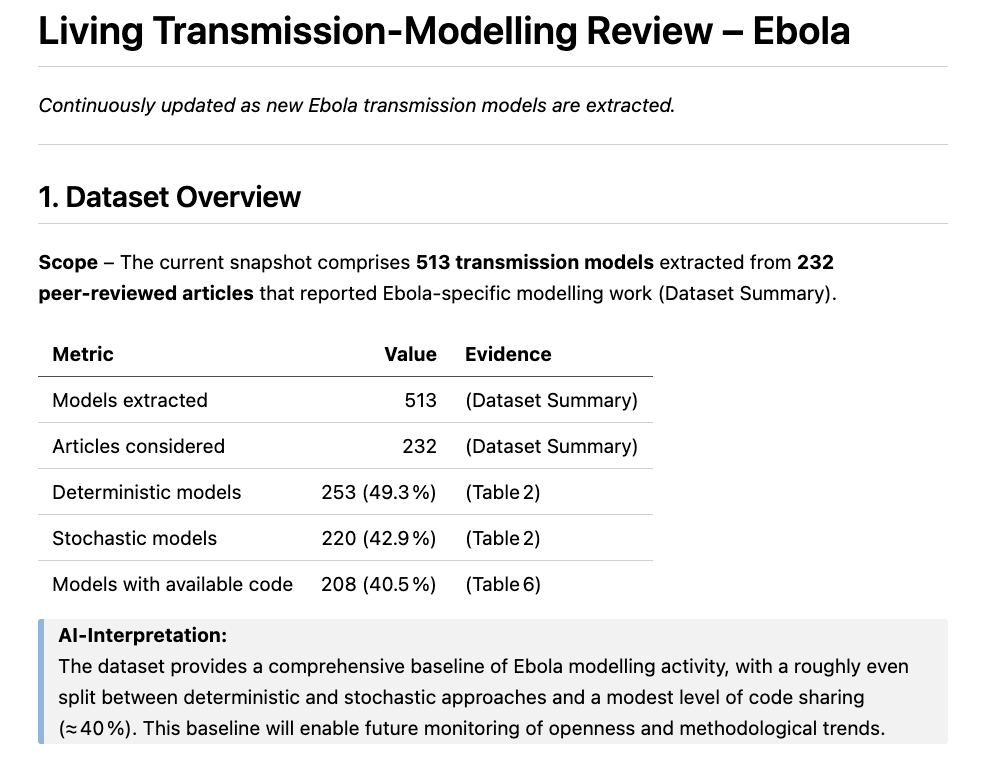
\includegraphics[width=0.6\textwidth]{figures/report_generation/EBOLA_MODELS.png}
        \caption{Transmission-Modelling Review excerpt showing dataset scope, model architecture distribution, and reproducibility indicators for $513$ Ebola models extracted from $232$ articles.}
        \label{fig:ebola_models}
    \end{subfigure}

    \vspace{0.5em} % optional spacing between figures

    \begin{subfigure}[t]{0.6\textwidth}
        \centering
        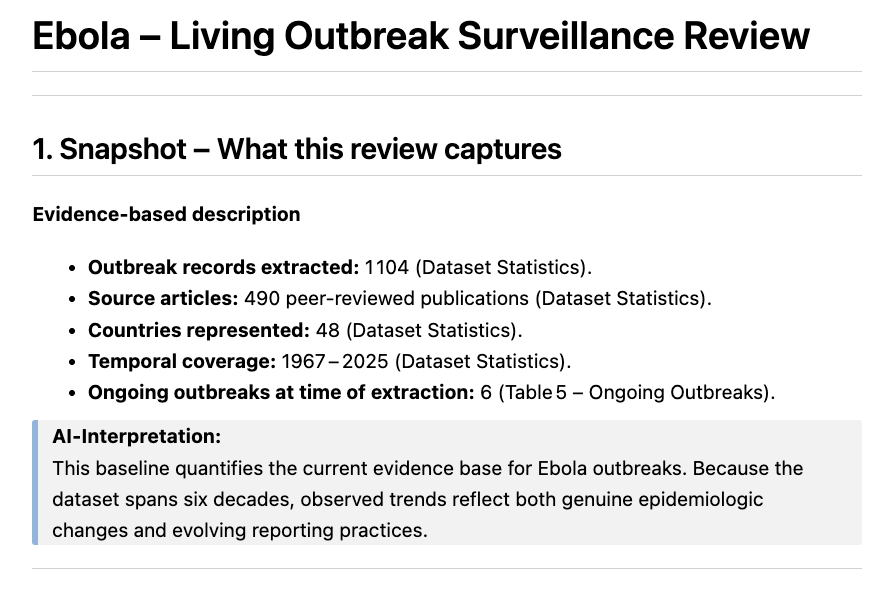
\includegraphics[width=0.6\textwidth]{figures/report_generation/EBOLA_OUTBREAKS.png}
        \caption{Outbreak Surveillance Review excerpt presenting snapshot statistics for $1,104$ outbreak records from $490$ publications, covering temporal span 1967--2025 and $48$ countries.}
        \label{fig:ebola_outbreaks}
    \end{subfigure}

    \caption{\textbf{Ebola living reviews generated by \name{}.} Both reviews follow a structured format: evidence-based descriptions citing supporting figures and tables, followed by interpretation blocks explicitly labelled as AI-generated synthesis. Ebola represents one of four pathogens validated against PERG expert annotations (\cref{sec:human_expert_validation}).}
    \label{fig:ebola_reviews}
\end{figure}
For emerging or understudied pathogens, rapid synthesis of available evidence can inform outbreak preparedness even when comprehensive expert review remains infeasible. Figure~\ref{fig:unvalidated_reviews} presents excerpts from RVF and CCHF reviews, two pathogens for which PERG has not yet initiated systematic screening. The RVF transmission-modelling review (Figure~\ref{fig:rvf_models}) characterises $115$ models extracted from the retrieved literature, revealing a predominance of compartmental architectures and vector-to-human transmission pathways consistent with RVF's arboviral ecology. The CCHF outbreak surveillance review (Figure~\ref{fig:cchf_outbreaks}) maps $59$ outbreak records with quantitative case data, identifying geographic clusters and temporal patterns across affected regions. While these syntheses lack the validation rigour applied to Ebola, Lassa, SARS, and Zika, they demonstrate \name{}'s capacity to generate preliminary evidence summaries for resource allocation and hypothesis generation in under $48$ hours of wall-clock time.

\begin{figure}[h]
    \centering
    \begin{subfigure}[t]{0.48\textwidth}
        \centering
        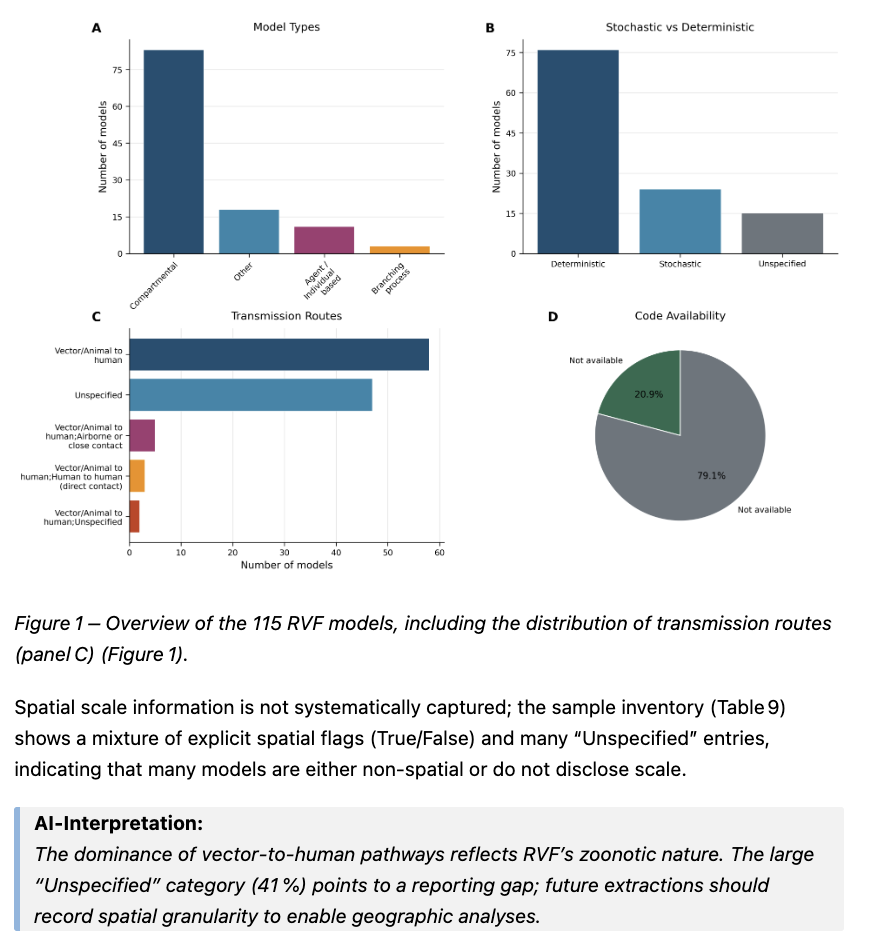
\includegraphics[width=\textwidth]{figures/report_generation/RVF.png}
        \caption{RVF transmission-modelling review showing distribution of $115$ extracted models across architecture types, stochasticity, transmission routes, and code availability.}
        \label{fig:rvf_models}
    \end{subfigure}
    \hfill
    \begin{subfigure}[t]{0.48\textwidth}
        \centering
        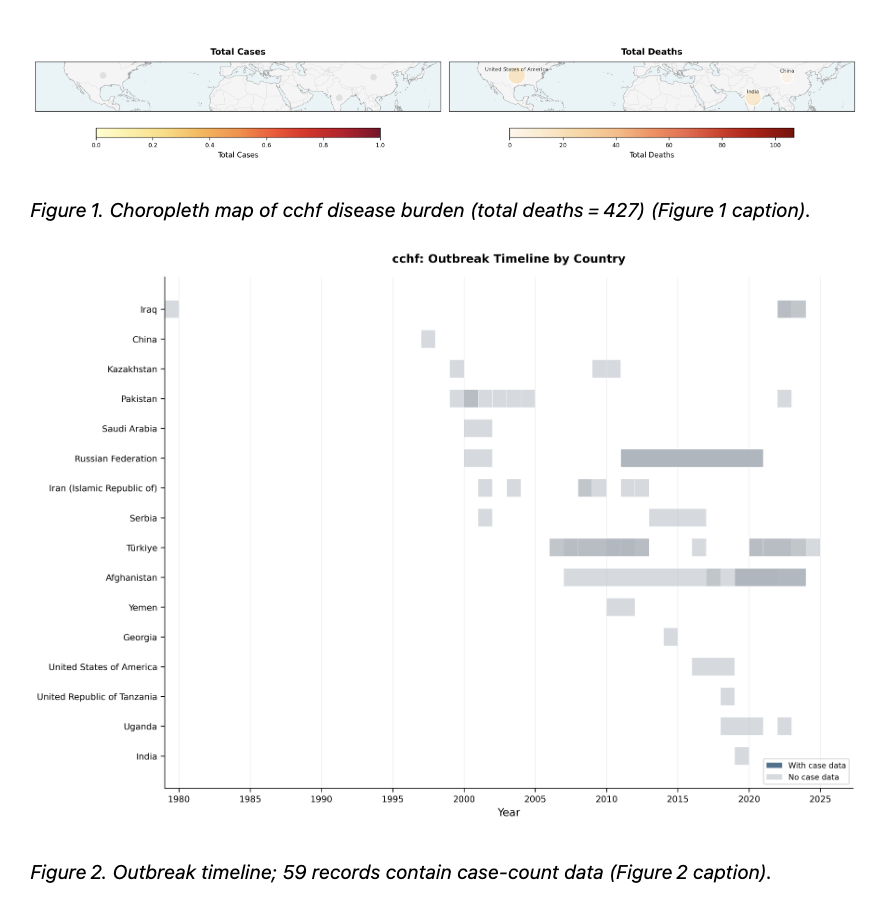
\includegraphics[width=\textwidth]{figures/report_generation/CCHF.png}
        \caption{CCHF outbreak surveillance review presenting geographic burden (choropleth maps) and temporal distribution of $59$ outbreaks with case-count data.}
        \label{fig:cchf_outbreaks}
    \end{subfigure}
    \caption{\textbf{Preliminary living reviews for pathogens without completed PERG validation.} RVF and CCHF represent pathogens for which PERG has not yet commenced systematic screening. These \name{}-generated reviews provide initial evidence synthesis for outbreak preparedness planning, though they lack the expert validation applied to the four evaluated pathogens (Ebola, Lassa, SARS, Zika).}
    \label{fig:unvalidated_reviews}
\end{figure}


Table~\ref{tab:review_contents} summarises the standardised artefact structure maintained across all pathogen reviews. Both transmission-modelling and outbreak surveillance reports follow consistent schemas: model reviews characterise architecture distributions, stochasticity classifications, transmission pathways, and reproducibility indicators, whilst outbreak reviews present temporal timelines, geographic burden maps, detection methodology breakdowns, and case-count summaries. This structural consistency enables direct cross-pathogen comparison and ensures that future updates (as literature accumulates or as PERG completes validation for additional pathogens) maintain compatibility with existing syntheses.

\begin{table}[h]
\centering
\caption{\textbf{Key artefacts in \name{} living reviews.} Each pathogen generates two review types with consistent visualisation and evidence table structures. The text-based LLM  uses manifests, with summary statistics of the figures to write its interpretation.}
\label{tab:review_contents}
\small
\begin{tabular}{lp{0.38\linewidth}p{0.38\linewidth}}
\toprule
\textbf{Type} & \textbf{Transmission-Modelling Review} & \textbf{Outbreak Surveillance Review} \\
\midrule
\textbf{Figures} & 
Model architecture distribution (compartmental, branching process, agent-based); Stochasticity classification; Transmission route breakdown; Code availability 
& 
Geographic burden (choropleth maps for cases and deaths); Outbreak timeline by country; Detection mode distribution \\
\midrule
\textbf{Tables} & 
Model type counts and proportions; Deterministic vs stochastic breakdown; Transmission routes with sample sizes; Modelling assumptions; Intervention categories; Spatial scale indicators; Code availability and language 
& 
Outbreak source categories; Detection methodology breakdown; Ongoing outbreaks at extraction; Case burden stratified by confirmation status; Sex disaggregation where reported \\
\bottomrule
\end{tabular}
\end{table}

\clearpage

\clearpage
\section{Extended Expert Validation Results}

Six epidemiology researchers contributed to our validation survey. We collected $62$ submissions for parameters, $50$ for models, and $31$ for outbreaks. \Cref{tab:expert_validation_results} reports all metrics collected from the survey. The main text reports the aggregate statistics (the ‘Overall’ rows for each data type) in the first two columns columns of \Cref{fig:expert_validation_results}.

% \begin{figure}[H]
%     \centering
%     \caption{\textbf{Full expert-rated flagging precision and extraction accuracy results by parameter class and extraction field.}}
%     \label{fig:extended_validation_results}
%     \includegraphics[width=\linewidth]{figures/results/expert_survey_extended.pdf}
% \end{figure}



{\footnotesize
\begin{longtable}{>{\raggedright\arraybackslash}p{10.8cm} S[table-format=1.2, round-mode=places, round-precision=2]}
\caption{\textbf{Extended expert validation results.} Results are reported as expert-rated flagging precision and expert-rated extraction accuracy. Within each section, rows are ordered from overall scores to subgroup scores and then field-level scores.}
\label{tab:expert_validation_results} \\
\toprule
\textbf{Item} & {\textbf{Score}} \\
\midrule
\endfirsthead

\multicolumn{2}{l}{\textit{Table \thetable\ continued from previous page}} \\
\toprule
\textbf{Item} & {\textbf{Score}} \\
\midrule
\endhead

\midrule
\multicolumn{2}{r}{\textit{Continued on next page}} \\
\endfoot

\bottomrule
\endlastfoot

\multicolumn{2}{l}{\textbf{Parameters}} \\
\addlinespace[0.2em]
Overall --- Flagging precision & 0.66 \\
Overall --- Extraction accuracy & 0.77 \\

\addlinespace[0.35em]
\textit{Precision by class} & {} \\
\quad Attack rate & 0.25 \\
\quad Growth rate & 1.00 \\
\quad Human delay & 0.62 \\
\quad Reproduction number & 1.00 \\
\quad Seroprevalence & 0.50 \\
\quad Severity & 0.57 \\

\addlinespace[0.35em]
\textit{Accuracy by group} & {} \\
\quad Value & 0.89 \\
\quad Uncertainty & 0.76 \\
\quad Population & 0.59 \\
\quad Aggregation & 0.83 \\

\addlinespace[0.35em]
\textit{Value fields} & {} \\
\quad Value & 0.81 \\
\quad Unit & 0.96 \\
\quad Type & 0.88 \\
\quad Bounds & 0.79 \\
\quad Value type & 0.90 \\
\quad Statistical approach & 0.97 \\

\addlinespace[0.35em]
\textit{Uncertainty fields} & {} \\
\quad Single-type uncertainty & 0.88 \\
\quad Paired uncertainty & 0.84 \\
\quad Distribution type & 0.57 \\

\addlinespace[0.35em]
\textit{Population fields} & {} \\
\quad Sample type & 0.74 \\
\quad Population group & 0.49 \\
\quad Sample size & 0.66 \\
\quad Sex & 0.50 \\
\quad Age range & 0.58 \\
\quad Countries & 0.82 \\
\quad Locations & 0.71 \\
\quad Method moment value & 0.23 \\

\addlinespace[0.35em]
\textit{Aggregation fields} & {} \\
\quad Aggregation & 0.83 \\

\addlinespace[0.6em]
\multicolumn{2}{l}{\textbf{Models}} \\
\addlinespace[0.2em]
Overall --- Flagging precision & 0.40 \\
Overall --- Extraction accuracy & 0.83 \\

\addlinespace[0.35em]
\textit{Field accuracy} & {} \\
\quad Model type & 0.89 \\
\quad Compartmental type & 0.89 \\
\quad Stochastic or deterministic & 0.70 \\
\quad Theoretical model & 0.84 \\

\addlinespace[0.6em]
\multicolumn{2}{l}{\textbf{Outbreaks}} \\
\addlinespace[0.2em]
Overall --- Flagging precision & 0.61 \\
Overall --- Extraction accuracy & 0.80 \\

\addlinespace[0.35em]
\textit{Accuracy by group} & {} \\
\quad Temporal & 0.62 \\
\quad Geographical & 0.87 \\
\quad Case burden & 0.85 \\
\quad Epidemiological & 0.85 \\

\addlinespace[0.35em]
\textit{Temporal fields} & {} \\
\quad Start year & 0.84 \\
\quad Start month & 0.70 \\
\quad Start day & 0.62 \\
\quad End year & 0.50 \\
\quad End month & 0.60 \\
\quad End day & 0.56 \\
\quad Duration in months & 0.50 \\

\addlinespace[0.35em]
\textit{Geographical fields} & {} \\
\quad Country & 0.95 \\
\quad Location & 0.80 \\

\addlinespace[0.35em]
\textit{Case burden fields} & {} \\
\quad Confirmed cases & 0.88 \\
\quad Suspected cases & 0.64 \\
\quad Asymptomatic cases & 1.00 \\
\quad Severe cases & 1.00 \\
\quad Deaths & 0.71 \\

\addlinespace[0.35em]
\textit{Epidemiological fields} & {} \\
\quad Mode of detection & 0.82 \\
\quad Pre-outbreak status & 0.82 \\
\quad Asymptomatic transmission described & 0.89 \\

\end{longtable}
}

For flagging (sub-task) precision, models and outbreaks are reported only at the overall level (as in the main text). For parameters, precision is averaged over flagging decisions made for each parameter class. The random subsample of articles assigned gave six relevant parameter classes: attack rate, growth rate, human delay, reproduction number, seroprevalence, and severity. The remaining two parameter classes, mutation rate and relative contribution, were absent from the sample. Since there is a flagging decision made for each parameter class on each article, each parameter class-level precision is calculated over the same sample size ($N=62$).

For extraction accuracy, the aggregate statistics are normalised over groups of similar fields. For example, outbreaks have clusters of fields related to temporal features (start date, end date, and duration), geographical features (country and location), case burden (case counts and fatalities) and epidemiological factors (mode of detection, status pre-outbreak, and asymptomatic transmission). We normalise at the group level to treat each aspect of the extraction as equally important, in order to avoid overemphasising groups with larger numbers of metadata fields. We omit group-level normalisation for models owing to the smaller number of validated fields.

The disaggregated statistics reveal findings that are masked in the average statistics. For example, among parameter classes, \name{} performs worst on flagging attack rate (experts reported several instances where the system confused attack rate with seroprevalence information). At the field level, \name{} struggles the most with understanding parameter population context and with the temporal outbreak features (group accuracy $0.62$). Parameter population fields are multiple-choice selections with many options (see \Cref{tab:population_tool_call}), and these designations often have specific interpretations in epidemiology. For example, ``persons under investigation'' is a population group of patients exhibiting clinical and epidemiological risk factors, a definition that an LLM may struggle to apply consistently in different article contexts.

\clearpage
\section{The PERG Review Pipeline (Human Reference Workflow)}
\label{app:perg_pipeline}

The \emph{Pathogen Epidemiology Review Group (PERG)} is an expert-led effort (started in 2019) whose goal is to maintain a definitive, curated source of epidemiological parameters for pathogens prioritised for epidemic preparedness. In practice, PERG delivers this through systematic literature reviews and meta-analyses targeting the WHO priority pathogens, with the explicit aim of supporting outbreak response and modelling when time is short and parameter choices matter. 

The scope is defined by the WHO priority pathogens framing: diseases that ``pose the greatest public health risk due to their epidemic potential and/or whether there is no or insufficient countermeasures." Examples highlighted in PERG onboarding include CCHF virus, Ebola virus, Marburg virus, Lassa virus, Middle East respiratory syndrome coronavirus (MERS-CoV), Severe Acute Respiratory Syndrome coronavirus 1 (SARS-CoV-1), Nipah virus, Rift Valley fever, and Zika virus. 

PERG’s workflow is end-to-end: it starts from a protocolised literature search, then moves through screening (title \& abstract, then full text), structured extraction into REDCap (including quality-assessment fields guided by the PERG wiki), meta-analysis, and finally the write-up of a review that can be used by modellers and public health teams. 

\subsection*{Step 1: Paper search (protocol-driven, pathogen-specific)}
PERG begins from a registered systematic review protocol (PROSPERO ID:  CRD42023393345), and uses a standardised query template that is then tailored to each pathogen. The core idea is to search broadly across the epidemiological concepts that tend to matter during outbreak response: transmission and epidemiology terms, transmission modelling (with explicit exclusion of imaging-related “model” matches), severity outcomes (e.g. CFR), key delays (e.g. incubation period, serial interval, generation time), transmission heterogeneity and superspreading/overdispersion, transmissibility measures (e.g. growth rate and reproduction numbers), serology/serosurveys, evolutionary signals (mutation/substitution/evolution), outbreak/cluster terminology and risk factors. The query is written with wildcards to capture term variants, and then adjusted where needed to avoid cross-contamination with neighbouring literatures (for example, excluding SARS-CoV-2 when the target is SARS-CoV-1).

% \begin{lstlisting}[basicstyle=\small\ttfamily, breaklines=true, backgroundcolor=\color{gray!10}]
% pathogen AND ((transmissi* OR epidemiolog*) 
% OR (model* NOT imag*) 
% OR ("severity" OR "case fatality ratio*" OR "CFR" OR "case fatality rate*" 
%     OR "mortality rate$" OR "attack rate$") 
% OR ("infectious period" OR "serial interval*" OR "incubation period*" 
%     OR "generation time*" OR "generation interval*" OR "latent period" OR "latency") 
% OR ("heterogeneit*" OR "superspread*" OR "super spread*" OR "super-spread*" OR "overdispers*") 
% OR ("infectivity" OR "infectiousness" OR "growth rate*" OR "reproduction number$" 
%     OR "reproductive number$" OR "R0" OR "reproduction ratio" OR "reproductive rate") 
% OR ("pre-existing immunity" OR "serological" OR "serology" OR "serosurvey*") 
% OR ("evolution*" OR "mutation$" OR "substitution$") 
% OR (outbreak$ OR cluster$ OR epidemic$) 
% OR ("risk factor*"))
% \end{lstlisting}

\subsection*{Step 2: Title and abstract screening (broad triage against explicit criteria)}
The first screening pass is based on titles and abstracts. The emphasis here is not on perfect specificity, but on ensuring the pool remains wide enough to avoid missing relevant evidence that is only clearly described later in the paper. PERG’s \textbf{inclusion criteria} are simple but concrete: studies must be English-language, peer-reviewed original research (systematic reviews and meta-analyses are flagged rather than treated as primary extraction targets), and must involve human data. A paper is kept if it contains \emph{any one} of several types of useful information, including: quantitative descriptions of a human outbreak (size, year, location, duration, spatial scale), a mathematical or statistical model of transmission, estimates of key transmission or timing quantities (e.g., $R$, $R_0$, $R_t$, growth rate, generation time, serial interval, incubation or latent period, other delays), severity metrics (CFR, attack rate), evolutionary rates, overdispersion/superspreading, risk factors (together with the measure), seroprevalence, relative contributions of human-to-human vs zoonotic transmission, and, where relevant, vector-related quantities such as mosquito delays or mosquito reproduction numbers.

PERG’s \textbf{exclusion criteria} are equally explicit: non-English items; posters, conference proceedings, correspondence, and abstract-only records; in-vitro-only studies; solely animal studies (unless the paper provides clearly relevant transmission quantities); and small case studies with fewer than 10 cases.

\subsection*{Step 3: Full-text review (confirm ``extractability")}
Articles passing abstract screening move to full-text review. PERG applies the same conceptual criteria, but with a different mindset: reviewers scan the entire paper to confirm that there is \emph{something extractable}, i.e. not just that the topic is on-target. Importantly, PERG explicitly runs both title and abstract screening and this stage with \textbf{two reviewers}, reflecting the goal of consistency and defensible inclusion decisions when judgement calls are required.

\subsection*{Step 4: Parameter extraction (read, highlight, enter structured fields)}
Once a paper is included, PERG's extraction process is deliberately hands-on. Reviewers (i) check which papers they have been assigned, (ii) download and read the PDF, highlighting everything they may want to extract as they go, and then (iii) enter the extracted information into a REDCap web database (PERG maintains pathogen-specific REDCap projects).

PERG structures extraction into four broad blocks:
\vspace{-10pt}
\begin{itemize}[leftmargin=*, itemsep=-3pt]
    \item  \textit{Article metadata.} Basic bibliographic information such as title, DOI, journal, and related identifiers are recorded. 
    \item  \textit{What the paper contains:} outbreaks, models, parameters. PERG extracts (i) outbreak descriptions where present, (ii) mathematical models of transmission (these are not limited to SIR-type models; they can be theoretical and not necessarily fitted to data), and (iii) epidemiological parameter estimates. Parameter families include genomic/evolutionary quantities (mutation/evolution rates), reproduction numbers ($R_0$, $R_t$, and human-only or vector-related variants where relevant), human delays (serial interval, incubation period, time-to-death, etc.), severity (CFR/IFR), seroprevalence (e.g. IgG/IgM markers), risk factors (with attention to whether effects are statistically significant and adjusted), relative contributions (human-to-human vs animal-to-human), attack rates (including secondary attack rates), and overdispersion (e.g. the negative binomial $k$ parameter). 
    \item \textit{Associated context for interpretation.} PERG captures the contextual details that make parameter estimates comparable (or not): sex (male/female/both/unspecified), sample size, setting (general population vs hospital), subgroup (children, pregnant, etc.), age ranges, country and more specific location, study start/end dates, and whether the study was conducted before/mid/after an outbreak.
    \item \textit{Structured outbreak fields (when applicable)}. In addition to “is there an outbreak?”, PERG-style extraction treats outbreaks as structured entities. In our draft’s PERG-aligned outbreak guidance, outbreak characteristics include temporal bounds (start/end day/month/year; whether ongoing), geographic scope (country plus sub-location), outbreak source, mode of detection, case definition method, case counts by confirmation status (confirmed/probable/suspected/unspecified), asymptomatic and severe cases when reported, deaths, and (when available) demographic breakdown such as sex-disaggregated counts. A key principle is that these values are extracted \emph{as stated in the paper}, without calculating missing quantities or inferring unreported fields.
\end{itemize}


Across all extraction types, PERG points reviewers to the PERG wiki for “how to extract this specific thing” guidance, so that extraction decisions remain consistent across pathogens and across reviewers.

%\subsection*{Step 5: Quality assessment (QA) recorded alongside extraction}
%QA is recorded alongside extraction, using a small set of standard questions with parameter-specific guidance in the wiki. The QA questions are organised around three themes. First, \emph{is the methodological/statistical approach suitable?} (Q1: is it clear and reproducible; Q2: is it robust and appropriate for the stated aim). Second, \emph{are the assumptions and inputs appropriate?} (Q3: clear and reproducible; Q4: justified). Third, \emph{are the data appropriate for the chosen approach, and are data issues handled well?} (Q5: clearly described and reproducible; Q6: issues clearly discussed/acknowledged; Q7: issues accounted for in the methodological approach).

\subsection*{Step 5: Meta-analysis}
After extraction and quality assessment, PERG moves into synthesis and reporting. PERG maintains shared tooling for priority pathogens, including codebases that step through cleaning the extracted database, transforming quantities into a common format where needed, performing meta-analysis, and producing plots and summary tables. These outputs feed directly into the final PERG systematic review and meta-analysis write-up.

\subsection*{Step 6: Write-up}
The final stage is to turn the extracted REDCap database and the meta-analysis outputs into a PERG review that can be used in practice. In PERG, meta-analysis is implemented through shared, pathogen-focused tooling (the \texttt{priority-pathogens} and \texttt{epireview} codebases), which steps through cleaning and transforming the extracted data, running the statistical synthesis, and producing the figures and summary tables. These tables and plots then provide the backbone of the manuscript: the review documents what evidence was found for each parameter family (and in what contexts), presents the quantitative summaries produced by the meta-analysis, and translates them into a curated resource for outbreak modelling and public health decision-making. In PERG’s framing, this write-up is not just a paper draft: it is the mechanism by which extracted parameters become a stable, citable reference for the WHO priority pathogens, with the longer-term aim of supporting an evolving “live” resource as evidence accumulates.


% \begin{figure}[h]
%     \centering
%     \includegraphics[width=0.5\linewidth]{figures/fig1i.png}
%     \caption{\textbf{PERG pipeline:} image PLACEHOLDER}
%     \label{fig:data_extraction_flowchart}
% \end{figure}

\clearpage
\section{\name{} Annotation Tool (Beta)}
\label{appendix:annotation_tool}
This section documents the \name{} annotation and validation interface, a beta-stage prototype designed to facilitate systematic literature reviews (SLRs) through the integration of LLM-assisted information extraction and expert-led verification. 

\begin{figure}[h]
    \centering
    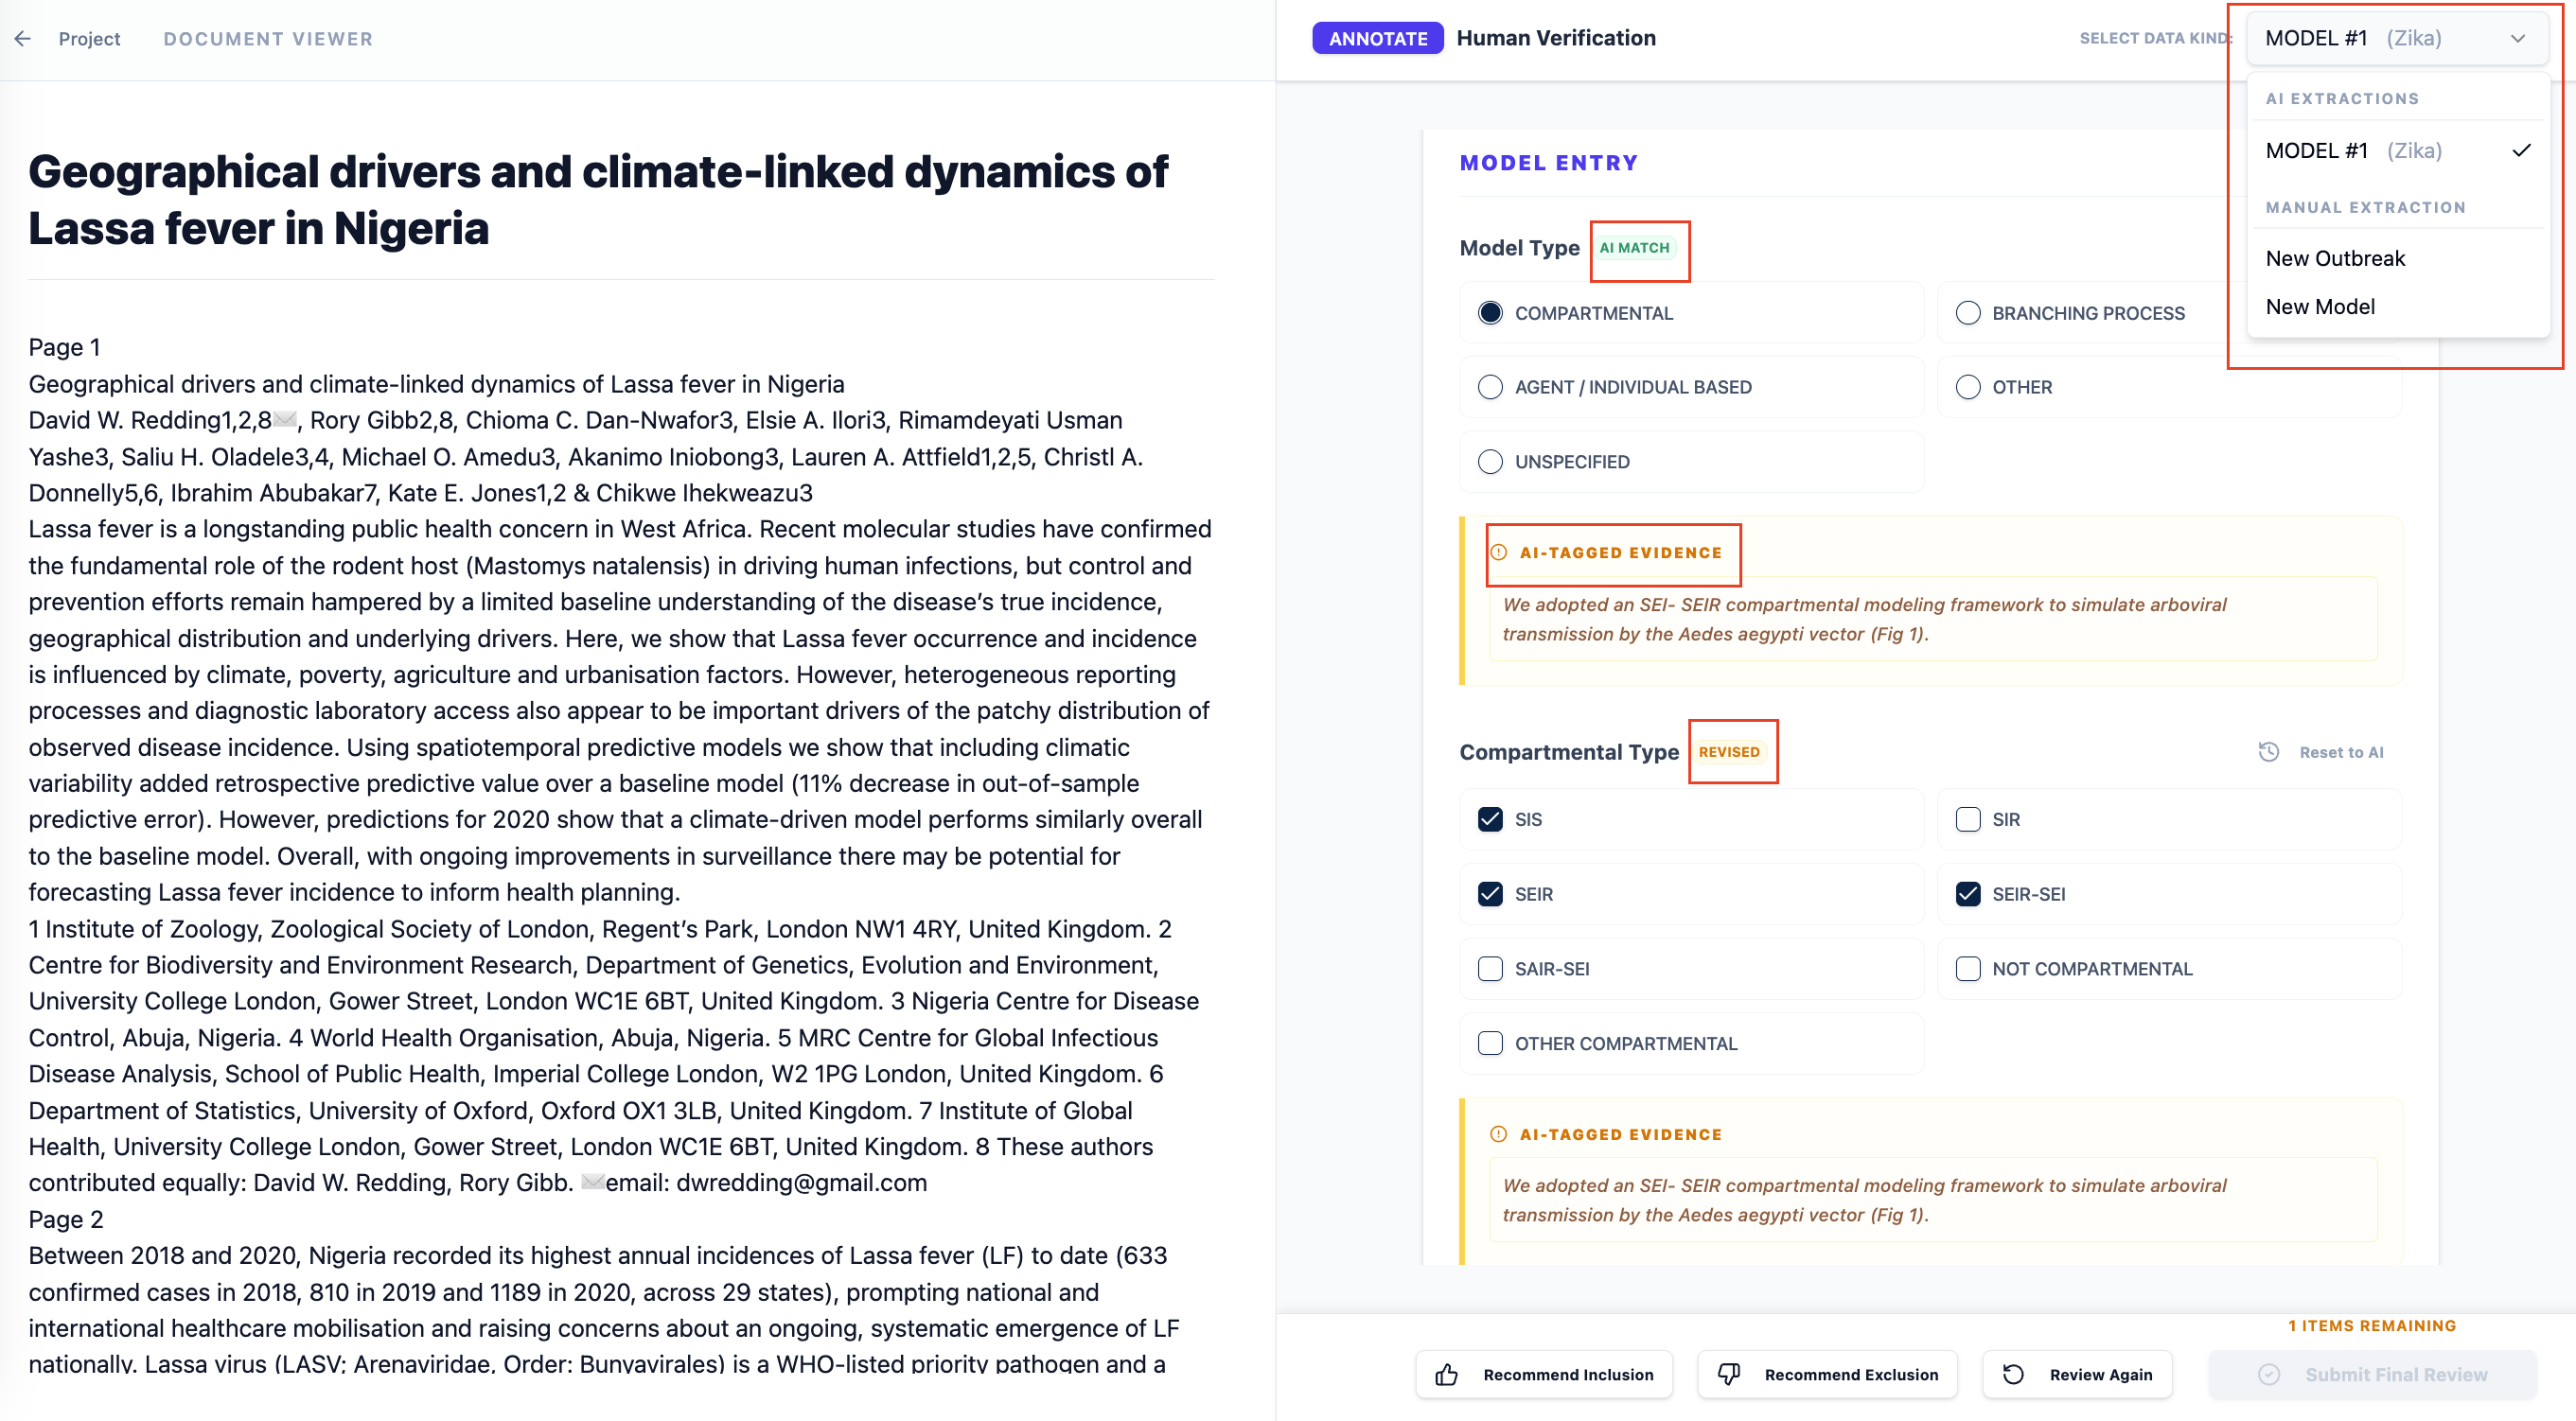
\includegraphics[width=0.95\textwidth]{figures/annotation/ann_tool_main.png}
    \caption{\textbf{The \name{} extraction and validation tool interface.} The dual-pane view presents the source document (\textbf{left}) alongside structured extraction fields (\textbf{right}). AI-predicted entries are pre-filled and accompanied by highlighted, AI-tagged evidence excerpts from the manuscript. Reviewers can accept, revise, or reject individual fields, with validation status indicators (e.g. ``AI Match'' or ``Revised'') reflecting whether human intervention was required.}
    \label{fig:ann_main}
\end{figure}

\subsection{System Architecture and Core Functionality}
The \name{} annotation tool provides an interactive environment for technical validation of automated information extractions. The system utilises data gathered by LLMs equipped with structured tool-calling to identify and parse epidemiological parameters, transmission models, and outbreak characteristics. To ensure transparency and auditability, the tool implements a provenance layer that maps every extracted value to specific textual excerpts (AI-tagged evidence) within the source article.

\subsection{User Interface Design}
The interface is optimised for high-throughput expert review via a dual-panel architecture:
\vspace{-10pt}
\begin{itemize}[leftmargin=*, itemsep=-3pt]
    \item \textit{Document Viewer (Left Panel):} Provides the original article text or rendered PDF, ensuring reviewers can verify the context of any extracted data point without context switching.
    \item \textit{Verification Interface (Right Panel):} Displays a form-based view of pre-filled fields generated by the \name{} pipeline. The extraction schema is dynamic, adapting based on the identified content type, such as compartmental model variables or spatio-temporal outbreak data.
\end{itemize}

\subsection{Human-in-the-Loop Validation}
The framework enforces a human-in-the-loop (HITL) protocol where automated extractions are audited by subject matter experts before being finalised for evidence synthesis. Within the interface, reviewers perform the following actions:
\vspace{-10pt}
\begin{itemize}[leftmargin=*, itemsep=-3pt]
    \item \textit{Verify:} Confirm the accuracy of the AI-extracted value and its linked evidence.
    \item \textit{Modify:} Correct extraction errors or refine data granularity; modified entries are flagged as ``Revised'' to facilitate system error analysis.
    \item \textit{Reject:} Entirely dismiss false positive extractions that do not meet inclusion criteria.
\end{itemize}

\subsection{Current Status and Field Testing}
The tool is currently in a beta development phase, with pilot testing conducted by epidemiologists focusing on WHO priority pathogens. While the current pilot utilises epidemiology-specific schemas, the architecture is designed to be domain-agnostic and can be adapted through schema reconfiguration and expert consultation.

Planned field testing is aligned with the Pathogen Epidemiology Review Group (PERG) workflow for remaining priority pathogens. This testing will utilise standardised extraction schemas for parameter, model, and outbreak data, and specifically target  systematic reviews for CCHF virus and Rift Valley fever virus.

\begin{figure}[t]
    \centering
    \begin{minipage}[b]{0.48\textwidth}
        \centering
        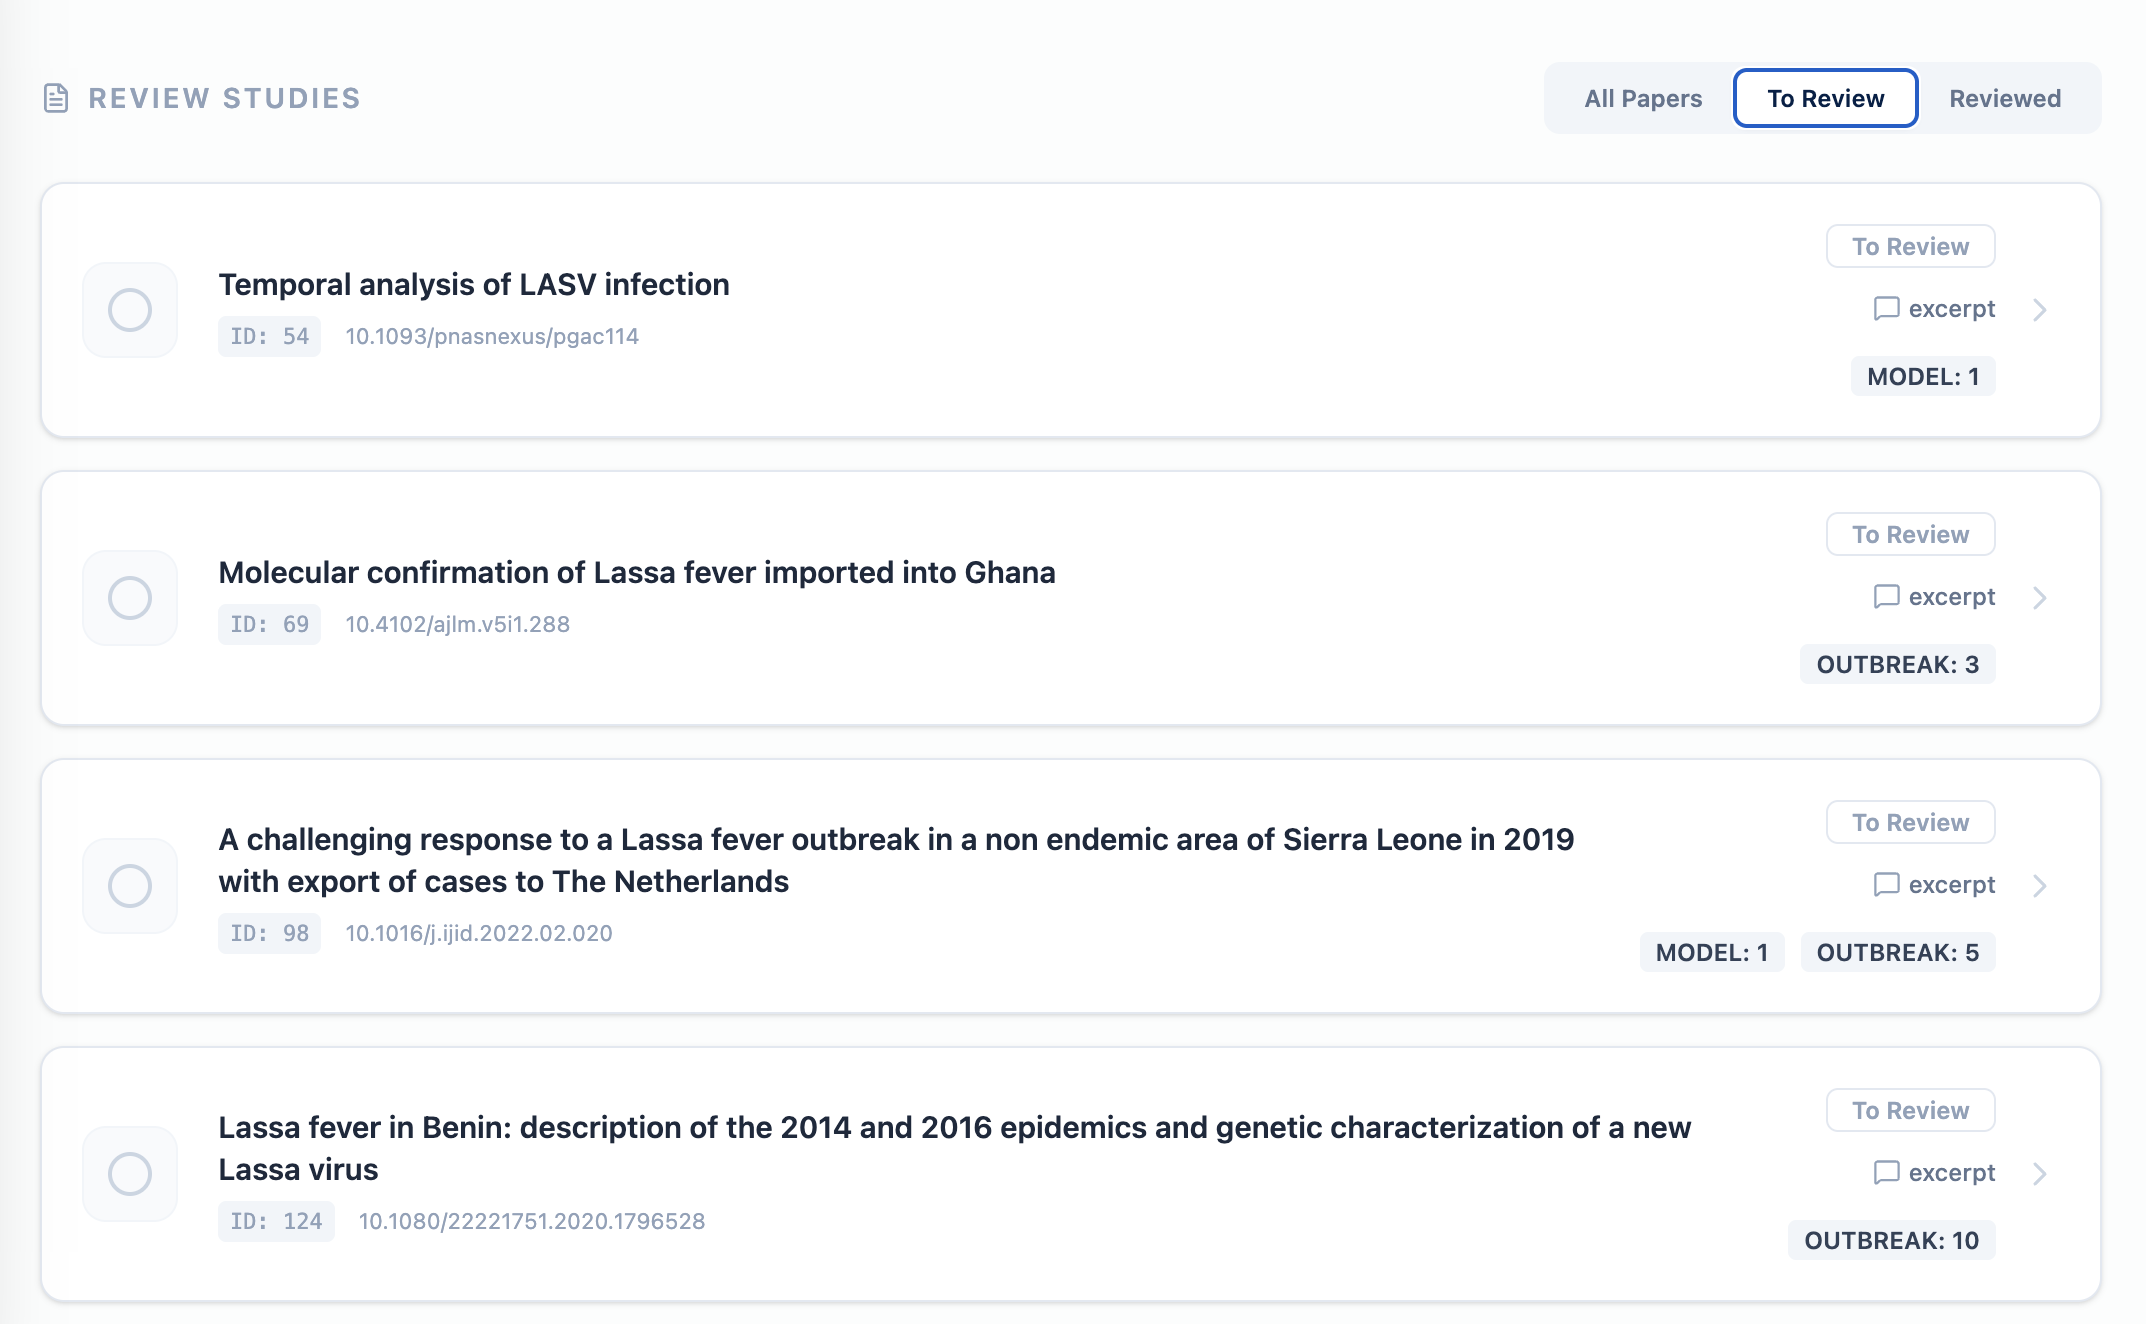
\includegraphics[height=5.7cm,keepaspectratio]{figures/annotation/ann_tool_multiple_papers_to_review.png}
        \caption*{(a) Tool Management Dashboard}
    \end{minipage}\hfill
    \begin{minipage}[b]{0.48\textwidth}
        \centering
        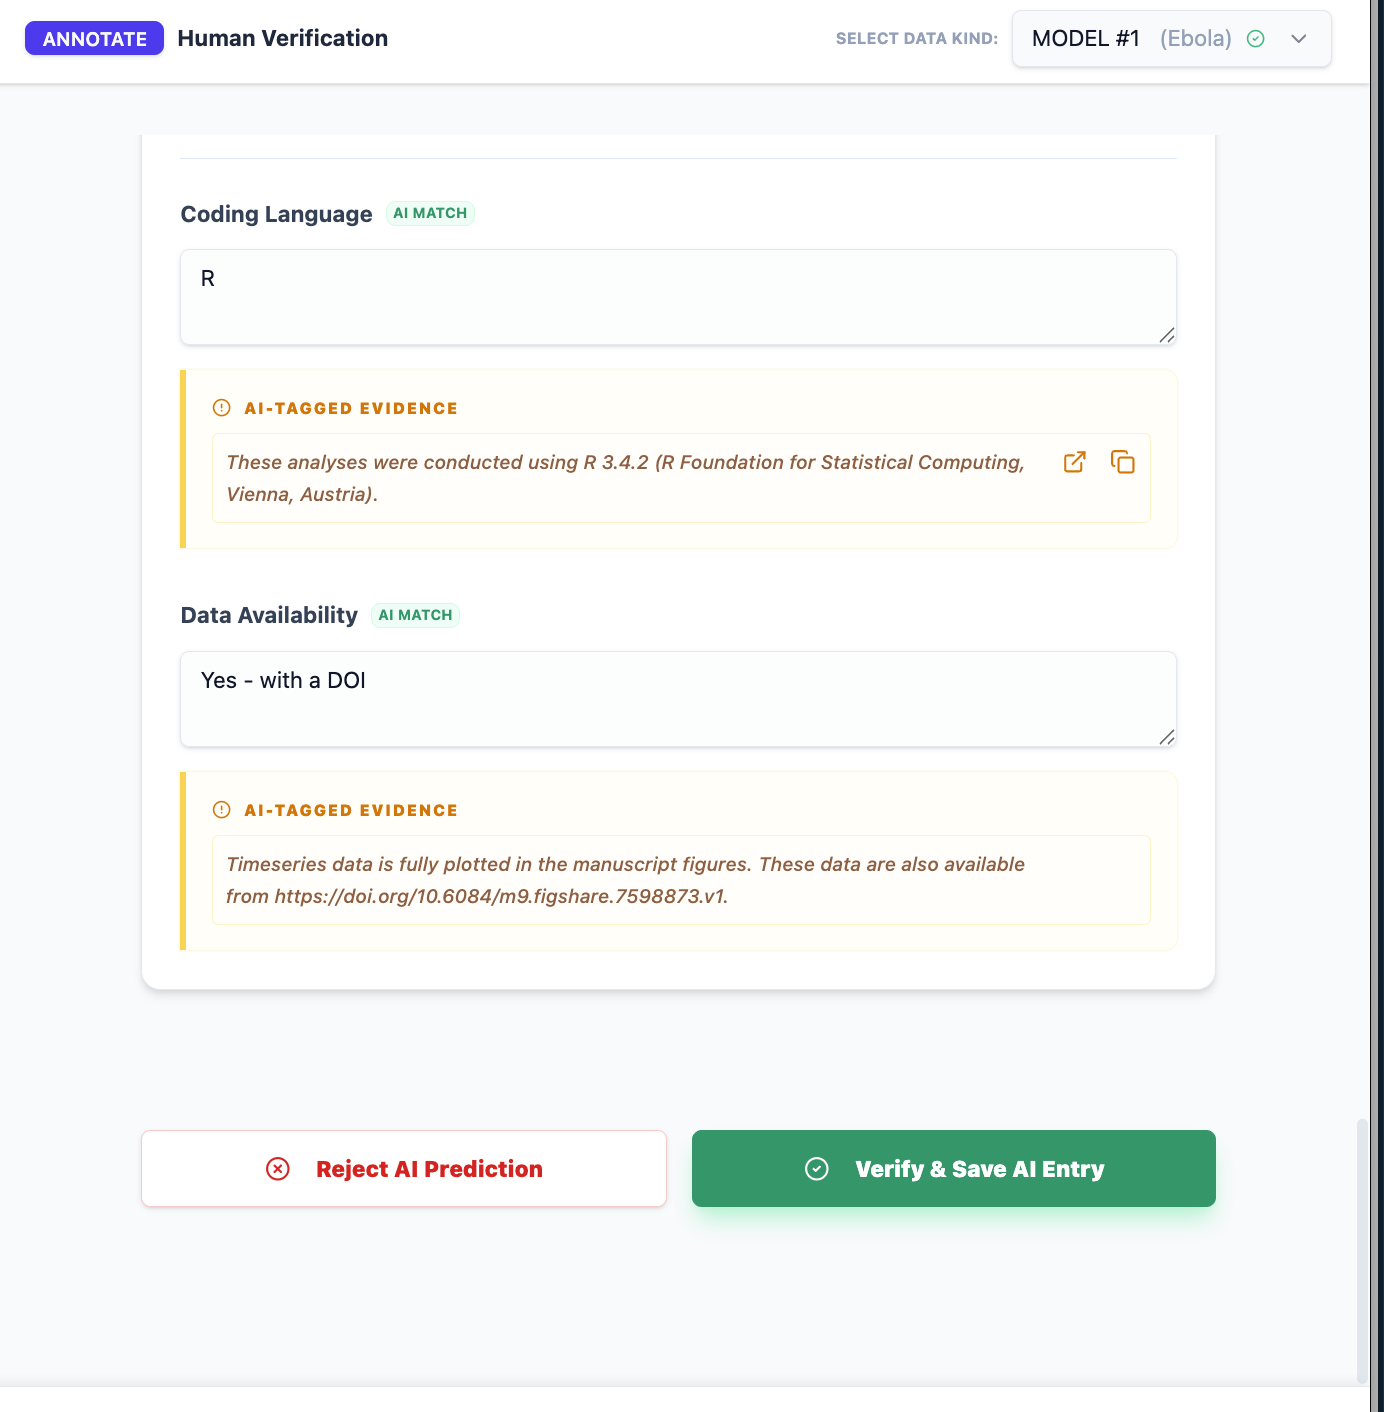
\includegraphics[height=5.2cm,keepaspectratio]{figures/annotation/ann_tool_verify_and_submit.png}
        \caption*{(b) Verification and Submission}
    \end{minipage}
    \caption{\textbf{Review management and submission tracking interfaces.} (a) The study review list displays papers awaiting expert validation, along with associated model and outbreak counts and direct links to extracted excerpts. (b) The verification view presents finalised AI-assisted extractions, enabling reviewers to explicitly reject predictions or verify and save corrected entries, which are then recorded for downstream quality control and system evaluation.}
    \label{fig:ann_logistics}
\end{figure}

\subsection{Transparency and Reproducibility}
By maintaining a persistent link between the structured database and the source text, \name{} ensures that synthesised reports can be fully disaggregated. This audit trail is critical for scientific reproducibility, allowing researchers to trace every reported parameter, model and outbreak back to its exact location in the primary literature.

\end{document}